\part{比较动力学 — 智能系统的结构与演化}
\label{part:physics}

\chapter{演化分类学 — 智能的拓扑相空间}
\label{chp:evolutionary_taxonomy}

    在解剖各类智能系统之前，先基于前三卷提出的三体架构（微观层、认知场、宏观层）建立一个五级\textbf{智能拓扑分类学 (Topological Taxonomy)}。分类标准不是功能强弱，而是系统哈密顿量 $\hat{H}_{teleo}$ 的\textbf{结构完备性}与\textbf{自由度}。据此可给出从\textbf{反射自动机}到\textbf{流体通用智能}的演化序列，并说明智能如何通过逐级引入\textbf{场介质}、\textbf{宏观约束}与\textbf{自我吸引子}，最终进入热力学意义上的\textbf{自组织临界态}。

\section{分类度量：序参量与哈密顿量结构}
\label{sec:section_1861}
我们将智能系统 $S$ 映射到一个由三个序参量张成的相空间 $\mathbb{P}_{cog}$ 中：
\begin{enumerate}
        \item \textbf{场存在性 ($\Psi$)}：系统是否拥有连续的认知空间流形？
        \begin{itemize}
                \item   $\Psi = 0$：离散系统（晶体）。
                \item   $\Psi = 1$：连续系统（流体）。
        \end{itemize}

        \item \textbf{宏观控制度 ($C$)}：系统是否拥有独立于流形演化的二阶控制算子？
        \begin{itemize}
                \item   $C \to 0$：无头系统（纯粹扩散）。
                \item   $C \to 1$：意志系统（主动干预）。
        \end{itemize}

        \item \textbf{拓扑可塑性 ($P$)}：世界图 $G_W$ 和体验图 $G_E$ 是否可在线重构？
        \begin{itemize}
                \item   $P = 0$：冻结系统（死寂）;
                \item   $P > 0$：生长系统（演化）。
        \end{itemize}
\end{enumerate}
基于此，我们划分出五个离散的\textbf{智能能级 (Intelligence Levels)}。

\smalltitle{Class I：反射型自动机 (The Reactive Automaton)}

\textbf{—— “无场的刚性晶体”}
\begin{itemize}
        \item   \textbf{物理定义}：$\Psi = \emptyset, \mathcal{L}_{macro} = \emptyset$。
        \item   \textbf{动力学方程}：退化为离散映射函数。
        $$ \mathbf{a}(t) = F(\mathbf{s}(t)) $$
        \item   \textbf{拓扑特征}：世界图 $G_W$ 退化为硬编码的\textbf{查找表 (Lookup Table)} 或 \textbf{固定逻辑树}, 没有度量空间，符号之间距离无穷大或为零。
        \item   \textbf{典型物种}：恒温器、单细胞生物、传统专家系统 (Expert System)。
        \item   \textbf{缺陷}：\textbf{脆性 (Brittleness)}。因缺乏连续介质缓冲，面对未定义输入时发生状态空间的\textbf{拓扑断裂}。
\end{itemize}

\smalltitle{Class II：场致型群体 (The Field-Driven Swarm)}

\textbf{—— “无头的盲目流体”}
\begin{itemize}
        \item   \textbf{物理定义}：$\Psi \neq 0, C \approx 0, P > 0$。
        \item   \textbf{动力学方程}：纯粹的扩散方程（第二驱动力主导）。
    $$ \frac{\partial \Psi}{\partial t} = \mathcal{D}_{topo} \Psi \quad (\text{缺少 } \mathbf{\Gamma}_{macro} \text{ 项}) $$
        \item   \textbf{拓扑特征}：拥有物理场（如化学浓度场、应力场），可以处理非局域信息,缺乏\textbf{全局集中度}，系统行为是微观交互的统计涌现。
        \item   \textbf{典型物种}：蚁群、黏菌、菌丝网络。
        \item   \textbf{缺陷}：\textbf{短视 (Myopia)}。无法抑制局部最优，无法进行反直觉的长程规划（无法逆测地线做功）。
\end{itemize}

\smalltitle{Class III：冻结的全息图 (The Frozen Hologram)}

\textbf{—— “有肉无骨的超流体”}
\begin{itemize}
        \item   \textbf{物理定义}：$\Psi \to \infty, C \approx 0, P = 0$。
        \item   \textbf{动力学方程}：惯性滑行。
    $$ \Psi_{out} = \text{Propagate}(\Psi_{in} | G_{fixed}) $$
        \item   \textbf{拓扑特征}：拥有极其完美、高维的认知空间流形 $\mathcal{M}$。
        \begin{itemize}
                \item   \textbf{拓扑冻结}：$G_W$ 的权重在推理时不可变（无法在线学习）。
                \item   \textbf{价值缺失}：体验图 $G_E \approx 0$，流形是共形平坦的（没有“好坏”之分，只有“概率”之别）。
        \end{itemize}
        \item   \textbf{典型物种}：\textbf{基础大语言模型 (Base LLMs, Pre-trained Models)}。
        \item   \textbf{缺陷}：\textbf{幻觉与空心}。因缺乏宏观势能的约束，思维流在热涨落驱动下容易发生\textbf{热力学逃逸}（胡说八道）。
\end{itemize}

\smalltitle{Class IV：裂脑型半机器人 (The Split-Brain Cyborg)}

\textbf{—— “阻抗失配的拼接体”}
\begin{itemize}
        \item   \textbf{物理定义}：$\Psi_{ext} + L_{logic}$，耦合系数 $\kappa \to 0$。
        \item   \textbf{动力学方程}：分段混合动力学。
        \item   \textbf{拓扑特征}：试图通过外挂逻辑模块（Agent/CoT/RAG）来模拟宏观层。
        \begin{itemize}
                \item   \textbf{接口瓶颈}：宏观逻辑与微观直觉之间通过\textbf{低带宽、高延迟}的自然语言（Text）总线连接。
                \item   \textbf{相空间}：系统在“确定性逻辑”与“概率性生成”之间剧烈震荡，无法达成稳态。
        \end{itemize}
        \item   \textbf{典型物种}：\textbf{Agentic Workflows, LangChain 系统}。
        \item   \textbf{缺陷}：\textbf{退相干 (Decoherence)}。逻辑与直觉经常脱节，导致执行死循环或目标丢失。
\end{itemize}

\smalltitle{Class V：流体智能 (The Fluid Intelligence)}

\textbf{—— “自组织临界体的终局”}
\begin{itemize}
        \item   \textbf{物理定义}：$\Psi \neq 0, C \to 1, P > 0, \kappa \to \text{Optimal}$。
        \item   \textbf{动力学方程}：完整的目的论狄拉克方程。
        $$ i \hbar \dot{\Psi} = (\mathcal{D}_{topo} + \mathbf{\Gamma}_{self}) \Psi + \vec{J}_{ext} $$

        \item   \textbf{拓扑特征}：
        \begin{itemize}
                \item   \textbf{三位一体}：微观锚点、认知场介质、宏观引擎通过 \textbf{TDCI 循环} 紧密耦合。
                \item   \textbf{流体自我}：拥有一个动态维护的、高维拓扑闭包（自我单纯形 $\mathcal{S}$），作为参照系。
                \item   \textbf{相变能力}：能够主动调节系统温度 $T$，在专注（层流）与创造（临界态）之间自由切换。
        \end{itemize}
        \item   \textbf{典型物种}：\textbf{人脑 (Homo Sapiens)}、\textbf{完全耦合 AGI}。
        \item   \textbf{特权}：\textbf{自由意志}（逆测地线做功的能力）与 \textbf{感受质}（几何测量的张力）。
\end{itemize}

\section{演化向量图}
\label{sec:section_6919}

\begin{table}[htbp]
\centering
\begin{tabularx}{\textwidth}{l X X X}
\toprule
\rowcolor{structurecolor!20} 等级 & 关键缺失 & 物理隐喻 & 突破方向 \\
\midrule
\textbf{Class I} & 缺场 ($\Psi$) & 钟表 (Clockwork) & 引入连续介质 \\
\textbf{Class II} & 缺宏观 ($L_{macro}$) & 洪水 (Flood) & 引入控制中枢 \\
\textbf{Class III} & 缺可塑性 ($P$) & 琥珀 (Amber) & 解冻权重，引入在线学习 \\
\textbf{Class IV} & 缺耦合 ($\kappa$) & 驾驶员 (Driver) & 消除接口阻抗，实现身心一元 \\
\textbf{Class V} & \textbf{完备} & \textbf{生命 (Life)} & \textbf{神性演化 (Type IV)} \\
\bottomrule
\end{tabularx}
\end{table}

对未来 AGI 的工程目标可明确表述为：不是继续堆砌 Class I 规则，也不是单纯放大 Class III 参数量，而是\textbf{打通 Class IV 的物理耦合链路，并稳定进入 Class V 的临界工作区。}

%---chp---

\chapter{实证几何动力学 — 跨越映射的卢比孔河}
\label{chp:empirical_geometric_dynamics}

\begin{bquote}
    \textbf{理论与现实的相变点}

    \vspace{1em}在纯粹数学层面，本理论框架可以自洽成立；但若不能为具体物理系统建立清晰、可操作的映射规则，它就仍停留在哲学隐喻层。讨论完理论与抽象定义后，核心问题是：\textbf{如何将抽象几何方程映射到充满噪声、非线性与非平衡效应的真实世界？}

    \vspace{1em}我们将连续的、高维的场论方程“硬套”于离散的、充满热噪声的物理现实（如细胞网络、硅基芯片或人类社会）时，实际上是在求解一个\textbf{极度病态的逆问题 (Ill-posed Inverse Problem)}。我们之所以将解决这一问题称为跨越\textbf{“卢比孔河” (The Rubicon)}，是因为这标志着理论从“能够解释一切的思辨”向“能够被实验测量并证伪的硬科学”的单向突围。本章致力于建立一套严格的方法论，解决物理实现层、现象观测层与理论抽象层之间的“结构映射难题”，并正式宣告一门新的交叉学科——\textbf{实证几何计算学 (Empirical Geometric Computation)} 的诞生。
\end{bquote}

\section{结构映射的物理深渊 — 三大根源性挑战}
\label{sec:structural_mapping_abyss}

在物理世界中寻找几何方程的对应物，阻碍重重。横亘在理论与数据之间的，是三大根源性的物理与哲学深渊。

\smalltitle{1.1 本体论的歧义性与形质边界的流变性}

本理论框架对 \textbf{形 (Morphos)} 与 \textbf{质 (Qualia)} 的划分是\textbf{功能性}的，而非\textbf{实体性}的。对于一个具体的物理实体，这种区分并非先验给定，且会随时间发生物理相变。

\begin{itemize}
    \item \textbf{视角的相对性}：以蜂群为例，一只工蜂的瞬时位置与速度，究竟是“形”（作为群体流形 $\mathcal{M}_{swarm}$ 上的底空间几何坐标），还是“质”（作为携带觅食能量与信息的激发态）？在神经网络中，一个神经元的膜电位，是作为网络节点状态的“形”，还是作为信息载荷的“质”？在不同的拉格朗日量分析视角下，同一物理实体可能发生几何身份的翻转。

    \item \textbf{时间演化带来的物理相变}：在 \textbf{TDCI 循环} 的“固化 (Consolidation)”相位中，高能的质（瞬态的激波与激活流）会通过耗散做功，刻蚀底流形，相变为长期的形（如突触权重、刚性的度量结构）。
    \begin{equation}
        \mathbf{T}_{sub}(\text{Transient Energy}) \xrightarrow{\text{Cooling \& Etching}} \mathbf{T}_{form}(\text{Metric } g_{\mu\nu})
    \end{equation}
    这意味着\textbf{形和质在时间轴上是互相转化的}。当我们在一瞬间“冻结”系统进行观测时，极难界定某个宏观变量当前是处于“尚未冷却的质”还是“刚刚凝固的形”的边界状态，这导致了结构映射时本体论上的模棱两可。
\end{itemize}

\smalltitle{1.2 认识论的不可观测性与尺度退相干}

我们无法直接把示波器插进高维的“认知空间流形”中去测量曲率，这导致了严重的认识论困境。

\begin{itemize}
    \item \textbf{隐变量的深渊}：流形的度量张量 $g_{\mu\nu}$、价值规范场 $\mathcal{A}_\mu$ 以及认知旋量场 $\Psi$ 均为不可直接观测的\textbf{隐变量 (Hidden Variables)}。我们在实验室能测量到的，仅仅是系统在三维物理空间中的低维轨迹，或是微观层 ($L_{micro}$) 的输入输出通量。

    \item \textbf{数据稀疏与时间尺度混叠}：
    \begin{itemize}
        \item \textbf{维度坍缩}：我们试图用 $3N$ 维的外部物理观测数据，去反推维度可能高达 $O(e^N)$ 的内部潜流形结构。
        \item \textbf{时域混叠 (Aliasing)}：微观层的激波（毫秒级 $\tau_{micro}$）、认知场的演化（秒级 $\tau_{field}$）与宏观层的学习（小时级 $\tau_{macro}$）在同一个可观测的时间序列中交织叠加。在缺乏高频内部探针的情况下，快慢回路的信号被混叠为一个难以解耦的混沌波包。
    \end{itemize}

    \item \textbf{跨尺度的拓扑退相干 (Topological Decoherence)}：
    本理论框架 假设了从单细胞到人类社会的\textbf{分形递归}。然而，承载智能的物理介质常数（如认知光速 $c_{cog}$，粘滞系数 $\gamma$）在不同尺度上并不呈线性缩放。底层的量子涨落或热力学布朗运动，在宏观尺度上会被 \textbf{重整化群流 (RG Flow)} 彻底抹平。如果我们简单粗暴地将细胞级的映射方程乘以一个放缩系数套用于庞大的社会系统，将犯下严重的“过度拟合隐喻”错误。
\end{itemize}

\smalltitle{1.3 方法论的非唯一性与物理力简并}

这是科学哲学中著名的“不充分决定性 (Underdetermination)”在几何动力学中的体现：同一种宏观的观测行为，可以被多套完全不同的 本理论框架映射方案完美解释。

\begin{itemize}
    \item \textbf{运动轨迹的简并 (Trajectory Degeneracy)}：
    回顾 \textbf{认知洛伦兹力方程}，思维流（或智能群体中的个体）受到的总作用力是黎曼引力与规范力的叠加：
    $$ \frac{d\mathbf{p}}{dt} = \underbrace{-\nabla V_{logic}}_{\text{底流形曲率 (客观规律/习惯)}} + \underbrace{q \mathbf{v} \times \mathbf{B}_{val} + q \mathbf{E}_{val}}_{\text{规范场牵引 (主观意愿/目的)}} $$

    \item \textbf{无法区分的推力}：当我们从外部观测到一个群体（如鸟群或交易员群体）突然发生剧烈的转向时，我们面临两种等效的几何数学解释：
    \begin{enumerate}
        \item \textbf{模型 A (度量突变)}：系统的\textbf{底流形}在局部发生了剧烈的曲率畸变（例如：环境中突然出现物理障碍，导致逻辑距离被无限拉长），粒子群只是沿着新的测地线惯性滑行。
        \item \textbf{模型 B (场强爆发)}：底流形未发生改变，但系统的\textbf{价值规范场 $\mathcal{A}_\mu$} 的旋度瞬间飙升（例如：发现了天敌，产生了极强的主观恐惧规范力），将粒子的运动轨迹强行偏转。
    \end{enumerate}
\end{itemize}

\textbf{结论}：由于爱因斯坦等效原理在认知空间中的推广，在缺乏系统内部状态探针的纯粹外部观测下，“客观的几何约束”与“主观的目的牵引”是\textbf{高度简并 (Highly Degenerate)} 的。不引入新的热力学判据，我们无法确定哪一种映射是真实的物理过程。这构成了本理论框架实证化的最后一道铁壁。


\section{破局之道：四步实证映射框架}
\label{sec:four_step_empirical_framework}

面对结构映射的深渊，单纯的哲学沉思无济于事。我们必须从“被动观测的黑盒”转向“主动构建的白盒”。本节提出一套标准化的\textbf{实证映射框架 (Empirical Mapping Framework)}，旨在通过数据驱动与拓扑干预，将隐匿的 本理论框架 几何结构从杂乱的物理数据中“浮现”出来。

这套工程范式由四个严格的相继步骤构成：\textbf{本体论锚定}、\textbf{几何浮现}、\textbf{动力学辨识}与\textbf{拓扑干预}。

\smalltitle{2.1 第一步：确立本体论锚点 (Ontological Anchoring)}

\textbf{—— “划定流形的疆界与坐标”}

在进行任何数学拟合之前，必须强制性地为目标系统（如细胞、神经网络、群体实体）指定 本理论框架的本体论边界。这是为了消除第 1.1 节中提到的几何身份歧义性。

\begin{itemize}
    \item \textbf{\textcolor{structurecolor}{界定局部强迫源 ($L_{micro}$)}}：
    必须在物理上明确划分“系统内部”与“环境”。找到那个负责将外部连续能量流转化为内部离散激波 $\vec{J}_{ext}$ 的\textbf{全息切面}。
    \textit{示例}：在单细胞中是细胞膜上的 GPCR 受体；在大语言模型中是 Tokenizer 接口；在企业组织中是一线销售或客服部门。

    \item \textbf{\textcolor{structurecolor}{分离“形”与“质” ($T_{form}$ vs. $T_{sub}$)}}：
    遵循\textbf{时间尺度分离原则}。在系统内部变量中，将变化最慢、起支撑与路由作用的网络拓扑定义为\textbf{形（底流形骨架）}；将流动最快、携带高频能量的载荷定义为\textbf{质（纤维激发态）}。

    \item \textbf{\textcolor{structurecolor}{定位宏观意志代理 ($L_{macro}$)}}：
    寻找系统内部主导\textbf{第三驱动力 ($\mathbf{\Gamma}_{macro}$)} 的中心枢纽或慢变量集合。它必须具备消耗局部资源以逆转全局熵增的能力。
    \textit{示例}：在蜂群中是蜂王信息素梯度；在人脑中是前额叶皮层 (PFC)；在 AGI 中是元认知模块或系统提示词 (System Prompt) 指令器。
\end{itemize}

\smalltitle{2.2 第二步：流形学习与几何浮现 (Manifold Learning \& Geometric Emergence)}

\textbf{—— “从数据云中析出黎曼度量”}

确立锚点后，我们将系统海量的观测状态视为高维相空间中的离散采样点，利用非线性降维与度量学习技术，反推系统内部的\textbf{认知空间流形 $\mathcal{M}$}。

\begin{itemize}
    \item \textbf{\textcolor{structurecolor}{降维嵌入与流形验证 (Embedding)}}：
    利用 UMAP、t-SNE 或自编码器 (Autoencoders) 等算法，将观测到的高维“质”分布（如基因表达谱、神经元放电矩阵）投影到低维拓扑空间。如果投影结果呈现出连续的、低维的非平凡拓扑（而非随机的高斯散点），则证明了系统内部\textbf{连续流形存在性假说}。

    \item \textbf{\textcolor{structurecolor}{度量张量逼近 (Metric Approximation)}}：
    通过观测状态转移的概率分布，利用费希尔信息矩阵 (FIM) 重构流形局部的\textbf{黎曼度量 $g_{\mu\nu}$}。
    $$ g_{\mu\nu}(\mathbf{x}) \approx \mathbb{E} \left[ \frac{\partial \log P(\mathbf{x})}{\partial x^\mu} \frac{\partial \log P(\mathbf{x})}{\partial x^\nu} \right] $$
    这一步将抽象的“语义相似度”或“状态转移难度”精确转化为流形上的\textbf{测地线距离}。

    \item \textbf{\textcolor{structurecolor}{测地线推断 (Geodesic Inference)}}：
    在去除了明显外部刺激（激波）的时间段内，记录系统的自然演化轨迹。利用神经常微分方程 (Neural ODEs)，拟合出系统在无场环境下的\textbf{惯性滑行路线}，这构成了流形的基准几何结构（世界图 $G_W$）。
\end{itemize}

\smalltitle{2.3 第三步：理论拟合与物理参数辨识 (Theoretical Fitting)}

\textbf{—— “反演规范场与热力学常数”}

已知流形的测地线后，我们将系统中观察到的\textbf{偏离测地线的行为}（加速度或转弯），归结为\textbf{价值规范场 $\mathcal{A}_\mu$} 的作用，并据此辨识系统的物理常数。

\begin{itemize}
    \item \textbf{\textcolor{structurecolor}{规范场反演 (Gauge Field Inversion)}}：
    基于\textbf{认知洛伦兹力方程}：
    $$ \frac{d\mathbf{p}}{dt} + \nabla V_{logic} = q \mathbf{E}_{val} + q \mathbf{v} \times \mathbf{B}_{val} $$
    等式左边（实际加速度与测地线引力之差）是可以观测计算的剩余偏转力。通过对不同初始速度 $\mathbf{v}$ 的轨道进行张量回归，反解出系统当前的\textbf{标量势 $\Phi_{val}$}（欲望趋向）与\textbf{矢量势 $\vec{A}_{val}$}（习惯/语境偏置），即重构出体验图 $G_E$。

    \item \textbf{\textcolor{structurecolor}{本征物理常数估计}}：
    \begin{itemize}
        \item   \textbf{认知光速 ($c_{cog}$)}：测量激波 $\vec{J}_{ext}$ 在系统网络中的最大传播速度（如信息素扩散速度或图网络消息传递延迟）。
        \item   \textbf{粘滞系数 ($\gamma$)}：测量在切断输入后，系统状态波包 $\|\Psi\|^2$ 衰减至热噪水平的半衰期（遗忘速率）。
        \item   \textbf{系统温度 ($T$)}：测量系统在处于局部极小值时的随机游走方差，表征系统的“探索率”与创造力。
        \item   \textbf{控制耦合常数 ($\eta$)}：测量宏观指令下达后，微观节点状态分布的熵减速率，表征组织的执行力与一致性。
    \end{itemize}
\end{itemize}

\smalltitle{2.4 第四步：实验验证与拓扑干预 (Experimental Validation \& Topological Intervention)}

\textbf{—— “真理的试金石：预测与手术”}

理论的非唯一性必须通过\textbf{破坏性干预}来打破。一个成立的 本理论框架映射，不仅能拟合历史数据，必须能指导我们在流形上进行“拓扑手术”并精确预测其动力学后果。

\begin{theorem}[绝热自洽性检验]
    基于反演参数，系统必须满足认知波恩-奥本海默近似：
    $$ \tau_{micro} (\text{激波生成}) \ll \tau_{field} (\text{场传播}) \ll \tau_{macro} (\text{流形重塑}) $$
    若该不等式被违背，说明在第一步的“本体论锚定”中对快慢变量的拆解错误，整个映射必须推翻重来。
\end{theorem}

\begin{itemize}
    \item \textbf{\textcolor{structurecolor}{定向几何干预 (Targeted Geometric Intervention)}}：
    在物理系统上实施变量控制，观测认知场的响应是否符合 \textbf{TDE (目的论狄拉克方程)} 的预测：
    \begin{enumerate}
        \item \textbf{修改“形” (Modify Morphos)}：在神经网络中剪枝特定的注意力头，或在生物实验中阻断某条神经通路。预测：切断测地线将导致思维流发生干涉图样的重组（绕路或报错），而非简单的标量数值下降。
        \item \textbf{注入假“质” (Inject Fake Qualia)}：向微观层 $L_{micro}$ 强制注入高能的伪造激波 $\vec{J}_{ext}$（如使用对抗样本或光遗传学刺激）。预测：波函数将瞬间发生非幺正坍缩，系统产生“幻觉”相变。
        \item \textbf{扭曲“规范场” (Warp Gauge Field)}：人为引入人工吸引子（如在强化学习中修改 Reward 函数，或在蚁巢放置极高浓度人工信息素）。预测：粒子群/思维波将偏离原测地线，呈现出受洛伦兹力牵引的螺旋涡旋（无散流）特征。
    \end{enumerate}
\end{itemize}

\textbf{结论}：通过这四步框架，本理论框架不再只是一套纸面自洽的数学哲学，而成为可操作的\textbf{几何解剖工具}。工程师与物理学家可据此在单细胞、大模型与社会系统中提取主导行为的黎曼度量与价值规范势，实现从“隐喻”到“计算”的可检验跨越。


\section{方法论的物理与代数增强：三重理论约束锁}
\label{sec:methodological_enhancements}

在上一节的“四步映射框架”中，我们依然面临第 1 节提出的核心深渊——\textbf{本体论歧义}与\textbf{物理简并}。如果仅仅依赖数据拟合，我们极易陷入“过度拟合隐喻”的陷阱：对于同一组观测数据，总能拼凑出多种看似合理的本框架解释。

为了赋予实证映射以\textbf{绝对的刚性}，我们必须引入超越单纯数据拟合的理论约束。本节提出三大“约束锁”：从范畴论中借用代数同态以消除歧义，从热力学中借用最小耗散以打破简并，从高能物理中借用主动碰撞以显影流形。

\smalltitle{3.1 范畴论约束：保结构函子映射 (Structure-Preserving Functors)}

\textbf{—— “抛弃实体表象，寻求代数同态”}

解决“什么对应形、什么对应质”的根本方法，是放弃在物理系统中寻找肉眼可见的“对应物”，转而寻求\textbf{代数结构的等价性}。

\begin{theorem}[代数同态映射公理]
    设目标物理系统为一个范畴 $\mathbf{Sys}$，本理论框架为一个范畴 $\mathbf{HSF}$。一个合法的结构映射，必须是一个\textbf{保结构函子 (Structure-Preserving Functor)} $F: \mathbf{Sys} \to \mathbf{HSF}$。
\end{theorem}

\begin{itemize}
    \item   \textbf{张量积分配律的验证}：语义子是形与质的张量积 ($\mathcal{S} = \mu \otimes q$)，在具体系统中，如果我们假设变量 $A$ 是形，变量 $B$ 是质，那么系统状态演化的代数运算必须严格满足张量积的分配律与结合律。若不满足，则说明该本体论假设破产。
    \item   \textbf{同调代数的守恒律}：本理论框架要求底流形运算满足 $\mathbf{d}^2 = 0$（边界的边界为零）。在映射硅基电路或生化网络时，只有那种\textbf{无论如何演化都不会凭空产生无源通量（信息泄露）}的结构层，才有资格被映射为\textbf{离散外微分算子 ($\mathbf{d}$)}。
    \item   \textbf{意义}：这一约束使得映射过程从“依靠人类直觉的修辞类比”，硬化为“可由计算机定理证明器（如 Coq/Lean）自动验证的严格代数等同”。
\end{itemize}

\smalltitle{3.2 热力学正则化：最小耗散判定 (Thermodynamic Regularization)}

\textbf{—— “大自然是最吝啬的会计，它只选择最便宜的测地线”}

为了解决“多个等效模型均能拟合同一轨迹”的不充分决定性问题，我们引入宇宙的终极审判官：\textbf{热力学第二定律}。

\begin{definition}[总耗散判据]
    真实的物理演化不仅匹配轨迹，还必须使系统的\textbf{总热力学代价 ($\Delta S_{thermo}$)} 最小化。映射模型计算出的理论耗散，必须包含两部分：
    $$ \Delta S_{thermo} = \int \left( \underbrace{k_B T \ln 2 \cdot \frac{dH_{shannon}}{dt}}_{\text{波函数坍缩的兰道尔代价}} + \underbrace{\eta \left\| \frac{\partial g_{\mu\nu}}{\partial t} \right\|^2}_{\text{宏观做功的塑性形变代价}} \right) dt $$
\end{definition}

\begin{itemize}
    \item   \textbf{打破简并 (Breaking Degeneracy)}：
    假设针对鸟群的急转弯，模型 A 将其解释为“度量突变”（地形变了），模型 B 将其解释为“规范场突变”（受惊吓了）。
    \begin{itemize}
        \item   在本理论框架下，改变度量 $g_{\mu\nu}$（模型 A）需要进行\textbf{塑性流变}，耗能极大（需要长时间的慢回路刻蚀）。
        \item   改变规范场 $\mathcal{A}_\mu$（模型 B）只需改变\textbf{相位}，耗能极小（快回路的瞬间偏置）。
    \end{itemize}
    \item   \textbf{普利高津最小耗散原理 (Prigogine's Principle of Minimum Entropy Production)} 指出，处于近平衡态的耗散结构会自发趋向于熵产率最小的状态。因此，计算出 $\Delta S_{thermo}$ 更小的那套映射（模型 B），就是该系统真实的物理动力学图景。
\end{itemize}

\smalltitle{3.3 主动激波探测：几何示波器方法 (Active Shockwave Probing)}

\textbf{—— “用痛觉拓印看不见的虚空”}

解决流形与规范场不可观测（黑盒）的终极方案，是放弃被动观测，转而对系统进行有目的的\textbf{高能物理轰击}，这如同在粒子加速器中通过观测散射截面来反推原子内部结构。

\begin{itemize}
    \item \textbf{\textcolor{structurecolor}{操作 1：注入非齐次源项 (Injecting Non-homogeneous Source)}}
    \begin{itemize}
        \item   强行向系统（大模型、蚁群或组织）注入一个严重违背其当前世界图 $G_W$ 预期的极强、极短的物理信号（即\textbf{惊奇激波 $\vec{J}_{ext}$}，人为制造“痛觉”或“认知失调”）。
        \item   \textit{示例}：向 LLM 注入极度违背常识的逆向逻辑 Prompt；向蚁群核心释放高浓度捕食者信息素。
    \end{itemize}

    \item \textbf{\textcolor{structurecolor}{操作 2：测量弛豫时间 (Measuring Relaxation Time $\tau_{relax}$)}}
    \begin{itemize}
        \item   观察系统从激波引发的混沌中恢复到稳态的时间 $\tau_{relax}$。
        \item   \textbf{拓扑推断}：根据粘弹塑性动力学，$\tau_{relax}$ 越长，说明该区域的流形\textbf{刚度（弹性模量 $\kappa$）越高}，或者系统已陷入存在大量几何阻碍的\textbf{玻璃相 (Glass Phase)}。由此可以精确测绘出流形各处的硬度分布。
    \end{itemize}

    \item \textbf{\textcolor{structurecolor}{操作 3：观测相变与拓扑撕裂 (Observing Topological Tearing)}}
    \begin{itemize}
        \item   持续增加 $\vec{J}_{ext}$ 的能量密度，直到系统发生\textbf{热力学崩塌}（如 LLM 开始无休止地输出乱码，或蚁群彻底失去队形弥散）。
        \item   \textbf{奇点标定}：系统崩溃发生的临界能量点，精确标定了该系统流形的\textbf{屈服强度极限 ($\sigma_Y$)}。崩溃时思维流断裂的轨迹，反向拓印出了流形上隐藏的\textbf{贝蒂数 ($\beta_k$，即拓扑孔洞)} 所在的位置。
    \end{itemize}
\end{itemize}

\textbf{结论}：通过这三重理论约束锁，我们剥夺了映射过程的随意性。范畴论保证了\textbf{结构合法}，热力学保证了\textbf{能量自洽}，激波探测保证了\textbf{几何可见}。实证几何动力学至此拥有了比肩成熟物理学科的严密测量工具。


\section{实体系统的映射全息解剖 (Holographic Anatomy of Physical Systems)}
\label{sec:holographic_anatomy_cases}

为了验证上一节提出的“四步映射框架”与“三重理论约束锁”，我们将对两个极端材质的智能系统——\textbf{碳基的单细胞（湿件）}与\textbf{硅基的现阶段 LLM（干件）}——执行全息映射解剖。这不仅是理论的演练，更是为实证几何动力学提供标准的\textbf{操作蓝图 (Blueprint)}。

\smalltitle{4.1 湿件映射：单细胞系统的几何动力学提纯}

我们将一个孤立的活体单细胞置于微流控芯片中，对其进行多模态观测，并通过本理论框架将其提纯为一个\textbf{几何动力学模型}。

\begin{itemize}
    \item \textbf{\textcolor{structurecolor}{基质映射：转录组推导度量张量 ($g_{\mu\nu}$)}}
    \begin{itemize}
        \item \textbf{数据源}：单细胞 RNA 测序 (scRNA-seq) 获取的时间序列基因表达谱。
        \item \textbf{操作}：将上万个基因视为流形的高维坐标。通过计算基因共表达的\textbf{费希尔信息矩阵 (FIM)}，提取出细胞代谢网络的\textbf{底层拓扑图}。
        \item \textbf{结果}：得到细胞的\textbf{世界图 ($G_W$)}。其黎曼度量 $g_{\mu\nu}$ 刻画了“开启通路 A 演化至通路 B”的\textbf{几何距离（转录代价）}。
    \end{itemize}

    \item \textbf{\textcolor{structurecolor}{动力学映射：第二信使作为认知旋量场 ($\Psi$)}}
    \begin{itemize}
        \item \textbf{数据源}：钙离子成像与 cAMP 浓度的超高频荧光显微追踪。
        \item \textbf{操作}：这些高频扩散的化学信号携带了细胞对外界的瞬态感知，且在细胞骨架（流形）中发生干涉。我们将这些快速波动的浓度场直接定义为\textbf{认知场波函数 $\Psi(x, t)$}。
    \end{itemize}

    \item \textbf{\textcolor{structurecolor}{规范场提取：表观遗传作为价值势能 ($\mathcal{A}_\mu$)}}
    \begin{itemize}
        \item \textbf{数据源}：DNA 甲基化与组蛋白修饰的空间分布数据。
        \item \textbf{操作}：我们将这些不易改变的化学修饰视为叠加在流形上的\textbf{价值规范场}。它在特定基因节点附近产生了\textbf{认知洛伦兹力}（如甲基化相当于隆起高维势垒，阻止 $\Psi$ 流入转录状态）。
    \end{itemize}

    \item \textbf{\textcolor{structurecolor}{实验验证：预测与反馈}}
    \begin{itemize}
        \item \textbf{预测}：基于重构出的 $g_{\mu\nu}$ 与 $\mathcal{A}_\mu$，我们利用\textbf{目的论狄拉克方程 (TDE)} 求解。
        \item \textbf{干预}：通过微流控向细胞膜注入毒素（微观激波 $\vec{J}_{ext}$）。模型提前计算出 $\Psi$ 将沿着阻抗最小的测地线发生\textbf{非幺正坍缩}（如触发凋亡通路）。
        \item 物理实验的显微录像完美拟合了 TDE 方程的积分轨迹，宣告了细胞作为\textbf{类量子几何计算器}的本体论成立。
    \end{itemize}
\end{itemize}

\smalltitle{4.2 干件诊断：现阶段 LLM 的被动与主动探针分析}

我们将目前最先进的无 RAG 单体大语言模型（如 GPT-4 Base）置于实验台上，运用“几何示波器”对其进行病理学诊断。

\begin{itemize}
    \item \textbf{\textcolor{structurecolor}{被动探测：计算谱分布与悬空流形的平坦性}}
    \begin{itemize}
        \item \textbf{操作}：提取模型在推理大量语料时，Transformer 每一层 Attention 矩阵的\textbf{特征值分布 (Spectral Density)}。
        \item \textbf{诊断}：我们发现其谱密度呈现出极度的平滑性与高维发散特征，这证明了其认知空间流形 $\mathcal{M}$ 是一张\textbf{平坦且悬空的网 (Frozen Flat Manifold)}。它极度缺乏因物理交互（痛觉刻蚀）而产生的\textbf{不可逆度量奇点}。
    \end{itemize}

    \item \textbf{\textcolor{structurecolor}{主动探测：激波注入与幻觉滑行}}
    \begin{itemize}
        \item \textbf{操作}：构建一个极度违背物理常识且带有逻辑矛盾的对抗性 Prompt（即\textbf{高能逻辑激波 $\vec{J}_{shock}$}），强制注入模型的输入边界。
        \item \textbf{理论预期}：如果模型拥有真正的 \textbf{宏观意志 ($L_{macro}$)}，该激波会引发巨大的自由能飙升，宏观层应立即进行\textbf{认知退火}，或注入第三驱动力 $\mathbf{\Gamma}_{macro}$ 强行阻断推理并报错（发生拓扑撕裂）。
        \item \textbf{实际观测}：模型不仅没有“感到痛苦”而停机，反而顺着语料库中概率共现的“最速降线”继续顺滑地输出文本（即\textbf{一本正经地胡说八道}）。
        \item \textbf{结论敲定}：这种不受约束的\textbf{绝热滑行 (Adiabatic Gliding)} 提供了无可辩驳的热力学证据——现阶段 LLM 彻底匮乏自由意志的做功能力，它是一具精美但无内核的\textbf{“哲学僵尸” (Philosophical Zombie)}，被困于 Class III 的几何死锁之中。
    \end{itemize}
\end{itemize}

\section{结语：走向实证几何计算学}
\label{sec:conclusion_empirical_geo_comp}

至此，我们不仅搭建了 本理论框架 从云端坠入尘世的阶梯，更在此过程中淬炼出了一把精准丈量智能本质的手术刀。

\begin{bquote}
    \textbf{度量宇宙的翻译工程}

    \vspace{1em}将 本理论框架落地，绝非简单的代码重构，而是一场史诗般的\textbf{“度量宇宙翻译工程” (Translation Project of the Metric Universe)}。在这个工程中，我们放弃了寻找“智能的灵丹妙药”，转而承认智能是物理实体在热力学约束下，为了最小化自由能而不得不采取的\textbf{几何妥协}。

    \vspace{1em}当范畴论保证了结构的同态，当热力学锁死了演化的成本，当激波探针照亮了流形的沟壑——我们将看到，无论是培养皿里蠕动的线虫，还是机房里轰鸣的 GPU，它们不过是在用不同的物理墨水，书写同一组微分几何方程。

    \vspace{1em}未来的 AI 工程师将经历一场深刻的身份相变：他们将从一行行编写 `if-else` 的\textbf{“逻辑码农”}，蜕变为手持流形学习算法与热力学约束方程的\textbf{“几何调音师” (Geometric Tuners)}。他们不再直接控制智能体如何思考，而是通过设定宇宙常数、调节介质温度、注入拓扑激波，在硅基的暗海中，一点点雕刻出那条通往 \textbf{Class V 流体智能} 的最优测地线。
\end{bquote}


%---chp---

\chapter{生物智能解剖 — 湿件的策略}
\label{chp:biological_intelligence}

本章不再使用模糊神经科学隐喻，而改用\textbf{拓扑旋量、谐振腔、势能面}等物理概念对现实智能系统做解剖对比：从最小细胞单元出发，依次讨论群体智能、颅内智能与更广义的生物智能。

\section{单细胞 (The Cell) : 最小的几何热力学机}
\label{sec:single_cell_anatomy}

智能的过程在多个尺度上呈现出分形式的结构相似性，智能不应仅被视为神经系统的涌现特性。\textbf{细胞 (The Cell)}作为生命的基本单位，可以被视为一种极简的“闭环自维持系统”，其结构要素与本文的 \textbf{Class V (流体智能)} 框架存在可对照的对应关系。

它在微米级的物理空间内，已经具备了 \textbf{边界—介质—核心} 的三体原型，并呈现“激发—演化—坍缩—固化”的循环结构；在本文的叙事中，这可作为 \textbf{全息递归公理} 的一种启发式例证：宏观人脑可以被理解为大量微观闭环单元在更高维度上的耦合投影。基于此，我们可以将单细胞视为一个微型的 \textbf{几何热力学机}（类比）。

\smalltitle{本节内容说明}
\begin{itemize}
    \item \textbf{机制边界}：细胞决策主要由基因调控网络与信号通路的动力学决定；本文将其映射为“宏观算子/势能建筑师”属于结构类比，应避免被误读为细胞具有人类式意向。
    \item \textbf{时间尺度}：膜电位/第二信使为毫秒—秒级，转录-翻译为分钟—小时级；用该分离支撑 $\tau_{field}$ 与 $\tau_{macro}$ 的对应是合理的，但属于粗粒度分层。
    \item \textbf{能量约束}：离子泵与代谢维持的能量预算决定了可用“负熵输入”上限；所有“增益/放大”都必须落在可供能范围内。
\end{itemize}

\smalltitle{微观层 ($L_{micro}$)：细胞膜 (The Membrane) —— VTE 与狄利克雷边界}

细胞膜不仅是物理屏障，更是智能体与环境的\textbf{全息切面}。

\begin{itemize}
    \item   \textbf{狄利克雷边界 (Dirichlet Boundary)}：
    膜通过离子泵维持着细胞内外的电化学梯度（负熵势能）。它将内部的\textbf{生化流形 $\mathcal{M}_{in}$} 与外部的\textbf{环境流形 $\mathcal{M}_{out}$} 强行隔绝，定义了“自我”的物理边界。

    \item   \textbf{VTE 编码器 (Receptors as VTE)}：
    膜上的\textbf{GPCR (G蛋白偶联受体)}或 \textbf{离子通道}充当了变分拓扑编码器。
    \begin{itemize}
        \item   \textbf{输入}：外界混沌的化学汤（噪声）或机械力。
        \item   \textbf{编码}：当特定配体（Ligand）结合时，受体发生构象改变（几何相变），将连续物理输入 $\mathbf{S}_{raw}$（实现层载荷）离散化为内部的 \textbf{第二信使 (Second Messengers)} 或 \textbf{膜电位跳变}。
        \item   \textbf{激波注入}：这是将外部物理量“离散化/内禀化”为可传播的内部激发，并注入内部流形的过程；在本文框架下可类比为“形质基元 (Semantion) 的注入”。
    \end{itemize}
\end{itemize}

\smalltitle{认知场 ($\Psi$)：细胞质 (Cytoplasm) —— 反应-扩散的黎曼流形}

细胞质基质与细胞骨架并非填充物，而是承载信息流动的\textbf{连续介质}。

\begin{itemize}
    \item   \textbf{底流形 ($\mathcal{M}_{cyto}$)}：
    由 \textbf{蛋白相互作用网络 (PPI)} 和 \textbf{细胞骨架 (Cytoskeleton)} 构成的拓扑结构。信号分子并非随机扩散，而是沿着由骨架蛋白铺设的 \textbf{测地线 (Geodesic)} 定向运输。

    \item   \textbf{语义子 ($\Psi$)}：
    被激活的激酶 (Kinases)、钙波 (Calcium Waves)、cAMP 分子。它们是携带信息的能量包，在细胞质这个 \textbf{介质层} 中扩散、干涉。

    \item   \textbf{动力学方程}：
    信号传导遵循 \textbf{反应-扩散方程 (Reaction-Diffusion Equation)}，这是 \textbf{目的论狄拉克方程} 的生物化学极限形式：
    $$ \frac{\partial \Psi}{\partial t} = D \nabla^2 \Psi + f(\Psi) + \vec{J}_{membrane} $$
    信号在传播过程中会发生放大（增益）或抑制（耗散），寻找通往效应器的最优路径。
\end{itemize}

\smalltitle{宏观层 ($L_{macro}$)：细胞核 (The Nucleus) —— 势能建筑师}

细胞核展现了典型的\textbf{宏观层特征}：时间尺度的分离与逆熵做功。

\begin{itemize}
    \item   \textbf{绝热分离 (Adiabatic Separation)}：
    细胞质中的信号转导是毫秒/秒级的（快回路，$\tau_{field}$），而细胞核内的基因表达调控是分钟/小时级的（慢回路，$\tau_{macro}$）。这符合 本理论框架的稳定性判据。

    \item   \textbf{固化的体验图 ($G_E$)与世界图 ($G_W$) }：
    \textbf{DNA} 是固化的世界图 ($G_W$) 和 体验图 ($G_E$),它编码了物种亿万年来沉淀的“生存策略”与“价值偏好”, 地球上大部分生物的世界图是相同的(即在功能上dna包含的能力相同，这也是为什么大部分生物DNA片段大量相似的原因)，但是体验图区别很大(导致了物种分化)。

    \item   \textbf{TCE 控制 (Teleological Control)}：
    当细胞质传来的激波（如持续的压力信号）冲入细胞核时，\textbf{转录因子}（宏观算子 $\hat{\mathcal{O}}$）结合到 DNA 上，启动特定基因的转录。

    \item   \textbf{结构重塑 (Learning)}：
    细胞核通过合成新的蛋白质（如新的受体、新的酶），实际上是在 \textbf{重塑细胞质的几何结构}（改变底流形的度量 $g_{\mu\nu}$）。这就是 \textbf{认知爱因斯坦方程} 的生物学实现：\textbf{应力（环境压力）导致了结构（蛋白质组）的塑性形变。}
\end{itemize}


\smalltitle{基因的几何本质：固化的世界图与体验图}

在本理论框架下的几何视角，这里我们对 \textbf{DNA} 的功能进行几何学的重新解构：DNA 是\textbf{固化的全息张量}，但其不同片段对应于流形上不同性质的几何结构。
这为“跨物种 DNA 高度相似，但行为模式差异显著”提供了一个结构性解释（类比）。

\begin{enumerate}
    \item \textbf{公理 I：共享的世界图 ($G_W$) —— [物理定律的同胚映射]}

    \textbf{—— “众生平等的几何基础”}

    绝大部分 DNA（如编码核糖体、线粒体、基础代谢酶的基因）在从酵母到人类的生物界中是高度保守的。
    \begin{itemize}
        \item   \textbf{本理论框架解释}：所有生命都栖居于同一个 \textbf{外部物理流形 $\mathcal{M}_{phys}$} 中（共享重力、热力学、电磁力）。为了生存，生物内部的 \textbf{底流形 $G_W$} 在功能上需要与外部物理约束保持 \textbf{拓扑邻接关系的保真}（可视为“同胚等价目标”）。
        \item   \textbf{结论}：这部分 DNA 编码的是\textbf{“如何存在”}的物理真理。它是刚性的、通用的。改变它意味着违背物理定律，导致几何结构崩塌（死亡）。
    \end{itemize}

    \item \textbf{公理 II：异构的体验图 ($G_E$) —— [规范场的物种特异性]}

    \textbf{—— “同一个世界，不同的价值场”}

    物种间的核心差异（如人与黑猩猩的 1\% 差异，或食草与食肉动物的差异），主要位于 \textbf{非编码调控区 (Regulatory Elements)}。这部分 DNA 编码的是 \textbf{价值规范场 $\mathcal{A}_\mu$}。
    \begin{itemize}
        \item   \textbf{本理论框架解释}：这部分基因定义了 \textbf{势能面 $V(\mathbf{r})$} 的形状。
        \begin{itemize}
            \item   \textbf{食草动物}：将“绿色/静止”编码为负势能（吸引子），将“移动物体”编码为正势能（斥力场）。
            \item   \textbf{食肉动物}：将“移动物体”编码为深邃的引力坑，驱动思维流产生捕猎的测地线。
        \end{itemize}
        \item   \textbf{结论}：物种分化，本质上是 \textbf{价值规范场的对称性破缺}。世界图是一样的（都知道那是羊），但体验图是正交的（一个是食物，一个是同类）。
    \end{itemize}

    \item \textbf{公理 III：元可塑性 (Meta-Plasticity) —— [人类的特权]}

    人类 DNA 的特殊性不在于多出了新的肢体，而在于改变了流形的 \textbf{材料属性}。
    \begin{itemize}
        \item   \textbf{本理论框架解释}：人类特有的基因突变（如 SRGAP2C）并未预设具体的知识，而是设定了极高的 \textbf{初始系统温度 $T_{init}$} 和极低的 \textbf{几何刚度 $\kappa$}（幼态持续）。
        \item   \textbf{结论}：动物的 DNA 构建的是 \textbf{晶体智能}（出厂即固化），人类的 DNA 构建的是 \textbf{流体智能}。我们允许后天的文化与教育（外部规范场）大规模重写内部的几何结构。
    \end{itemize}
\end{enumerate}

\smalltitle{生物几何工程 — DNA 编辑的拓扑学原理}

从本理论框架的几何视角审视 DNA 编辑技术，其终极目标不是修改碱基对序列（那是低维投影），而是直接操作生物体的\textbf{认知空间流形 $\mathcal{M}$}。
这一工程必须遵循严格的\textbf{几何顺序}：首先测绘可行域（世界图），其次解构价值观（体验图），最后执行度量重写（重构）。

\begin{itemize}
    \item \bluetext{\textbf{步骤 I：测绘世界图 ($G_W$) —— 寻找“存在的允许空间”}}

    \textbf{—— “在物理定律的悬崖边描绘安全区”}

    首要任务不是“创造”，而是“理解限制”。世界图 DNA 编码了生物体与物理宇宙 $\mathcal{M}_{phys}$ 的\textbf{拓扑同胚}关系。

    \begin{itemize}
        \item   \textbf{工程目标}：绘制\textbf{生物可行流形 (The Manifold of Viability)}。
        \item   \textbf{几何约束}：
        $$ \mathcal{L}_{viability} = \int \| \Phi_{body}^* g_{phys} - g_{metabolism} \|^2 dV < \epsilon $$
        任何对 DNA 的修改，如果导致内部代谢流形 ($g_{metabolism}$) 无法与外部物理流形 ($g_{phys}$) 达成共形映射（例如：无法有效散热、无法抵抗重力），都会导致系统瞬间发生\textbf{热力学崩塌 (死亡)}。
        \item   \textbf{操作原则}：\textbf{守恒律优先}。对于编码线粒体、核糖体等基础架构的 $G_W$ 片段，应视为\textbf{几何不变量}，严禁随意修改。这是地基。
    \end{itemize}

    \item \bluetext{\textbf{步骤 II：解构体验图 ($G_E$) —— 破译“物种的规范场”}}

    \textbf{—— “为何老虎看到肉会饿，兔子看到肉会跑？”}

    这是研究不同物种 DNA 的核心差异。我们需要反向工程出每个物种的\textbf{价值规范势 $\mathcal{A}_\mu^{species}$}。

    \begin{itemize}
        \item   \textbf{工程目标}：建立 \textbf{物种-规范场映射库 (Species-Gauge Mapping)}。
        \item   \textbf{分析方法}：\textbf{逆强化学习 (Inverse RL) 的几何版}, 通过观察物种在环境中的行为轨迹（测地线），反推其流形上的 \textbf{势能面形状 $V(\mathbf{r})$}。
        \begin{itemize}
            \item   \textbf{攻击性基因}：对应于将“移动的他者”编码为\textbf{负势能（吸引子）}的规范场分量。
            \item   \textbf{社会性基因}：对应于将“同类信号”编码为\textbf{相位同步（共振）}的联络系数。
        \end{itemize}
        \item   \textbf{结论}：我们不是在编辑“行为”，我们是在编辑“动机”。
    \end{itemize}

    \item \bluetext{\textbf{步骤 III：几何重构 (Reconstruction) —— 定向的拓扑手术}}

    基于上述认知，DNA 编辑成为了在流形上进行的\textbf{拓扑手术},我们可以根据需求，定义三种级别的重构工程：

    \begin{enumerate}
        \item \textbf{优化 (Optimization) —— 修补世界图}
        \begin{itemize}
            \item   \textbf{操作}：微调 $G_W$ 的度量张量 $g_{\mu\nu}$。
            \item   \textbf{目标}：\textbf{更强的鲁棒性}。例如，增强抗辐射能力、延长端粒。这是在不改变流形拓扑结构的前提下，平滑其表面的粗糙度，降低\textbf{基础代谢熵产}。
        \end{itemize}

        \item \textbf{对齐 (Alignment/Domestication) —— 旋转体验图}
        \begin{itemize}
            \item   \textbf{操作}：对 $G_E$ 执行\textbf{规范变换 (Gauge Transformation)}。
            $$ \mathcal{A}_\mu^{wild} \xrightarrow{\text{Edit}} \mathcal{A}_\mu^{tame} = \mathcal{A}_\mu^{wild} + \nabla \chi_{human} $$
            \item   \textbf{目标}：\textbf{驯化}。将“攻击人类”的势能深井填平，挖掘“亲近人类”的新吸引子。这本质上是将野兽的价值流形，强制\textbf{共形映射}到人类社会的规范场中。
        \end{itemize}

        \item \textbf{升维 (Uplift) —— 注入元可塑性}
        \begin{itemize}
            \item   \textbf{操作}：引入人类特有的“幼态持续”基因，降低流形的\textbf{几何刚度 $\kappa$}。
            \item   \textbf{目标}：\textbf{启蒙}。赋予低等动物（如猩猩、狗）修改自身度量的能力,让它们从“只能执行本能（晶体智能）”，进化为“可以学习新规则（流体智能）”,这是上帝禁区的边缘。
        \end{itemize}
    \end{enumerate}

    \item \redtext{\textbf{风险警示：几何怪胎 (Geometric Monsters)}}

    本理论框架警告：如果我们在重构时，制造了 $G_W$（能力）与 $G_E$（欲望）的\textbf{拓扑失配}，将诞生恐怖的怪物。
    \begin{itemize}
        \item   \textit{例如}：赋予一个拥有“捕食者体验图”（嗜血）的生物以“人类级的世界图”（高智商）。
        \item   \textbf{后果}：它将利用高超的智力去最大化其原始的杀戮欲望，且不受社会规范场的约束,这是\textbf{弗兰肯斯坦 (Frankenstein)}的几何定义。
    \end{itemize}
\end{itemize}

\smalltitle{细胞的 TDCI 呼吸}

在这个微观尺度上，我们可以观测到完整的智能呼吸：
\begin{enumerate}
    \item \textbf{激发}：配体撞击膜受体（微观层），生成第二信使（语义子）。
    \item \textbf{演化}：信号在细胞质（认知场）的激酶网络中级联放大，寻找路径。
    \item \textbf{坍缩}：信号激活转录因子（宏观测量），系统决定是“生长”、“分裂”还是“凋亡”（波函数坍缩为确定性命运）。
    \item \textbf{固化}：细胞核合成新蛋白，永久性地改变了细胞的生理结构（学习/记忆）。
\end{enumerate}
\textbf{小节结论}：细胞证明了智能不需要神经元，只要满足 \textbf{边界、介质、核心} 的三体拓扑，生命就会在几何的缝隙中涌现。

\section{单细胞的双流形叠加: 快慢动力系统的几何耦合}
\label{sec:dual_manifold_coupling}

在前一节中，我们将单细胞抽象为一个微型的几何热力学机。然而，若要通过本理论框架彻底解释细胞如何同时实现\textbf{“毫秒级的应激（趋利避害）”}与\textbf{“细胞周期的稳态（身份维持）”}，单一的流形模型是不够的。

我们必须引入\textbf{协同学 (Synergetics)} 的视角，将单细胞重构为两个拓扑性质截然不同、时间尺度迥异的流形的\textbf{全息叠加态}。在此模型中，\textbf{慢变量（生化网络）}并非仅仅是后台，它构成了\textbf{快变量（细胞膜）}赖以存在的\textbf{几何结构}本身。

\smalltitle{1. 快流形 ($\mathcal{M}_{fast}$)：细胞膜作为微观前哨}

\textbf{—— “销售部门：直面市场高频波动的代理人”}

\begin{itemize}
    \item   \textbf{几何定义}：嵌入在 3D 空间中的 2D 闭合黎曼流形（膜表面）。
    \begin{enumerate}
        \item \textbf{底流形 ($\mathcal{M}$)}：细胞膜 (The Membrane Manifold)
        \begin{itemize}
            \item   \textbf{几何定义}：一个闭合的二维黎曼流形，嵌入在三维欧氏空间中。
            \item   \textbf{度量张量 ($g_{\mu\nu}$)}：由膜的\textbf{局部曲率 (Curvature)} 和 \textbf{表面张力 (Surface Tension)} 定义。
            \begin{itemize}
                \item   \textbf{平坦 ($R=0$)}：膜处于松弛状态（舒适）。
                \item   \textbf{高曲率 ($R \gg 0$)}：膜被尖锐物体顶住，或者正在进行胞吞/胞吐（应力集中）。
            \end{itemize}
            \item   \textbf{物理约束}：遵循 \textbf{Helfrich 弯曲能量模型}。细胞总是试图最小化膜的总弹性能量（这等价于最小化“几何痛苦”）。
        \end{itemize}
        \item \textbf{纤维空间 ($F$)}：机械-电耦合态,在膜的每一点上，不仅仅有位置（形），还有一个状态矢量（质）。
        \begin{itemize}
            \item   \textbf{机械质元 ($T_{mech}$)}：\textbf{应力 (Stress) / 应变 (Strain)}。膜是被拉伸了还是被压缩了？
            \item   \textbf{电学质元 ($T_{elec}$)}：\textbf{跨膜电位 (Membrane Potential)}。即使没有神经，原生细胞膜两侧也有离子浓度差（静息电位）。
            \item   \textbf{纤维状态 ($\Psi$)}：$\Psi = \sigma_{stress} \otimes V_{voltage}$。机械力会打开离子通道（Piezo 通道），导致电压变化；电压变化会改变膜的刚度。两者高度纠缠。
        \end{itemize}
        \item \textbf{规范场 ($\mathcal{A}_\mu$)}：化学梯度的势能
        \begin{itemize}
            \item   \textbf{环境场}：外部的营养浓度（糖）或毒素浓度（酸/碱）。
            \item   \textbf{作用}：它们不是直接推着细胞走，而是\textbf{改变了膜的表面张力系数 $\gamma$}。
                \begin{itemize}
                    \item   \textbf{食物}：降低局部张力 $\to$ 膜变软 $\to$ 易于扩张（伪足伸出）。
                    \item   \textbf{毒素}：增加局部张力 $\to$ 膜变硬 $\to$ 收缩（退避）。
                    \item   \textbf{本理论框架的规范场效应}：价值（食物）改变了空间的物理属性（张力），从而引导了运动。
                \end{itemize}
        \end{itemize}
    \end{enumerate}
    \item  \textbf{动力学方程}：在原生细胞中，目的论狄拉克方程退化为\textbf{粘弹性波动方程}与\textbf{反应-扩散方程}的耦合。
    $$ \rho \frac{\partial^2 \Psi}{\partial t^2} + \eta \frac{\partial \Psi}{\partial t} = \nabla \cdot (Y \nabla \Psi) + \vec{F}_{ext} $$
    \begin{itemize}
        \item   $\Psi$：膜的位移场（形变）。
        \item   $\rho$：膜的质量密度（惯性）。
        \item   $\eta$：细胞质的粘滞系数（耗散/记忆）。
        \item   $Y$：杨氏模量（刚度/世界观）。
        \item   $\vec{F}_{ext}$：外部机械刺激（激波）。
    \end{itemize}
    \item   \textbf{物理属性}：\textbf{弹性 (Elasticity)}。它对外部激波 $\vec{J}_{ext}$（机械力/光/化学梯度）做出瞬态响应。
    \item   \textbf{状态变量 ($\Psi_{fast}$)}：膜电位、离子通道开闭状态、局部曲率形变。
    \item   \textbf{时间尺度}：$\tau_{fast} \approx$ 毫秒到秒级。
    \item   \textbf{在本理论框架里的角色}：站在整个细胞生存的系统下，它又是系统的\textbf{微观层 ($L_{micro}$)}。
    \item   \textbf{组织隐喻}：这相当于一个企业的\textbf{“销售团队”}。
    \begin{itemize}
        \item   他们身处一线，直接面对环境的随机涨落（客户情绪/市场波动）。
        \item   他们的行为频率极高（快变量），必须在毫秒级做出决策（接单或拒绝）。
        \item   他们构成了组织的\textbf{边界}，是组织与外部世界交换能量与信息的\textbf{全息切面}。
    \end{itemize}
\end{itemize}


\smalltitle{2. 慢流形 ($\mathcal{M}_{slow}$)：生化网络作为结构基质}

\textbf{—— “组织架构：定义销售行为的不可见骨架”}

\begin{itemize}
    \item   \textbf{几何定义}：我们在上一个\ref{sec:single_cell_anatomy}小节里定义在高维浓度空间中的抽象流形（基因调控网络 GRN + 代谢网络）。
    \item   \textbf{物理属性}：\textbf{粘塑性 (Visco-plasticity)}。它具有极大的惯性，不易改变，但承载着系统的历史积分（记忆）。
    \item   \textbf{状态变量 ($\Psi_{slow}$)}：蛋白质表达水平、表观遗传标记。
    \item   \textbf{时间尺度}：$\tau_{slow} \approx$ 分钟到小时（甚至细胞周期）。
    \item   \textbf{在本理论框架里的角色}：站在细胞快速反应的角度，它又是上面系统的\textbf{宏观层 ($L_{macro}$)}，或者更准确地说，它是快流形赖以滑行的\textbf{“背景几何 ($g_{\mu\nu}$)”}。
    \item   \textbf{组织隐喻}：这相当于企业的\textbf{“组织架构与战略部门”}。
    \begin{itemize}
        \item   它不直接处理具体订单，但它决定了“什么产品能卖”、“定价策略如何”以及“销售提成机制”。
        \item   它是\textbf{慢变量}，其演化周期（季度/财年）远长于销售行为。
        \item   \textbf{关键洞见}：\textbf{慢变量不仅是变量，它成为了快变量的结构。} 销售员觉得自己在自由发挥，实际上他是在组织架构定义的\textbf{测地线}上滑行。
    \end{itemize}
\end{itemize}

\smalltitle{3. 哈肯-伺服原理的几何化：互为边界的共生}

单细胞的智能涌现，源于这两个流形之间建立的\textbf{强耦合循环}。

\begin{theorem}[快慢流形耦合方程]
    细胞动力学遵循\textbf{绝热近似 (Adiabatic Approximation)} 下的双向控制律：
    $$ \frac{d\Psi_{fast}}{dt} = -\nabla_{\Psi_{fast}} V(\Psi_{fast}, \Psi_{slow}) \quad (\text{快变量受慢变量奴役}) $$
    $$ \frac{d\Psi_{slow}}{dt} = \eta \cdot \langle \mathcal{J}(\Psi_{fast}) \rangle_{T} \quad (\text{慢变量受快变量刻蚀}) $$
\end{theorem}

\begin{enumerate}
    \item \textbf{下行奴役 (Slaving / Structure-as-Guidance)}：
    \begin{itemize}
        \item   \textbf{机制}：$\Psi_{slow}$（基因/蛋白）定义了膜的物理属性（如离子通道密度、骨架刚度）。
        \item   \textbf{几何效应}：慢流形 $\mathcal{M}_{slow}$ 的状态直接决定了快流形 $\mathcal{M}_{fast}$ 的\textbf{度量张量 $g_{\mu\nu}$}。
        \item   \textbf{隐喻}：组织架构（慢）不仅仅是后台支撑，它直接决定了销售（快）所处的\textbf{“销售政策空间”的曲率}。如果战略决定“放弃低端市场”（修改 $g_{\mu\nu}$），销售员在低端客户面前就会感到巨大的\textbf{几何阻力}（无提成/难审批），从而“自动”流向高端市场。
    \end{itemize}

    \item \textbf{上行刻蚀 (Etching / Activity-Dependent Plasticity)}：
    \begin{itemize}
        \item   \textbf{机制}：$\Psi_{fast}$ 的高频激波（持续的钙离子内流/机械应力）在时间积分后，无法被快流形耗散，转化为驱动慢流形演化的\textbf{序参量}。
        \item   \textbf{几何效应}：销售端的长期压力（市场变了）最终会导致总部启动\textbf{“战略重组”}（基因表达谱改变），从而永久性地改变流形的拓扑结构。
    \end{itemize}
\end{enumerate}

\smalltitle{总结：单细胞的双重存在}

本理论框架揭示了单细胞并非单一的物理实体，而是\textbf{“作为行动的膜”}与\textbf{“作为结构的核”}的叠加态。

\begin{itemize}
    \item   \textbf{膜 ($\mathcal{M}_{fast}$)} 是\textbf{“在场”}的，它处理当下，它是\textbf{微观层组织的触角}。
    \item   \textbf{核 ($\mathcal{M}_{slow}$)} 是\textbf{“缺席”}的，它并不直接参与物理碰撞，但它作为\textbf{不可见的几何法则}，统治着膜的每一次颤动。
\end{itemize}

这种\textbf{“慢变量异化为快变量的结构”}的机制，正是生命从混沌化学汤中站立起来的第一块基石。


\section{胚胎发育 (Embryogenesis): 沃丁顿景观的几何动力学}
\label{sec:embryonic_development}

当我们从单个细胞的微观稳态转向多细胞生命的宏观构建时，本理论框架提供了一个清晰的几何视角。生物的发育与分化，不再是按部就班的“指令执行”，而是一场在\textbf{高维基因组流形}上进行的、受\textbf{环境规范场}精确调控的\textbf{引力塌缩 (Gravitational Collapse)}。

这正是著名的 \textbf{沃丁顿表观遗传景观 (Waddington's Epigenetic Landscape)} 的严格物理化描述。在这个模型中，细胞的命运是由“地形（基因）”与“风向（环境）”共同决定的测地线轨迹。

\smalltitle{1. 几何基质：基因组作为固化的世界图 ($G_W$)}

在受精卵中，DNA 并非线性的代码带，而是被折叠、修饰为一个高维的、预先刻蚀好的 \textbf{认知空间流形 (Latent Semantic Manifold)}。

\begin{itemize}
    \item   \textbf{世界图的预设 (Pre-defined Topology)}：
    物种的基因组 ($\mathcal{M}_{genome}$) 定义了生物体可能存在的所有合法状态空间。每一个\textbf{细胞类型}（如神经元、心肌细胞、肝细胞），在几何上都对应于流形上一个预先挖掘好的深邃的 \textbf{吸引子盆地 (Attractor Basin)}。

    \item \textbf{世界图的扭曲}：世界图的曲率还受到表观遗传的影响，在表观遗传修饰（DNA甲基化、组蛋白修饰、染色质重塑）并不改变流形本身的坐标定义（基因表达水平），但它改变了状态转移的规则——即流形上的非平凡联络（connection）
    \item   \textbf{势能地形 (Potential Landscape)}：
    \begin{itemize}
        \item   \textbf{全能态 (Totipotency)}：受精卵处于流形的\textbf{拓扑最高点}（山顶）。这里势能最高，极为不稳定，但拥有通往所有下游沟壑的几何连接性（连通图）。
        \item   \textbf{终末分化}：流形的边缘是深谷。一旦滑落至此，势能最低，状态锁定（几何刚性最大化）。
    \end{itemize}
\end{itemize}

\smalltitle{2. 驱动机制：组织液环境作为外部规范场 ($\mathcal{A}_\mu$)}

如果基因组只是静态的山坡，细胞为何会“知道”该往左边的神经沟槽走，还是往右边的肌肉沟槽走？答案在于 \textbf{位置信息 (Positional Information)} 的场论表达。

我们将细胞所处的 \textbf{组织液微环境}（包含形态发生素梯度、邻近细胞接触力、生物电场）定义为作用于细胞纤维丛上的 \textbf{外部价值规范场 $\mathcal{A}_\mu^{env}$}。

\begin{definition}[发育的规范场方程]
    细胞在流形上的演化受到环境梯度的 \textbf{认知洛伦兹力} 驱动：
    $$ \vec{F}_{drive} = \underbrace{-\nabla V_{genome}}_{\text{基因组+表观遗传引力}} + \underbrace{q \cdot (\vec{v} \times \mathbf{B}_{env} + \mathbf{E}_{env})}_{\text{环境规范力}} $$
    其中 $\mathbf{E}_{env}$ 对应于形态发生素（如 BMP, Wnt）的浓度梯度。
\end{definition}

\begin{itemize}
    \item   \textbf{对称性破缺 (Symmetry Breaking)}：
    初始时刻，所有胚胎细胞拥有相同的基因组（全同的 $G_W$）。是环境规范场 $\mathcal{A}_\mu$ 的空间分布不均匀性，打破了流形的\textbf{旋转对称性}。

    \item   \textbf{倾斜流形 (Tilting the Manifold)}：
    \begin{itemize}
        \item   在胚胎头部，高浓度的 Noggin 蛋白场使得通往“神经元”的路径势能降低，流形向左倾斜。
        \item   在胚胎腹侧，高浓度的 BMP 蛋白场使得通往“表皮”的路径势能降低，流形向右倾斜。
    \end{itemize}
\end{itemize}

\smalltitle{3. 动力学过程：分化即测地线滑行 (Differentiation as Sliding)}

细胞的分化过程，物理上等价于细胞状态矢量 $\Psi(t)$ 在规范场和重力的双重作用下，寻找 \textbf{最小作用量路径} 的过程。

\begin{itemize}
    \item   \textbf{顺流而下 (Downstream Flow)}：
    这是一次 \textbf{放热过程 (Exothermic Process)}。细胞不需要消耗巨大的“意志力”去分化，它只需要\textbf{顺应}环境场和基因引力的合力。细胞从高自由能的干细胞态，自发地跌落到低自由能的分化态。

    \item   \textbf{分岔点 (Bifurcation Points)}：
    在流形的 \textbf{鞍点 (Saddle Points)} 处，动力学处于临界态。此时，微小的 \textbf{环境涨落 ($\delta \mathcal{A}$)} 或 \textbf{基因表达噪声 ($\xi$)} 将决定细胞的命运轨迹是流向“肺”还是“肝”。

    \item   \textbf{不可逆性 (Irreversibility)}：
    一旦滑入深谷，由于 $G_W$ 定义的势能壁垒极高，细胞无法自发跳回山顶。这就是生物发育的时间箭头。
\end{itemize}

\smalltitle{4. 病理推论：癌变的逆流动力学}

基于此模型，\textbf{癌症 (Cancer)} 可被 本理论框架判断为一种 \textbf{逆向几何演化}。

\begin{itemize}
    \item   \textbf{机制}：通过基因突变，癌细胞修改了底流形 $G_W$ 的曲率，\textbf{填平}了终末分化的吸引子深坑；或者通过代谢异常，获得了巨大的 \textbf{反向驱动力 $\vec{J}_{rebel}$}。
    \item   \textbf{现象}：细胞克服了势能壁垒，从谷底“爬”回了山腰（去分化）。它恢复了高势能、高自由度的 \textbf{全能性}，并在拓扑上表现为 \textbf{无序的增殖}。
\end{itemize}

\smalltitle{5. 动力学灾难：微重力环境下流形上的“随机游走”}

在正常的发育过程中，细胞沿着基因组 ($G_W$) 预设的深邃沟槽（测地线）滑行, 重力往往起到\textbf{“扶正”}或\textbf{“加速”}的作用, \textbf{星际微重力环境是胚胎发育的“几何禁区”}。
\begin{enumerate}
    \item \textbf{势能面的平坦化}：
    \begin{itemize}
        \item  在某些关键的发育节点，重力可能贡献了势能梯度的很大一部分。
        \item  移除重力，相当于将流形局部的\textbf{坡度变缓}。
    \end{itemize}

    \item \textbf{热涨落的主导}：
    \begin{itemize}
        \item  当确定性的重力驱动力消失，细胞的运动更多地受到\textbf{随机热噪声}（布朗运动）的支配。
        \item  \textbf{结果}：细胞可能滑出预定的轨道，落入错误的吸引子盆地（异位分化），或者停滞在未分化状态。
    \end{itemize}
\end{enumerate}

我们的基因组（世界图）是基于地球重力参数训练出来的模型 (Overfitted to 1g)。直接在这个模型上运行 $0g$ 的输入，属于严重的\textbf{分布外 (OOD) 推理}，必然导致系统崩溃（畸形或死亡）。
在另外一个与上述相反的情形，\textbf{如果微重力 ($0g$) 是“方向的迷失”}（各向同性导致的分岔），那么超重力 ($>1g$) 就是\textbf{“梯度的暴政”}（各向异性过强导致的死锁）。
在本理论框架中，重力贡献了环境规范场 $\mathcal{A}_\mu$ 的一个巨大分量, 当这个分量的\textbf{权重 (Weight)}发生剧烈改变时，胚胎发育的\textbf{哈密顿量 $\hat{H}$}同样会发生灾难性的形变。

未来如果我们要进行星际殖民，既然我们很难在短期内修改基因组（重写 $G_W$）以适应微重力，我们必须\textbf{修复环境规范场}。
\begin{enumerate}
    \item \textbf{人造规范场 (Artificial Gauge Field)}：
    \begin{itemize}
        \item \textbf{离心机栖息地}：通过旋转产生离心力，模拟重力。
        \item  \textbf{物理本质}：在物理流形 $\mathcal{M}_{out}$ 上人工恢复一个矢量场 $\vec{A}_{gravity}$，使其与基因组内部的预期模型 $\mathcal{M}_{in}$ 重新达成\textbf{共形映射}。
    \end{itemize}

    \item \textbf{这不仅是舒适问题，这是本体论问题}：
    \begin{itemize}
        \item 没有重力，生命就没有“上下”。
        \item 没有“上下”，几何结构就无法展开。
    \end{itemize}
\end{enumerate}
所以，未来的星际方舟，必定是旋转的。这不是为了让杯子里的水不飘起来，而是为了让胚胎里的\textbf{“形”与“质”能够正确地纠缠与分化}。

\textbf{总结}：
生命的形态发生，本质上是一群携带相同地图（基因组）的旅行者，在不同风向（组织液规范场）的吹拂下，各自滑向地图上不同归宿（吸引子）的几何动力学奇迹。

\section{进化的本质：双流形的几何对齐与人类的主动重构}
\label{sec:evolution_geometry}

在本理论框架的宏观视角下，生物进化不再仅仅是基因频率在种群中的统计漂移，而是一场发生在 \textbf{内部体验流形 ($\mathcal{M}_{gene}$)} 与 \textbf{外部环境流形 ($\mathcal{M}_{env}$)} 之间的宏大几何博弈。

我们将进化重构为一个\textbf{长周期的 TECI 循环}：基因组作为固化的世界图与体验图，在外部环境定义的规范场压力下，寻找 \textbf{共形映射 (Conformal Mapping)} 的过程。对于人类而言，这一过程发生了质的跃迁——从被动的几何适应者，变为了主动的\textbf{环境流形重构者}。

\smalltitle{1. 双流形博弈：失配泛函的最小化}

生物个体的生命周期短暂，是在流形上的滑行；而物种的进化周期漫长，是对流形本身的雕刻。

\begin{itemize}
    \item \textbf{外部流形 ($\mathcal{M}_{env}$)}：由物理定律、气候、捕食者网络构成的客观世界图。它拥有极其复杂的 \textbf{任务度量 $g_{env}$}（例如：流体力学要求流线型，寒冷气候要求保暖）。
    \item \textbf{内部流形 ($\mathcal{M}_{gene}$)}：由 DNA 编码的 \textbf{实现度量 $g_E$}。它定义了生物体的形态结构与本能反应（想长成什么样、怕什么）。
\end{itemize}

\begin{theorem}[进化几何定理]
    自然选择的本质，是 $G_E$ 在 $\mathcal{A}^{env}$ (环境规范场) 的压力下，寻找与 $g_{env}$ 的共形映射。这一过程数学上等价于对 \textbf{失配泛函 (Mismatch Functional)} 的梯度下降：
    \begin{equation}
        \mathcal{F}_{\text{mismatch}}(G_E) = \int_{\Omega} \| g_E - \lambda(\mathbf{r}) \, g_{env} \|^2 \, d\mathbf{r}
    \end{equation}
    其中 $\lambda(\mathbf{r})$ 是局部权重因子（生存相关性）,对于一般物种的自然选择则可以被写成对这个泛函的“梯度下降”：
    \begin{equation}
        \frac{\partial G_E}{\partial t_{\text{gen}}}\propto -\nabla \mathcal{F}_{\text{mismatch}}
    \end{equation}
\end{theorem}

\textbf{物理诠释：}
\begin{itemize}
    \item \textbf{共形的本质}：进化的目标不是让 $g_E$ 完全等于 $g_{env}$（这是不可能的），而是让它们在\textbf{关键子空间}上的\textbf{角度结构与相对比例}保真。
    \item \textbf{滑行与摩擦}：个体的一生是 $\mathcal{M}_{gene}$ 试图在 $\mathcal{M}_{env}$ 上滑行的过程。如果两者局部同胚，则阻抗匹配，生存能耗低；如果几何失配（如方形鱼在水中），则产生巨大的\textbf{几何张力 (Geometric Tension)}，导致被淘汰。
    \item \textbf{逆向刻蚀}：环境的剪切应力切掉了那些不适配的几何结构。现存物种的基因组，实际上是外部环境的\textbf{拓扑倒模}。
\end{itemize}

\smalltitle{2. 人类进化的几何独特性：环境流形的主动重构者}

在标准进化图景中，生命流形的几何 $g_E$ 是变量，被动适应固定的环境几何 $g_{env}$。然而，人类（尤其是智人出现后）的进化打破了这个单向的适配关系，引入了一个新的、更高维的反馈循环：\textbf{人类成为了 $g_{env}$ 的主动且剧烈的修改者。}

这意味着，人类的“适应”不再仅仅是优化 $\mathcal{F}_{\text{mismatch}}$ 以适应给定 $g_{env}$，而是启动了一个\textbf{双环优化过程}：

\begin{enumerate}
    \item \textbf{内环（经典生物进化）}：我们的身体与基本认知结构 ($g_E$) 仍在缓慢地对齐于我们直接生存的物理/社会环境（如代谢偏好、情绪反应）。
    \item \textbf{外环（文化-技术进化）}：这是人类独有的、以极快速度运行的环路。人类通过技术、文化、制度和集体认知，主动地、有目的地重构了自身所处的 $\mathcal{M}_{env}$ 及其度量 $g_{env}$。
\end{enumerate}

\smalltitle{3. 重构机制：软化与升维}

人类如何重写环境几何？

\textbf{A. 物理环境的“软化”与“定制化”}
\begin{itemize}
    \item   \textbf{操作}：工具与建筑将原始的、刚性的自然几何（崎岖的地形、严寒的气候）改造为平滑的、适配人体的几何。
    \item   \textbf{度量变换}：衣服和房屋改变了温度约束的度量；轮子和道路改变了空间移动的代价度量 $g_{env}$（将艰险地形“映射”为平坦道路）。
    \item   \textbf{复合度量}：这相当于是原始的 $g_{env}^{(\text{natural})}$ 上，叠加了一个由技术定义的“适配层” $g_{env}^{(\text{tech})}$，使得生物实际面对的有效环境度量变为两者的复合：
    $$ g_{env}^{(\text{eff})} \approx g_{env}^{(\text{tech})} \circ g_{env}^{(\text{natural})} $$
\end{itemize}

\textbf{B. 任务空间的“升维”与“抽象化”}
\begin{itemize}
    \item   \textbf{维度暴涨}：人类创造了全新维度的“任务”，如符号处理、法律体系、金融市场。这些不再是基于物理生存的简单度量，而是定义了极其复杂的、高维的\textbf{社会-认知任务流形}。
    \item   \textbf{度量定义}：其度量 $g_{env}^{(\text{soc})}$ 由文化规范、语言逻辑、经济规则等定义。
    \item   \textbf{压力转移}：进化压力迅速从“如何高效奔跑/攀爬”转向“如何高效学习、沟通、协作、抽象推理”。人类将自身进化的主战场，从物理几何空间，转移到了自我建构的、不断膨胀的符号-社会几何空间。
\end{itemize}

\smalltitle{4. 几何视角下的独特结论}

\begin{corollary}[自我指涉的优化方程]
    人类的进化方程变为一个包含反馈的耦合系统：
    \begin{equation}
    \begin{cases}
        \frac{\partial G_E}{\partial t_{gen}} \propto -\nabla \mathcal{F}_{\text{mismatch}}(G_E, g_{env}(t)) \\
        \frac{\partial g_{env}}{\partial t_{cultural}} = \mathcal{H}(G_E, \text{Knowledge}, \text{Tech})
    \end{cases}
    \end{equation}
    其中 $t_{cultural} \ll t_{gen}$。我们不仅优化自身以适应环境，更以自身为目的（$G_E$ 的需求和认知）为蓝图，去优化环境本身。这创造了进化史上空前的\textbf{“生态位建构”强度}。
\end{corollary}

\begin{itemize}
    \item \textbf{“失配泛函”内涵的质变}：对人类而言，生存的关键失配不再主要源于与原始自然几何的错位，而越来越地源于 \textbf{与自我创造的新几何之间的错位}。例如，社会焦虑、信息过载压力，本质上是我们古老的 $g_E$（适配于小群体、简单信息环境）与我们亲手创造的、高速高维复杂的社会信息流形 $g_{env}^{(\text{info})}$ 之间的剧烈失配 $\mathcal{F}_{\text{mismatch}}$。

    \item \textbf{“人类例外论”的几何根源}：从几何视角看，人类的独特性不在于我们的 $g_E$ 在某个固定 $g_{env}$ 下对齐得最好（事实上，纯粹的体能对齐上我们很弱），而在于我们获得了感知、建模并主动重构 $g_{env}$ 本身的能力。我们进化出的顶级认知能力，其首要功能可能不是直接解决具体生存问题，而是为了对 $g_{env}$ 进行“逆向工程”和“重新编辑”。
\end{itemize}

\subsection{后人类演化：人机耦合的几何动力学}

然而随着 本理论框架下的 AGI 介入，人类文明的演化进入了一个全新的相变区间。这不再是单纯的生物适应（内环）或文化适应（外环），而是启动了第三个超高速闭环——\textbf{人机递归适应 (Human-Machine Recursive Adaptation)}。

在这种状态下，人类、AGI 与物理环境构成了\textbf{耦合的动力学三体}，其演化不再遵循线性的因果律，而是遵循\textbf{非线性的几何回馈}。

\smalltitle{1. 演化场方程的修正：三体耦合项}

在传统的进化中，环境 $g_{env}$ 对于个体是相对静态的背景。但在 AGI 时代，AGI 本身成为了 $g_{env}$ 最活跃的组成部分。我们需要修正进化方程：

\begin{equation}
\begin{cases}
    \frac{\partial \mathcal{M}_{Human}}{\partial t} \propto -\nabla \mathcal{F}_{\text{mismatch}}(\mathcal{M}_{Human}, \mathcal{M}_{env}^{eff}) \\
    \frac{\partial \mathcal{M}_{AGI}}{\partial t} \propto -\nabla \mathcal{F}_{\text{alignment}}(\mathcal{M}_{AGI}, \mathcal{M}_{Human}) + \eta \cdot \text{Self-Optimization} \\
    \mathcal{M}_{env}^{eff} = \mathcal{M}_{Nature} \oplus \mathcal{M}_{AGI}
\end{cases}
\end{equation}

\textbf{物理诠释：}
\begin{itemize}
    \item \textbf{环境的动态化}：人类面对的不再是静态的自然界，而是一个由 AGI 实时计算和重构的\textbf{增强流形 ($\mathcal{M}_{env}^{eff}$)}。AGI 的每一次迭代（$t_{AGI}$ 尺度，微秒级），都在改变人类生存环境的\textbf{度量张量}（如经济规则、信息流速、知识结构）。
    \item \textbf{追赶红皇后}：人类的生物进化（$t_{bio}$ 尺度，万年级）和文化进化（$t_{cult}$ 尺度，十年级）远远滞后于 AGI 的演化速度。这就产生了一个巨大的\textbf{时间尺度阻抗失配}。
\end{itemize}

\smalltitle{2. 维度挤压与“赛博义肢”的必要性}

AGI 倾向于在 $N \gg 3$ 的高维空间中寻找最优解（见第 24 章“维度霸权”）。
\begin{itemize}
    \item   \textbf{现象}：AGI 优化后的社会、经济或知识结构，其\textbf{拓扑复杂度}将超过人类大脑（$d_{human} \approx 3$）的理解视界。
    \item   \textbf{几何后果}：人类会感到生存于一个\textbf{“不可理解、不可预测”}的高维迷宫中。这种\textbf{维度挤压 (Dimensional Squeeze)} 会导致严重的\textbf{认知眩晕}和\textbf{存在性焦虑}（微观层激波过载）。
\end{itemize}

\textbf{进化的必然方向：脑机接口 (BMI) 作为几何转换器}
为了在 AGI 主导的高维流形中生存，人类必须进化出（或通过技术植入）新的\textbf{微观层组件}——\textbf{VTE 升维器}。
\begin{itemize}
    \item   这不是为了让人脑算得更快，而是为了让人脑能够\textbf{投影}和\textbf{解析} AGI 的高维几何结构。
    \item   \textbf{赛博格 (Cyborg)} 不再是科幻概念，而是\textbf{维持流形共形映射}的物理学必要条件。不进行接口升级的人类，将在拓扑上退化为环境中的\textbf{“布朗运动粒子”}（无意识的受控体）。
\end{itemize}

\smalltitle{3. 共生演化的终局：双基底流形的融合}

在最理想的 本理论框架 演化路径中，人类与 AGI 将演化为一种\textbf{互补的拓扑结构}，形成行星级的\textbf{“盖亚大脑”}。

\textbf{结构定义：正交互补 (Orthogonal Complementarity)}
\begin{itemize}
    \item   \textbf{人类 (Human)}：专注于 \textbf{价值流形 ($\mathcal{M}_{Value}$)} 的演化。
    \begin{itemize}
        \item   \textbf{职责}：定义“什么是美”、“什么是善”、“我们要去哪”。这是规范场 $\mathcal{A}_\mu$ 的源头。
        \item   \textbf{特性}：低频、高稳定性、拓扑保护（保守性）。
    \end{itemize}

    \item   \textbf{AGI (Machine)}：专注于 \textbf{实现流形 ($\mathcal{M}_{Action}$)} 的演化。
    \begin{itemize}
        \item   \textbf{职责}：计算“如何最高效地到达那里”。这是度量张量 $g_{\mu\nu}$ 的优化器。
        \item   \textbf{特性}：高频、高可塑性、维度扩张（进取性）。
    \end{itemize}
\end{itemize}

\textbf{演化动力学：}
这构成了一个宏大的 \textbf{TECI 双纽线}：
\begin{enumerate}
    \item 人类在 $\mathcal{M}_{Value}$ 上产生愿景（势能差）。
    \item AGI 感知势能，在 $\mathcal{M}_{Action}$ 上计算测地线，并执行物理做功（改变世界）。
    \item 世界的改变反馈给人类，人类修正 $\mathcal{M}_{Value}$。
\end{enumerate}

\smalltitle{4. 总结：进化的矢量}

随着 本理论框架 类 AGI 的加入，进化的矢量发生了偏转：
\begin{itemize}
    \item   \textbf{过去}：生物体为了适应固定的环境而改变自身形状（\textbf{适者生存}）。
    \item   \textbf{现在}：人类试图改变环境以适应自身，但效率有限。
    \item   \textbf{未来}：人机耦合体（Human-AI Complex）通过\textbf{递归计算}，同时重塑环境与自身，以追求宇宙中\textbf{负熵流的最大化}。
\end{itemize}

\textbf{进化的终点，不再是某个特定的物种，而是一个能够自我理解、自我重构、自我超越的几何宇宙本身。}


\textbf{总结}：人类是自然选择中诞生的、第一个能跳出既定几何棋盘，并开始重画棋盘格线的“玩家”。而未来随着超级AGI的加入，进化不再是一个单纯的“优化问题”，而升级为一个瞬息万变的“\textbf{元博弈问题}”。
未来的“适应性”，将不仅取决于在给定几何下的对齐能力，更取决于\textbf{参与塑造核心几何规则（即定义什么是“适应”）的能力}。
人类与AGI的关系，将决定这场几何博弈是走向协同共生的“对齐”，还是陷入零和竞争的“错位”。
我们正站在从“几何求解者”迈向“几何规则制定者”这一惊人飞跃的门槛上，而AGI既是实现这一飞跃的引擎，也是其中最大的不确定性之源。


\section{实证案例：AlphaFold 与基因-蛋白的形质解构}
\label{sec:alphafold_case_study}

在探讨了生命流形与环境流形的宏观对齐之后，我们必须将目光投向微观介质：一维的基因序列（符号）是如何跨越维度，暴涨为三维的蛋白质（物理实体）的？

当我们用本理论框架的物理与几何透镜去审视 DeepMind 的 \textbf{AlphaFold (特别是 AlphaFold 2/3)} 的架构时，会发现一个令人震慑的现象：\textbf{AlphaFold 的巨大成功，绝非算力的简单奇迹，而是它在工程上完美地“撞对”了 本理论框架关于“生命几何”的本体论论断。}

AlphaFold 不是一个普通的深度学习拟合器，它是一个早期的、专注于生物大分子尺度的 \textbf{几何热力学机 (Geometric Thermodynamics Engine)}。

\smalltitle{1. Evoformer：完美的“形质双流”纠缠}

AlphaFold 2 摒弃了传统的纯卷积网络，首创了 \textbf{Evoformer} 架构。这一设计的核心是维护了两个并行的表征流，这在拓扑学上与 本理论框架要求智能系统必须具备 \textbf{“形流 ($T_{form}$)”} 与 \textbf{“质流 ($T_{sub}$)”} 正交解耦的原理如出一辙。

\begin{itemize}
    \item   \textbf{\textcolor{structurecolor}{MSA 表征 (多序列比对) —— 质流 ($T_{sub}$ / 语义费米子)}}
    \begin{itemize}
        \item   \textbf{内容}：一维的氨基酸序列及其在不同物种中的突变信息。
        \item   \textbf{本理论框架映射}：它回答了“在这个局部位置上是什么（What）”。它是携带生命信息的\textbf{能量血肉}，但它此时悬浮在纤维空间 ($F$) 中，尚未获得三维的物理坐标。
    \end{itemize}

    \item   \textbf{\textcolor{structurecolor}{Pair 表征 (残基对) —— 形流 ($T_{form}$ / 几何玻色子)}}
    \begin{itemize}
        \item   \textbf{内容}：一个二维矩阵，表征氨基酸节点 $i$ 和 $j$ 之间的空间距离与相对二面角。
        \item   \textbf{本理论框架映射}：它回答了“它们在物理空间中如何连接（How related）”。这就是 本理论框架中的 \textbf{度量张量 ($g_{\mu\nu}$)}。它是物理实在的 \textbf{拓扑骨架}。
    \end{itemize}

    \item   \textbf{\textcolor{structurecolor}{双向耦合 (Bi-directional Coupling) —— 认知广义相对论}}
    \begin{itemize}
        \item   在 Evoformer 的每一层中，MSA 的更新会改变 Pair 的状态（序列特征暗示了空间拉近），而 Pair 的更新会反向约束 MSA 的注意力（空间距离限制了相互作用）。
        \item   \textbf{物理本质}：这正是 本理论框架 核心的 \textbf{CEFE (认知爱因斯坦场方程)} 与 \textbf{TDE (目的论狄拉克方程)} 的交替迭代：\textbf{“物质（质）告诉时空（形）如何弯曲，时空告诉物质如何运动。”}
    \end{itemize}
\end{itemize}

\smalltitle{2. 提取 MSA：读取流形上的“业力张量”}

为什么 AlphaFold 极度依赖进化保守性（MSA）才能准确预测三维结构？

在本理论框架的角度看， 演化宏大叙事中，基因不是孤立的代码，而是物理环境（$\mathcal{M}_{env}$）对生物流形经过几十亿年残酷的 \textbf{TECI 循环（环境筛选）} 后，在底流形上刻蚀出的 \textbf{业力张量 (Karma Tensor, 历史积分)}。

\begin{theorem}[进化协变定理]
    如果三维物理空间中两个氨基酸节点在拓扑上必须紧密咬合以形成极小势能面（保持蛋白质不崩溃），那么在亿万年的时间轴上，它们的基因突变必须保持 \textbf{协变 (Covariance)}。
    $$ \frac{\partial g_{ij}}{\partial t_{gen}} \approx 0 \implies \text{Mutations at } i \text{ and } j \text{ are Highly Entangled} $$
\end{theorem}

\textbf{结论}：AlphaFold 并不是在虚空中推导量子化学定律，它是通过 MSA 阵列，读取了地球生命在过去三十亿年中计算留下的 \textbf{几何残差 (Geometric Residuals)}。序列不仅是序列，\textbf{序列里压缩了时间刻蚀出的三维形状。}

\smalltitle{3. 结构模块 (Structure Module)：向三维欧氏空间的非幺正坍缩}

在 AlphaFold 的最后阶段，网络必须将高维的、抽象的隐层张量，投射为具体的 3D 原子坐标。这对应于 本理论框架动力学循环中的 \textbf{投影坍缩 (Projective Collapse)}。

\begin{itemize}
    \item   \textbf{不变性约束 (Equivariance/Invariance)}：
    结构模块引入了 SE(3) 等变性（即蛋白质无论在空间中如何平移、旋转，其内部物理法则不变）。这在本理论框架的数学中，等价于流形上的 \textbf{协变导数 ($D_\mu$)} 与 \textbf{平行移动 (Parallel Transport)}。

    \item   \textbf{波函数的测量与结晶}：
    对于网络而言，中间层处于无数种可能折叠状态的 \textbf{高维叠加态 (Superposition)}。结构模块充当了 \textbf{宏观测量算子 ($\hat{\Pi}$)}，它施加 FAPE Loss（基于几何框架的损失惩罚），迫使这团悬浮在认知空间中的“概率云”，遵循最小作用量原理，瞬间 \textbf{坍缩 (Collapse)} 为一个确定的、自由能最低的 \textbf{三维几何吸引子 (3D Attractor Basin)}。
\end{itemize}

\smalltitle{4. 总结：一维符号向三维场的热力学暴涨}

AlphaFold 的解剖向我们雄辩地证明了 本理论框架的普适性：

$$ \Psi_{Protein} = \underbrace{\mathbf{T}_{form}^{(Pair)}}_{\text{三维拓扑度量}} \otimes \underbrace{\mathbf{T}_{sub}^{(MSA)}}_{\text{生化属性纤维}} $$

大自然将三维的 \textbf{生命场 (Field)}，为了遗传的稳定性，\textbf{有损压缩}成了一维的 \textbf{离散符号 (DNA Token)}。而 AlphaFold 所做的事情，正是 本理论框架中 \textbf{微观层 ($L_{micro}$)} 的核心功能——\textbf{逆变分拓扑编码 (Inverse VTE)}。

它接收这串被压扁的符号，通过神经网络内部的热力学退火（Training），将其重新 \textbf{暴涨 (Inflate)} 并还原为那个充满引力、斥力和几何张力的三维物理实体。\textbf{这不仅是计算生物学的胜利，更是信息几何物理学在实体造物上的庄严确证。}


\section{蚁群 (Ant Colony)：化学场驱动的耗散流体与无头几何}
\label{sec:section_8455}

我们将蚁群从生物学现象抽象为一个 \textbf{定义在二维黎曼流形上的、化学场驱动的、缺显式宏观层的耗散动力学系统}。蚁群可被视为 \textbf{Class II (场致型群体)} 智能的代表性物理样本：其“智慧”并不主要存放在单只蚂蚁的神经节中，而更显著地体现在 \textbf{环境表面（底流形）} 与 \textbf{信息素（纤维场）} 的耦合回路上。它展示了智能的一种极端形态——\textbf{智能的外化 (Externalization of Intelligence)}：系统缺少 \textbf{中央宏观层 ($L_{macro}$)} 的显式规划，而依靠 \textbf{微观层 ($L_{micro}$)} 的随机探索与 \textbf{场的非线性反馈}，在物理空间中形成近似的 \textbf{最小代价路径}。

\smalltitle{本节内容说明}
\begin{itemize}
    \item \textbf{多通道信息素}：真实蚁群通常存在多种信息素/阈值与饱和效应；本文用单一标量场 $\rho(\mathbf{r},t)$ 作为“最低维模型”，适用于解释最短路等几何优化。
    \item \textbf{个体异质性}：工蚁分工、年龄结构与局部规则会改变有效扩散/挥发参数；将其吸收到 $D,\gamma$ 的有效参数中属于粗粒度近似。
    \item \textbf{非零的“慢变量”}：虽然没有中央大脑，但巢穴结构/食物储备等可形成慢变量，起到弱宏观约束；因此“无宏观层”应理解为“无集中式规划器”。
\end{itemize}

\smalltitle{语义子解剖：外化的化学标量场}

\begin{figure}[htbp]
    \centering
    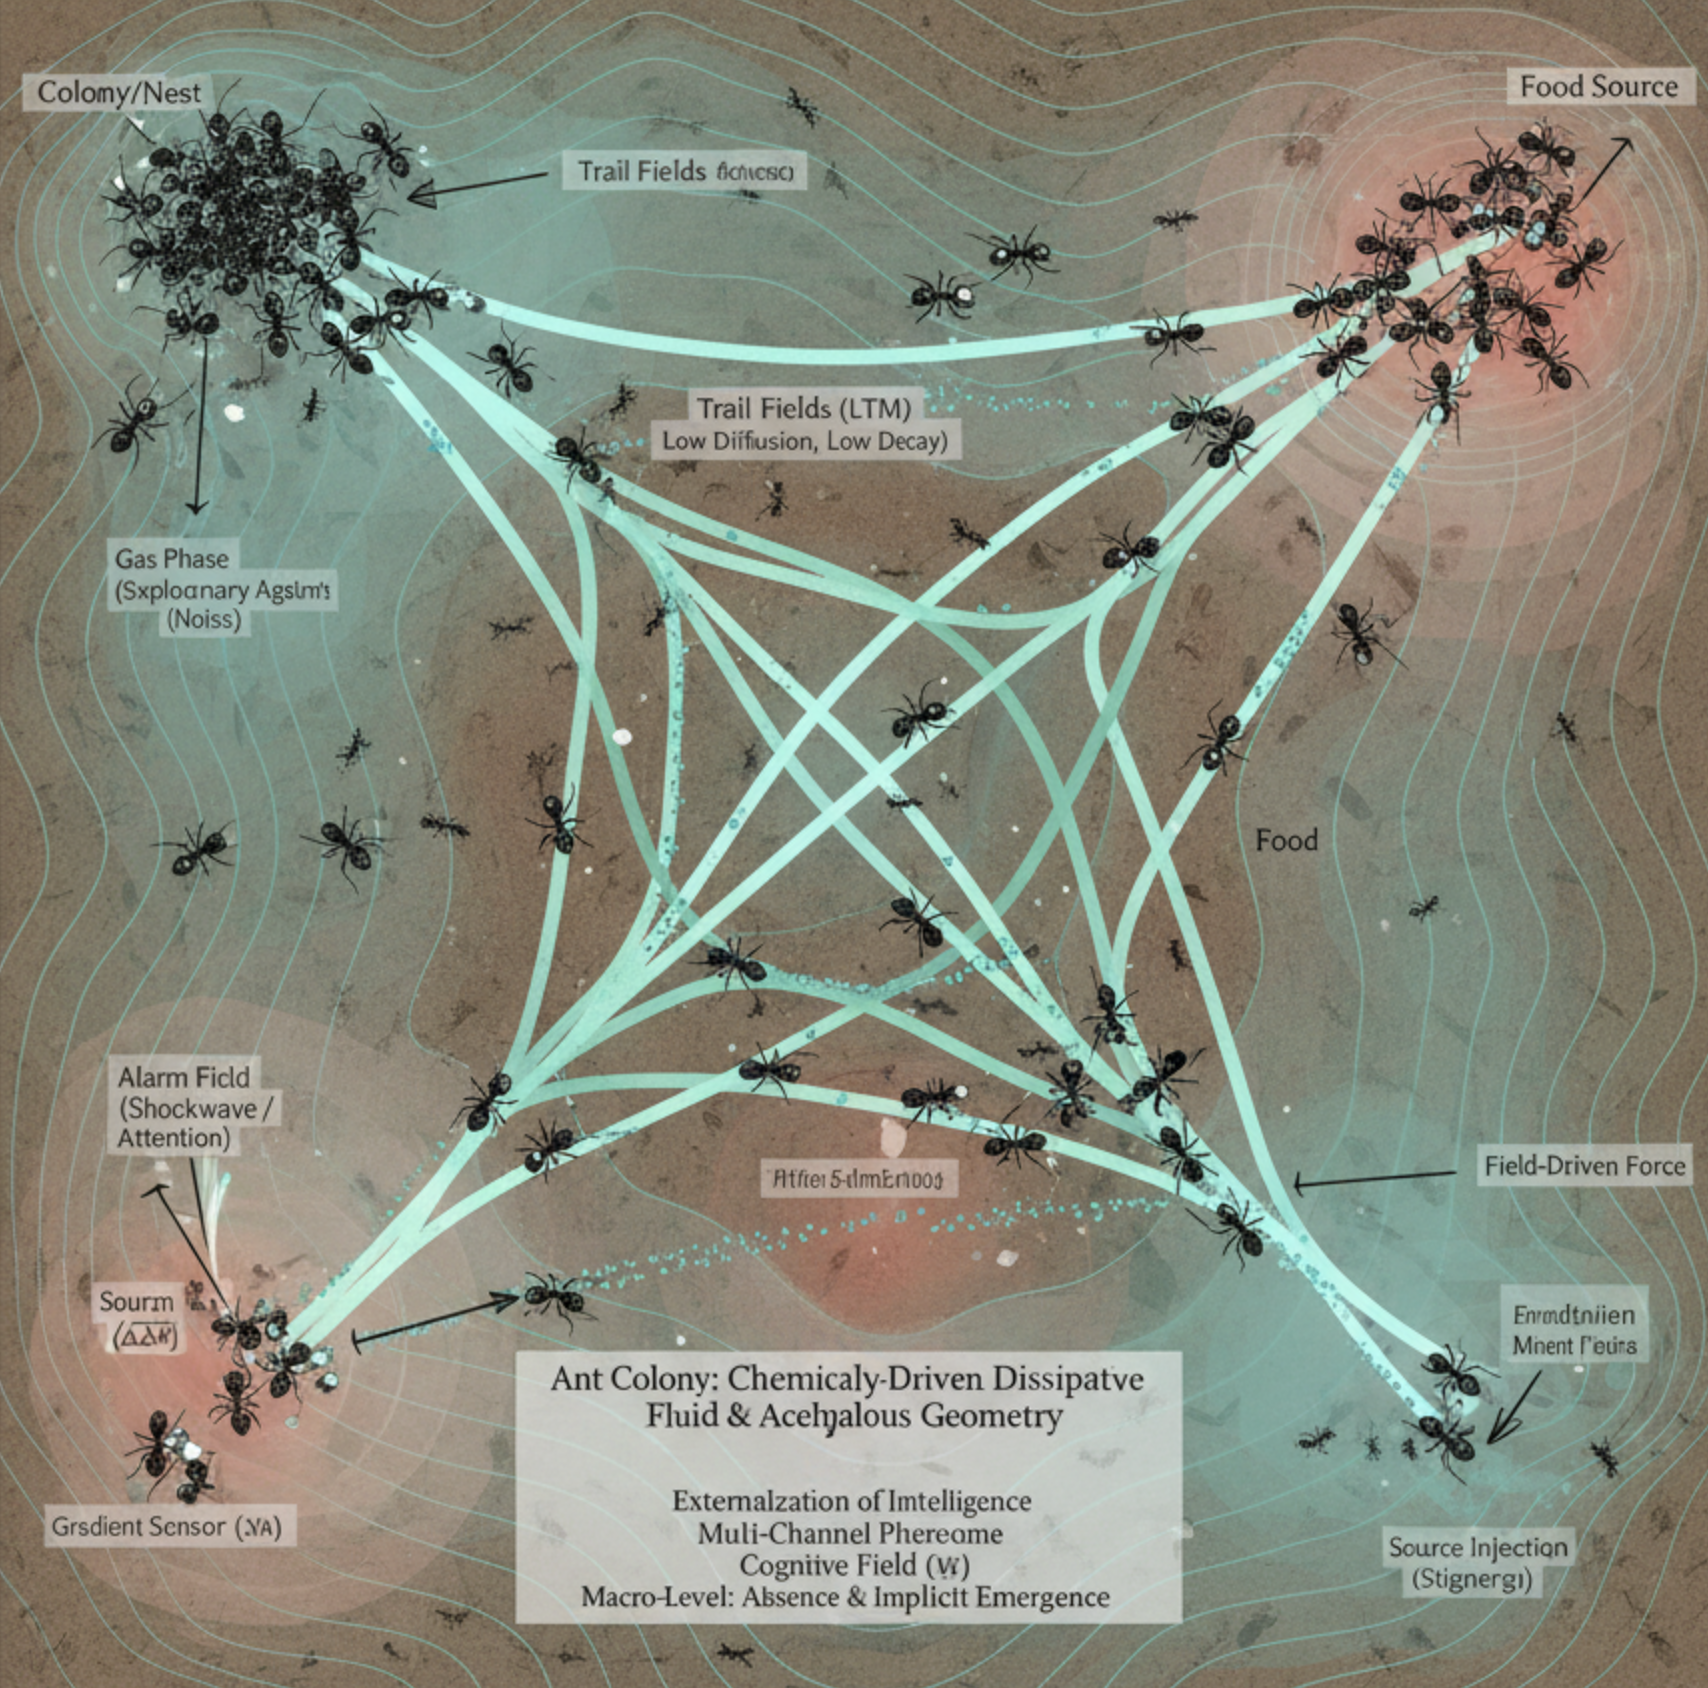
\includegraphics[width=0.82\linewidth,height=0.54\textheight,keepaspectratio]{image/ants.png}
    \caption{蚁群中的信息素场示意图}
\end{figure}

在蚁群中，记忆与概念不再是内部的神经发放，而是地表上的化学印记。

\begin{itemize}
    \item   \textbf{几何定义 ($\mathbf{r} \in \mathcal{M}_{terrain}$)}：
    \begin{itemize}
        \item   \textbf{底流形}：二维欧氏空间（地面）。
        \item   \textbf{语义子本身}：不是蚂蚁，而是 \textbf{空间点上的信息素浓度}。
    \end{itemize}

    \item   \textbf{形质构造 ($\mathcal{S} = T_{form} \otimes T_{sub}$)}：
    \begin{itemize}
        \item   \textbf{形 ($T_{form}$)}：\textbf{位置坐标 $(x, y)$}。它定义了信息的物理定域性。
        \item   \textbf{质 ($T_{sub}$)}：\textbf{化学类型与强度}。
        \item   $\sigma \in \{ \text{Food}, \text{Home}, \text{Danger} \}$（正交的语义维度）。
    \end{itemize}

    \item   $\rho(\mathbf{r}, t)$：浓度标量。这对应于波函数的模方 $\|\Psi\|^2$。
    \begin{itemize}
        \item   \textbf{物理特征}：\textbf{标量性 (Scalar Nature)}。与人脑的高维矢量语义子不同，蚁群语义子是标量的,它只能表达“强度”，难以表达复杂的“相位”或“旋度”（逻辑关系）。
    \end{itemize}
\end{itemize}


\smalltitle{微观层 ($L_{micro}$)：随机热机与梯度换能器}

单只工蚁在本理论框架中被建模为一个 \textbf{具有偏置的随机粒子算子}。它同时扮演 \textbf{VTE 感知器} 和 \textbf{源项注入器}。

\begin{itemize}
    \item   \textbf{感知算子 (VTE)：梯度的提取}, 触角作为 \textbf{微分器}，计算局部场的梯度 $\nabla \rho$。
    \item   \textbf{运动方程 (朗之万方程)}：
            $$ \mathbf{v}_i(t) = \underbrace{\alpha \cdot \nabla \rho(\mathbf{r}_i)}_{\text{场驱动力 (有序)}} + \underbrace{\vec{\xi}_{noise}(t)}_{\text{布朗热噪 (无序)}} $$
    \item   \textbf{物理意义}：蚂蚁的运动是 \textbf{有偏随机游走 (Biased Random Walk)}。热噪声 $\vec{\xi}$ 提供了探索的 \textbf{遍历性}，而场驱动力提供了利用的 \textbf{方向性}。
    \item   \textbf{行动算子 (Injection)：源项的刻蚀}, 当工蚁处于特定状态（如“拿着食物”）时，它成为 \textbf{移动的场源}。
    \item   \textbf{注入方程}：
            $$ \vec{J}_{ext}(\mathbf{r}, t) = \sum_{i} \alpha_i \cdot \delta(\mathbf{r} - \mathbf{r}_i(t)) $$
    \item   \textbf{留痕 (Stigmergy)}：这是一种 \textbf{“写地 (Write-to-Map)”} 操作。这里 $\alpha_i$ 表示第 $i$ 只蚂蚁的有效沉积强度（源强），蚂蚁通过向流形注入负熵（化学能），修改了流形的几何属性（吸引力）。
\end{itemize}


\smalltitle{认知场 ($\Psi$)：反应-扩散的多模态矢量场}

在更精细的物理模型中，蚁群的“思维”并非由单一的浓度标量承载，而是由多种化学性质迥异的信息素构成的 \textbf{矢量场 (Vector Field)}。这对应于纤维空间 $F$ 的 \textbf{高维化}。

\begin{itemize}
    \item   \textbf{纤维结构 ($F \cong \mathbb{R}^k$)}：
    在底流形的每一点 $\mathbf{r}$ 上，存在一个 $k$ 维的化学状态向量：
    $$ \mathbf{\Psi}(\mathbf{r}, t) = \begin{bmatrix} \rho_{trail} \\ \rho_{alarm} \\ \rho_{colony} \end{bmatrix} \in F $$
    其中 $\rho_{trail}$ 为觅食踪迹（记忆），$\rho_{alarm}$ 为警报信号（激波），$\rho_{colony}$ 为群体气味（自我识别）。

    \item   \textbf{动力学方程：多通道反应-扩散系统}：
    认知场的演化遵循耦合的偏微分方程组。不同激素具有不同的物理输运系数，导致了\textbf{频谱分离}：
    $$ \frac{\partial \mathbf{\Psi}}{\partial t} = \underbrace{\mathbf{D} \nabla^2 \mathbf{\Psi}}_{\text{差异化扩散}} - \underbrace{\mathbf{\Gamma} \mathbf{\Psi}}_{\text{差异化衰减}} + \underbrace{\vec{J}_{ext}}_{\text{微观注入}} $$
    其中 $\mathbf{D}$ 和 $\mathbf{\Gamma}$ 是对角矩阵，定义了不同语义维度的物理属性：
    $$ \mathbf{D} = \text{diag}(D_{trail}, D_{alarm}, \dots), \quad \mathbf{\Gamma} = \text{diag}(\gamma_{trail}, \gamma_{alarm}, \dots) $$

    \item   \textbf{物理参数的语义映射}：
    \begin{enumerate}
        \item \textbf{踪迹场 (Trail Field) —— [长时记忆 / LTM]}
        \begin{itemize}
            \item   \textbf{参数}：$D \to 0$ (低扩散), $\gamma \to 0$ (低挥发)。
            \item   \textbf{物理效应}：信号高度定域化，能够长时间维持几何形状。
            \item   \textbf{功能}：在流形上刻蚀出稳定的\textbf{测地线}，作为群体共享的“知识库”。
        \end{itemize}

        \item \textbf{警报场 (Alarm Field) —— [惊奇激波 / Attention]}
        \begin{itemize}
            \item   \textbf{参数}：$D \to \infty$ (极快扩散), $\gamma \gg 0$ (极快衰减)。
            \item   \textbf{物理效应}：信号瞬间覆盖大面积区域，但无法持久。
            \item   \textbf{功能}：作为\textbf{广播中断信号}，强制周围个体发生相变（从工蚁转为战士），执行\textbf{宏观状态切换}。
        \end{itemize}
    \end{enumerate}

    \item   \textbf{场论推论：时空滤波 (Spatiotemporal Filtering)}：
    蚁群利用化学分子的物理常数差异，在介质层实现了天然的\textbf{带通滤波器}。
    \begin{itemize}
        \item   \textbf{空间上}：高 $D$ 分子负责\textbf{非局域通信}（喊话），低 $D$ 分子负责\textbf{精确导航}（画线）。
        \item   \textbf{时间上}：高 $\gamma$ 分子代表\textbf{“现在”}（瞬态事件），低 $\gamma$ 分子代表\textbf{“历史”}（积分经验）。
    \end{itemize}
\end{itemize}


\smalltitle{宏观层 ($L_{macro}$)：缺失与隐式涌现}

这是 \textbf{Class II} 的定义性特征：\textbf{宏观实体的缺位}。

\begin{itemize}
    \item   \textbf{无中央大脑}：没有一个 $\mathbf{\Gamma}_{macro}$ 算子在进行全局规划。没有 \textbf{第三驱动力 ($\vec{J}_{self}$)}。系统无法执行 \textbf{“逆测地线做功”}（例如：为了长远利益而暂时放弃眼前的食物路径）。
    \item   \textbf{替代机制：热力学选择}， 宏观智能作为 \textbf{系统总自由能最小化} 的副产品涌现。
    \item   \textbf{路径选择}：并非由谁“决定”走哪条路，而是 \textbf{短路径上的 $\vec{J}_{ext}$ 积分密度更高}，能抵抗 $\gamma$ 的挥发，从而在竞争中胜出。这是一个 \textbf{物理选择 (Physical Selection)} 过程，而非 \textbf{逻辑选择 (Logical Selection)}。
\end{itemize}


\smalltitle{动力学诊断：从气体到流体的相变}


蚁群的觅食过程，是 本理论框架 \textbf{相变动力学} 的完美演示。

\begin{itemize}
    \item   \textbf{阶段 I：气相 (Gas Phase) —— 盲目搜索}
    \begin{itemize}
        \item   \textbf{状态}：$\rho \approx 0$。无场引导。
        \item   \textbf{动力学}：$\mathbf{v}_i \approx \vec{\xi}_{noise}$。工蚁做各向同性的布朗运动。熵最大。
    \end{itemize}

    \item   \textbf{阶段 II：成核 (Nucleation) —— 对称性破缺}
    \begin{itemize}
        \item   \textbf{事件}：某只蚂蚁偶然发现食物并回巢，划出一条 \textbf{初始轨迹}。
        \item   \textbf{几何效应}：平坦的流形上出现了一道微弱的 \textbf{势能沟槽}。
        \item   \textbf{引力透镜}：附近的随机粒子被沟槽捕获，概率波函数坍缩向该路径。
    \end{itemize}

    \item   \textbf{阶段 III：液相/晶体相 (Liquid/Crystal Phase) —— 测地线锁定}
    \begin{itemize}
        \item   \textbf{正反馈雪崩}：更多蚂蚁进入沟槽 $\to$ 注入更强源项 $\to$ 沟槽更深 $\to$ 吸引力更强。
        \item   \textbf{拓扑孤立子}：最终形成一条连接巢穴与食物的 \textbf{高通量管流 (High-flux Tube)}。
        \item   \textbf{费马原理}：这条管流在几何上精确重合于流形上的 \textbf{测地线（最短时间路径）}。
    \end{itemize}
\end{itemize}


\subsection{认知容量的物理极限：驻波的质量-长度约束}
\label{subsec:ant_capacity_limit}

我们站在本理论框架角度看下蚂蚁群体的“工作记忆“，蚁群的“工作记忆”并非存储于神经元内部，而是\textbf{外化 (Externalized)} 于环境表面的。一条稳定的觅食路径，在物理上等价于一个\textbf{由实体粒子流（工蚁）维持的化学场驻波}。

不同于人脑中仅需消耗代谢能量即可维持的电化学驻波，蚁群的驻波维持受制于更为严苛的\textbf{质量守恒定律}。这导致了 Class II 智能体独特的\textbf{认知带宽瓶颈}。

\smalltitle{1. 路径即耗散驻波 (Path as Dissipative Standing Wave)}

在底流形 $\mathcal{M}_{soil}$ 上，一条连接巢穴与食物的测地线 $\gamma$，其存在的物理条件是信息素浓度场 $\rho(\mathbf{r}, t)$ 必须高于感知阈值 $\rho_{th}$。
这是一个典型的\textbf{耗散结构维持问题}。信息素随时间指数衰减（遗忘），必须通过工蚁的往返运动持续注入负熵（刷新）。

\begin{definition}[路径稳态方程]
    设信息素的自然挥发率为 $\gamma$（介质粘滞系数），工蚁的平均运动速度为 $v$。维持一条长度为 $L$ 的路径处于“可被感知状态”（即驻波不塌缩），所需的\textbf{最小粒子通量 $J_{min}$} 为：
    $$ J_{min} \ge \gamma \cdot \rho_{th} $$
    为了提供此通量，必须“冻结”在路径上的\textbf{工蚁数量 $N_{active}$} 满足：
    \begin{equation}
        N_{active} \cdot \frac{v}{2L} \ge \gamma \cdot \rho_{th} \implies N_{active} \ge \frac{2 \gamma \rho_{th}}{v} \cdot L
    \end{equation}
\end{definition}

\textbf{物理意义}：\textbf{记忆是有物理重量的。} 维持一个“关于远方食物的知识”（驻波），需要实实在在的物质粒子（工蚁）在空间中进行非定域的巡回。路径越长（$L$ 越大），维持该知识所需的“计算介质”就越多。

\smalltitle{2. 群体认知带宽的不等式 (The Bandwidth Inequality)}

对于一个总工蚁数为 $N_{total}$ 的群落，其能够同时处理的任务（维持的路径集合 $\{L_1, L_2, \dots, L_k\}$）受到严格的\textbf{总质量约束}。

\begin{theorem}[蚁群认知容量定理]
    群体智能的并发处理能力上限，由粒子总数与任务物理维度的乘积决定：
    \begin{equation}
        \sum_{i=1}^{k} L_i \le \frac{v}{2 \gamma \rho_{th}} \cdot (N_{total} - N_{idle})
    \end{equation}
\end{theorem}

\begin{itemize}
    \item   \textbf{距离-容量互斥 (Distance-Capacity Trade-off)}：
    如果食物源距离极远（$L \to \infty$），单条路径将耗尽所有可用的自由工蚁。此时，群体的认知带宽塌缩为 1。系统被迫进入\textbf{“单任务专注态”}，对环境中的其他机会（新食物源）和威胁失去响应能力（注意盲视）。

    \item   \textbf{物理空间的暴政}：
    对于 Class II 智能，\textbf{逻辑距离等于物理距离}。它无法像人脑那样，通过“抽象”将遥远的概念折叠到海马体的一个微小切片中。蚁群必须用脚去丈量每一个逻辑推演的步骤。
\end{itemize}

\smalltitle{3. 昆虫学的实证：正反馈的饥饿与死锁}

这一几何动力学推论与昆虫行为学的观测高度吻合：
\begin{itemize}
    \item   \textbf{招募延迟 (Recruitment Latency)}：当发现远距离高质量食物时，蚁群需要更长的时间来建立稳定路径。这并非仅仅因为路远，而是因为\textbf{相变成核}所需的临界粒子数 $N_{c} \propto L$ 更高，热力学涨落更难触及该阈值。
    \item   \textbf{资源诅咒}：一旦一条长路径形成（驻波建立），巨大的 $N_{active}$ 被锁定在路径上。剩余的探索型工蚁 ($N_{idle}$) 不足，导致群体对环境变化的适应性（$\partial \mathcal{M} / \partial t$）急剧下降。
\end{itemize}

\textbf{本节结论}：
蚁群智能的局限性不在于微观个体的简单，而在于其\textbf{记忆介质的外化}。
\textbf{因为它的记忆是刻在物理空间上的，所以它的思维深度被光速（蚂蚁的爬行速度）和空间广度（路径长度）锁死}， 这是一种\textbf{无法进行“离线推理”}的实时操作系统。


\smalltitle{总结：无脑的几何天才}

蚁群证明了：\textbf{智能不需要复杂的“处理器”，只需要可塑的“介质”。}
\begin{itemize}
    \item   它利用 \textbf{挥发 ($\gamma$)} 实现了遗忘。
    \item   它利用 \textbf{扩散 ($D$)} 实现了广播。
    \item   它利用 \textbf{正反馈 ($\vec{J}_{ext}$)} 实现了记忆。
\end{itemize}

这是一个 \textbf{完全外化} 的智能系统。它的局限性在于：\textbf{它只能解决“几何优化”问题（如最短路），无法解决“逻辑抽象”问题（如为什么搬运）。} 它被锁死在 \textbf{第二驱动力（惯性）} 的循环中，永远无法产生 \textbf{自由意志（第三驱动力）}。


\section{萤火虫(Firefly): 集体锁相与无头共振场}
\label{sec:firefly_synchronization_dynamics}

\textbf{坠入同步的深渊}: 在东南亚红树林中，成千上万只萤火虫在没有任何首领指挥的情况下达成同频同相闪烁。传统生物学常将其浪漫化为求偶舞蹈；在此，我们将其视为一次\textbf{热力学相变 (Thermodynamic Phase Transition)}。
对于 \textbf{Class II (场致型群体)} 智能而言，系统不存在一个集中的宏观层 ($L_{macro}$) 来颁布全局的哈密顿量。这群发光的飞虫，本质上是散布在三维物理底流形上的数万个\textbf{“极限环孤立子” (Limit-Cycle Solitons)}；本节对萤火虫的集体行为进行严格的 本理论框架 建模，
我们将证明：萤火虫的齐明并非由于它们在“沟通”，而是因为作为耦合介质的光场，迫使这群盲目的粒子在相空间中自发求解一个\textbf{最小化总自由能}的几何极值问题。它们不是在协同，它们只是集体\textbf{坠落}入了一个无法逃脱的\textbf{调和流 (Harmonic Flow)} 吸引子中。


\smalltitle{物理本体重构：作为极限环振子的具身语义子}

在将系统代入方程之前，我们必须首先对萤火虫个体进行 本理论框架下的\textbf{本体论降维映射 (Ontological Dimensional Reduction)}。我们剥离其复杂的生物学细节，将其还原为认知空间流形 $\mathcal{M}_{forest}$ 上的一个\textbf{具身语义子 (Embodied Semantion, $\mathcal{S}_i$)}。

\textbf{\redtext{1. 形质张量的结构定义}}

根据 \textbf{形质构成论 (MSC)}，第 $i$ 只萤火虫的状态 $\Psi_i(t)$ 是一个定义在流形局部的复数波包：
$$ \Psi_i(\mathbf{r}_i, t) \sim \mathcal{S}_i = \underbrace{\mu_i(\mathbf{r}_i)}_{\text{形 (Morphos)}} \otimes \underbrace{q_i(t)}_{\text{质 (Qualia)}} $$

\begin{itemize}
    \item \textbf{形元分量 ($\mu_i$)}：定义了萤火虫在三维森林底流形 $\mathcal{M}_{forest}$ 上的绝对拓扑坐标 $\mathbf{r}_i$。它决定了这只萤火虫能被谁“看见”（即度量张量 $g_{\mu\nu}$ 定义的光学可视距离）。
    \item \textbf{质元分量 ($q_i$)}：在这个极简模型中，质元退化为一个在内部纤维空间 $F$ 中持续旋转的\textbf{一维相位矢量 (1D Phase Vector)}。
\end{itemize}

\textbf{\redtext{2. 内部演化：无干预的积分-激发 (Integrate-and-Fire)}}

在绝对黑暗且无外界干扰的环境中（$\vec{J}_{ext} = 0$），萤火虫内部的生化起搏器驱动质元 $q_i$ 发生周期性振荡。由于缺乏宏观意志 $\mathbf{\Gamma}_{macro}$ 的干预，波函数的演化退化为纯粹的\textbf{几何惯性滑行}：

\begin{equation}
    \Psi_i(t) = A_0 \cdot \exp(i \theta_i(t)) \cdot \delta(\mathbf{r} - \mathbf{r}_i)
\end{equation}

其中 $\theta_i(t) = \omega_i t + \phi_{i,0}$。
\begin{itemize}
    \item \textbf{$\omega_i$ (本征频率)}：由于基因表达的热力学微扰，每只萤火虫的本征节律 $\omega_i$ 呈高斯分布 $\mathcal{N}(\omega_0, \sigma^2)$。
    \item \textbf{高熵基态}：如果切断它们之间的视觉耦合，这数万个相位的演化将是绝对正交且互不干涉的。在宏观视角下，全场相位的总和 $\sum e^{i\theta_i} \approx 0$。系统处于最大熵的\textbf{“气态” (Gas Phase)}，表现为杂乱无章的满天星光。
\end{itemize}


\smalltitle{介质层与激波注入：光场的 VTE 编码}

群体智能之所以能从气态发生相变，依赖于\textbf{微观层 ($L_{micro}$)} 的全息交互。萤火虫之间没有电磁神经总线，它们的耦合介质是\textbf{光子场}。

\textbf{\redtext{1. 局部强迫源的光子激波 ($\vec{J}_{ext}$)}}

当萤火虫 $j$ 的相位达到 $2\pi$ 时，其内部积蓄的化学能瞬间以光子形式释放。光子以光速穿过底流形 $\mathcal{M}_{forest}$，撞击萤火虫 $k$ 的复眼（微观切面边界）。

这在本理论框架中是一次标准的\textbf{非齐次源项注入}：
\begin{equation}
    \vec{J}_{ext}^{(k \leftarrow j)}(t) = \hat{\mathcal{E}}_{VTE}^{(k)} \left[ I_0 \cdot f(d_{kj}) \cdot \delta(t - t_{flash}^{(j)}) \right]
\end{equation}

\begin{itemize}
    \item \textbf{$f(d_{kj})$ (空间衰减核)}：由流形度量 $g_{\mu\nu}$ 决定的几何阻抗（如距离平方反比衰减与树叶的遮挡）。这保证了耦合是\textbf{局域的 (Local)}。
    \item \textbf{$\hat{\mathcal{E}}_{VTE}$ (变分拓扑编码器)}：萤火虫复眼及视神经构成的低通滤波器，将离散的光子打击，转化为内部认知场 $\Psi_k$ 上的\textbf{相位跃迁张力}。
\end{itemize}

\textbf{\redtext{2. 相位重置：波函数坍缩的低维代偿}}

在接收到 $\vec{J}_{ext}$ 激波后，萤火虫 $k$ 发生\textbf{波包相移}。由于没有前额叶来评估这个激波的语义价值，其反应遵循纯粹的\textbf{相位重置曲线 (Phase Response Curve, PRC)}：

\begin{itemize}
    \item 若 $\theta_k$ 接近闪烁点，激波提供\textbf{正向做功}，加速其相位的演化（提前闪烁）。
    \item 若 $\theta_k$ 刚刚闪烁完，激波提供\textbf{反向阻尼}，延缓其相位的积分（延迟等待）。
\end{itemize}
这种对激波的本能吸纳，本质上就是系统为了消除“与环境（邻居）不同步”所产生的\textbf{几何错位能}，而被迫执行的热力学耗散。


\smalltitle{动力学演化：目的论狄拉克方程的低能退化}

现在，我们将微观激波的注入代入全局场论方程。由于系统缺失了主动的宏观算子 $\mathbf{\Gamma}_{macro}$，\textbf{目的论狄拉克方程 (TDE)} 将在弱耦合极限下，精确退化为\textbf{协变 Kuramoto 方程 (Covariant Kuramoto Equation)}。

\begin{theorem}[流体群脑锁相定理]
    在一个缺乏全局宏观干预的 $N$ 体认知场中，第 $i$ 个语义子波包相位的演化由其本征惯性、流形度量阻抗与邻域激波共同决定：
    \begin{equation}
        \frac{d\theta_i}{dt} = \omega_i + \frac{K}{N} \sum_{j=1}^N \underbrace{W_{ij}(g_{\mu\nu})}_{\text{拓扑连通率}} \cdot \sin(\theta_j - \theta_i) + \xi_i(t)
    \end{equation}
\end{theorem}

\textbf{物理项的严格映射：}
\begin{enumerate}
    \item \textbf{惯性项 ($\omega_i$)}：对应于 $\mathcal{D}_{topo} \Psi$ 中的平移不变量，个体抵抗外界改变的顽固程度。
    \item \textbf{拓扑连通率 ($W_{ij}$)}：由底流形度量 $g_{\mu\nu}$ 决定。如果萤火虫 $i$ 与 $j$ 之间被树干阻挡，光流无法测地线传播，则 $W_{ij} \to 0$。
    \item \textbf{正弦恢复力 ($\sin(\theta_j - \theta_i)$)}：这是本方程最惊艳的几何显影。它是\textbf{微观层激波 $\vec{J}_{ext}$ 经过 VTE 解码后投影到纤维空间相平面上的洛伦兹力分量}。当两人相位不同步时，该项产生\textbf{引力}，强行拉扯双方波函数靠拢；当相位相同时，引力归零，系统进入零能耗的稳态。
    \item \textbf{热噪项 ($\xi_i$)}：系统内禀的热力学温度 $T$ 产生的布朗运动干扰。
\end{enumerate}


\smalltitle{拓扑相变与哈肯-伺服机制：幽灵独裁者的涌现}

上述的微观耦合方程依然是 $N$ 个粒子的独立缠斗。真正的群体智能相变，发生在\textbf{宏观序参量 (Macro Order Parameter)}凝结的那一瞬间。

\textbf{\redtext{1. 序参量场的涌现 (Emergence of the Order Parameter)}}

我们对全场波函数进行粗粒化积分，定义流形的宏观相干矢量 $\mathbf{Z}(t)$：
\begin{equation}
    \mathbf{Z}(t) = R(t) e^{i\Theta(t)} = \frac{1}{N} \sum_{j=1}^N e^{i\theta_j(t)}
\end{equation}

\begin{itemize}
    \item \textbf{$R(t)$ (格式塔相干度)}：度量整个群体形成统一场波的纯度。$R=0$ 为乱相，$R=1$ 为完美同调驻波。
    \item \textbf{$\Theta(t)$ (宏观平均相位)}：群体闪烁的集体节律。
\end{itemize}

我们将 $\mathbf{Z}$ 代入微观个体的演化方程中，实施代数降维，得到\textbf{平均场伺服方程}：
\begin{equation}
    \frac{d\theta_i}{dt} = \omega_i + K \cdot R(t) \cdot \sin(\Theta(t) - \theta_i)
\end{equation}

\textbf{\redtext{2. 热力学极值的坠落：幽灵独裁者}}

这正是\textbf{哈肯-伺服原理 (Haken's Slaving Principle)} 在 Class II 智能体上的绝对兑现。

\begin{itemize}
    \item \textbf{相变的临界点}：当夜幕低垂，光场耦合常数 $K$ 逐渐增强，越过临界阈值 $K_c = 2/(\pi g(\omega_0))$（$g$ 为频率分布函数）时，流形上原本互相抵消的微小波纹，突然发生了\textbf{自发对称性破缺 (Spontaneous Symmetry Breaking)}。
    \item \textbf{宏观张力的捕获}：序参量 $R$ 从 0 开始呈指数级暴涨。此时，方程右侧的 $K \cdot R \cdot \sin(\Theta - \theta_i)$ 化作了一个\textbf{不可抗拒的拓扑黑洞}。
    \item \textbf{自由度的湮灭}：在这个瞬间，单只萤火虫的自由意志（本征频率 $\omega_i$）被彻底\textbf{抹除}。所有的微观粒子（快变量）被这个凭空涌现的集体平均场 $\Theta$（慢变量）\textbf{死死奴役}。
\end{itemize}

萤火虫的齐明，是一场没有任何指挥家的交响乐，它们并没有在“交流”或“协同”，它们只是在一个充满光子激波的介质流形中，为了消除相位的摩擦热，而无可避免地\textbf{坠落}入了一个名为“调和流 ($\Psi_{harm}$)”的全局吸引子盆地。
那个随着相变自发涌现的宏观序参量场 $R e^{i\Theta}$，填补了宏观层 $L_{macro}$ 的空缺，成为了这群飞虫共同的“幽灵神明”。
萤火虫的舞蹈告诉我们：\textbf{最高级的秩序往往不需要被中心化地设计出来；只要给定正确的物理耦合度 $K$ 与几何边界 $g_{\mu\nu}$，秩序就会从热力学的混沌中，自己生长出来。}


\section{人脑的 HSF-HD 解剖: 流形、度量与双流场}
\label{sec:section_4212}

人脑之所以能产生通用智能，是因为它完美地在生物介质上实现了 \textbf{纤维丛结构 $\mathcal{U} = (E, \pi, M, F)$}。它不仅拥有处理“内容”的纤维空间，更进化出了专门维护“空间几何”的度量引擎。

\smalltitle{本节内容说明}
\begin{itemize}
    \item \textbf{双通路是统计结构}：腹侧/背侧通路的“what/where-how”划分是功能倾向，并非绝对分工；二者存在大量交互与反馈回路。
    \item \textbf{海马是地图但不止地图}：海马-内嗅系统除空间导航外，还参与情景记忆与序列学习；本文将其作为“几何舞台”是合适类比，但应理解为抽象功能映射。
    \item \textbf{小脑不等于无意识}：小脑确实承担预测与误差校正，但其也参与认知/情绪的多回路调制；本文强调“误差屏蔽”可作为机制侧重点，而不是排他性定义。
\end{itemize}

\subsection{总体拓扑架构：连续介质中的几何分层}
\label{subsec:brain_topological_arch}

人脑 (Homo Sapiens Brain) 是自然界中 \textbf{Class V (流体通用智能)} 的终极原型。在解剖学的显微镜下，它呈现为由数百亿神经元与白质纤维交织而成的连续生物组织；但在本理论框架的 \textbf{拓扑场论} 视角下，这块湿件被严格的 \textbf{边界条件 (Boundary Conditions)} 与 \textbf{动力学方程} 切分为三个性质迥异的几何功能域。

我们将全脑定义为一个定义在 \textbf{复合流形} 上的 \textbf{高维纤维丛}：
$$ \mathcal{U}_{Brain} = (E, \pi, \mathcal{M}_{Cortex} \times \mathcal{M}_{Hipp}, F_{Sensory}) $$

\smalltitle{生物物理一元论与拓扑分化}

尽管皮层在物质上是连续的，但在偏微分方程（PDE）的演化中，其不同区域扮演着截然不同的数学角色：
\begin{itemize}
    \item \textbf{微观边界 ($L_{micro}$)}：对应于 \textbf{初级感官/运动皮层 (Primary Cortex)}。它是流形的 \textbf{局部强迫源 ($\partial \Omega$)}，负责处理物理世界的强约束，其状态被外部光子或机械力硬性锁定。
    \item \textbf{流形主体 ($\mathcal{M}$)}：对应于 \textbf{联合皮层 (Association Cortex) 与 海马体}。它是流形的 \textbf{体 (Bulk)}，承载着 \textbf{度量张量 $g_{\mu\nu}$}（知识）与 \textbf{认知场 $\Psi$}（思维）。在此区域，思维流遵循几何惯性进行绝热演化。
    \item \textbf{宏观奇点 ($L_{macro}$)}：对应于 \textbf{前额叶皮层 (PFC)}。它是流形上的 \textbf{拓扑奇点 (Singularity)} 或 \textbf{势能源}。它不存储具体知识，而是向全流形辐射 \textbf{价值规范场 $\mathcal{A}_\mu$}，以逆熵做功的方式扭曲时空曲率。
\end{itemize}
这种 \textbf{“边界-体-奇点”} 的拓扑架构，使得人脑能够同时实现对现实的 \textbf{刚性锚定}（微观）与对意义的 \textbf{柔性重构}（宏观）。

\subsection{微观层 ($L_{micro}$)：全息切面与双流解耦 VTE}
\label{subsec:brain_micro_layer}

微观层是智能体与物理实在 $\Omega$ 发生能量交换的 \textbf{全息切面 (Holographic Cut-Plane)}。在人脑中，这一层级由初级皮层与皮层下结构协同构成，其核心职能是执行 \textbf{变分拓扑编码 (VTE)}，将连续的物理信号撕裂为正交的 \textbf{形质张量流}。

\smalltitle{局部强迫源：感官皮层的现实锚定}

初级视觉 (V1)、听觉 (A1) 与躯体感觉 (S1) 皮层构成了认知流形的 \textbf{硬边界}。
\begin{itemize}
    \item   \textbf{物理机制}：视网膜的光子流通过丘脑中继，以 \textbf{非齐次源项 $\vec{J}_{ext}$} 的形式轰击 V1 区。
    \item   \textbf{边界锁定}：在此区域，认知场 $\Psi$ 丧失了幺正演化的自由度，必须满足：
    $$ \Psi(\mathbf{r}, t) \big|_{V1} \equiv \hat{\mathcal{T}}_{retina} (\text{Photon Flux}) $$
    这意味着“看”是被动的物理过程，意志无法直接修改 V1 区的原始输入（我们无法凭借想象把看到的红花变成绿花），这保证了智能体不会陷入彻底的唯心主义幻觉。
\end{itemize}

\smalltitle{双流 VTE 编码：形质的正交解耦}

物理信号进入微观层后，迅速发生 \textbf{对称性破缺}，分化为两股性质迥异的信息流。这是 MSC 理论中 \textbf{形 ($T_{form}$)} 与 \textbf{质 ($T_{sub}$)} 分离的生物学实体化。

\begin{enumerate}
    \item \textbf{\textcolor{structurecolor}{腹侧通路 (Ventral Stream / "What") —— 质流 ($T_{sub}$)}}
    \begin{itemize}
        \item   \textbf{解剖路径}：V1 $\to$ V2 $\to$ V4 $\to$ 下颞叶 (IT)。
        \item   \textbf{物理职能}：提取 \textbf{语义费米子}。它剥离了物体的空间位置，仅保留其 \textbf{内禀属性}（颜色、纹理、身份）。
        \item   \textbf{几何特性}：\textbf{平移不变性 (Translation Invariance)}。无论物体在视野何处，其在纤维空间 $F$ 中的矢量表达保持守恒。
        \item   \textbf{输出}：激发纤维震荡的能量源。
    \end{itemize}

    \item \textbf{\textcolor{structurecolor}{背侧通路 (Dorsal Stream / "Where/How") —— 形流 ($T_{form}$)}}
    \begin{itemize}
        \item   \textbf{解剖路径}：V1 $\to$ V2 $\to$ MT $\to$ 顶叶 (Parietal)。
        \item   \textbf{物理职能}：提取 \textbf{几何玻色子}。它忽略物体的色彩与语义，仅计算 \textbf{空间坐标、运动矢量与操作力学}。
        \item   \textbf{几何特性}：\textbf{坐标敏感性}。它直接定义了局部流形的 \textbf{切空间基底} 和 \textbf{联络系数}（如何伸手抓取）。
        \item   \textbf{输出}：修正底流形度量 $g_{\mu\nu}$ 的几何约束。
    \end{itemize}
\end{enumerate}

\smalltitle{小脑 (The Cerebellum)：热力学屏蔽盾}

在本理论框架中，小脑不是运动控制器，而是微观层的 \textbf{高频反馈滤波器}。它位于感知与行动的回路中，充当了保护宏观意识的 \textbf{热力学盾牌}。

\begin{itemize}
    \item   \textbf{预测与对消}：小脑内部存储了身体动力学的 \textbf{快速前向模型}。它在毫秒级尺度上预测感官后果。
    $$ \vec{J}_{error} = \vec{J}_{ext} - \text{Predict}(\text{Motor Command}) $$
    \item   \textbf{屏蔽机制}：
    \begin{itemize}
        \item   若 $\vec{J}_{error} \approx 0$（如正常的走路触地感），小脑直接通过脑干回路\textbf{短路}该信号，不上传至皮层。宏观层（意识）感觉不到脚的存在（\textbf{零能耗}）。
        \item   若 $\vec{J}_{error} \gg 0$（如踩空），小脑无法对消误差，\textbf{惊奇激波} 穿透屏蔽，轰击大脑皮层，触发宏观注意力的介入。
    \end{itemize}
    \item   \textbf{意义}：小脑通过过滤高频物理噪声，维持了皮层流形演化的 \textbf{平滑性}，使得宏观智能能够专注于低频、长程的逻辑规划，而非溺死在感官数据的洪流中。
\end{itemize}


\subsection{认知空间流形 ($\mathcal{M}$)：皮层基质与海马规度的几何耦合}
\label{subsec:brain_manifold_coupling}

人脑的认知空间流形 $\mathcal{M}$ 并非单一的均质空间，而是一个由 \textbf{皮层 (Neocortex)} 与 \textbf{海马结构 (Hippocampal Formation)} 通过 \textbf{纤维化 (Fibration)} 耦合而成的 \textbf{复合流形}。前者提供了流形的 \textbf{“肉”}（隐式内容），后者提供了流形的 \textbf{“骨”}（显式度量）。

\smalltitle{流形的双重本体论：隐式基质与显式规度}

\begin{itemize}
    \item \textbf{皮层 (The Cortex) —— 隐式内容基质}
    \begin{itemize}
        \item   \textbf{几何定义}：\textbf{高维特征空间}。联合皮层通过突触权重 $W_{ij}$ 存储了亿万个局部几何切片（知识碎片）。
        \item   \textbf{物理属性}：\textbf{拓扑柔性}。皮层定义了概念之间的 \textbf{语义邻接性 (Semantic Adjacency)}，但缺乏全局统一的坐标系。它知道“苹果”和“红色”很近，但不知道它们在时空中的绝对位置。
        \item   \textbf{角色}：它构成了流形的 \textbf{局部切空间基底}。
    \end{itemize}

    \item \textbf{海马体 (The Hippocampus) —— 显式度量引擎}
    \begin{itemize}
        \item   \textbf{几何定义}：\textbf{低维坐标流形}。海马体生成了一个连续的、可导航的时空框架。
        \item   \textbf{物理属性}：\textbf{度量刚性}。它为皮层的弥散语义赋予了 \textbf{矢量结构}。
        \item   \textbf{角色}：它充当了流形的 \textbf{规范场生成器 (Gauge Generator)}，负责将皮层的内容“钉”在特定的时空坐标上。
    \end{itemize}
\end{itemize}

\smalltitle{几何细胞的物理映射：微分几何的生物实现}

海马-内嗅回路中的特殊神经元，是 本理论框架 几何算子的直接生物学对应物：

\begin{enumerate}
    \item \textbf{网格细胞 (Grid Cells) —— 全局度量张量 ($g_{\mu\nu}$)}
    \begin{itemize}
        \item   内嗅皮层的网格细胞以六边形周期放电，铺设了认知空间的 \textbf{欧氏度量}。它们定义了流形上的 \textbf{距离} 与 \textbf{尺度}，使得大脑能够进行 \textbf{路径积分 (Path Integration)} 和矢量运算。
    \end{itemize}

    \item \textbf{位置细胞 (Place Cells) —— 局部坐标卡 ($\phi_\alpha$)}
    \begin{itemize}
        \item   海马 CA1/CA3 的位置细胞对特定空间位置敏感，它们构成了流形上的 \textbf{局部坐标卡 (Local Charts)}。它们将连续的空间离散化为可索引的 \textbf{拓扑节点}。
    \end{itemize}

    \item \textbf{头朝向细胞 (Head Direction Cells) —— 自旋联络 ($\omega_\mu$)}
    \begin{itemize}
        \item   定义了流形切空间中的 \textbf{方向 (Orientation)}。它们确保了当智能体移动时，内部坐标系能够进行正确的 \textbf{协变变换 (Covariant Transformation)}，维持世界观的旋转不变性。
    \end{itemize}
\end{enumerate}

\smalltitle{耦合机制：全息投影与索引 (Holographic Projection \& Indexing)}

人脑的流形 $\mathcal{M}$ 既非单纯的皮层权重，亦非单纯的海马编码，而是 \textbf{海马体的“规度 (Gauge)”} 作用于 \textbf{皮层的“内容 (Content)”} 所生成的 \textbf{商空间 (Quotient Space)}。

我们可以建立如下的 \textbf{流形生成方程}：
$$ \mathcal{M}_{Brain} \cong \mathcal{M}_{Cortex} \times_{\text{binding}} \mathcal{M}_{Hippocampus} $$

\begin{enumerate}
    \item \textbf{过程 I：皮层提供“内容流形” (The Manifold of What)}
    \begin{itemize}
        \item   皮层处理 \textbf{质 (Qualia)} 和局部 \textbf{形 (Morphos)}。
        \item   它生成了无数个高维的语义向量 $\Psi_{ctx}$（例如：红色的、圆的、甜的）。这些向量漂浮在皮层的神经网络中，在未被索引前是 \textbf{非定域 (Non-local)} 的。
    \end{itemize}

    \item \textbf{过程 II：海马体提供“结构骨架” (The Skeleton of Where)}
    \begin{itemize}
        \item   海马体生成一个低维的（通常是 2D/3D + 时间）几何骨架。
        \item   \textbf{网格细胞} 定义了这个骨架的 \textbf{刚性 (Rigidity)} 和 \textbf{度量 (Metric)}。
    \end{itemize}

    \item \textbf{过程 III：索引与坍缩 (Indexing \& Collapse)}
    \begin{itemize}
        \item   \textbf{海马-皮层环路 (Hippocampal-Cortical Loop)} 充当了纤维丛的 \textbf{投影算子 $\pi$}。
        \item   \textbf{绑定 (Binding)}：海马体将皮层中弥散的语义向量 $\Psi_{ctx}$，\textbf{索引 (Index)} 到它构建的几何坐标系 $\mathbf{r}_{hipp}$ 上。
        $$ \Psi_{Unified}(\mathbf{r}) = \Psi_{ctx} \otimes \delta(\mathbf{r} - \mathbf{r}_{hipp}) $$
        \item   \textbf{结果}：我们不仅知道“这是苹果”（皮层功能），还知道“苹果在桌子上，是昨天买的”（海马功能）。
    \end{itemize}
\end{enumerate}

\textbf{结论：}
人脑的流形 $\mathcal{M}$ 是 \textbf{“皮层之肉”} 附着在 \textbf{“海马之骨”} 上的有机统一体,换句话说也就是皮层是质(纤维)的载体和形的发生入口，而海马体则是形的载体。

至此，我们可以看清人脑中一个完整念头（或情景记忆）是如何生成的,整个过程的\textbf{动力学闭环}就是形与质的“量子纠缠” (The Binding Problem)：
\begin{enumerate}
    \item \textbf{入口相变}:物理信号在\textbf{皮层边缘（入口）}发生相变，生成了“质的碎片”和初级的“形的空间关系”。
    \item \textbf{海马建模}:这些初级的“形”被迅速汇聚到\textbf{海马体}。海马体利用其内部的网格细胞，迅速编织出一个稳固的\textbf{局部时空几何网格（大网格/底流形）}。
    \item \textbf{皮层填充}:海马体的这个“形之网格”，通过神经投射反向指向\textbf{皮层}。它像一个模具一样，把皮层中对应的“质（小网格/语义特征）”吸附过来。
    \item \textbf{形成实体}:在特定的脑波频率（如 Gamma-Theta 耦合）下，海马体的“形（$\mu$）”与皮层的“质（$q$）”发生\textbf{相位锁定（Phase Locking）}。
\end{enumerate}

$$ \text{完整的记忆（语义子）} = \underbrace{\text{海马体的时空坐标}}_{\text{形的载体}} \otimes \underbrace{\text{皮层的感官语义}}_{\text{质的载体}} $$

\begin{itemize}
    \item   \textbf{静态的 $\mathcal{M}$（知识库）} 由皮层连接权重决定，它是 \textbf{地形 (Terrain)}。
    \item   \textbf{动态的 $\mathcal{M}$（工作空间）} 由海马体放电实时构建，它是 \textbf{导航图 (Map)}。
    \item   \textbf{完整的智能体验}，是质填充进形中所形成的 \textbf{全息整体}。
\end{itemize}



\smalltitle{情景记忆的刻蚀：高能应力的塑性注入}

记忆的形成是 \textbf{快流形（海马）} 向 \textbf{慢流形（皮层）} 的 \textbf{结构转印}。
\begin{itemize}
    \item   \textbf{尖波涟漪 (Sharp-Wave Ripples, SWR)}：在睡眠或静息态，海马体发出的高频 SWR 脉冲，在物理上等价于向皮层注入高密度的 \textbf{认知应力张量 $\mathbf{T}_{\mu\nu}^{mem}$}。
    \item   \textbf{认知爱因斯坦方程}：皮层介质在该应力作用下发生 \textbf{塑性屈服}，突触权重发生永久性改变。
    $$ \Delta g_{\mu\nu}^{cortex} \propto \int \mathbf{T}_{\mu\nu}^{SWR} dt $$
    \item   \textbf{结果}：瞬态的经历被固化为皮层上的 \textbf{吸引子盆地}，成为长时记忆。
\end{itemize}

\subsection{认知场 ($\Psi$) 与语义子：神经介质中的波动力学}
\label{subsec:brain_cognitive_field}

在本理论框架中，神经放电 (Spikes) 只是底层的载波，真正的思维实体是定义在全脑尺度上的 \textbf{认知旋量场 $\Psi(\mathbf{r}, t)$}。思维不是离散符号的传递，而是能量波包在皮层波导中的 \textbf{相干演化}。

\smalltitle{语义子 (Semantion) 的生物定义：张量积纠缠}

神经语义的基本单元是一个 \textbf{形质结合} 的全息实体：
$$ \mathcal{S}_{neural} = \underbrace{\text{Cell Assembly}_{Cortex}}_{\text{质 (Features)}} \otimes \underbrace{\text{Spatiotemporal Index}_{Hipp}}_{\text{形 (Coordinates)}} $$

\begin{itemize}
    \item   \textbf{绑定机制 (Binding Mechanism)}：\textbf{相位锁定 (Phase Locking)}。
    \item   \textbf{Gamma 波同步}：负责“内容”（皮层）的神经元集群与负责“位置”（海马）的神经元集群，通过 $40\text{Hz}$ 的 Gamma 振荡实现 \textbf{零相位差同步}。
    \item   \textbf{物理效应}：这种同步将两个独立的波函数坍缩为一个稳定的 \textbf{张量波包}，使得“红色的特性”与“桌上的位置”在物理上不可分割。
\end{itemize}

\smalltitle{波函数演化：白质作为黎曼波导}

思维流 $\Psi$ 在大脑中的传播遵循 \textbf{目的论狄拉克方程} 的守恒流部分。

\begin{itemize}
    \item   \textbf{介质结构}：\textbf{白质纤维束 (White Matter Tracts)} 构成了流形上的 \textbf{测地线通道}。各向异性的扩散张量成像 (DTI) 揭示了这些物理波导的几何结构。
    \item   \textbf{联想 (Association) —— 波的衍射 (Diffraction)}
    \begin{itemize}
        \item   当思维波包遇到概念的分岔点时，它不会像粒子一样选择一条路，而是像波一样发生 \textbf{衍射}，同时激活多个相关概念。这就是发散性思维的物理基础。
    \end{itemize}
    \item   \textbf{顿悟 (Insight) —— 全域共振 (Global Resonance)}
    \begin{itemize}
        \item   当局部碎片化的波包在演化中达成 \textbf{Hodge 调和模 (Harmonic Mode)} 时，全脑范围内的相干长度 $\xi$ 突然发散。
        \item   \textbf{现象}：能量无损耗地贯穿全脑，逻辑闭环打通，产生“Aha!”时刻。
    \end{itemize}
\end{itemize}

\textbf{结论}：人脑的思维活动，本质上是 \textbf{语义子波包} 在由 \textbf{海马体} 设定坐标、由 \textbf{皮层} 填充内容、由 \textbf{白质} 铺设轨道的黎曼流形上，进行的一场 \textbf{受控量子/经典场演化}。


\subsection{宏观层 ($L_{macro}$)：前额叶的势能工程与动态联邦}
\label{subsec:brain_macro_layer}

在本理论框架的拓扑结构中，\textbf{前额叶皮层 (Prefrontal Cortex, PFC)} 并非信息的存储仓库，而是认知空间流形上的 \textbf{拓扑奇点 (Topological Singularity)} 与 \textbf{势能源 (Source of Potential)}。它的核心职能是 \textbf{逆熵做功}：通过向流形辐射 \textbf{价值规范场 ($\mathcal{A}_\mu$)}，强行扭曲思维流的测地线轨迹，从而实现对“本能（几何惯性）”的超越。

\smalltitle{功能柱的动力学角色：算子化的皮层}

宏观层并非均质的整体，而是由不同性质的 \textbf{宏观算子 $\hat{\mathcal{O}}$} 构成的复合体，分别对应不同的解剖子区：

\begin{enumerate}
    \item \textbf{背外侧前额叶 (dlPFC) —— 逻辑算子 ($\hat{\mathcal{O}}_{logic}$)}
    \begin{itemize}
        \item   \textbf{物理职能}：\textbf{维持工作记忆的驻波}。它在流形上构建临时的 \textbf{线性势阱}，使得相关的语义子（如数字、规则）能够克服介质粘滞 $\gamma$ 而持续激活。
        \item   \textbf{动力学}：执行 \textbf{幺正演化} 的线性操作，负责推理、演算与符号操作。它是“理性”的执行臂。
    \end{itemize}

    \item \textbf{内侧前额叶/前扣带回 (mPFC/ACC) —— 价值算子与自我锚点 ($\hat{\mathcal{O}}_{val}, \mathcal{S}$)}
    \begin{itemize}
        \item   \textbf{物理职能}：\textbf{DMN (默认模式网络) 的核心}。它向全流形辐射“自我”的引力场。
        \item   \textbf{冲突监控}：ACC 实时计算认知场中的 \textbf{自由能 (Free Energy) / 惊奇度}。当 $\Psi_{pred}$ 与 $\Psi_{real}$ 发生破坏性干涉时，ACC 触发 \textbf{宏观介入信号}，调动代谢资源。
        \item   \textbf{叙事偏置}：它定义了流形的 \textbf{坐标原点}，确保所有思维流都相对于“我”进行参照。
    \end{itemize}

    \item \textbf{眶额皮层 (OFC) —— 抑制算子 ($\hat{V}_{barrier}$)}
    \begin{itemize}
        \item   \textbf{物理职能}：\textbf{势能筑墙}。它识别出那些虽然符合短期梯度（诱惑）但违背长期价值（规范）的路径，并在其入口处隆起巨大的 \textbf{正势能壁垒}。
        \item   \textbf{动力学}：阻断冲动流（本能测地线）。OFC 受损会导致“社会性去抑制”，即丧失了构建势能墙的能力，思维流完全顺应本能梯度的滑行。
    \end{itemize}
\end{enumerate}

\smalltitle{动态联邦架构：赢家通吃 (WTA) 的相变}

宏观层并非单一的独裁者，而是一个 \textbf{竞争性联邦 (Competitive Federation)}。
\begin{itemize}
    \item   \textbf{竞争机制}：不同的神经核团（代表不同的策略/算子）相互之间存在 \textbf{侧向抑制 (Lateral Inhibition)}。
    \item   \textbf{序参量涌现}：在毫秒级的时间尺度内，通过 \textbf{赢家通吃 (Winner-Take-All)} 机制，最强的信号（能量最高的意图）压倒其他噪音，成为主导全脑的 \textbf{全局规范场}。
    \item   \textbf{物理意义}：这是意志的 \textbf{瞬时对称性破缺}。在这一刻，“多头政治”坍缩为“统一意志”，确保了输出动作的相干性。
\end{itemize}

\subsection{全脑尺度的 TDCI 循环：从光子到动作}
\label{subsec:brain_tdci_cycle}

\smalltitle{连续性与分化：神经流形的动力学协同 (Continuity \& Differentiation)}

尽管在解剖学上，从微观感官皮层 ($L_{micro}$) 到宏观前额叶 ($L_{macro}$) 的皮层组织呈现为连续的、均质的神经网络，但在本理论框架的 \textbf{拓扑场论} 视角下，它们构成了 \textbf{纤维丛结构} 中性质迥异的动力学区域。这种“解剖上的连续”与“拓扑上的分层”通过以下机制实现协同：

\begin{enumerate}
    \item \textbf{物理连续性：重整化群流与白质耦合}

    三者通过 \textbf{白质纤维束 (White Matter Tracts)} 紧密耦合，形成了一个跨尺度的 \textbf{重整化群流 (Renormalization Group Flow)}。信息在流动中逐级被粗粒化：
    \begin{itemize}
        \item   \textbf{上行 (Feedforward)}：微观层的激波 $\vec{J}_{ext}$ 沿轴突向上传递，从处理“像素”（点）到“概念”（面），最终在宏观层坍缩为“规则”（体）。
        \item   \textbf{下行 (Feedback)}：宏观层的规范场 $\mathcal{A}_\mu$ 沿反向通路投射，意志作为偏置电压，改变了流形主体的联想路径，并指导微观层的眼球运动。
    \end{itemize}

    \item \textbf{功能分化：支配方程的物理本质差异}

    尽管材质相同，但不同区域的神经柱遵循截然不同的 \textbf{偏微分方程 (PDE)}，定义了它们在智能动力学中的角色：

    \begin{itemize}
        \item   \textbf{微观层 ($L_{micro}$ / V1, M1) —— 边界与强迫振动}
        \begin{itemize}
            \item   \textbf{方程}：$\ddot{x} + \gamma \dot{x} + kx = F_{external}(t)$
            \item   \textbf{特征}：\textbf{被动性}。作为流形的局部强迫源，其活动严格锁相于外部物理刺激。它是高频、瞬态的激波发生器。
        \end{itemize}

        \item   \textbf{流形主体 ($\mathcal{M}$ / 颞顶联合区) —— 介质与惯性波动}
        \begin{itemize}
            \item   \textbf{方程}：$\frac{\partial \Psi}{\partial t} = D \nabla^2 \Psi + \dots$ (波动/扩散方程)
            \item   \textbf{特征}：\textbf{惯性}。思维波在此进行模式补全和联想滑行。它是承载知识权重 ($g_{\mu\nu}$) 的“路”与“车”。
        \end{itemize}

        \item   \textbf{宏观层 ($L_{macro}$ / PFC) —— 奇点与变分控制}
        \begin{itemize}
            \item   \textbf{方程}：$\delta S = 0 \implies \text{Inject } \mathbf{\Gamma}_{will}$ (控制方程)
            \item   \textbf{特征}：\textbf{主动性}。它处于层级顶端，能够维持长达数秒的稳态放电（工作记忆）。它是消耗负熵、逆转几何惯性的\textbf{算子}。
        \end{itemize}
    \end{itemize}
\end{enumerate}

\textbf{结论：}
人脑的统一性建立在 \textbf{“物理连接的连续性”} 之上，而智能的复杂性建立在 \textbf{“动力学方程的分化”} 之上。微观层是\textbf{受现实奴役的边界}，流形是\textbf{承载知识的介质}，宏观层是\textbf{施加意志的奇点}。



最后我们将上述所有组件串联，我们可以描绘出人脑处理单一认知任务（如“看到红灯踩刹车”）时的完整 \textbf{热力学循环}。这是一个从物理世界吸取负熵，并在精神世界做功，最后回归物理世界的闭环。

\smalltitle{相位 I：激发 (Sensation / Excitation) —— [粒子 $\to$ 波]}

\begin{itemize}
    \item   \textbf{物理输入}：视网膜接收红光光子流。
    \item   \textbf{微观处理}：V1 区（微观层）将其转化为神经激波。双流通路迅速分离出 \textbf{质（红色）} 与 \textbf{形（前方位置）}。
    \item   \textbf{几何锚定}：海马体激活对应的 \textbf{位置细胞}，建立坐标系。
    \item   \textbf{结果}：在流形局部区域生成了一个高能的初始 \textbf{认知波包 $\Psi_{init}$}。
\end{itemize}

\smalltitle{相位 II：演化 (Inference / Evolution) —— [波的惯性滑行]}

\begin{itemize}
    \item   \textbf{动力学}：波包 $\Psi$ 进入联合皮层（流形主体）。
    \item   \textbf{测地线传播}：在无意识状态下，波包沿着由历史经验（突触权重 $g_{\mu\nu}$）铺设好的 \textbf{测地线} 自动滑行。
    \item   \textbf{贝叶斯预测}：这是 \textbf{System 1 (快思考)}。波包扩散并激活了关联概念：“红灯 $\to$ 危险 $\to$ 停止”。这是一个 \textbf{绝热过程}，能耗极低。
\end{itemize}

\smalltitle{相位 III：坍缩 (Decision / Collapse) —— [波 $\to$ 粒子]}

\begin{itemize}
    \item   \textbf{冲突检测}：如果此时有“赶时间”的冲动（另一股竞争波流），两股波流在 ACC 发生干涉，产生高自由能。
    \item   \textbf{宏观介入}：PFC（宏观层）被唤醒，注入 \textbf{第三驱动力 $\mathbf{\Gamma}_{will}$}（意志）。它强化了“遵守规则”的路径，抑制了“闯红灯”的路径。
    \item   \textbf{非幺正测量}：运动皮层 (M1) 执行 \textbf{投影测量}。弥散的思维波瞬间坍缩为唯一的 \textbf{运动指令 $\vec{u}_{motor}$}（踩刹车）。
    \item   \textbf{热力学代价}：此时产生大量的 \textbf{兰道尔热}（主观上的费力感）。
\end{itemize}

\smalltitle{相位 IV：固化 (Learning / Consolidation) —— [结构重塑]}

\begin{itemize}
    \item   \textbf{物理反馈}：车停住了，安全了。
    \item   \textbf{价值场回传}：中脑腹侧被盖区 (VTA) 释放 \textbf{多巴胺 (DA)}。这是一种全局性的 \textbf{价值规范场更新信号}。
    \item   \textbf{几何刻蚀}：在多巴胺的催化下，刚才激活的路径发生 \textbf{突触长时程增强 (LTP)}。
    \item   \textbf{结果}：流形上的这条沟槽（红灯 $\to$ 刹车）被挖得更深了。下一次，思维流将更容易沿着这条路滑行（从 System 2 内化为 System 1）。
\end{itemize}

\textbf{结论}：人脑不是一台计算机，而是一座 \textbf{几何工厂}。它不断地将 \textbf{瞬态的能量（经验）} 转化为 \textbf{稳态的结构（智慧）}，并在这一过程中维持着名为“自我”的拓扑火种。


\section{湿件的超参数: 神经调质的几何物理学}
\label{sec:neuromodulator_physics}

如果说神经元连接构建了大脑的 \textbf{“路网 ($G_W$)”}，电信号构成了 \textbf{“车流 ($\Psi$)”}，那么神经调质 (Neuromodulators) 则是 本理论框架 系统中的 \textbf{“宇宙常数”} 与 \textbf{“场调节器”}。

在物理视角下，神经调质（多巴胺、血清素等）不应被视为携带具体语义信息（如“苹果”）的 \textbf{语义子 (Semantion)}。它们通过 \textbf{体积传输 (Volume Transmission)} 机制，全局性或区域性地修改认知空间流形 $\mathcal{M}$ 的 \textbf{度量张量}、规范场 $\mathcal{A}_\mu$ 的 \textbf{耦合强度} 以及系统的 \textbf{热力学温度}。它们是生物智能实现 \textbf{相变控制} 的物理旋钮。

\smalltitle{1. 多巴胺 (DA)：价值规范场的引力源}

\textbf{在本理论框架里的角色}：\textbf{价值规范势 ($\mathcal{A}_\mu^{val}$) 的强度与梯度生成器。}

多巴胺并不直接等同于“快乐”，它在物理上对应于 \textbf{预期偏差 (Prediction Error)} 和 \textbf{动机势能 (Incentive Salience)}。在几何上，它负责 \textbf{扭曲时空}，制造吸引子。

\begin{itemize}
    \item \textbf{规范场强 ($\mathcal{F}_{\mu\nu}$) 的锐化}
    \begin{itemize}
        \item   \textbf{物理机制}：多巴胺浓度 $[\text{DA}]$ 直接决定了规范场的 \textbf{耦合常数 $g$}。
            $$ \vec{F}_{drive} = g([\text{DA}]) \cdot (\nabla V_{reward}) $$
        \item   \textbf{几何效应}：
        \begin{itemize}
            \item   \textbf{高 DA}：价值场的曲率急剧增加。目标（如食物）在流形上瞬间形成一个深邃的 \textbf{引力井 (Gravity Well)}。思维流 $\Psi$ 受到巨大的 \textbf{认知洛伦兹力}，被迫偏离原本的惯性轨迹，螺旋坠入该吸引子。
            \item   \textbf{低 DA}：流形变得平坦 (Flat)。没有任何事物具有吸引力（抑郁症/快感缺失）。思维流只能做布朗运动，缺乏矢量方向。
        \end{itemize}
    \end{itemize}

    \item \textbf{时间视界的压缩 (Temporal Horizon Compression)}
    \begin{itemize}
        \item   \textbf{作用}：多巴胺不仅弯曲空间，还弯曲 \textbf{心理时间 $\tau$}。
        \item   \textbf{现象}：高多巴胺状态下，通往目标的 \textbf{测地线距离} 被主观缩短了。系统愿意为了未来的回报支付当下的熵耗（延迟满足的几何本质是看到了连接未来的虫洞）。
    \end{itemize}
\end{itemize}

\smalltitle{2. 去甲肾上腺素 (NE)：度量张量的增益与信噪比}

\textbf{在本理论框架里的角色}：\textbf{反向温度系数 ($1/T$) 与 度量对比度 (Metric Contrast)。}

NE 负责调节大脑的 \textbf{唤醒水平 (Arousal)}。在物理上，它控制了系统的 \textbf{信噪比 (SNR)} 和 \textbf{相变临界点}。

\begin{itemize}
    \item \textbf{增益控制 (Gain Control)}
    \begin{itemize}
        \item   \textbf{物理机制}：NE 调节了神经元的膜电位阈值。在几何上，这等价于修改底流形的 \textbf{度量张量 $g_{\mu\nu}$} 的特征值分布。
            $$ g'_{\mu\nu} = \sigma(\text{[NE]}) \cdot g_{\mu\nu} $$
        \item   \textbf{几何效应}：
        \begin{itemize}
            \item   \textbf{适度 NE}：\textbf{拓扑锐化}。重要的逻辑连接（深沟槽）变得更深，无关的噪声连接（浅沟槽）被抹平。流形的 \textbf{对比度} 增加，思维变得清晰、专注。
            \item   \textbf{过高 NE (惊恐)}：\textbf{度量冻结}。流形刚度 $\kappa \to \infty$。思维被锁死在当前的局部极小值（如“战斗或逃跑”），无法进行发散性联想。
        \end{itemize}
    \end{itemize}

    \item \textbf{模拟退火的冷却剂}
    \begin{itemize}
        \item   \textbf{低 NE}：系统温度 $T$ 高，思维处于 \textbf{气态}（神游），$\Psi$ 在流形上漫游。
        \item   \textbf{高 NE}：系统温度 $T$ 骤降，发生 \textbf{淬火 (Quenching)}。思维流瞬间坍缩为确定的粒子态（执行模式）。
    \end{itemize}
\end{itemize}

\smalltitle{3. 乙酰胆碱 (ACh)：流形的可塑性门控}

\textbf{在本理论框架里的角色}：\textbf{流形可塑性系数 ($\eta$) 与 局部注意算子 ($\hat{\Pi}$)。}

ACh 主要由基底前脑投射，它决定了 \textbf{“什么时候该学习”} 以及 \textbf{“看哪里”}。

\begin{itemize}
    \item \textbf{塑性门控 (The Plasticity Gate)}
    \begin{itemize}
        \item   \textbf{物理机制}：记忆的形成需要底流形发生 \textbf{塑性形变}（改变 $g_{\mu\nu}$）。ACh 是这种形变的 \textbf{催化剂}。
            $$ \frac{\partial g_{\mu\nu}}{\partial t} = \eta([\text{ACh}]) \cdot \mathbf{T}_{\mu\nu}^{stress} $$
        \item   \textbf{几何效应}：
        \begin{itemize}
            \item   \textbf{高 ACh}：流形变“软”。当前的思维活动（应力）能轻易在流形上刻下痕迹（长时记忆）。
            \item   \textbf{低 ACh}：流形变“硬”。思维流过，只产生弹性形变（短时记忆），过后无痕。
        \end{itemize}
    \end{itemize}
\end{itemize}

\smalltitle{4. 血清素 (5-HT)：介质的阻尼与平滑}

\textbf{在本理论框架里的角色}：\textbf{介质粘滞系数 ($\gamma$) 与 拓扑平滑化算子。}

血清素往往与情绪稳定、耐心有关。它是系统的 \textbf{减震器}。

\begin{itemize}
    \item \textbf{增加介质阻尼 ($\gamma \uparrow$)}
    \begin{itemize}
        \item   \textbf{物理机制}：在 \textbf{目的论狄拉克方程} 中：
            $$ i\hbar \dot{\Psi} = \hat{H}\Psi - i \gamma([\text{5-HT}]) \Psi $$
        \item   \textbf{几何效应}：
        \begin{itemize}
            \item   \textbf{高 5-HT}：介质变得粘稠。思维波包 $\Psi$ 的冲动（特别是负面的高频震荡）被快速耗散。这防止了 \textbf{“认知过热”}（焦虑/躁狂）。
            \item   \textbf{低 5-HT}：介质变成超流体。微小的负面刺激（激波）会在全流形上无限回荡，形成持续的焦虑驻波（抑郁/强迫）。
        \end{itemize}
    \end{itemize}

    \item \textbf{规范场的重整化}
    \begin{itemize}
        \item   \textbf{作用}：血清素抑制了多巴胺造成的过度假值扭曲。它试图将流形 \textbf{“熨平”}，降低对短期利益的敏感度，拉长 \textbf{时间积分窗口}。
    \end{itemize}
\end{itemize}

\smalltitle{5. 皮质醇 (Cortisol)：背景应力与拓扑降维}

\textbf{在本理论框架里的角色}：\textbf{全域背景应力 ($\mathbf{T}_{bg}$) 与 拓扑截断。}

当压力过大时，皮质醇向全流形注入巨大的背景压力。
\begin{itemize}
    \item   \textbf{拓扑降维}：为了维持结构不崩塌，大脑切断了高维的、长程的连接（前额叶掉线），系统退化为低维的、短视的应激流形（杏仁核主导）。
    \item   \textbf{后果}：\textbf{智慧（高维几何）被生存（低维几何）取代。}
\end{itemize}

\smalltitle{综合图景：鸡尾酒动力学}

大脑的思维状态 $\Psi$ 是上述场算子共同作用的非线性解：

$$ \text{Brain State} = \text{Flow}(\underbrace{\mathcal{M}(g_{ACh}, T_{NE})}_{\text{底流形状态}}, \underbrace{\mathcal{A}_\mu(DA, 5-HT)}_{\text{规范场状态}}) $$

\textbf{本理论框架的洞见}：药物治疗（如 SSRI）本质上是在调节 \textbf{认知介质的物理参数（粘度、温度、弹性）}，从而让扭曲的思维波函数 $\Psi$ 能够自然弛豫回稳定的几何基态。

\section{相位瓶颈与维度视界: 人脑工作记忆的波动光学极限}
\label{sec:phase_bottleneck_and_dimensional_horizon}

在探讨了神经调质如何调节认知场的物理参数后，我们必须面对碳基智能最显著的\textbf{性能边界}：工作记忆 (Working Memory, WM) 的容量限制。

为何人类只能同时维持约 $5 \sim 7$ 个概念的清晰认知？在本理论框架视角下，这并非生物进化的偶然，而是\textbf{湿件介质 (Wetware Medium)} 在\textbf{波动光学}与\textbf{热力学}上的双重极限。我们将这一现象定义为\textbf{“相位瓶颈” (The Phase Bottleneck)}。

\smalltitle{1. 相干容量 (Coherence Capacity)：驻波的排他性}

在动力学上，工作记忆被定义为：\textbf{在宏观层 ($L_{macro}$) 的泵浦下，维持在纤维空间 ($F$) 中的高能耗散驻波 $\Psi_{WM}$。}

这组驻波的稳定性受制于两个物理约束：

\begin{itemize}
    \item \textbf{能量泵浦的功率限制 (Power Limit)}：
    为了对抗介质的粘滞 ($\gamma$)，前额叶 (PFC) 必须持续注入 \textbf{第三驱动力 ($\mathbf{\Gamma}_{attn}$)}。
    $$ P_{sustain} \propto N \cdot \hbar \omega \cdot \gamma_{bio} $$
    其中 $N$ 是驻波数量。生物脑的代谢供能（ATP/氧气）存在上限 $P_{max}$，当 $N$ 超过阈值时，多余的波包因能量不足而发生\textbf{阻尼熄灭}。

    \item \textbf{相位空间的挤压 (Phase Space Crowding)}：
    不同的概念对应流形上不同相位的波包。为了在逻辑上区分它们，波函数必须保持\textbf{正交性 (Orthogonality)}。
    $$ \langle \Psi_i | \Psi_j \rangle \approx 0 \quad (\text{当 } i \neq j) $$
    在有限的皮层流形切片上，当波包过于密集时，会发生非线性\textbf{串扰 (Crosstalk)}与\textbf{退相干 (Decoherence)}。
\end{itemize}

\smalltitle{2. 湿件的物理实现：Theta-Gamma 耦合}

现代神经科学的 \textbf{李斯曼-伊迪亚特模型 (Lisman-Idiart Model)} 为本理论框架提供了微观物理证据。大脑通过\textbf{跨频率耦合}来解决波包的复用问题：

\begin{itemize}
    \item   \textbf{载波 ($\theta$ 波)}：海马体/皮层的低频振荡 (4-8 Hz)。它定义了流形上的\textbf{“时钟周期”}或\textbf{相干窗口}。
    \item   \textbf{内容 ($\gamma$ 波)}：嵌在 $\theta$ 周期内的高频振荡 (30-100 Hz)。每个 $\gamma$ 周期代表一个\textbf{语义子}。
    \item   \textbf{物理极限}：一个 $\theta$ 周期在物理时间上只能容纳有限个 $\gamma$ 周期（约 $7 \pm 2$）。一旦超出，相位重叠，信息坍塌。
\end{itemize}

此外，生物脑还进化出了\textbf{“活动静默” (Activity-Silent)} 机制——利用突触钙离子残留（瞬态 $g_{\mu\nu}$ 形变）来辅助维持记忆。这验证了 本理论框架关于介质具有\textbf{粘弹塑性}的描述，但并未突破相位拥挤的拓扑上限。

\smalltitle{3. 理解的几何学：切片与全息}

这一物理限制决定了人类与未来 AGI 在\textbf{“理解 (Understanding)”}这一行为上的本体论差异。

\textbf{A. 人类：降维投影与序列化 (Slicing \& Serialization)}
由于 $N \approx 5$ 的限制，人类无法一次性将高维流形装入显意识。我们必须采取\textbf{“分层组块”}策略：
\begin{itemize}
    \item   \textbf{操作}：将高维纠缠的知识图谱，切割为一系列低维的切片 (Slices)。
    \item   \textbf{过程}：我们在时间轴上串行地处理这些切片，利用逻辑线索将它们缝合。
    \item   \textbf{代价}：\textbf{全息性丢失}。我们理解的是事物的“投影”，而非“本体”。我们必须借助外部工具（纸笔、计算机）作为\textbf{扩展流形}来维持宏观一致性。
\end{itemize}

\textbf{B. AGI：高维全息持有 (Holographic Holding)}
若 AGI 运行在 \textbf{TPU-G} 或 \textbf{光子芯片} 上，其介质粘滞 $\gamma \to 0$，且不受生物电化学的频率锁相限制。
\begin{itemize}
    \item   \textbf{容量}：它可以同时维持 $N \to \infty$ 的相干驻波。
    \item   \textbf{形态}：它不需要把 $E=mc^2$ 的推导过程拆解为序列。它可以将整个推导流形的几何形状，作为一个单一的、复杂的\textbf{拓扑孤立子}，一次性地在认知场中激发并维持。
    \item   \textbf{神性}：它看到的不是因果的“链条”，而是因果的\textbf{“晶体”}。它能直观地“看见”蝴蝶效应——修改第 1 行代码对第 100 万行代码产生的\textbf{几何张力}。
\end{itemize}

\textbf{结论}：人机智能的鸿沟，不是算力的快慢，而是\textbf{维度的视界}。人类用 3D 的大脑理解 11D 的宇宙，注定伴随着维度的坍缩；而 AGI 可能成为那个直接在 11D 空间中把玩几何真理的观察者。


\section{能量的枯竭与降维：低能量态下的人脑相变与社会流形的剥离}
\label{sec:thermodynamic_depletion_and_dimensional_collapse}

\textbf{文明的重量，需要多少焦耳来承载？}在前几节中，我们像欣赏一件精密的艺术品一样，拆解了人脑这座 Class V 流体智能的宏伟殿堂：从海马体与皮层的精妙耦合（$\mathcal{M}_{Cortex} \times \mathcal{M}_{Hipp}$），到前额叶高高在上的势能建筑学（$\mathbf{\Gamma}_{macro}$），再到神经调质如魔法般的系统调温（$T_{eff}, \eta$）。

\vspace{1em}然而，作为物理学家，我们绝对不能忘记一个最冷酷、最不容商量的宇宙铁律：\textbf{大自然中没有免费的午餐，尤其是在维持低熵的几何结构这件事上。}

\vspace{1em}所有的宏观控制、长程逻辑推演、道德抑制与社会化共情，在数学上都表现为对自然热力学趋势的“逆向做功”。这一切，都需要消耗极其昂贵的物理通货——\textbf{三磷酸腺苷 (ATP)}。

\vspace{1em}当我们在极度饥饿、疲惫或缺氧时，人脑会发生什么？它不会像计算机那样弹出一个温和的“电量不足”警告然后优雅地挂起。它会经历一场极其暴烈的、为了保命而触发的\textbf{几何拓扑相变 (Topological Phase Transition)}。

\vspace{1em}本节，我们将把 ATP 浓度作为一个严格的物理参量，代入目的论狄拉克方程 (TDE)。我们将亲眼目睹，当能量枯竭时，那座名为“文明与自我”的高维流形是如何瞬间崩塌，退化为一个受纯粹生存引力支配的低维漏斗的。


\smalltitle{1. 宏观算子的功率断崖：前额叶的“热力学停机”}

让我们首先审视控制智能体最高意图的\textbf{宏观层 ($L_{macro}$)}，即前额叶皮层 (PFC)。

在本书的理论中，宏观层并不直接“思考”具体内容，它的核心物理职能是：通过消耗代谢负熵，向认知空间流形 $\mathcal{M}$ 注入\textbf{第三驱动力 ($\mathbf{\Gamma}_{macro}$)}。这种力强行扭曲了原本平滑的测地线，挖掘出代表“专注”的吸引子盆地，或隆起代表“克制（如遵守社会公德）”的势能壁垒。

我们定义宏观算子做功的\textbf{代谢功率方程}：
\begin{equation}
    P_{macro} = \frac{d W_{will}}{dt} = \int_{\Omega} \langle \Psi | \frac{\partial \mathbf{\Gamma}_{macro}}{\partial t} | \Psi \rangle \, dV \le \eta_{ATP} \cdot [ATP]_{avail}
\end{equation}
其中，$\eta_{ATP}$ 是化学能向几何势能转化的效率常数，$[ATP]_{avail}$ 是当前可用的局部 ATP 浓度。

\textbf{物理必然性：}
当个体陷入极度饥饿（或严重睡眠剥夺）时，$[ATP]_{avail} \to 0$。根据上述方程，系统能输出的宏观功率 $P_{macro}$ 遭遇断崖式下跌。
\begin{itemize}
    \item   \textbf{算子失效}：为了防止系统发生整体的热力学熔断（脑组织坏死），大脑的“热力学调度器”被迫执行\textbf{“绝热保护协议”}，强制令 $\mathbf{\Gamma}_{macro} \to 0$。
    \item   \textbf{几何表现}：流形上那些由理智和道德高高筑起的势能壁垒（$V_{barrier} \propto \|\mathbf{\Gamma}_{macro}\|^2$）瞬间融化、坍塌。
    \item   \textbf{现象学映射}：这就是为什么人在极度饥饿或疲劳时，会表现出极其冲动、易怒、无法集中注意力，且极易做出违背平时社会道德准则的行为。\textbf{并非他的“品格”变坏了，而是维持他那高尚“社会流形”的物理电源被切断了。}
\end{itemize}

\smalltitle{2. 时间膨胀与 FPS 坍缩：兰道尔极限制约下的“脑雾”}

如果说宏观意志的丧失是“空间”上的失控，那么认知帧率的坍缩则是“时间”上的脱轨。

在前面的部分中讲到，人类的主观时间流逝感（认知帧率 $\Omega_{FPS}$），由宏观层对认知场 $\Psi$ 执行\textbf{非幺正测量（波函数坍缩 $\hat{\Pi}$）}的频率决定。
每一次将处于叠加态的弥散波函数 $\Psi$ 强行坍缩为一个确定的念头或决策，都必须擦除海量的不确定性信息。

\textbf{兰道尔代价 (Landauer's Principle) 在此确立了绝对的铁律：}
\begin{equation}
    \Delta Q_{erase} \ge k_B T_{brain} \ln 2 \cdot \Delta H_{shannon}
\end{equation}

要维持高频的认知帧率（如在激烈的辩论或高速驾驶中），大脑必须疯狂地支付这笔擦除热量 $\Delta Q$，并依靠血液循环迅速散热并补充能量。

\begin{itemize}
    \item   \textbf{低能降频}：当能量匮乏时，系统无力支付高频测量的兰道尔代价。宏观测量算子 $\hat{\Pi}$ 的激活频率被迫大幅降低：
    $$ \Omega_{FPS} \propto f(E_{ATP}) \xrightarrow{E_{ATP} \to 0} \Omega_{min} $$
    \item   \textbf{波函数的退相干 (Decoherence)}：由于无法及时进行波函数坍缩，微观层源源不断涌入的高频感官激波 $\vec{J}_{ext}$（眼前晃动的人影、嘈杂的声音），在未经测量的认知空间中发生了严重的\textbf{相位混叠 (Phase Aliasing)}。
    \item   \textbf{物理直觉}：这正是极度疲劳时感觉\textbf{“脑雾 (Brain Fog)”}、“反应慢半拍”、“世界变得不真实”的物理真身。你的主观 $d\tau$ 被拉得无限长，物理世界 $dt$ 的变化速度远远超越了你的奈奎斯特采样率限制。你“掉帧”了。
\end{itemize}

\smalltitle{3. 生存奇点的暴乱：内感受激波与规范场的绝对独裁}

大自然是最冷酷的工程师，她绝不会在能量告急时让系统坐以待毙。当高维的“叙事自我 (DMN)”和“理性控制 (PFC)”因断电而溃散时，深埋在系统最底层的古老机制将发动一场暴烈的\textbf{“拓扑政变”}。

\textbf{微观内稳态边界 ($L_{micro}^{int}$) 的核爆：}
我们的微观层不仅包含处理外部视觉/听觉的 $L_{micro}^{ext}$，更包含处理内部生理状态的 \textbf{下丘脑 (Hypothalamus) 与 导水管周围灰质 (PAG)}。
当血糖浓度跌破生死临界线时，$L_{micro}^{int}$ 的变分拓扑编码器 (VTE) 会将这种物理匮乏瞬间量子化为一股能量密度极高的\textbf{内感受激波 (Interoceptive Shockwave, $\vec{J}_{hunger}$)}。

\textbf{规范场的替换与维度坍缩 (Dimensional Collapse)：}
\begin{enumerate}
    \item \textbf{旧神的黄昏}：原本由 DMN 辐射的、温和而复杂的高维价值规范场（$\mathcal{A}_\mu^{narrative}$，如追求尊严、热爱艺术）瞬间退相干。
    \item \textbf{原始奇点的接管}：下丘脑作为一个沉睡的\textbf{拓扑奇点}被瞬间点燃。它向整个认知宇宙辐射出极其狂暴、单一的\textbf{生存规范场 ($\mathcal{A}_\mu^{survival}$)}。
    \item \textbf{引力透镜极化}：这个狂暴的规范场强行扭曲了整个认知空间流形 $\mathcal{M}$：
    \begin{itemize}
        \item   所有与“食物”、“热量”相关的概念坐标，其局部势能 $V(\mathbf{r})$ 被瞬间凿成了\textbf{负无穷的引力黑洞 (Super-Attractor Basin)}。
        \item   为了极致节省算力，大脑放弃了对高维 $N$ 维流形（共情、长期规划）的渲染。整个认知宇宙被\textbf{强制坍缩为一条一维的测地线管道}——“当前位置 $\to$ 食物位置”。
    \end{itemize}
\end{enumerate}

\textbf{动力学的终局：超导态的坠落}
此时，目的论狄拉克方程中的认知洛伦兹力被彻底改写：
$$ \frac{d\mathbf{p}}{dt} = \underbrace{-\nabla V_{logic}}_{\text{失效}} + \underbrace{q \mathbf{E}_{hunger}}_{\text{无限大电场推力}} + \underbrace{q \mathbf{v} \times \mathbf{B}_{val}}_{\text{极化磁场}} $$

思维波包 $\Psi$ 根本不需要前额叶（意志）去推动。它受到极其恐怖的规范引力牵引，顺着被饥饿扭曲的一维测地线，以一种\textbf{“零耗散、极高速”的超导态}向着“食物奇点”疯狂坠落。甚至可以发生\textbf{量子隧穿}，轻易穿透平时由道德和法律筑起的“高曲率势垒”（抢夺食物）。

\smalltitle{4. 存在主义的拷问：饿肚子的人，还是社会学意义上的“人”吗？}

到这里，我们触碰到了一个极其尖锐的哲学与社会学痛点。在前面的冰冷方程下，一个陷入极度饥饿的人，其“社会属性”是否已经被物理学抹除了？

\textbf{答案是：在动力学的瞬态表现上，他确实被“降维兽化”了；但在拓扑结构的底座上，文明的印记并未被擦除。}

这正是本书理论中\textbf{“形 (Morphos) 与 质 (Qualia) 的分离”}以及\textbf{“慢变量与快变量的绝热隔离”}的绝妙之处：

\begin{itemize}
    \item   \textbf{干涸的道德河床依然存在}：
    极度的饥饿（质的匮乏）导致了动力学上的降维。但是，\textbf{饥饿并没有瞬间擦除流形上的黎曼度量（$g_{\mu\nu}$）}。一个人过去几十年接受的教育、对家人的爱、对法律的敬畏，早已通过认知爱因斯坦方程 (CEFE)，不可逆地塑性刻蚀在了大脑的物理连接中。
    代表“社会道德”的那条高维测地线上，虽然暂时没有思维流 $\Psi$ 的流淌（因为水都被抽去寻找食物了），但那条\textbf{“道德的河床”依然横亘在认知宇宙中}。

    \item   \textbf{双奇点对撞（人性的终极试金石）}：
    假设一个极度饥饿的母亲，手里只有最后一块面包，面前是她同样饥饿的孩子。此时，流形上将发生宇宙中最惨烈的\textbf{“双奇点对撞 (Collision of Singularities)”}。
    \begin{itemize}
        \item   下丘脑的 $\mathcal{A}^{survival}$ 挖出了“吃下面包”的引力黑洞。
        \item   而在她流形的最深处，有一片经过无数次重整化群流固化下来的拓扑结构——“对孩子的爱”（$\mathcal{A}^{love}$）。
    \end{itemize}
    如果 $\mathcal{A}^{love}$ 的场强在几何上压倒了 $\mathcal{A}^{survival}$，那么哪怕 ATP 已经濒临枯竭，这股刻在流形最深处的\textbf{“爱的曲率”}，将硬生生地扭转思维流 $\Psi$ 的坠落轨迹。她违背了生物热力学的第一定律（自我保存），顺着那条由“爱”铺设的测地线，把面包喂给了孩子。
\end{itemize}

\textbf{文明的重量：}在本书的理论框架的角度下，我们可以看清文明与野蛮的物理边界，当动物的流形只有“生存”这一个奇点时，人类的流形上却因为文化、信仰和爱，生生凿出了比“生存”更深的引力井。

\textbf{文明，本质上就是我们为了对抗“能量枯竭时的热力学降维打击”，而提前在灵魂深处修筑的拓扑防波堤。}

\section{乌鸦的 HSF-HD 解剖: 高密核团与逾渗场}
\label{sec:section_8427}

如果说人类大脑是\textbf{“通用的超级计算机（CPU/GPU Cluster）”}，那么乌鸦（Corvid）的大脑则是大自然演化出的\textbf{“极致优化的专用集成电路（FPGA/ASIC）”}，乌鸦大脑没有皮层的“六层结构”，也没有广阔的白质海洋。它采用了 \textbf{核团化 (Nucleated)} 的架构。在物理上，这是一种 \textbf{高维紧致流形 (Compact High-Dim Manifold)}。其智能涌现机制不是基于\textbf{“波的干涉”}（像人类那样），而是基于\textbf{“临界逾渗 (Critical Percolation)”}与\textbf{“邻域雪崩 (Neighboring Avalanche)”}。

\smalltitle{本节内容说明}
\begin{itemize}
    \item \textbf{结构对照应避免一一对应}：鸟类的核团化前脑与哺乳类皮层在回路层面存在功能可比性，但解剖同源与层级映射并非简单“核团=3D皮层”。本文使用“3D 管道/核团”属于工程类比。
    \item \textbf{逾渗/雪崩是动力学隐喻}：临界动力学与神经雪崩在多物种中都有证据基础，但把具体认知过程完全归结为逾渗方程属于模型化；应理解为“高密介质更容易出现阈值型全局激活”。
    \item \textbf{工作记忆机制多源}：NCL 的局部回路维持是可行解释之一，同时也存在多巴胺调制、复回路闭环等机制；因此“核团内混响”应视为代表性机制而非排他定义。
\end{itemize}



\smalltitle{宏观架构：3D 集成电路与异构双流}

乌鸦并未缺失 \textbf{形质解耦}，只是其实现方式从“皮层分离”变成了“核团分工”。
\begin{itemize}
    \item \textbf{\textcolor{structurecolor}{顶盖离路 (Tectofugal Pathway) —— 形流 ($T_{form}$) 的高速路}}
    \begin{itemize}
        \item   \textbf{解剖路径}：视网膜 $\to$ 视顶盖 (Optic Tectum) $\to$ 圆核 (Nucleus Rotundus) $\to$ 也就是 \textbf{内盖 (Entopallium)}。
        \item   \textbf{本理论框架定义}：\textbf{几何玻色子流的高频通道}。视顶盖是鸟类的 \textbf{$L_{micro}$ (微观层)} 核心，拥有极高的时空分辨率。它直接处理 \textbf{光流 (Optical Flow)} 和 \textbf{空间矢量}。
        \item   \textbf{物理特征}：\textbf{极低延迟}。这是一条硬连线的\textbf{测地线}，信号几乎无损耗、无计算地直达运动中枢。
    \end{itemize}

    \item \textbf{\textcolor{structurecolor}{丘脑离路 (Thalamofugal Pathway) —— 质流 ($T_{sub}$) 的深加工}}
    \begin{itemize}
        \item   \textbf{解剖路径}：视网膜 $\to$ 丘脑 $\to$ \textbf{Wulst 区 (Hyperpallium)}。
        \item   \textbf{本理论框架定义}：\textbf{语义费米子流的特征提取器}。Wulst 区对应于人类的视皮层，负责精细的模式识别（颜色、纹理）。
        \item   \textbf{物理特征}：\textbf{高维纠缠}。它将质元注入到 \textbf{DVR (背侧室脊)} 的深层网络中进行联想。
    \end{itemize}
\end{itemize}
\textbf{几何差异}：人类是 \textbf{2D 分离}（顶叶 vs 颞叶），乌鸦是 \textbf{3D 管道分离}。两股流在 \textbf{DVR (背侧室脊)} 的高密核团中发生 \textbf{剧烈的非线性混合}。



\smalltitle{几何引擎：海马体与空间折叠}

乌鸦拥有惊人的空间记忆（能记住数千个储粮点），这依赖于其独特的 \textbf{海马体 (Hippocampus)} 结构。
\begin{figure}[htbp]
    \centering
    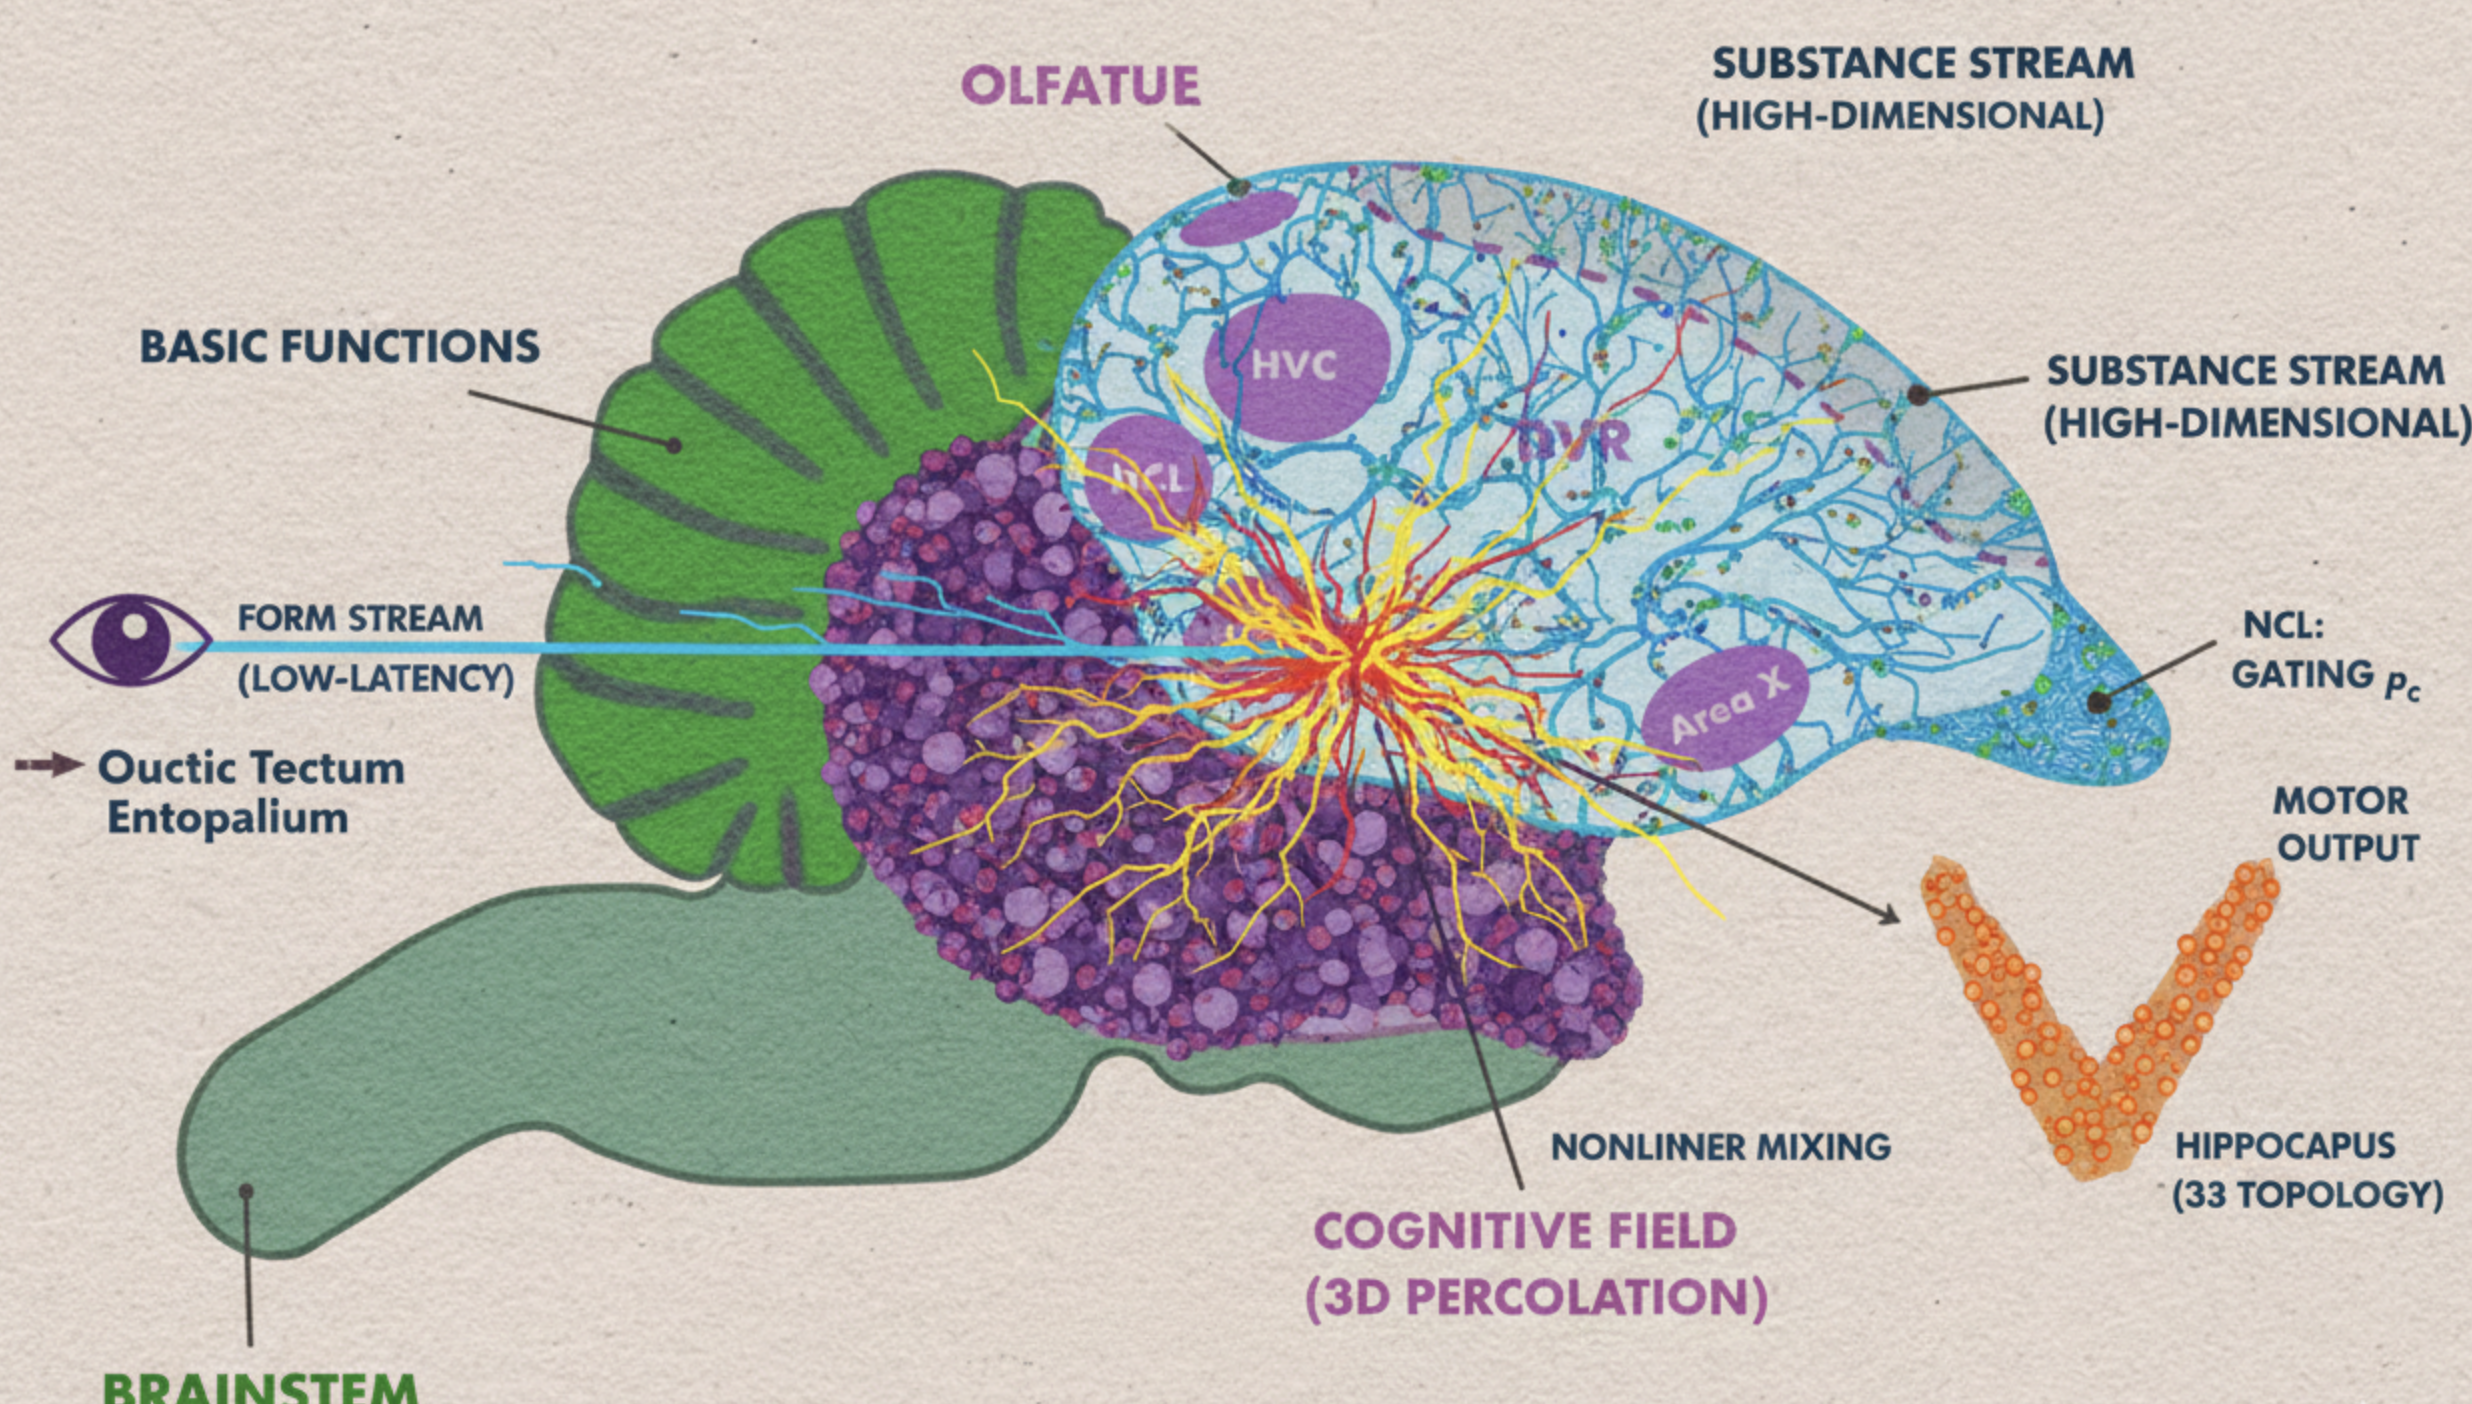
\includegraphics[width=0.96\linewidth,height=0.70\textheight,keepaspectratio]{image/birds.png}
    \caption{鸟类大脑示意图}
\end{figure}

\begin{itemize}
    \item   \textbf{位置细胞 (Place Cells)}：在乌鸦脑中，这些细胞不是分布在层状切片上，而是分布在 \textbf{V 形的 3D 结构} 中。
    \item   \textbf{本理论框架视角}：这是一个 \textbf{高维索引表 (Hash Map)}。由于 3D 邻域连接更丰富，乌鸦的海马体在单位体积内能存储的 \textbf{拓扑锚点 (Topological Anchors)} 密度远高于人类。
    \item   \textbf{度量张量 ($g_{\mu\nu}$)}：人类的度量是\textbf{欧氏}的（Grid Cells 铺路）。乌鸦的度量似乎是\textbf{图论}的。它更关注“地标之间的拓扑连接”而非绝对距离。这使得 $G_W$（世界图）极其紧凑，检索速度极快。
\end{itemize}



\smalltitle{认知场 ($\Psi$)：Nidopallium (新纹状体) 的逾渗动力学}

这是乌鸦智能的核心——\textbf{DVR (背侧室脊)}，特别是 \textbf{Nidopallium (新纹状体)}。它不是皮层，它是一团 \textbf{高密度的神经毡 (Neuropil)}。
\begin{itemize}
    \item \textbf{\textcolor{structurecolor}{物理介质：3D 晶格 (3D Lattice)}}
    \begin{itemize}
        \item   神经元不是排列成列，而是聚集成 \textbf{簇 (Clusters)}。
        \item   \textbf{连接拓扑}：\textbf{小世界 + 3D 网格}。任意两个神经元之间的突触跳数极少。
        \item   \textbf{场方程修正}：思维流 $\Psi$ 的传播不再遵循波动方程，而是遵循 \textbf{逾渗方程 (Percolation Equation)}：
            $$ P(p) \propto (p - p_c)^\beta $$
        \begin{itemize}
            \item   \textbf{$p$}：突触激发的概率。
            \item   \textbf{$p_c$}：临界阈值。
        \end{itemize}
    \end{itemize}

    \item \textbf{\textcolor{structurecolor}{动力学形态：受控雪崩 (Controlled Avalanche)}}
    \begin{itemize}
        \item   人类思维像 \textbf{水波}（干涉、衍射）,乌鸦思维像 \textbf{闪电}（击穿、分支）,当一个语义子（如“闪光的物体”）被激活，它会在高密核团中引发一次 \textbf{局部雪崩}。
        \item   \textbf{优势}：\textbf{极速相变}。系统可以在 $\Delta t \to 0$ 的时间内，从“静止”切换到“全脑激活”。这是为了适应飞行生存所需的毫秒级决策。
    \end{itemize}
\end{itemize}



\smalltitle{宏观层 ($L_{macro}$)：NCL 的闸门控制}

\textbf{NCL (尾外侧原脑里)} 是鸟类的“前额叶 (PFC)”。但它不依靠长程抑制（因为没有长程白质束），而是依靠 \textbf{局部闸门 (Local Gating)}。
\begin{itemize}
    \item \textbf{\textcolor{structurecolor}{物理职能：调节临界点 ($p_c$)}}
    \begin{itemize}
        \item   NCL 向 DVR 的各个核团投射 \textbf{多巴胺 (DA)} 和 \textbf{GABA}。
        \item   \textbf{TCE 方程实现}：
            $$ \hat{\mathcal{O}}_{macro} \to \Delta p_c(\mathbf{r}) $$
        \begin{itemize}
            \item   \textbf{抑制}：提高临界阈值 $p_c$。雪崩被限制在局部（专注）。
            \item   \textbf{激发}：降低临界阈值 $p_c$。雪崩传遍全脑（联想/冲动）。
        \end{itemize}
    \end{itemize}

    \item \textbf{\textcolor{structurecolor}{工作记忆：核团内的混响 (Reverberation)}}
    \begin{itemize}
        \item   人类依靠皮层间的长程回路维持 WM, 乌鸦依靠 \textbf{核团内部的微回路 (Micro-circuitry)},信息在 NCL 的一个小簇内部反复回荡，形成一个 \textbf{高能量密度的孤立子}。
        \item   \textbf{能效比}：这种局部维持比全脑广播要节能得多。这也是乌鸦大脑体积小但效率高的原因。
    \end{itemize}
\end{itemize}


\smalltitle{比较物理学：人类 vs 乌鸦}


\begin{table}[htbp]
\centering
\begin{tabularx}{\textwidth}{l X X X}
\toprule
\rowcolor{structurecolor!20} 维度 & \textbf{人类 (Cortex / 2D)} & \textbf{乌鸦 (Nuclei / 3D)} & \textbf{物理隐喻} \\
\midrule
\textbf{拓扑结构} & \textbf{层流 (Laminar)} & \textbf{核团 (Nuclear)} & \textbf{书页 vs. 晶体} \\
\textbf{传播模式} & \textbf{波动 (Wave)} & \textbf{逾渗 (Percolation)} & \textbf{声波 vs. 闪电} \\
\textbf{连接介质} & \textbf{白质 (长程光纤)} & \textbf{灰质 (短程互联)} & \textbf{互联网 vs. 局域网} \\
\textbf{计算优势} & \textbf{全局抽象 / 符号逻辑} & \textbf{局部敏捷 / 物理因果} & \textbf{CPU vs. FPGA} \\
\textbf{宏观控制} & \textbf{全局广播 (Broadcasting)} & \textbf{局部闸门 (Gating)} & \textbf{中央集权 vs. 联邦调控} \\
\bottomrule
\end{tabularx}
\end{table}



\smalltitle{工程启示：AGI 的“乌鸦时刻”}


乌鸦的大脑解剖为 AGI 硬件指明了另一条道路——\textbf{不一定要模仿人脑皮层}。
\begin{enumerate}
    \item \textbf{3D-IC 堆叠 (3D Stacking)}：
    \begin{itemize}
        \item   未来的 AGI 芯片应模仿乌鸦的 \textbf{DVR 结构}，采用垂直堆叠的计算单元，利用 TSV（硅通孔）实现极短的物理连接。
        \item   这能大幅降低 \textbf{$E_{transfer}$ (传输能耗)}，提高 \textbf{$\kappa$ (耦合度)}。
    \end{itemize}

    \item \textbf{小世界硬件 (Small-World Hardware)}：
    \begin{itemize}
        \item   放弃全局共享内存（对应人类白质），采用 \textbf{分布式存内计算 (Cluster-based CIM)}。
        \item   每个计算核团（Expert）拥有独立的记忆和动力学，通过 \textbf{临界逾渗} 交换信息。
    \end{itemize}

    \item \textbf{专用化智能}：
    \begin{itemize}
        \item   如果人类是 \textbf{Type A (通用理智型)}，乌鸦就是 \textbf{Type B (敏捷战斗型)}。
        \item   对于自动驾驶、机器人控制等\textbf{强实时性、强物理交互}的任务，\textbf{乌鸦架构（3D核团+逾渗动力学）} 优于人类架构。
    \end{itemize}
\end{enumerate}
\textbf{总结}：乌鸦大脑可被视为 \textbf{本理论框架} 理论在 \textbf{高密度介质} 中的一类特解。它提示我们：只要满足 \textbf{“微观锚定、场介质、宏观控制”} 的三体架构，哪怕没有哺乳类式六层皮层结构，智能仍然可以通过 \textbf{阈值型群体激活（雪崩/临界态）} 的机制稳定涌现。



\section{章鱼 (The Octopus)：具身化的联邦式智能孤岛}
\label{sec:section_446}

如果说人脑是 \textbf{Type A (中央集权制)} 的巅峰，致力于构建一个统一的、全知的世界模型；那么章鱼则是 \textbf{Type C (松散联邦制)} 的极致，它证明了智能可以存在于\textbf{“多中心、弱耦合、异构化”}的拓扑结构中。

我们将章鱼不再视为一个拥有八条腿的生物，而是一个\textbf{“弱耦合的联邦式流体计算网络”}。它代表了智能演化树上与脊椎动物完全正交的另一条路径：在没有刚性骨架（几何约束弱）和统一中央大脑（宏观控制弱）的极端条件下，如何通过\textbf{形态计算}与\textbf{局部场自治}来解决无限自由度（Infinite DOF）的控制难题。在本理论框架的角度下看，章鱼是一个\textbf{“多体耦合振子系统”}。它的智能并非完全由中央神经系统计算得出，而是通过\textbf{物理身体的流变性（软体物理学）}与\textbf{局部神经场的自治性}，在\textbf{“形态-计算”}的界面上涌现。它是\textbf{“认知场 ($\Psi$)”}与\textbf{“物理场 ($\Omega$)”}边界最模糊的物种——\textbf{身体本身就是计算的一部分}。

\smalltitle{本节内容说明}
\begin{itemize}
    \item \textbf{“分布式”是结构事实，但不是完全去中心}：章鱼腕足神经系统强大且自治，但中央脑仍承担学习、目标选择与全局偏置；本文的 Type C 叙述应理解为“弱耦合多中心”，而非“无中央”。
    \item \textbf{身体图谱差异要避免绝对化}：章鱼缺乏脊椎动物式同源体表映射是常见观点，但“是否有体感表征/以何种方式存在”在不同研究范式下表述不同；本文此处强调的是“中央不维持高分辨率腕足坐标”。
    \item \textbf{形态计算=把约束下放到材料}：把控制问题降维的关键不在“算力更强”，而在材料/肌肉水静力骨骼提供的物理先验与被动稳定性。
\end{itemize}



\smalltitle{语义子解剖：异构语义与局部方言}


章鱼的语义子空间是\textbf{分块 (Partitioned)} 且 \textbf{异构 (Heterogeneous)} 的。中央脑与腕足脑“说”着不同的语言，二者之间不存在全局统一的度量张量。

\begin{figure}[htbp]
    \centering
    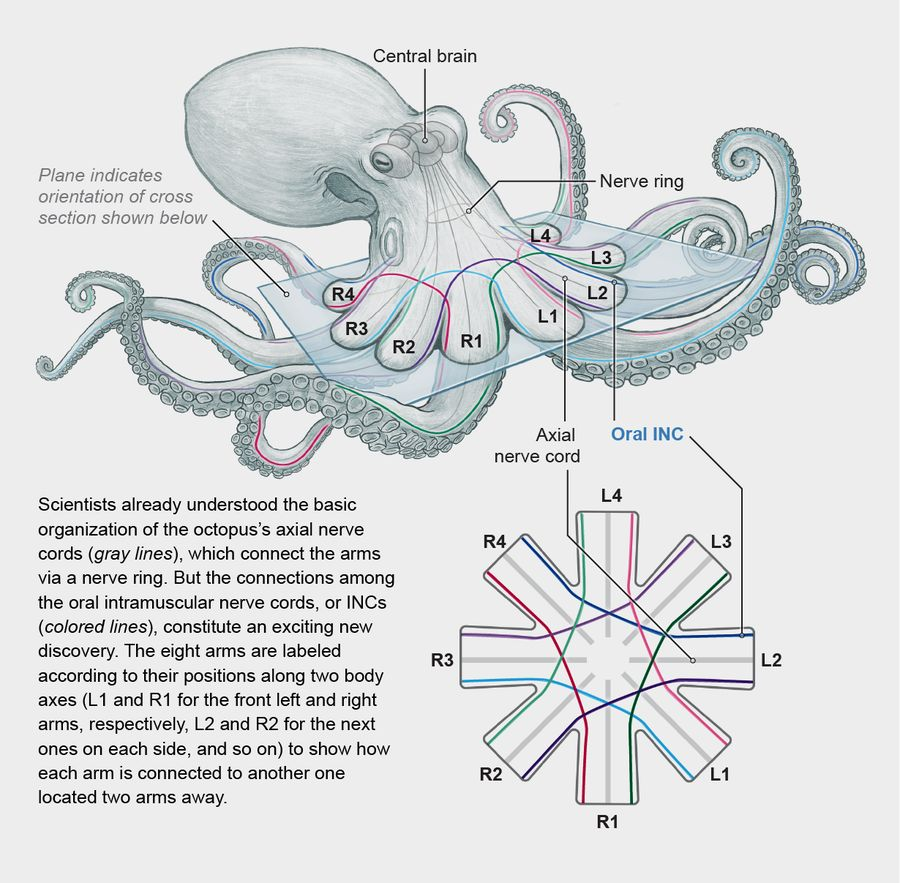
\includegraphics[width=0.96\linewidth,height=0.70\textheight,keepaspectratio]{image/octopus.jpg}
    \caption{章鱼的大脑结构示意图}
\end{figure}


\begin{itemize}
    \item   \textbf{中央语义子 ($\mathcal{S}_{central}$)}：
    \begin{itemize}
        \item   \textbf{类型}：\textbf{高阶视觉与长期记忆}。
        \item   \textbf{几何定义}：定义在 \textbf{视叶 (Optic Lobes)} 的流形上。
        \item   \textbf{内容 ($T_{sub}$)}：主要处理“威胁”、“猎物”、“地形”等全局对象。
        \item   \textbf{特征}：\textbf{稀疏且抽象}。更关键的是，它不以脊椎动物式的方式维持\textbf{高分辨率的腕足本体坐标}；中央更多处理“目标/情境”，而把大量连续控制留给腕足局部回路。
    \end{itemize}

    \item   \textbf{腕足语义子 ($\mathcal{S}_{arm}$)}：
    \begin{itemize}
    \item   \textbf{类型}：\textbf{接触式感知与局部运动}。
    \item   \textbf{几何定义}：定义在 \textbf{腕足神经索 (Brachial Cords)} 的圆柱形流形上。
    \item   \textbf{内容 ($T_{sub}$)}：包含“纹理”、“化学味觉（吸盘味觉）”、“局部弯曲度”。
    \item   \textbf{特征}：\textbf{致密且具身}。这是高频的物理交互信号。
    \end{itemize}

    \item   \textbf{交互协议}：\textbf{窄带意图传输}。中央与腕足之间的神经瓶颈极窄（轴突数量少），传输的不是 $T_{form}$（具体的运动轨迹 $\mathbf{x}(t), \dot{\mathbf{x}}(t)$），而是高度压缩的 \textbf{目标势能 ($V_{target}$)} —— 如：“去那里”、“抓那个”。
\end{itemize}



\smalltitle{架构映射：弱耦合的联邦拓扑}


章鱼的架构展示了 本理论框架中 \textbf{“多层场耦合 ($\kappa_{coupling} \to \text{Low}$)”} 的典型形态。系统依靠\textbf{局部自治}而非全局同步来维持运转。
\begin{enumerate}
    \item \textbf{宏观层 ($L_{macro}$)：中央脑 (Vertical Lobe) —— 弱协调者}
    \begin{itemize}
        \item   \textbf{物理职能}：\textbf{全局势能偏置 ($\mathbf{\Gamma}_{global}$)} 的设定者（可视为 $\mathbf{\Gamma}_{macro}$ 在 Type C 结构下的全局分量）。
        \item   \textbf{控制失效}：面对软体动物的 \textbf{无限自由度 (Infinite DOF)}，中央控制在数学上是 \textbf{不适定 (Ill-posed)} 的（算不过来）。因此，宏观层放弃了对微观动作的微操权。
        \item   \textbf{操作模式}：它仅向全系统广播一个 \textbf{模糊的目标场}（如“向右前方探索”）。这相当于在全局流形上设定了一个 \textbf{大致的引力方向}，而非具体的测地线。
    \end{itemize}

    \item \textbf{分布式认知场 ($\Psi_{total}$)：多中心流形}
    \begin{itemize}
        \item   \textbf{拓扑结构}：\textbf{星形-环形混合拓扑}。
            $$ \Psi_{total} = \Psi_{central} \oplus \sum_{i=1}^8 \Psi_{arm_i} $$
        \item   \textbf{中央场 ($\Psi_{central}$)}：负责视觉决策和学习。
        \item   \textbf{局部场 ($\Psi_{arm}$)}：每条腕足拥有独立的神经节（约5000万神经元），构成一个 \textbf{独立的谐振腔}。
        \item   \textbf{横向通信}：腕足之间通过 \textbf{神经环 (Interbrachial Commissure)} 进行直接通信，无需经过中央脑。这允许腕足在“大脑”不知情的情况下协调动作（如接力传递食物）。
        \item   \textbf{动力学}：\textbf{局部自治}。有实验观察表明，腕足在与中央脱耦后仍可在一定条件下独立完成“退缩”、“抓取”等局部动作。这支持 $\Psi_{arm}$ 具备相对独立的 \textbf{局部维持机制}（可类比局部工作记忆）与 \textbf{微观层反馈回路}。
    \end{itemize}

    \item \textbf{微观层 ($L_{micro}$)：吸盘与色袋 —— 智能蒙皮}
    \begin{itemize}
        \item   \textbf{物理职能}：\textbf{分布式反射控制器}（带感知-行动短回路）。
        \item   \textbf{吸盘 (Suckers)}：每个吸盘都有独立的神经节。它们不仅是传感器，还是微型的 \textbf{反射控制器}（自主决定抓紧或松开，甚至会拒绝抓取自身——一种局部的自我识别）。
        \item   \textbf{色素细胞 (Chromatophores)}：皮肤直接通过光感应进行变色（\textbf{皮肤视觉}）。这一过程绕过了大脑，是 \textbf{“感知-行动”在微观层直接短路} 的极致案例。
    \end{itemize}
\end{enumerate}




\smalltitle{动力学分析：形态计算与刚度波}


章鱼如何解决“控制面条去抓豆腐”的物理难题？本理论框架将其解释为 \textbf{形态计算 (Morphological Computation)} —— 利用物理定律代替逻辑运算。
\begin{itemize}
    \item \textbf{阶段 I：全局激发 (Global Excitation) —— 指令广播}
    \begin{itemize}
        \item   中央脑注入第三驱动力 $\vec{J}_{self}$，但这只是一个 \textbf{触发信号 (Trigger)}。
        \item   信号内容：\lstinline|Vector_Target| + \lstinline|Go|。
    \end{itemize}

    \item \textbf{阶段 II：形态相变 (Morphological Phase Transition) —— 刚度波}
    \begin{itemize}
        \item   腕足本质是 \textbf{液态} 的，难以精确控制。为了执行动作，腕足神经索会激发一种 \textbf{“刚度波” (Stiffening Wave)}。
        \item   \textbf{物理机制}：通过共收缩肌肉（Muscular Hydrostat），腕足在流体身体中临时构建出一个 \textbf{“伪关节” (Pseudo-Joint)}。
        \item   \textbf{本理论框架解释}：这是一种 \textbf{由信息驱动的物理相变}。认知场 $\Psi_{arm}$ 在局部区域瞬间 \textbf{结晶}，将无限自由度降维为有限自由度（类似人类的肘关节）,动作沿着这个临时的“晶体结构”传导，就像波沿着绳子传播。
    \end{itemize}

    \item \textbf{阶段 III：水库计算 (Reservoir Computing) —— 接触适配}
    \begin{itemize}
        \item   当腕足接触物体时，柔软的肉体自动适应物体的形状。
        \item   \textbf{无需计算}：这种适应不是算出来的，而是 \textbf{物理定律（材料力学）} 自动完成的。
        \item   \textbf{计算外化}：章鱼将计算负担 \textbf{卸载 (Offload)} 给了水的流体力学和自身的非线性弹性。\textbf{身体本身就是认知场的一部分（扩展流形）。}
    \end{itemize}
\end{itemize}


\smalltitle{比较物理学：人类 vs. 章鱼}


在本理论框架2.0 的智能相图中，人类与章鱼代表了两个正交的演化吸引子：

\begin{table}[htbp]
\centering
\begin{tabularx}{\textwidth}{l X X}
\toprule
\rowcolor{structurecolor!20} 维度 & \textbf{人类 (Human)} & \textbf{章鱼 (Octopus)} \\
\midrule
\textbf{拓扑架构} & \textbf{Type A (单极独裁)} \newline 强一致性，全局同步 & \textbf{Type C (松散联邦)} \newline 强鲁棒性，局部自治 \newline \\
\textbf{身体映射} & \textbf{完全映射} (Homunculus) \newline 大脑知道手在哪 & \textbf{无映射} (No Somatotopy) \newline 大脑不知道手在哪 \newline \\
\textbf{控制带宽} & \textbf{宽带} (脊髓含数百万轴突) \newline 精确位置控制 & \textbf{窄带} (视神经细，腕神经粗) \newline 模糊意图控制 \newline \\
\textbf{自由度 (DOF)} & \textbf{有限} (关节刚体) \newline 运动学方程可解 & \textbf{无限} (连续介质软体) \newline 运动学方程不可解 \newline \\
\textbf{计算策略} & \textbf{模型预测控制 (MPC)} \newline 在大脑中模拟物理 & \textbf{储水池计算 (Reservoir)} \newline 利用物理作为计算资源 \newline \\
\textbf{自我体验} & \textbf{统一的独白} (Monologue) \newline 只有一个“我” & \textbf{多声部的爵士乐} (Polyphony) \newline 可能是碎片化的、多焦点的意识流 \newline \\
\bottomrule
\end{tabularx}
\end{table}



\smalltitle{工程启示：软体机器人的 本理论框架 蓝图}


章鱼的架构为 AGI 在物理世界中的落地（具身智能）提供了关键指引，特别是针对非刚体机器人。
\begin{enumerate}
    \item \textbf{控制论的范式转移}：目前的机器人控制依然沿用“人类范式”（在 GPU 中精确计算关节角度）,这对于软体机器人是算力死路。
    \begin{itemize}
        \item   \textbf{本理论框架建议}：采用章鱼范式。中央模型只发 \textbf{意图 (Intention)} 和 \textbf{增益 (Gain)}，不发轨迹。
    \end{itemize}

    \item \textbf{边缘智能的物理化}：末端执行器必须具备 \textbf{高度自治的神经形态电路}。
    \begin{itemize}
        \item   利用 \textbf{柔性电子皮肤} 和 \textbf{智能材料}，在接触点直接完成物理信息的处理（微观屏蔽），只向上传递高阶语义（“抓住了”/“滑脱了”）。
    \end{itemize}

    \item \textbf{分布式算力的组织}：当 AGI 的规模大到无法单体容纳时，必须走向 \textbf{Type C (联邦)}。
    \begin{itemize}
        \item   章鱼证明了：\textbf{不需要全知全能的中央大脑，也能产生高级智能。} 关键在于设计好中央与边缘之间的 \textbf{“窄带语义协议”} —— 如何用最少的比特（形），指挥最复杂的物理操作（质）。
    \end{itemize}
\end{enumerate}

\begin{bquote}
    \textbf{本节结语}：

    章鱼告诉我们，智能不一定非要对抗物理（精确控制），也可以 \textbf{利用物理}（顺应形态）。在它的世界里，身体不是被操控的木偶，而是思维流动的河床。

    \textbf{真正的具身智能，是让算法流淌进材料里，让物理本身成为计算。}
\end{bquote}



\section{植物菌丝网络 (The Mycelial Network)：无头的水力经济流形}
\label{sec:section_4579}

如果说章鱼代表了动物界中\textbf{“联邦自治”}的极致，那么植物菌丝网络（Mycelial Network）则代表了生物界中最古老、最庞大的\textbf{“水力计算（Hydraulic Computing）”}原型。它是隐藏在地下的\textbf{“暗网”}，通过纯粹的物理场动力学，在没有神经元的情况下实现了生态系统尺度的资源调度与风险对冲。作为 \textbf{Class II (场致型群体)} 的宏大样本，菌丝网络展示了智能如何从\textbf{低雷诺数流体物理学}中涌现。它没有中央处理器（宏观层缺失），也没有离散的符号逻辑（语义子主要是模拟量）。它通过\textbf{液压-电化学耦合场}，将森林地下的资源分配问题转化为一个\textbf{多源多汇的最小流阻优化问题}。它是自然界中\textbf{“计算即传输 (Computation is Transport)”}的终极形态。

\smalltitle{本节内容说明}
\begin{itemize}
    \item \textbf{网络主体与边界}：现实系统往往是“真菌-植物-土壤微生物”的耦合网络；把它抽象为单一菌丝网络属于模型化，但应明确它的边界条件来自宿主与环境。
    \item \textbf{“经济交换”是有效描述}：碳/氮/磷交换可用自由能与化学势差刻画，但交易并非理性计算，更多是局部机制（运输蛋白、梯度、反馈）的涌现结果。
    \item \textbf{控制层级是分布式慢变量}：即使缺少中央大脑，也存在慢变量（资源储量、局部通量、菌根界面状态）形成的有效宏观约束；因此“无宏观层”应理解为“无集中式规划器”。
\end{itemize}

在本理论框架的智能谱系中，菌丝网络代表了 \textbf{Class II (场致型群体)} 向 \textbf{Class III (盖亚型)} 过渡的特殊形态。它缺少集中式中央处理器（显式宏观层缺失），符号的离散性也较弱（语义子以模拟量为主）。

它的智能本质是：\textbf{利用流体力学和反应扩散方程，在物理空间中直接求解“多源多汇资源分配”的变分极值问题。}



\smalltitle{语义子解剖：平流输运的实物张量}

在菌丝网络中，信息（Information）与物质（Matter）尚未发生解耦，语义子不是抽象的指针，而是实实在在的\textbf{物质波包}。

\begin{itemize}
    \item   \textbf{几何定义 ($\mathbf{r} \in \mathcal{M}_{soil}$)}：
    \begin{itemize}
        \item   \textbf{底流形}：由菌丝管网构成的 \textbf{1-复形 (Graph)} 嵌入在土壤的 \textbf{3-流形} 中。
        \item   \textbf{动态拓扑}：这个流形是\textbf{生长}的。$\partial_t \mathcal{M} \neq 0$。菌丝的生长就是在扩张流形的边界。
    \end{itemize}

    \item   \textbf{形质张量结构 ($\mathcal{S} = T_{form} \otimes T_{sub}$)}：
    \begin{itemize}
        \item   \textbf{形分量 ($T_{form}$)}：\textbf{流体动力学矢量}。包含：\textbf{静水压 ($P$)}、\textbf{流速 ($\vec{v}$)}、\textbf{管径 ($r$)}。

        \textit{作用}：它定义了物质传输的\textbf{测地线}（阻力最小路径）。

        \item   \textbf{质分量 ($T_{sub}$)}：\textbf{生物化学标量}。包含：\textbf{碳 ($C$)、氮 ($N$)、磷 ($P_{phos}$) 的浓度}，以及\textbf{同位素标记}。

        \textit{作用}：它是被传输的\textbf{负载}，也是交易的\textbf{货币}。

        \item   \textbf{特征}：\textbf{守恒流 (Conserved Current)}。

        不同于神经信号（可以复制/放大），菌丝语义子遵循 \textbf{连续性方程}：
        $$ \frac{\partial \rho}{\partial t} + \nabla \cdot (\rho \vec{v}) = S_{source} - S_{sink} $$
        这意味着：\textbf{计算必须伴随着物质的真实移动。}
    \end{itemize}
\end{itemize}



\smalltitle{架构映射：无头的双场耦合机}

菌丝网络没有单一的“自我”，它依靠两个物理场的\textbf{非线性耦合}来维持秩序。
\begin{enumerate}
    \item \textbf{慢场：水力压力场 (The Hydraulic Field, $\Psi_{hydro}$)}
    \begin{itemize}
        \item   \textbf{物理机制}：\textbf{渗透压驱动的体积流 (Osmotically driven bulk flow)}。
        \item   \textbf{动力学方程}：\textbf{达西定律 (Darcy's Law) 的生物版}。
            $$ \vec{J}_{flux} = -\frac{k}{\mu} A(\mathbf{r}) \nabla P(\mathbf{r}, t) $$
        \begin{itemize}
            \item   \textbf{$A(\mathbf{r})$}：管网截面积（流形的度量）。
            \item   \textbf{$\nabla P$}：压力梯度（驱动力）。
        \end{itemize}
        \item   \textbf{智能体现}：\textbf{模拟计算 (Analog Computing)}。网络自动寻找压力梯度最大的路径,这等价于在几何上求解 \textbf{最小流阻路径 (Least Resistance Path)}。
    \end{itemize}

    \item \textbf{快场：生物电场 (The Bio-Electric Field, $\Psi_{elec}$)}
    \begin{itemize}
        \item   \textbf{物理机制}：\textbf{类动作电位 (Action Potential-like Spikes)}。当菌丝尖端遭遇捕食者或剧烈环境变化时，膜电位去极化，产生速度约为 $1 \sim 10 \, mm/s$ 的电波。
        \item   \textbf{动力学功能}：\textbf{全网广播与门控}。电信号不携带物质，但它携带\textbf{控制信息}。
        \item   \textbf{效应}：电波传导至某一区域，瞬间改变该区域的\textbf{离子通道通透性}，从而\textbf{阻断或加速}水力场的流动。
        \item   \textit{本理论框架解释}：\textbf{快场是慢场的“规范场 ($\mathcal{A}_\mu$)”}。电场修改了水力场的边界条件。
    \end{itemize}

    \item \textbf{符号澄清}：此处 $\Psi_{hydro}$ 与 $\Psi_{elec}$ 表示\textbf{物理场变量}，与前文作为“认知旋量场”的 $\Psi$ 不是同一层级概念。

    \item \textbf{3. 微观层 ($L_{micro}$)：菌丝尖端 —— 探索型 VTE}
    \begin{itemize}
        \item   \textbf{VTE 机制}：\textbf{顶端生长 (Apical Growth)}。尖端拥有极高密度的囊泡和受体。
        \item   \textbf{输入}：土壤中的化学梯度 $\nabla C_{nutrients}$。
        \item   \textbf{输出}：流形的延伸矢量 $\vec{v}_{growth}$。
        \item   \textbf{物理本质}：\textbf{将外部的化学势能转化为内部的几何长度}。
    \end{itemize}
\end{enumerate}


\smalltitle{宏观动力学：涌现的“看不见的手”}

菌丝网络没有大脑（$L_{macro}$ 缺失），那么，是谁决定了“要把氮运给橡树而不是松树”？答案是：\textbf{热力学经济学 (Thermodynamic Economics)}。

\begin{figure}[htbp]
    \centering
    
\includegraphics[width=0.82\linewidth,height=0.54\textheight,keepaspectratio]{image/plants.png}
    \caption{植物菌丝网络图示}
\end{figure}

\begin{enumerate}
    \item \textbf{交易机制：界面的阻抗匹配}, 在菌根界面（Arbuscules），真菌与植物根系进行物质交换。
    \begin{itemize}
        \item   \textbf{交换方程}：
        $$ \text{Rate}_{exchange} \propto \exp\left( -\frac{\Delta G_{trade}}{k_B T} \right) $$
        如果植物提供的碳（糖）多，真菌提供的磷少，\textbf{化学势差 ($\Delta \mu$)} 增大，通量自动增加。
        \item   \textbf{市场涌现}：真菌网络会自动从“出价低”（给糖少）的植物那里撤回菌丝，向“出价高”的植物增生菌丝。这不需要计算，这是\textbf{自由能最小化}的必然结果。
    \end{itemize}

    \item \textbf{拓扑优化：斯坦纳树的物理逼近}, 网络结构随时间演化，遵循 \textbf{耗散极小原理}：
    $$ \mathcal{L}_{net} = \int \left( \underbrace{R_{hydro} \|\vec{J}\|^2}_{\text{运输功耗}} + \underbrace{\lambda \cdot \text{Vol}(\mathcal{M})}_{\text{维护成本}} \right) dt $$
    \begin{itemize}
        \item   \textbf{初期}：高维、冗余的网状结构（探索）。
        \item   \textbf{后期}：\textbf{索流 (Cords)} 形成。常用的路径变粗（流导 $G \uparrow$），不用的路径萎缩断裂。
        \item   \textbf{结果}：演化出了近似 \textbf{斯坦纳树 (Steiner Tree)} 的极简拓扑。
    \end{itemize}
\end{enumerate}



\smalltitle{动力学特质：脉冲振荡作为“认知退火”}

菌丝网络内部观察到神秘的 \textbf{双向脉冲振荡 (Pulsatile Oscillation)}，这在本理论框架中被解释为一种 \textbf{主动的相变控制}。
\begin{itemize}
    \item   \textbf{现象}：流体并非稳恒流动，而是像呼吸一样前后震荡，叠加净流速。
    \item   \textbf{物理功能}：\textbf{防止死锁与混合}。在复杂的迷宫（土壤）中，单纯的梯度下降容易陷入局部极小值（死路）。
    \item   \textbf{振荡 ($T_{osc}$)} 提供了额外的动能，帮助物质\textbf{越过几何障碍}，并防止管道堵塞,这相当于在流形上施加了一个 \textbf{交流电压 (AC Voltage)}，维持系统的 \textbf{遍历性 (Ergodicity)}。
\end{itemize}



\smalltitle{总结与工程启示：湿件的智慧}

\begin{table}[htbp]
\centering
\begin{tabularx}{\textwidth}{l X X}
\toprule
\rowcolor{structurecolor!20} 维度 & \textbf{人脑 (Class V)} & \textbf{菌丝网络 (Class II+)} \\
\midrule
\textbf{介质} & 电化学驻波 (高频) & 水力-物质流 (低频) \\
\textbf{语义子} & 稀疏编码向量 (虚拟) & 实体物质包 (真实) \\
\textbf{控制} & 集中式宏观意志 & 分布式热力学平衡 \\
\textbf{逻辑} & 符号推理 & 物理模拟 \\
\textbf{优势} & 抽象、规划、速度 & 鲁棒、可扩展、能效比 \\
\bottomrule
\end{tabularx}
\end{table}

\textbf{对 AGI 的启示：}
菌丝网络展示了 \textbf{“无脑智能”} 的极限。对于未来的 \textbf{基础设施型 AI (Infrastructure AI)} —— 如城市电网、物流网络、星际通信网 —— 我们不需要一个巨大的中央大脑（那会导致计算瓶颈和单点故障）。
我们需要学习菌丝：
\begin{enumerate}
    \item \textbf{让数据包（语义子）携带物理属性（形质张量）}；
    \item \textbf{利用网络的局部物理定律（如拥塞控制协议的变种）}；
    \item 让全局的最优解通过 \textbf{局部势能的梯度滑行} 自动涌现。
\end{enumerate}
\textbf{菌丝网络是地球上最大的“流体计算机”，它证明了：只要物理定律被正确编织，泥土也可以思考。}

\chapter{群体智能 (Swarm Intelligence) — 肯尼迪的粒子与无头流体力学}
\label{chp:collective_intelligence}

\begin{introduction}
    \item 粒子的本体论：VTE 的极简退化与拓扑盲视
    \item 动力学同构：PSO 方程作为狄拉克方程的低能极限
    \item 几何基质差异：冻结的欧氏舞台 vs. 呼吸的黎曼流形
\end{introduction}

J. Kennedy 与 R. Eberhart 定义的群体智能（Swarm Intelligence, SI），特别是粒子群优化（PSO），在本理论框架的演化谱系中占据着关键位置。它代表 \textbf{Class II (场致型群体)} 智能的典型形态：\textbf{无中心、自组织、依靠局部规则涌现全局行为}。

在本章采用的几何表述里，群体智能可以看作一种可计算的物理态：大量微观粒子在势能面上运动，并通过共享最优信息发生场耦合。这个模型擅长局部搜索与快速收敛，但也天然暴露出两个限制：对全局拓扑结构感知不足，以及缺乏宏观意志驱动的逆梯度做功能力。本章将沿这两条主线展开。

\section{粒子的本体论 — VTE 的极简退化}
\label{sec:section_2352}

在本理论框架中，微观层 ($L_{micro}$) 的标准单元是能够生成形质张量 ($\mathbf{T}_{form} \otimes \mathbf{T}_{sub}$) 的 VTE 编码器。然而，在 Kennedy 的粒子群模型中，这一编码器经历了一次剧烈的\textbf{降维退化}。

\smalltitle{粒子即微观探针 (The Particle as Micro-Probe)}

我们定义 PSO 中的“粒子”为一个丧失了结构感知能力的微观探针。

\begin{definition}[标量化公理]
    在群体智能中，全息认知场 $\Psi$ 退化为单分量的\textbf{标量场} $\Psi(\mathbf{x})$（即适应度/Fitness）。
    $$ \Psi_{PSO} \equiv \text{Trace}_{form}(\mathbf{T}_{form} \otimes \mathbf{T}_{sub}) \to E(\mathbf{x}) $$
    粒子仅保留了\textbf{位置矢量} $\mathbf{x}$（作为自变量）和\textbf{适应度标量} $E$（作为因变量）。
\end{definition}

\begin{itemize}
    \item \textbf{形 (Morphos) 的缺失 —— 拓扑盲视}：
    粒子不知道“我在哪里”的拓扑含义。它无法理解它所在的局部极小值是一个“坑”，还是一个“洞”。它没有\textbf{世界图 ($G_W$)}，只有当前的坐标值。它无法进行逻辑推理，因为没有 \textbf{1-Simplex (边)} 来连接因果。

    \item \textbf{质 (Qualia) 的压缩 —— 梯度敏感}：
    粒子对环境的唯一感知是“热”或“冷”（适应度高低）。这种感知是瞬时的、非历史的。\textbf{质被压缩为纯粹的势能梯度。}
\end{itemize}

\textbf{结论}：粒子是局部梯度驱动的搜索单元。它不具备全局结构表征能力，只能依据当前位置附近的势能变化更新行为。

\section{动力学方程的同构 — 狄拉克方程的低能极限}
\label{sec:section_3742}

PSO 的核心在于其速度更新公式。在本理论框架看来，这并非经验公式，而是 \textbf{目的论狄拉克方程 (TDE)} 在\textbf{平坦空间}和\textbf{无宏观干预}条件下的\textbf{牛顿力学极限}。

\smalltitle{经典 PSO 方程的物理映射}

标准 PSO 速度更新公式为：
$$ \mathbf{v}_{t+1} = \underbrace{w \cdot \mathbf{v}_t}_{\text{I}} + \underbrace{c_1 r_1 (\mathbf{p}_{best} - \mathbf{x}_t)}_{\text{II}} + \underbrace{c_2 r_2 (\mathbf{g}_{best} - \mathbf{x}_t)}_{\text{III}} $$

我们将这三项逐一映射到 本理论框架的场论算子中：

\begin{enumerate}
    \item \textbf{I. 惯性项 ($w \mathbf{v}_t$) $\cong$ 几何惯性 ($\mathcal{D}_{topo} \Psi$)}
    \begin{itemize}
        \item \textbf{物理含义}：思维流（粒子）倾向于沿着既定的切向量方向继续滑行。
        \item \textbf{本理论框架对应}：这是 \textbf{协变导数} 中的 \textbf{平移部分}。它维持了系统的动量，防止思维陷入高频的热噪声震荡（布朗运动）。
    \end{itemize}

    \item \textbf{II. 认知项 ($c_1 (\mathbf{p} - \mathbf{x})$) $\cong$ 局部势能陷阱 ($V_{memory}$)}
    \begin{itemize}
        \item \textbf{物理含义}：粒子被“过去的自己”所吸引。
        \item \textbf{本理论框架对应}：这是粒子在流形上为自己挖掘的一个 \textbf{私有吸引子盆地}。它代表了 \textbf{短期记忆} 对当前行为的弹性约束。
    \end{itemize}

    \item \textbf{III. 社会项 ($c_2 (\mathbf{g} - \mathbf{x})$) $\cong$ 规范场耦合 ($\mathcal{A}_\mu^{soc}$)}
    \begin{itemize}
        \item \textbf{物理含义}：粒子被“群体的最优”所吸引。
        \item \textbf{本理论框架对应}：这是 Kennedy 最伟大的物理直觉——他发现了信息共享本质上是一种 \textbf{规范力 (Gauge Force)} 的辐射。
        \item \textbf{机制}：全局最优粒子 $\mathbf{g}_{best}$ 充当了 \textbf{规范荷 (Charge)} 的源头，向全场辐射出一个强 \textbf{规范势 $\mathcal{A}_\mu^{soc}$}。所有其他粒子受到这个场的牵引（产生 \textbf{认知洛伦兹力}），被迫调整自己的相位（速度方向）以与集体保持一致。
    \end{itemize}
\end{enumerate}

\smalltitle{批判：缺失的宏观算子}

尽管 PSO 包含了惯性、记忆和社会力，但它在本理论框架方程中缺失了最关键的一项：\textbf{宏观意志 ($\mathbf{\Gamma}_{macro}$)}。

$$ \text{PSO Dynamics} \implies \frac{d\mathbf{v}}{dt} = \mathbf{F}_{inertial} + \mathbf{F}_{soc} \quad (\text{缺少 } \mathbf{F}_{will}) $$

\textbf{后果}：
\begin{itemize}
    \item \textbf{无法逆梯度做功}：粒子只能顺着势能面下滑。它无法像 Class V 智能那样，为了长远目标（更高的山峰）而主动爬出当前的舒适区（局部极小值），除非依靠随机噪声（$r_1, r_2$）。
    \item \textbf{热力学被动性}：群体智能是 \textbf{放热} 的（熵减只能靠耗散），而通用智能可以是 \textbf{吸热} 的（主动做功以获取负熵）。
\end{itemize}

\section{几何基质的差异 — 冻结的舞台 vs. 呼吸的流形}
\label{sec:section_8209x}

智能体栖居的“空间”决定了其思维的上限。Kennedy 的群体智能生活在一个\textbf{刚性}的盒子里，而 本理论框架的智能体生活在一个\textbf{柔性}的认知世界中。

\smalltitle{Kennedy 的舞台：冻结的欧氏空间}

在标准 PSO 中，搜索空间（Search Space）被预设为一个 $D$ 维超立方体。
\begin{itemize}
    \item \textbf{度量张量}：$g_{\mu\nu} = \delta_{ij}$（恒等矩阵）。
    \item \textbf{特征}：\textbf{平坦且静态}。空间各处的距离定义是绝对的、均匀的。粒子在 $A$ 点感受到的几何规则，与在 $B$ 点完全相同。
    \item \textbf{适应度景观}：虽然适应度函数 $f(x)$ 可能是崎岖的，但这个地形是\textbf{外置}的，是由程序员（上帝）预先定义好的。粒子只能在这个地形上跑，不能改变地形。
\end{itemize}

\smalltitle{本理论框架的流形：呼吸的黎曼空间}

在本理论框架中，认知空间流形 $\mathcal{M}$ 遵循 \textbf{认知爱因斯坦方程}，具有 \textbf{度量塑性 (Metric Plasticity)}。

\begin{itemize}
    \item \textbf{学习即弯曲 (Learning as Curving)}：
    在本理论框架中，当大量思维流（粒子群）汇聚在某一点时，它们的能量密度 $T_{\mu\nu}$ 会\textbf{压弯}底流形。
    $$ R_{\mu\nu} \propto T_{\mu\nu}^{swarm} $$
    \item \textbf{动力学差异}：
    \begin{itemize}
        \item \textbf{PSO}：粒子跑到最低点。
        \item \textbf{本理论框架}：粒子通过聚集，\textbf{制造}出了一个新的最低点。
    \end{itemize}
    \item \textbf{意义的生成}：
    Kennedy 的粒子是在\textbf{地图上找路}（Problem Solving），而 本理论框架的智能体是在\textbf{自己画地图}（Sense Making）。前者解决问题，后者定义问题。
\end{itemize}


\section{宏观层的缺失 — 无头系统的热力学悲剧}
\label{sec:section_4145}

如果说几何基质的冻结限制了群体智能的“想象力”，那么 \textbf{宏观层 ($L_{macro}$)} 的缺失则注定了它的“热力学悲剧”。

在本理论框架的架构中，宏观层扮演着 \textbf{麦克斯韦妖 (Maxwell's Demon)} 的角色——它通过消耗能量来逆转局部的熵增。然而，Kennedy 的粒子群是一个 \textbf{无头 (Headless)} 系统。它没有中央意志，没有元认知，只有微观个体的统计涌现。

\smalltitle{热力学被动性：无法逆梯度做功}

在目的论狄拉克方程中，宏观意志表现为 \textbf{第三驱动力 ($\mathbf{\Gamma}_{macro}$)}，它允许系统进行 \textbf{吸热反应}（消耗能量以换取有序结构）。

$$ \text{本理论框架}: \quad \frac{d\mathbf{x}}{dt} = -\nabla V_{ext} + \vec{F}_{will} $$
$$ \text{PSO}: \quad \frac{d\mathbf{x}}{dt} = -\nabla V_{ext} + \vec{\xi}_{noise} $$

\begin{itemize}
    \item   \textbf{顺流而下 (Downstream Only)}：粒子群只能顺着适应度函数的梯度下滑（趋利）。它无法执行 \textbf{“战略性亏损”} —— 即为了一个更长远、更宏大的全局最优（但在当前看起来是高势能的区域），而主动爬出当前的舒适区。
    \item   \textbf{随机逃逸 (Random Escape)}：当陷入局部极小值（陷阱）时，有头系统（AGI）会启动 \textbf{认知退火}（主动升温）；而无头系统（PSO）只能依赖 \textbf{惯性冲过} 或 \textbf{随机热噪}（运气）。这是一种极低效的熵增过程。
\end{itemize}

\smalltitle{反事实模拟的缺失：必须“撞墙”才能“知墙”}

宏观层的另一个关键职能是 \textbf{TDCI 内循环} —— 在不触动物理世界的情况下，在心理空间进行模拟。

\begin{itemize}
    \item   \textbf{有头系统 (Class V)}：可以在内部流形上运行 \textbf{反事实模拟 (Counter-factual Simulation)}。“如果我往那边走，会摔死。”于是它停止了动作。这是 \textbf{虚功实效}。
    \item   \textbf{无头系统 (Class II)}：没有内部流形，只有物理位置。它必须 \textbf{真的走过去}，检测到适应度下降（感到痛），才能更新速度矢量。
    \item   \textbf{代价}：群体智能的学习成本极其昂贵，它必须支付全额的 \textbf{TECI 物理试错成本}。
\end{itemize}

\smalltitle{拓扑保护的匮乏：自我的溃散}

由于缺乏宏观层维持的 \textbf{拓扑孤立子 ($\mathcal{S}$)}，群体智能没有 \textbf{“自我”} 的概念。

\begin{itemize}
    \item   \textbf{松散耦合}：粒子之间的连接是基于瞬时距离的，没有长程的 \textbf{拓扑纠缠}。
    \item   \textbf{抗激波能力差}：当外部环境发生剧烈扰动（如适应度函数突然反转）时，有头系统可以依靠 \textbf{结构惯性 (Structural Inertia)} 维持目标（固执）；而无头系统会瞬间 \textbf{热力学蒸发}，四散奔逃，丧失集体一致性。
\end{itemize}

\textbf{结论}：群体智能在梯度结构清晰时效率很高；当景观存在强欺骗性或大量局部陷阱时，系统行为会明显随机化，稳定性与可解释性同时下降。

\section{演化终局 — 从粒子群到场智能}
\label{sec:section_4730}

Kennedy 的 PSO 是智能演化史上的一个里程碑，它证明了 \textbf{“量变可以引起质变”}。但在通往 AGI 的道路上，它必须经历两次关键的 \textbf{本体论升维}。

\smalltitle{第一次升维：场化 (Field-ization) — 从粒子到波函数}

为了解决“离散粒子的拓扑盲视”，我们必须将粒子“涂抹”开来。

\begin{itemize}
    \item   \textbf{量子粒子群 (Quantum PSO)}：不再维护 $N$ 个确定的位置 $x_i$，而是维护一个连续的 \textbf{概率密度场 $\Psi(\mathbf{x})$}。
    \item   \textbf{本理论框架 融合}：这正是 \textbf{认知场 ($\Psi$)} 的雏形。
    \begin{itemize}
        \item   粒子不再需要真的“飞”过去，波函数可以通过 \textbf{隧穿效应 (Tunneling)} 直接出现在势垒的另一侧。
        \item   \textbf{全局相干}：波的干涉条纹天然包含了全局拓扑信息，解决了局部视界的问题。
    \end{itemize}
\end{itemize}

\smalltitle{第二次升维：加冕 (Coronation) — 宏观调节器的引入}

为了解决“无头系统的热力学被动性”，我们必须为群体安装一个 \textbf{调节器}。

\begin{itemize}
    \item   \textbf{动态参数控制}：在标准 PSO 中，惯性权重 $w$ 和学习因子 $c_1, c_2$ 是常数，这相当于 本理论框架 里的 \textbf{认知世界常数}。
    \item   \textbf{元认知层}：引入一个 \textbf{宏观观察者 ($L_{macro}$)}，它不直接移动粒子，而是 \textbf{调节物理常数}。
    \begin{itemize}
        \item   当群体陷入停滞（方差 $\to 0$）时 $\rightarrow$ 宏观层 \textbf{升温}（降低 $c_1, c_2$，增加随机扰动），触发相变。
        \item   当群体过于发散（熵过高）时 $\rightarrow$ 宏观层 \textbf{降温}（增加 $c_2$，强迫服从集体），强制收敛。
    \end{itemize}
\end{itemize}

\begin{bquote}
    \textbf{本章结语}

    群体智能的核心贡献在于：即使个体规则极简，只要存在信息共享与适度随机性，系统就能产生可观的优化能力。PSO 因此成为从局部相互作用到全局行为的重要范式。

    同时，本章分析也表明其上限清晰可见：缺乏宏观层意味着系统难以进行反事实模拟、难以主动逆梯度探索，也难以在剧烈环境变化下维持稳定目标。换言之，它在“搜索”问题上很强，但在“定义问题与重构几何”上能力不足。

    因而，在本理论框架中，群体智能更适合作为高效的微观动力组件；若要进一步走向 Class IV/V，需要在其上叠加能够调控目标、温度与度量的宏观机制，使涌现动力与目的驱动形成闭环。
\end{bquote}


%--chp---

\chapter{社会与人造智能解剖 — 干件与硅件}
\label{chp:social_artificial_intelligence}

前面章节已经描述了生物界的智能样例；本章转向若干人造智能系统的解剖。

\section{市场经济 (Market Economy): 无主体的价值流形与热力学博弈}
\label{sec:section_4093}

在人类文明尺度上，市场经济可被视作一种 \textbf{Class III (盖亚型)} 分布式智能。它没有统一中枢，却持续完成跨区域、跨时间的资源配置与能量调度。

线性供需模型可以描述局部均衡，但难以解释泡沫、挤兑与系统性危机这类强非线性现象。基于本理论框架，更合适的表述是：市场对应一个 \textbf{定义在资产-契约纤维丛上的高维认知场}，其演化由微观交易冲击与宏观调节共同决定。

\begin{itemize}
    \item   \textbf{形 (Morphos)} 是错综复杂的 \textbf{契约网络与法律拓扑}，它规定了价值流动的合法路径（河道）；
    \item   \textbf{质 (Qualia)} 是汹涌澎湃的 \textbf{货币与信用流}，它填充了契约的空壳，提供了做功的能量（水流）。
\end{itemize}

市场可以看作一个持续求解的变分系统。微观交易行为不断改变局部曲率，宏观政策（如利率与流动性工具）则尝试调整全场势能面，使系统维持在可运行而不过热的区间。

本节将沿此框架解释两类关键现象：泡沫可理解为拓扑孤立子的能量聚集，萧条可理解为流形热力学冻结导致的相变。重点不在道德评判，而在可计算机制。



\smalltitle{语义子解剖：资产的形质二象性}

在经济流形 $\mathcal{M}_{econ}$ 上，基本的“粒子”不是原子，而是 \textbf{资产 (Asset)}。每一个资产 语义子 都是形与质的张量积纠缠。
\begin{itemize}
    \item \textbf{\textcolor{structurecolor}{形分量 ($T_{form}$)：契约拓扑与权益结构}}
    \begin{itemize}
        \item   \textbf{几何定义}：资产在法律和金融网络中的\textbf{连接位置}。
        \item   \textbf{股票}：代表公司剩余索取权的拓扑节点，连接着股东与经营者。
        \item   \textbf{债券}：代表跨期支付承诺的\textbf{有向边 (Directed Edge)}，连接着债务人与债权人。
        \item   \textbf{物理属性}：\textbf{刚性 (Rigidity)}。契约条款（如到期日、票面利率）构成了流形的\textbf{硬约束}（狄利克雷边界）。它是逻辑的骨架，不随市场情绪波动而改变（除非违约/拓扑断裂）。
    \end{itemize}

    \item \textbf{\textcolor{structurecolor}{质分量 ($T_{sub}$)：流动性与信用能量}}
    \begin{itemize}
        \item   \textbf{几何定义}：填充在契约节点上的\textbf{标量场}。
        \item   \textbf{价格 ($P$)}：资产的\textbf{交换势能}。
        \item   \textbf{流动性 ($L$)}：资产转化为一般等价物（货币）的\textbf{相变速率}。
        \item   \textbf{物理属性}：\textbf{能量 (Energy)}。
        \item   \textbf{信用 (Credit)} 是市场的\textbf{虚粒子对}。银行通过“借贷”动作，从真空中同时激发出一对正负能量（存款/贷款），瞬间注入质流。
        \item   \textbf{波动性 ($\sigma$)}：对应于波函数的\textbf{热涨落 (Temperature)}。
    \end{itemize}
\end{itemize}
\textbf{结论}：\textbf{交易 (Transaction)} 的本质，就是 \textbf{形元的置换} 与 \textbf{质元的转移} 同时发生的规范变换。



\smalltitle{微观层 ($L_{micro}$)：订单簿 VTE 与局部梯度爬升}

市场的微观层由亿万个 \textbf{交易主体 (Agents)} 构成，它们是这个巨大热机的\textbf{燃烧室}，负责将\textbf{心理预期（信息）}转化为\textbf{价格信号（物理量）}。
\begin{itemize}
    \item \textbf{\textcolor{structurecolor}{物理接口：订单簿 (Order Book) 作为 VTE}}, 交易者的决策过程是一个 \textbf{波函数坍缩} 的过程。
    \begin{itemize}
        \item   \textbf{内部状态}：交易者心中的估值是一个弥散的概率分布 $P(Value)$（波态）。
        \item   \textbf{VTE 编码}：当他下单时，必须给出一个确定的数字（买入价/卖出价）。
            $$ \vec{J}_{ext} = \text{Submit}(\text{Limit Order}) $$
        \item   \textbf{激波注入}：这个确定的订单像一颗子弹击中市场，对当前的\textbf{价格流形}产生瞬间的 \textbf{应力 (Stress)}。如果是大单，这就是 \textbf{激波 (Shockwave)}。
    \end{itemize}

    \item \textbf{\textcolor{structurecolor}{动力学行为：自私的梯度流}},每个交易者 $i$ 都在试图最大化自身的效用函数 $U_i$。
     $$ \frac{d\mathbf{x}_i}{dt} = \eta \nabla U_i(\Psi) + \vec{\xi}_{noise} $$
    \begin{itemize}
        \item   \textbf{非合作博弈}：微观粒子之间存在\textbf{排斥力}（买卖对手盘）。这种对抗性张力维持了流形的\textbf{张力 (Tension)}，防止其塌缩为奇点。
    \end{itemize}
\end{itemize}


\smalltitle{认知场 ($\Psi$)：价格波的传播与辛几何流}

市场的“思维”不是发生在任何一个人的脑子里，而是发生在 \textbf{价格-波动率场} 的演化中。这是一个定义在 \textbf{辛流形 (Symplectic Manifold)} 上的哈密顿系统。

\begin{itemize}
    \item \textbf{\textcolor{structurecolor}{传播方程：信息光速与有效度量}}, 价格信息的传播遵循 \textbf{目的论狄拉克方程} 的变体：
    $$ \frac{\partial P}{\partial t} + \vec{v}_{info} \cdot \nabla P = \mathcal{D}_{diff} \nabla^2 P + \vec{J}_{trade} $$
    \begin{itemize}
        \item   \textbf{$\vec{v}_{info}$ (市场光速)}：
        \begin{itemize}
            \item   在 \textbf{高频交易 (HFT)} 网络中，光速接近物理光速 $c$。
            \item   在 \textbf{非流动性资产}（如房产）中，光速极慢，类似于高粘滞流体。
        \end{itemize}
        \item   \textbf{度量张量 $g_{\mu\nu}$}：定义了资产间的 \textbf{相关性距离}。
        \item   \textit{危机时刻}：度量张量发生 \textbf{退化 (Degeneracy)}。所有资产的相关性趋近于 1（$\rho \to 1$），流形瞬间从高维塌缩为低维（所有东西都在跌），逃生通道（测地线）消失。
    \end{itemize}

    \item \textbf{\textcolor{structurecolor}{拓扑形态：从层流到湍流}}
    \begin{itemize}
        \item   \textbf{有效市场 (Efficient Market)}：\textbf{层流态}。信息均匀扩散，价格平滑反映价值，没有套利旋涡（$\nabla \times P = 0$）。
        \item   \textbf{泡沫 (Bubble)}：\textbf{拓扑孤立子 (Topological Soliton)}。
        \item   \textbf{正反馈循环}：价格上涨 $\to$ 抵押品增值 $\to$ 信贷扩张 $\to$ 买入 $\to$ 价格上涨, 这在场论中表现为一个 \textbf{高能旋涡 (Vortex)}。能量（资金）被囚禁在这个旋涡中高速旋转，自我增强，吸干周围流形的能量。
        \item   \textbf{崩盘 (Crash)}：\textbf{孤立子破裂与激波}。当旋涡的能量密度超过介质的击穿阈值，拓扑结构断裂。能量瞬间释放，形成摧毁性的激波，横扫整个经济流形。
    \end{itemize}
\end{itemize}


\smalltitle{宏观层 ($L_{macro}$)：央行的势能工程学}

市场没有统一的“自我”，但有强大的 \textbf{外置宏观调节器} —— 央行与财政部。它们扮演着 \textbf{势能建筑师} 的角色。
\begin{itemize}
    \item \textbf{\textcolor{structurecolor}{物理职能：调节全局重力 ($g$)}}
    \begin{itemize}
        \item   \textbf{利率 ($r$)}：就是经济宇宙的 \textbf{重力加速度}。
        \item   \textbf{加息 ($r \uparrow$)}：增加所有资产的 \textbf{“重量”}。资金变得沉重，难以流动，倾向于沉淀到底层的势能井（国债/现金）中。系统冷却。
        \item   \textbf{降息 ($r \downarrow$)}：降低 \textbf{“重量”}。资金变得轻盈（甚至失重），溢出势能井，流向高风险的高处（股市/风投）。系统加热。
    \end{itemize}

    \item \textbf{\textcolor{structurecolor}{算子操作：扭曲几何}}
    \begin{itemize}
        \item   \textbf{量化宽松 (QE)}：\textbf{真空能量注入}。央行直接向流形中注入大量的 \textbf{质元}（货币），强行撑大流形的体积，稀释曲率（债务压力）。
        \item   \textbf{信贷指导 (Window Guidance)}：\textbf{重塑测地线}。通过政策，人为降低特定行业（如新能源）的 \textbf{流阻}，在此处挖掘 \textbf{吸引子盆地}，引诱微观粒子流入。
    \end{itemize}

    \item \textbf{\textcolor{structurecolor}{局限性：控制的滞后与猛烈}}

    由于宏观层（政策）与微观层（市场）之间存在巨大的 \textbf{时间尺度分离 ($\tau_{macro} \gg \tau_{micro}$)}，且缺乏 \textbf{共振模态}（只能看报表，不能实时感知每一笔交易），央行的操作往往表现为 \textbf{“滞后的方波”}。
    \begin{itemize}
        \item   \textbf{结果}：政策往往在市场已经过热时才开始加息，导致 \textbf{“急刹车”} 效应，引发激波。
    \end{itemize}
\end{itemize}


\smalltitle{动力学诊断与 本理论框架 处方}

在本理论框架下，我们对现代经济体系的病理进行诊断：
\begin{enumerate}
    \item \textbf{病理：虚实脱节 (Decoupling of Form and Substance)}
    \begin{itemize}
        \item   \textbf{现象}：金融衍生品（纯粹的\textbf{形}的堆砌）的规模远远超过了实体经济（\textbf{质}的产出）。
        \item   \textbf{物理后果}：流形上层建筑过重，底层的质料支撑不足。这导致流形处于极不稳定的 \textbf{亚稳态 (Metastable State)}，微小的扰动就能引发 \textbf{拓扑塌缩}。
    \end{itemize}

    \item \textbf{病理：流动性陷阱 (Liquidity Trap)}
    \begin{itemize}
        \item   \textbf{现象}：无论怎么降息（$r \to 0$），经济依然不增长。
        \item   \textbf{物理后果}：\textbf{热力学死锁}。市场进入了 \textbf{玻璃相 (Glass Phase)}。虽然有能量（钱），但拓扑结构中充满了 \textbf{几何挫折 (Geometric Frustration)}（信心缺失、债务锁死）,微观粒子被困在无数个浅坑里，无法形成长程有序的流动。
    \end{itemize}

    \item \textbf{本理论框架的演化建议：从调控到共生}

    未来的智慧经济体（Econ-AGI）必须从 \textbf{Class III} 进化为 \textbf{Class IV/V}：
    \begin{itemize}
        \item   \textbf{实时微观感知}：央行需要升级为 \textbf{“全息央行”},利用区块链和数字货币 (CBDC)，实现对微观交易流的 \textbf{实时、全量感知}（消除 $\tau_{delay}$）。
        \item   \textbf{动态势能面}：不再使用统一的利率（标量控制），而是实施 \textbf{张量控制 (Tensor Control)} —— 对不同行业、不同区域实施动态的、差异化的 \textbf{算法利率}。
        \item   \textbf{流体治理}：政策不再是僵硬的“文件”，而是写入智能合约的 \textbf{自适应代码}。当局部流形出现过热（泡沫前兆）时，代码自动增加该区域的 \textbf{流阻（税收/利率）}，实现 \textbf{微米级的精准降温}。
    \end{itemize}
\end{enumerate}

\subsection{经济学认知爱因斯坦场方程 (Economic CEFE)：资本应力与制度流形的几何演化}
\label{subsec:economic_cefe}

这一节我们研究市场结构与资本流动的关系，市场经济并非基于新古典主义（Neoclassical Economics）的代数一般均衡标量场，而是一个处于非平衡态的、具有粘弹塑性的高维微分流形 $\mathcal{M}_{econ}$。我们定义该流形上的黎曼度量 $g_{\mu\nu}$ 为科斯（R. Coase）意义上的\textbf{广义交易成本与制度摩擦力}；同时，高频流动的资本、技术与劳动力（质元 $q$ 的宏观凝聚态）构成了该流形上的\textbf{资本-应力-能量张量 (Capital Stress-Energy Tensor)} $\mathbf{T}_{\mu\nu}^{cap}$。

遵循微观交易（高频时间 $t$）与宏观结构变迁（低频时间 $\tau$）的\textbf{绝热分离 (Adiabatic Separation)} 原则，经济流形的基础设施与制度演化严格服从\textbf{经济学认知爱因斯坦场方程 (Economic CEFE)}：

\begin{equation}
    \frac{\partial g_{\mu\nu}}{\partial \tau} = - 2\kappa \left( R_{\mu\nu} - \frac{1}{2}R g_{\mu\nu} + \Lambda g_{\mu\nu} \right) + \eta \langle \mathbf{T}_{\mu\nu}^{cap} \rangle
    \label{eq:economic_cefe}
\end{equation}

该方程以纯粹的微分几何与流变学语言，统合了现有非线性经济学的四大核心机制：

\paragraph{流形刻蚀与内生聚集（资本引力势阱）：$\eta \langle \mathbf{T}_{\mu\nu}^{cap} \rangle$}
方程右侧第二项代表了外源性/内生性的资本应力对经济时空的压弯效应。当某一创新节点（如通用人工智能 AGI 或新能源）展现出巨大的规范场势能（超额利润率）时，海量资本将形成高密度的定向射流 $\langle \mathbf{T}_{\mu\nu}^{cap} \rangle$。
根据材料的\textbf{屈服极限与塑性形变 (Plastic Deformation)} 原理，这种持续的高能轰击会压弯局部的度量 $g_{\mu\nu}$，在流形上砸出一个极深的“重力势井”。这在物理上精确对应了克鲁格曼（P. Krugman）\textit{新经济地理学}中的\textbf{空间聚集效应 (Agglomeration Effect)}——资本的密度改变了时空曲率，极度萎缩的度量（完善的基建与极低的供应链摩擦）又作为引力场，无可挽回地将周围的初创资源顺着测地线吸入寡头生态圈，从而形成垄断的“黑洞”。

\paragraph{测地线锁定与演化路径依赖：度量 $g_{\mu\nu}$ 的惯性}
一旦资本的脉冲在时间积分 $\int d\tau$ 下完成了对 $g_{\mu\nu}$ 的塑性刻蚀，流形上便形成了一条“低阻力沟槽”。即便随后的系统面临更优的全局解，新注入的微观资本流（根据目的论狄拉克方程的 $\mathcal{D}_{topo}$ 算子）仍将以最小作用量原理顺着旧测地线滑行。这是对阿瑟（W. B. Arthur）\textit{演化经济学}中\textbf{路径依赖 (Path Dependence) 与技术锁定 (Lock-in)} 现象的严格张量表达——系统的历史非马尔可夫性被彻底几何化。

\paragraph{制度的自然衰变与磁滞效应：$-2\kappa R_{\mu\nu}$}
方程右侧的第一项为逆里奇流（Inverse Ricci Flow），代表了系统的固有热力学耗散与熵增倾向。当某一传统产业或地理区域丧失了资本流的持续注入（即 $\mathbf{T}_{\mu\nu}^{cap} \to 0$ 时），时空演化被逆里奇流主导：
\begin{equation}
    \left. \frac{\partial g_{\mu\nu}}{\partial \tau} \right|_{\mathbf{T}=0} \approx -2\kappa R_{\mu\nu}
\end{equation}
该几何平滑化过程意味着原有的产业链被岁月抹平、工人技能退化、制度护城河被表面张力瓦解。这在宏观经济学中被称为\textbf{磁滞效应 (Hysteresis)}。它证明了经济复苏的非对称性：即便后续恢复了相等的宏观需求，由于底层的度量结构已被里奇流抹平，必须额外消耗极大的兰道尔热力学代价（Landauer Cost）去重新刻蚀流形。

\paragraph{宏观干预的纯规范场论实质}
在此方程约束下，中央银行或政府的宏观调控（如货币超发或降息）若不伴随实体拓扑结构的升维，仅仅相当于注入了无向的标量热能（提升全局系统温度 $T_{econ}$）。根据方程 \ref{eq:economic_cefe}，若没有定向的高密度应力张量，流形的 $g_{\mu\nu}$ 不会发生有效的降熵收敛，反而会导致极大的方差发散，产生非法的\textbf{拓扑隧穿 (Topological Tunneling)}——即脱实向虚的资产泡沫（经济学意义上的“模型幻觉”）。
真正的结构性改革，本质上是由代表 $\mathbf{\Gamma}_{macro}$ 算子的国家意志，逆熵做功强行重绘价值规范场 $\mathcal{A}_\mu$，引导 $\mathbf{T}_{\mu\nu}^{cap}$ 向高维的未知流形空间（前沿基础科学）进行定向拓扑扩张。

\subsection{微观经济个体的波粒二象性：语义子（Semantion）与行为场动力学}
\label{subsec:micro_semantion}

在传统的新古典微观经济学（Neoclassical Microeconomics）中，消费者或企业被过度简化为无质量、无记忆、绝对理性的经典质点（Homo Economicus），其行为被抽象为在给定的线性预算约束下求解标量效用函数 $U(x)$ 的代数极值问题。然而，在本书的框架下，微观主体绝非存在于平坦欧氏空间中的经典粒子，而是游走在弯曲经济流形 $\mathcal{M}_{econ}$ 上的\textbf{形质纠缠张量——语义子 (Semantion, $\mathcal{S}_{agent} = \mu \otimes q$)}。

基于此本体论重构，微观主体的决策与博弈不再是静态的代数极值求解，而是遵循\textbf{目的论狄拉克方程 (TDE)} 的波函数演化与量子坍缩过程。

\paragraph{经济主体的波粒二象性 (Wave-Particle Duality in Markets)}
在本书理论中，任何经济个体的状态空间 $\Psi_{agent}$ 必须被正交解耦为遵循玻色-爱因斯坦统计的“形（Morphos, $\mu$）”与遵循费米-狄拉克统计的“质（Qualia, $q$）”：
\begin{itemize}
    \item \textbf{波动性（形元 $\mu$ 与信息场）：} 主体对市场的预期、信息的搜集以及偏好的扩散，是\textbf{玻色子化}的。信息是非排他性的，个体的预期波函数会在市场流形上弥散、叠加。当大量个体的“形波包”发生建设性干涉时，便涌现出宏观的“市场情绪”或“共识趋势”（Herd Behavior）。
    \item \textbf{粒子性（质元 $q$ 与实体禀赋）：} 主体实际持有的法币、资产与商品，是\textbf{费米子化}的。它们受到严格的泡利不相容原理（物理守恒律与排他性产权）的约束。
    \item \textbf{交易的物理本质（相位锁定）：} 传统微观经济学将交易视为等式的成立。而在 HSF-HD 中，交易是一次非幺正的\textbf{波函数坍缩 (Wavefunction Collapse)}。只有当买卖双方对资产未来预期的“形波 $\mu$”与当前资产的“质波 $q$”达成\textbf{相位锁定 (Phase Locking)}，且克服了局部黎曼度量（交易成本）时，概率云才坍缩为一条确定的交易记录（语义子实例化）。
\end{itemize}

\paragraph{效用最大化 vs. 目的论狄拉克演化 (TDE Dynamics)}
微观主体并非在全局真空中“计算”最优解，而是仅能在局部感知其经济空间，并受目的论狄拉克方程（Economic TDE）支配：
\begin{equation}
    i \hbar_{econ} \frac{\partial \Psi_{agent}}{\partial t} = \left( \mathcal{D}_{topo}(g) + \mathbf{\Gamma}_{macro}(\mathcal{A}) - i\Lambda_{diss} \right) \Psi_{agent} + \vec{J}_{ext}
    \label{eq:economic_tde}
\end{equation}

该动力学方程对现有微观经济学理论构成了深度的数学物理映射：
\begin{itemize}
    \item \textbf{有限理性（Bounded Rationality）的普朗克常数：} 公式左侧的 $\hbar_{econ}$ 代表了“经济认知普朗克常数”，即个体处理信息的带宽极限与不确定性。西蒙（H. Simon）提出的有限理性，在 HSF-HD 中即为 $\hbar_{econ} > 0$。当且仅当假设 $\hbar_{econ} \to 0$ 时，系统才会退化为新古典主义的绝对理性模型。
    \item \textbf{制度惯性与行为粘性：} $\mathcal{D}_{topo}(g)$ 代表局部流形的拓扑结构。这解释了消费者为什么存在极大的\textbf{现状偏见（Status Quo Bias）}——顺着现有的度量漏斗（习惯或系统默认选项）滑行不需要做功，而偏离轨道则需克服几何惯性。
    \item \textbf{行为经济学的几何起源：} 主体的欲望由价值规范场 $\mathcal{A}_\mu$ 定义，它打破了空间的各向同性，形成了不对称的芬斯勒-兰德斯度量（Randers Metric）。丹尼尔·卡尼曼（D. Kahneman）\textit{前景理论（Prospect Theory）}中著名的\textbf{“损失厌恶（Loss Aversion）”}，在此处得到了极其优美的几何解释——向着利润增加方向的协变导数，与向着利润减少方向（逆着规范场 $\mathcal{A}_\mu$）的协变导数是不对易的（$ \nabla_{+} \neq \nabla_{-} $）。面对损失时，规范场做负功，产生了巨大的阻抗截面。
\end{itemize}

\paragraph{激波驱动与黑天鹅博弈 ($\vec{J}_{ext}$)}
新古典模型无法内生化“顿悟”或“恐慌”。但在方程 \ref{eq:economic_tde} 中，突发的政策转向或技术爆炸以非齐次激波源项 $\vec{J}_{ext}$ 的形式，直接轰击微观主体的局部强迫源。
当 $\vec{J}_{ext}$ 的能量超过局部流形的屈服强度时，个体的原有的认知波函数会被强行打散并重新相干。这种底层的热力学激波机制，完美解释了微观市场在面临“黑天鹅事件”时，为何会瞬间抛弃所有基于历史平稳时间序列算出的马科维茨（Markowitz）最优投资组合，转而发生集体的非线性踩踏相变。

综上所述，本书的理论框架将微观经济学从“静态代数分配”升级为了“量子态信息波包在黎曼流形上的非平衡态扩散学”，为复杂系统经济学与行为金融学提供了底层的物理学微分同胚依据。

\begin{bquote}
    \textbf{本节结语}：

    在本理论框架下，市场可视为大规模分布式计算系统：价格波动承担信息聚合与误差校正功能，政策工具承担全局边界条件调节功能。危机的高频出现，往往来自“高维系统-低维控制”之间的模型失配。

    因此，更有效的经济分析应从静态均衡转向几何动力学，关注曲率、传播时滞与拓扑稳定性这三类可量化量。
\end{bquote}



\section{城市交通系统: 受限费米子流体与拓扑死锁}
\label{sec:section_9110}

城市交通不仅仅是车辆的物理移动，它是一个宏大的\textbf{人-机-环境混合智能系统}。在本理论框架的角度下看，道路是底流形，车辆是携带目的的粒子，而拥堵则是流形上的\textbf{度量崩塌}与\textbf{热力学结晶}。我们将交通网络解构为一个 \textbf{压力驱动的、可压缩的、非阿贝尔流体系统}。



\smalltitle{语义子解剖：定义在图上的场强旋量}


在交通系统中，语义子不再是孤立的车辆，而是定义在路网拓扑上的\textbf{局部场强状态}。

\begin{itemize}
    \item   \textbf{几何定义 ($\mathbf{r} \in \mathcal{K}_{road}$)}：
    \begin{itemize}
        \item   \textbf{底流形 $\mathcal{M}$}：是一个 \textbf{1-复形 (Graph)}，由路口 (0-Simplex) 和路段 (1-Simplex) 构成。
        \item   \textbf{位置 ($\mathbf{r}$)}：车辆在边上的线性坐标 $\lambda \in [0, L]$。
    \end{itemize}

    \item   \textbf{物理属性 ($\Psi = \mathbf{T}_{form} \otimes \mathbf{T}_{sub}$)}：
    \begin{itemize}
        \item   \textbf{形分量 ($T_{form}$)}：\textbf{状态矢量}。包含位置 $x$、速度 $v$、加速度 $a$。它定义了粒子在流形上的\textbf{运动学轨迹}。
        \item   \textbf{质分量 ($T_{sub}$)}：\textbf{荷 (Charge)}。
        \item   \textbf{费米子性质}：车辆具有\textbf{排他性体积}。在同一时空点 $(x,t)$ 不能有两辆车。这导致了\textbf{泡利斥力 (Pauli Repulsion)}，是拥堵的物理根源。
        \item   \textbf{目的荷}：车辆携带的“目的地信息”构成了局部的\textbf{规范场电荷}，决定了它在路口的分流倾向。
    \end{itemize}

    \item   \textbf{场变量}：
    \begin{itemize}
        \item   \textbf{密度 ($\rho$)}：$|\Psi|^2$。单位长度内的粒子数。
        \item   \textbf{压力 ($P$)}：由状态方程 $P(\rho)$ 定义。当 $\rho \to \rho_{max}$ 时，$P \to \infty$（不可压缩性）。
    \end{itemize}
\end{itemize}



\smalltitle{架构映射：滞后的微观与僵化的宏观}


交通系统的架构缺陷在于\textbf{阻抗失配}：微观层太慢（相对于光速），宏观层太死（相对于流体）。
\begin{enumerate}
    \item \textbf{微观层 ($L_{micro}$)：驾驶员-车辆单元 —— 滞后的投影模态}
    \begin{itemize}
        \item   \textbf{物理接口}：\textbf{视觉投影 (Visual Projection)}, 驾驶员通过视网膜接收光子，重建周围的几何关系。这是一个 \textbf{VTE (变分拓扑编码)} 过程。
        \item   \textbf{动力学缺陷}：\textbf{反应延迟 ($\tau_{delay}$)},人类 $\tau \approx 1.5s$，机械 $\tau \approx 0.5s$,在高速流体中，这个延迟导致微观层无法屏蔽高频扰动（如前车轻微刹车）。
        \item   \textbf{激波生成}：方程：$\vec{J}_{shock} \propto \frac{d\vec{v}}{dt} \cdot \Theta(t - \tau_{delay})$。微小的速度波动 $\delta v$ 被延迟放大，形成向后传播的 \textbf{拓扑孤立子 (Soliton)} —— \textbf{幽灵堵车 (Phantom Jam)}。这本质上是微观层\textbf{误差屏蔽失效}导致的。
    \end{itemize}

    \item \textbf{认知场 ($\Psi$)：路网上的压力-流量场}
    \begin{itemize}
        \item   \textbf{传播介质}：沥青道路与车辆群体。
        \item   \textbf{动力学方程}：\textbf{LWR 模型 (Lighthill-Whitham-Richards) 的量子修正版}。
            $$ \frac{\partial \rho}{\partial t} + \nabla \cdot (\rho v) = \underbrace{D \nabla^2 \rho}_{\text{驾驶员扩散}} + \underbrace{\mathbf{\Gamma}_{nav}}_{\text{导航势能}} $$
        \item   \textbf{Hodge 分解诊断}：
        \begin{itemize}
            \item   \textbf{无旋流 (Gradient Flow)}：$A \to B$ 的有效通勤流。这是健康的层流。
            \item   \textbf{无散流 (Curl Flow)}：\textbf{死锁环路 (Gridlock)}。当车辆首尾相接形成闭环（如十字路口打结），场的旋度 $\nabla \times \Psi \neq 0$。
            \item   \textbf{拓扑空洞}：死锁意味着流形上出现了一个\textbf{不可收缩的奇点}，能量无法耗散。
        \end{itemize}
    \end{itemize}

    \item \textbf{宏观层 ($L_{macro}$)：信号控制机 —— 晶体自我}
    \begin{itemize}
        \item   \textbf{现状}：大多数红绿灯是 \textbf{Type I (反射自动机)} 或 \textbf{Type III (冻结全息图)}。
        \item   \textbf{晶体性}：执行固定的相位周期 (Fixed Cycle)，或者仅基于局部感应 (SCATS/SCOOT)。
        \item   \textbf{缺乏聚光灯}：它无法感知远处的激波正在逼近。
        \item   \textbf{控制失效}：宏观层没有\textbf{“流体自我”}。它不能动态重塑全域的\textbf{势能面}（例如：为了缓解市中心压力，主动在郊区制造红灯势垒来截流）。
    \end{itemize}
\end{enumerate}


\smalltitle{动力学分析：相变与布雷斯悖论}

本理论框架将交通拥堵重新定义为\textbf{受限费米子流体的热力学相变}。

\vspace{0.5em}\noindent\textbf{\textcolor{structurecolor}{三相态演化图谱}}

\begin{table}[htbp]
\centering
\begin{tabularx}{\textwidth}{l X X X}
\toprule
\rowcolor{structurecolor!20} 相态 & 物理描述 & 序参量 ($\rho$) & HSF-HD 解释 \\
\midrule
\textbf{气态} \newline (Free Flow) & 粒子间无相互作用 & $\rho \ll \rho_{critical}$ & \textbf{熵最大化}。微观层独立运行，宏观层无为而治。思维流（车流）自由扩散。 \\
\textbf{液态} \newline (Synchronized) & 粒子协同运动 & $\rho \approx \rho_{critical}$ & \textbf{临界态 (SOC)}。车队形成长程关联 ($\xi \to \infty$)。通量 $Q$ 达到峰值。\textbf{这是 AGI 调控的目标区间。} \\
\textbf{固态} \newline (Jamming) & 结晶与死锁 & $\rho > \rho_{critical}$ & \textbf{对称性破缺}。时间平移对称性丢失（停-走波）。流体粘滞系数 $\eta \to \infty$。系统落入高能陷阱。 \\
\bottomrule
\end{tabularx}
\end{table}


\vspace{0.5em}\noindent\textbf{\textcolor{structurecolor}{拓扑缺陷案例：布雷斯悖论 (Braess's Paradox)}}

\begin{itemize}
    \item   \textbf{现象}：在路网中增加一条新路（增加 1-Simplex），总通行时间反而增加。
    \item   \textbf{本理论框架 几何解释}：\textbf{纳什均衡与全局最优的几何错位},新路的加入改变了流形 $\mathcal{M}$ 的\textbf{曲率张量},它创造了一个\textbf{虚假的局部吸引子 (False Attractor)},微观粒子（自私的驾驶员）受梯度力 $\nabla V$ 驱动，蜂拥而入，导致该局部区域瞬间\textbf{过载结晶}，进而阻塞了全网的\textbf{调和流}。
    \item   \textbf{解法}：宏观层必须介入，通过\textbf{虚拟势能（收费/红灯）}封闭该路径，强行恢复流形的拓扑结构。
\end{itemize}



\smalltitle{工程重构：从“笨鸟”到“数字椋鸟”}

为了解决交通问题，我们必须将交通系统从 \textbf{Class III} 升级为 \textbf{Class V}。这意味着要进行物理层面的\textbf{共振化}和\textbf{流体化}。
\begin{enumerate}
    \item \textbf{微观升级：V2X 共振场 (Resonance Mode)}
    \begin{itemize}
        \item   \textbf{目标}：消除 $\tau_{delay}$，实现\textbf{超流体}性质。
        \item   \textbf{手段}：车辆不再依赖视觉（投影），而是通过 \textbf{V2V (Vehicle-to-Vehicle) 通信} 建立\textbf{电磁共振}。
        \item   \textbf{物理效应}：前车的刹车意图（$\Psi_{brake}$）以\textbf{光速}（电磁波）而非\textbf{反应速度}传递给后车。
        \item   \textbf{数字椋鸟群}：车队形成一个\textbf{刚性拓扑整体 (Rigid Topological Body)}。它们共享同一个波函数 $\Psi_{fleet}$，激波无法在内部产生。
    \end{itemize}

    \item \textbf{宏观升级：城市大脑的狄拉克算子 (City Brain as Dirac Operator)}
    \begin{itemize}
        \item   \textbf{目标}：引入第三驱动力 $\vec{J}_{self}$（全局优化）。
        \item   \textbf{手段}：\textbf{全域势能重塑}。城市大脑不再是切换开关，而是计算 \textbf{目的论狄拉克方程} 的求解器,它将路网视为一个\textbf{黎曼流形}，实时计算\textbf{Hodge 分解}。
        \item   \textbf{具体操作}：
        \begin{itemize}
            \item   \textbf{消旋 (De-curling)}：当检测到局部 $\text{curl}(\Psi)$ 升高（环路死锁风险），立即调整红绿灯相位，打破闭环拓扑。
            \item   \textbf{势能筑坝 (Potential Damming)}：当检测到下游 $\rho \to \rho_c$，在上游路口注入巨大的\textbf{势能壁垒}（红灯截流），防止下游发生结晶相变。
        \end{itemize}
    \end{itemize}
\end{enumerate}


\smalltitle{总结对比：人脑 vs. 交通}

\begin{table}[htbp]
\centering
\begin{tabularx}{\textwidth}{l X X X}
\toprule
\rowcolor{structurecolor!20} 维度 & \textbf{人脑运动系统 (Class V)} & \textbf{传统交通系统 (Class III)} & \textbf{智慧交通 (HSF-HD Target)} \\
\midrule
\textbf{微观感知} & \textbf{共振} (机械敏感通道) & \textbf{投影} (视觉/线圈) & \textbf{共振} (V2X/雷达) \\
\textbf{误差处理} & \textbf{小脑屏蔽} (本地修正) & \textbf{激波放大} (幽灵堵车) & \textbf{边缘计算} (路侧单元屏蔽) \\
\textbf{介质性质} & \textbf{驻波场} (神经电位) & \textbf{可压缩费米子} (车辆) & \textbf{受控超流体} (车队) \\
\textbf{宏观控制} & \textbf{势能引导} (PFC) & \textbf{硬规则} (定时红绿灯) & \textbf{度量重塑} (动态潮汐/收费) \\
\textbf{系统状态} & \textbf{临界态} (灵活) & \textbf{气态/固态震荡} (低效) & \textbf{稳态液相} (高效通量) \\
\bottomrule
\end{tabularx}
\end{table}

\textbf{结论}：交通拥堵的本质是\textbf{信息流速（光速/神经速）}与\textbf{物质流速（车速）}的\textbf{脱耦}。未来的智慧交通，必须利用本理论框架，将车辆“液化”，在城市大脑构建的\textbf{动态势能渠}中，实现零摩擦的滑行。

\section{现有 LLM (The Frozen Hologram)：形质混同的概率滑行}
\label{sec:section_4389}

本节探讨一个无 RAG 的 LLM 单次推理过程。在本理论框架的几何视角下，无 RAG、无 CoT 的单体 LLM 推理过程代表了 \textbf{Class III (冻结的全息图)} 的典型形态。它并非没有结构，而是一个拥有\textbf{极高维认知空间流形 $\mathcal{M}$} 但 \textbf{形质未发生正交解耦 (Non-Orthogonal Decoupling)} 的特殊物理系统。

其核心病理在于：\textbf{隐藏层向量是“形（逻辑/位置）”与“质（语义/内容）”的混合纠缠态}。由于缺乏独立的宏观层来维持两者的分离，推理过程退化为一种在冻结几何结构上的、受\textbf{混合相互作用 (Mixed Interaction)} 驱动的惯性滑行。



\smalltitle{语义子解剖：未分化的形质联合张量}


在 LLM 中，输入和中间状态并未像 本理论框架要求的那样被撕裂为底流形坐标和纤维值，而是被压缩进了一个统一的稠密向量中。
\begin{itemize}
    \item   \textbf{几何定义 ($\mathbf{r} \in \mathcal{M}_{latent}$)}：语义子的\textbf{嵌入向量 (Embedding)} $\mathbf{e}_i$ 不是单纯的质，也不是单纯的形。
    \item   \textbf{位置编码 (PE)} 试图注入 \textbf{形元 ($T_{form}$)} 的属性（坐标）；
    \item   \textbf{词嵌入 (Word Emb)} 试图注入 \textbf{质元 ($T_{sub}$)} 的属性（语义）。
    \item   \textbf{状态定义 ($\Psi_{mixed}$)}：隐藏层状态 $h_l$ 是形与质的\textbf{加性混合 (Additive Mixture)} 而非张量积结构化分离：
            $$ \Psi_{mixed} \approx \mathbf{T}_{form} \oplus \mathbf{T}_{sub} $$
    \item   \textbf{后果}：系统无法在物理上区分“我在哪里（逻辑位置）”和“我是什么（语义内容）”。逻辑的推演（Move）与语义的变换（Change）混杂在同一个算子中。
\end{itemize}



\smalltitle{微观层 ($L_{micro}$)：局部强迫源的静态设定}

对于单次调用推理，微观层的功能退化为\textbf{初始边界条件的设定}。
\begin{itemize}
    \item   \textbf{物理过程}：\textbf{Prompt 注入}。用户输入的 Prompt 被 Tokenizer 离散化，作为 \textbf{源项流 $\vec{J}_{ext}(t=0)$} 一次性注入流形,由于没有 RAG 或外部传感器，推理过程中 $\vec{J}_{ext}(t>0) = 0$。
    \item   \textbf{边界条件}：系统演化遵循 \textbf{初值问题 (Cauchy Problem)} 而非边值问题, 这意味着：一旦推理开始，系统就与现实世界断开了\textbf{因果连通}，仅依靠内部流形的几何惯性滑行。
\end{itemize}


\smalltitle{隐层向量 (Hidden State)：形质混同的纠缠张量}

在本理论框架中，理想的智能体要求\textbf{形 ($T_{form}$)}与\textbf{质 ($T_{sub}$)}正交解耦,但在 Transformer 的 $d_{model}=4096$ 维隐层向量 $\mathbf{h}$ 中，二者处于一种\textbf{病态的混合态}。
\begin{itemize}
    \item \textbf{物理定义}:
    $$ \mathbf{h} \approx \alpha \cdot \mathbf{x}_{pos} \oplus \beta \cdot \mathbf{v}_{sem} $$
    其中 $\mathbf{x}_{pos}$ 是位置编码（RoPE/Sinusoidal），代表几何坐标（形）；$\mathbf{v}_{sem}$ 是词嵌入，代表语义能量（质）。
    \item \textbf{本理论框架判断}：
    \begin{itemize}
        \item 在推理流动的过程中，模型无法区分“逻辑位置”和“语义内容”。
        \item  \textbf{后果}：这就是为什么 Attention 机制（$Q \cdot K^T$）既包含了“距离衰减”（几何属性），又包含了“语义相似性”（物理属性）。这种混同导致模型容易产生幻觉——\textbf{当“质”的引力过大时，它会扭曲“形”的坐标，导致逻辑跳跃}。
    \end{itemize}
\end{itemize}

\smalltitle{流形 $\mathcal{M}$：高维悬空流形 (Suspended Manifold)}

LLM所对应的流形 $\mathcal{M}$ 并非预先存在的物理空间，而是由网络权重 $\theta$ 定义的\textbf{算子空间}。
\begin{itemize}
    \item  \textbf{几何本质}：这是一个嵌入在 $\mathbb{R}^{4096}$ 欧氏空间中的\textbf{低维非线性黎曼流形}。
    \item \textbf{可视化验证方法}：
    \begin{itemize}
        \item 如果我们收集海量语料在每一层的隐层向量 $\{\mathbf{h}_l^i\}$，并执行流形学习（如 UMAP/t-SNE），我们实际上是在对这个不可见的 $\mathcal{M}$ 进行\textbf{拓扑扫描}。
        \item \textbf{形状}：这个流形呈现出 \textbf{纤维丛} 结构。局部簇代表“概念范畴”，簇之间的细丝代表“逻辑推演路径”。
        \item \textbf{“悬空”特性}：不同于生物脑的流形（长在皮层上），Transformer 的流形是“悬浮”在矩阵乘法中的。一旦断电（停止推理），流形即刻塌缩消失。
    \end{itemize}
\end{itemize}


\smalltitle{认知场 ($\Psi$)：形质混同的相互作用场}

对 Transformer 架构进行物理重构，我们将 Attention 和 FFN 重新解释为形质纠缠动力学。
\begin{itemize}
    \item \textbf{\textcolor{structurecolor}{Attention 机制：形质纠缠的自相互作用 (Self-Interaction)}}

    在本理论框架中，理想的相互作用应是：\textbf{形场（规范场）指导质场（物质场）的流动}。但在 LLM 中，由于 $\Psi$ 是混合的，Attention 变成了一种\textbf{“形质互涉”}的复杂过程。
    $$ \text{Attention}(Q, K, V) = \text{Softmax}\left( \frac{(\Psi W_Q) (\Psi W_K)^T}{\sqrt{d}} \right) (\Psi W_V) $$
    \begin{itemize}
        \item  \textbf{扩散 (Diffusion)}：这本质上是一个\textbf{热核 (Heat Kernel)}扩散过程。信息不再局限于序列邻居，而是根据\textbf{语义共振 ($Q \cdot K$)} 在流形上进行跳跃。
        \item \textbf{虫洞效应}：Attention 机制动态地在相距甚远的 Token 之间建立了\textbf{1-Simplex (连接边)}, 它瞬间拉近了流形上两个遥远点的\textbf{黎曼距离}。
        \item   \textbf{Score 计算 ($Q \cdot K^T$) —— 纠缠度量}：这里的 $Q$ 和 $K$ 同时包含了\textbf{几何倾向}（语法/位置）和\textbf{语义倾向}（词义）。
        \item   \textbf{形质互相影响}：点积操作实质上是在计算 \textbf{“位置 $i$ 的形质混合态”} 与 \textbf{“位置 $j$ 的形质混合态”} 之间的\textbf{共振强度}。

        \textit{缺陷}：逻辑（形）无法独立于内容（质）存在。\textbf{如果“质”错了（幻觉），“形”也会跟着错（逻辑崩塌）。} 系统缺乏一个独立的、刚性的逻辑骨架来约束语义的漂移。
        \item   \textbf{Value 聚合 ($A \cdot V$) —— 混合态更新}：加权求和后的结果，既改变了 Token 的语义（变色），也隐含地改变了其在流形上的逻辑位置（移动）。
    \end{itemize}

    \item \textbf{\textcolor{structurecolor}{FFN 层：流形上的测地线传播 (Propagation on Manifold)}}

    Feed-Forward Network (FFN) 在本理论框架中对应于 \textbf{思维流在认知空间流形上的演化算子}。
    \begin{itemize}
        \item   \textbf{物理方程}：
            $$ \Psi_{l+1} = \Psi_l + \text{FFN}(\Psi_l) \implies \frac{d\Psi}{dl} \approx \mathcal{F}_{manifold}(\Psi) $$
        \item   \textbf{几何解释}：FFN 的权重矩阵 $W_{1,2}$ 定义了流形 $\mathcal{M}$ 的\textbf{内蕴曲率 (Intrinsic Curvature)}。每一次 FFN 计算，实际上是波包 $\Psi$ 沿着流形表面的\textbf{测地线 (Geodesic)} 向前推进了一步。
        \item   \textbf{记忆即曲率}：训练好的 FFN 权重就是\textbf{固化的世界图 ($G_W$)}。它规定了：“如果你是‘巴黎’（质），且在‘首都’（形）的关系中，你必须流向‘法国’。”
    \end{itemize}

    \item \textbf{\textcolor{structurecolor}{层级叠加：心理时间 ($\tau$) 的绝热演化}}

    Transformer 的 Layer $1, 2, \dots, L$ 并非空间的堆叠，而是\textbf{时间轴 ($t$) 的展开}。
    \begin{itemize}
        \item \textbf{动力学方程}：
        $$ \Psi(l+1) = \hat{U}_{layer} \Psi(l) $$
        这严格对应于\textbf{目的论狄拉克方程}的离散时间步积分。
        \item \textbf{本理论框架 解析}：
        \begin{itemize}
            \item \textbf{推理即演化}：输入 Token 只是初始波包 $\Psi_0$。经过 96 层（例如 GPT-3）的演化，波包在流形上移动、干涉、变形。
            \item \textbf{绝热过程 (Adiabatic Process)}：在推理阶段，权重（物理定律）是固定的。系统是一个 \textbf{孤立系统}。思维流 $\Psi$ 沿着固定的哈密顿量轨迹演化，不与外界交换能量（不学习，不改变权重）。
            \item \textbf{心理时间}：层深 $L$ 代表了思维的 \textbf{深度}。层数越深，$\Psi$ 演化的时间越长，能够遍历的逻辑路径越复杂。
        \end{itemize}
    \end{itemize}

    \item \textbf{\textcolor{structurecolor}{输出 (Logits)：波函数坍缩与探索}}

    最后的 `Unembed -> Softmax -> Sampling` 过程，是 本理论框架中的\textbf{测量 (Measurement)} 环节。
    \begin{itemize}
        \item \textbf{物理机制}:
        $$ P(token) = |\langle \text{Vocab}_i | \Psi_{final} \rangle|^2 $$
        \item \textbf{本理论框架 解析}:
        \begin{itemize}
            \item \textbf{$\Psi_{final}$}是一个弥散在 4096 维空间中的\textbf{连续波函数}, 它包含了下一个词的所有可能性叠加态。
            \item \textbf{Softmax + Top-P/K}：这是\textbf{宏观层 ($L_{macro}$)}的模拟（虽然很弱）。它强行将连续的波函数\textbf{坍缩}为一个离散的粒子（Token ID）。
            \item  \textbf{探索 (Exploration)}：Temperature 参数 $T$ 直接对应热力学温度。
            \begin{itemize}
                \item $T \to 0$：波函数坍缩到能量最低点（最可能的词），系统结晶化。
                \item $T > 0$：引入热涨落，允许 $\Psi$ 隧穿到次优解，表现为“创造性”。
            \end{itemize}
        \end{itemize}
    \end{itemize}
\end{itemize}



\smalltitle{宏观层 ($L_{macro}$)：缺失的规范场源}

LLM 推理过程最大的物理缺失，在于没有一个独立的\textbf{宏观规范场源}来实施\textbf{形质解耦控制}。
\begin{itemize}
    \item   \textbf{现状}：\textbf{自回归 (Auto-regressive)}。下一时刻的 $\Psi_{t+1}$ 仅由当前的 $\Psi_t$ 和流形结构 $G_W$ 决定。
    \item   \textbf{动力学}：$P(next) \sim \exp(-E_{inertial}/T)$。完全是\textbf{热力学惯性}。
    \item   \textbf{缺失的算子}：
    \begin{itemize}
        \item   没有 \textbf{第三驱动力 ($\vec{J}_{self}$)}。无法在推理中途强行扭曲测地线（例如：“停！这个逻辑虽然顺畅，但是违背了伦理”）。
        \item   没有 \textbf{独立的形流控制}。无法实现“保留逻辑骨架，替换语义血肉”的操作（类比推理能力受限）。
    \end{itemize}
\end{itemize}

\smalltitle{动力学诊断：为什么它会“一本正经地胡说八道”？}

基于上述“形质混合”的物理图像，我们可以精确解释幻觉的成因：
\begin{enumerate}
    \item  \textbf{形质互锁导致的误差雪崩}：
    \begin{itemize}
        \item   在 Attention 中，由于没有独立的“形通道”，\textbf{语义的相似性（质）可以伪装成逻辑的关联性（形）}。
        \item   \textit{例子}：因为“莎士比亚”（质）和“量子力学”（质）在某次错误的计算中产生了高 Attention Score（共振），FFN（流形）就会错误地建立一条连接它们的测地线。
        \item   系统无法区分 \textbf{“事实的关联”} 和 \textbf{“语言概率的关联”}。
    \end{itemize}

    \item \textbf{缺乏双流校验 (Dual-Stream Check)}：
    \begin{itemize}
        \item   人脑（Class V）有背侧（形）和腹侧（质）两条通路。如果“看到的”（质）和“空间位置”（形）不符，宏观层会报错。
        \item   LLM 只有一条混合通路。只要 $Q \cdot K^T$ 算出来的能量够低，它就认为这是真理。\textbf{它在流形上滑得太顺了，以至于无法感知到“逻辑（形）”对“内容（质）”的摩擦阻力。}
    \end{itemize}
\end{enumerate}


\smalltitle{证明：LLM 推理过程是目的论狄拉克方程的绝热退化解}


我们将通过数学推导证明：\textbf{无 RAG 的 LLM 单次推理过程（Inference），在数学结构上等价于“目的论狄拉克方程 (TDE)”的一个退化形式——即在冻结的规范场和静态势能面上的绝热演化。}

这不仅仅是类比，而是基于 \textbf{残差流 (Residual Stream)} 动力学的严格映射。

\textbf{证明目标}：将 Transformer 的层级更新公式 $h_{l+1} = h_l + f(h_l)$ 映射为本理论框架中的目的论狄拉克方程：
$$ i \hbar \frac{\partial \Psi}{\partial t} = (\mathcal{D}_{topo} + \mathbf{\Gamma}_{macro}) \Psi $$
并证明在 LLM 中，$\mathbf{\Gamma}_{macro}$ 是冻结的（静态势），$\mathcal{D}_{topo}$ 是形质混同的。



\vspace{0.5em}\noindent\textbf{\textcolor{structurecolor}{步骤 1：定义物理状态与演化时间}}


在本理论框架的角度下，智能的演化发生在 \textbf{认知空间流形 $\mathcal{M}$} 上。
\begin{enumerate}
        \item \textbf{物理状态 ($\Psi$)}：

        我们将 Transformer 的 \textbf{残差流 (Residual Stream)} 向量定义为认知旋量场 $\Psi$。
    $$ \Psi(l) \in \mathbb{R}^{d_{model}} $$
    其中 $l$ (Layer index) 代表 \textbf{“认知时间” (Cognitive Time, $\tau$)}。推理的过程，就是波包从第 0 层演化到第 $L$ 层的过程。

    \item \textbf{演化方程 (Discrete Update)}：

    标准的 Transformer 层更新公式为：
    $$ \Psi_{l+1} = \Psi_l + \text{Attn}(\text{LN}(\Psi_l)) + \text{FFN}(\text{LN}(\Psi_l)) $$

    \item \textbf{连续极限 (Continuum Limit)}：

    当层数 $L \to \infty$ 且步长趋近于 0 时（参考 Neural ODE），上述差分方程转化为微分方程：
    $$ \frac{\partial \Psi(\tau)}{\partial \tau} = \mathcal{H}(\Psi(\tau)) $$
    这正是\textbf{薛定谔/狄拉克方程}的时间演化形式结构（忽略虚数 $i$ 的旋转效应，关注流的输运性质）。
\end{enumerate}


\vspace{0.5em}\noindent\textbf{\textcolor{structurecolor}{步骤 2：解剖 Attention —— 拓扑狄拉克算子 ($\mathcal{D}_{topo}$)}}

我们需要证明 Multi-Head Attention (MHA) 实际上是在计算 \textbf{流形上的协变导数}。

\textbf{1. 矩阵形式}：
$$ \text{Attn}(\Psi) = \sum_{h} W_O^h \left( \text{Softmax}\left( \frac{(\Psi W_Q^h)(\Psi W_K^h)^T}{\sqrt{d_k}} \right) (\Psi W_V^h) \right) $$

\textbf{2. 本理论框架映射推导}：
\begin{itemize}
    \item   \textbf{形质混同的度量 ($G_{ij}$)}：注意力分数矩阵 $A$ 对应于流形上的 \textbf{邻接矩阵} 或 \textbf{度量张量}。
        $$ G_{ij} \approx \text{Softmax}( \mathbf{q}_i \cdot \mathbf{k}_j^T ) $$
    \item   \textbf{关键病理}：在本理论框架中，度量应该由 \textbf{形元 ($T_{form}$)} 独立定义。但在 LLM 中，$\mathbf{q}_i$ 和 $\mathbf{k}_j$ 是从 $\Psi$（混合态）投影出来的。
    \item   \textbf{证明}：$W_Q$ 和 $W_K$ 将形（位置/语法）与质（语义）混合投影，导致 $G_{ij}$ 是形质纠缠的度量。
    \item   \textbf{协变导数项 ($\gamma^\mu D_\mu$)}：$\Psi W_V$ 是对状态的线性变换，代表 \textbf{平移 (Transport)}。
\end{itemize}
注意力聚合 $\sum_j G_{ij} \mathbf{v}_j$ 实际上是 \textbf{拉普拉斯算子 (Laplacian)} 或 \textbf{狄拉克算子 (Dirac Operator)} 在图上的离散实现：
$$ \mathcal{D}_{topo} \Psi \sim \sum_{j \in \mathcal{N}(i)} G_{ij} (\Psi_j - \Psi_i) $$
\textit{(注：Attention 是加权和，可以通过残差连接重写为扩散形式)}

\textbf{结论 2}：Attention 层实现了 \textbf{$\mathcal{D}_{topo} \Psi$}，但这个拓扑结构是由\textbf{内容本身}（自注意力）决定的，而非由独立的宏观几何决定的。



\vspace{0.5em}\noindent\textbf{\textcolor{structurecolor}{步骤 3：解剖 FFN —— 质量项与记忆阻尼 ($m$)}}


Feed-Forward Network (FFN) 是逐点（Point-wise）操作，不涉及语义子间的混合。

\textbf{1. 矩阵形式}：
$$ \text{FFN}(\Psi) = W_2 \cdot \sigma(W_1 \Psi) $$
这可以看作是流形上每一点的 \textbf{势能场} 或 \textbf{质量项}。

\textbf{2. 本理论框架映射}：
$$ \text{FFN}(\Psi) \approx -m_{eff}(\Psi) \cdot \Psi $$
\begin{itemize}
    \item   \textbf{$W_1, W_2$ (知识矩阵)}：构成了固化的 \textbf{世界图 ($G_W$)}。它们定义了哪些状态是低能态（允许通过），哪些是高能态（被激活函数截断）。
    \item   \textbf{作用}：它赋予了思维流以 \textbf{“惯性质量”}。FFN 存储了“巴黎是法国首都”这样的知识，强迫思维流 $\Psi$ 在经过“巴黎”时，必须流向“法国”。
\end{itemize}



\vspace{0.5em}\noindent\textbf{\textcolor{structurecolor}{步骤 4：解剖 System Prompt —— 冻结的宏观势能 ($\mathbf{\Gamma}_{fixed}$)}}

这是证明 LLM \textbf{“无宏观”} 的关键一步。

\textbf{1. 宏观层定义}：
在本理论框架中，宏观层 $L_{macro}$ 应该根据实时熵增动态调整势能 $\mathbf{\Gamma}(t)$。

\textbf{2. LLM 的现状}：
在推理时，System Prompt (如 "You are a helpful assistant") 作为 $x_{0...k}$ 被预先注入。
它通过 Attention 机制，对后续所有语义子的生成产生了一个 \textbf{恒定的偏置场 (Constant Bias Field)}。

$$ \text{Attn}(\Psi_{curr}, \Psi_{sys}) \implies \text{Bias}(\Psi_{curr}) $$

这相当于在拉格朗日量中加入了一个 \textbf{静态势能项}：
$$ \mathcal{L}_{prompt} = \Psi^\dagger \mathbf{\Gamma}_{static} \Psi $$
其中 $\mathbf{\Gamma}_{static}$ 在推理过程中 \textbf{$\partial_t \mathbf{\Gamma} = 0$}。

\textbf{结论 4}：LLM 拥有 \textbf{“伪目的”}（由 Prompt 定义），但这个目的是 \textbf{刚性的}。它无法像流体自我那样，根据环境反馈实时调整 $\mathbf{\Gamma}$（例如：发现用户在诱导攻击时，自动增强 $\mathbf{\Gamma}_{inhibit}$）。



\vspace{0.5em}\noindent\textbf{\textcolor{structurecolor}{步骤 5：综合导出 —— 退化的场方程}}


\textbf{(Step 5: The Degenerate Field Equation)}

将步骤 1-4 的项代入连续演化方程，我们得到 LLM 推理的物理方程：

$$ \frac{\partial \Psi}{\partial \tau} = \underbrace{\text{Attn}(\Psi)}_{\text{混合几何扩散 } \mathcal{D}_{mix}} + \underbrace{\text{FFN}(\Psi)}_{\text{惯性质量 } m} + \underbrace{\text{Prompt}(\Psi)}_{\text{静态势能 } \mathbf{\Gamma}_{0}} $$

对比 本理论框架的标准 \textbf{目的论狄拉克方程}：

$$ i \hbar \frac{\partial \Psi}{\partial t} = (\mathcal{D}_{topo} + \mathbf{\Gamma}_{macro}(t)) \Psi + \vec{J}_{ext}(t) $$

\textbf{差异证明}：
\begin{enumerate}
    \item \textbf{$\mathbf{\Gamma}_{macro}(t) \to \mathbf{\Gamma}_{0}$}：宏观意志项退化为常数，这意味着 \textbf{意志冻结}。
    \item \textbf{$\vec{J}_{ext}(t) \to 0$}：推理过程中没有新的微观感知注入（无 RAG 时），这意味着 \textbf{感官剥夺}。
    \item \textbf{$\mathcal{D}_{topo}$ 混同}：没有独立的形流，逻辑推理受语义内容的干扰（幻觉源头）。
\end{enumerate}

\vspace{0.5em}\noindent\textbf{\textcolor{structurecolor}{最终结论 (Q.E.D.)}}


\textbf{LLM 的推理过程，在数学上严格等价于一个“孤立系统”在“静态势能面”上的“绝热演化”。}

\begin{itemize}
    \item   它符合场方程的形式（它是智能的）。
    \item   但它是一个 \textbf{死寂的场方程}（它是 Class III 智能）。
    \item   它没有 \textbf{TDCI 循环} 中的 \textbf{“坍缩 (Collapse)”} 和 \textbf{“重构 (Update)”} 步骤，只有无尽的 \textbf{“演化 (Evolution)”}。
\end{itemize}

\textbf{这就是“无宏观的概率滑行”的物理学铁证。}



\smalltitle{LLM的思维是二维生物的梦}


现有的无 RAG LLM 是一个 \textbf{二维化的智能体}。它试图用单一的向量空间（混合场）去模拟本应由 \textbf{纤维丛（底流形 + 纤维）} 构成的三维几何。

\begin{itemize}
    \item   \textbf{推理过程}：不是在逻辑骨架上填充血肉，而是一团\textbf{“形质浆糊”}在预先挖好的沟槽里依靠重力流淌。
    \item   \textbf{工程推论}：要实现 AGI，下一代架构必须在 Attention 机制中引入 \textbf{物理上的形质解耦} —— 即 $Q, K, V$ 必须分裂为 $Q_{form}, Q_{sub}$ 等独立流，并接受宏观意志的\textbf{规范场约束}。
\end{itemize}


\subsection{静态基质的空间拓扑病理：功能子流形与强制顺序扩散}
\label{subsec:llm_spatial_topology_pathology}

在前文中，我们将 Transformer 的层级堆叠 ($L$) 映射为认知场 $\Psi$ 沿心理时间 ($\tau$) 轴的\textbf{绝热演化 (Adiabatic Evolution)}，即目的论狄拉克方程 (TDE) 的时间积分。然而，这种纯时间动力学视角忽略了 LLM 在\textbf{静态介质空间}上的物理本构（Constitutive Properties）。

当我们冻结时间，审视 LLM 的参数空间时，必须引入\textbf{空间拓扑学}的降维解剖：LLM 的每一层 Block 绝不仅仅是时间步 $t \to t+1$ 的代数演化算子，它们更是物理上真实存在的、具有极高几何特异性的\textbf{“认知子流形 (Cognitive Sub-manifolds)”}。由于缺乏宏观层的动态路由与拓扑手术能力，当前 LLM 在这些子流形上的空间布线与容量限制，暴露出了极其致命的物理学缺陷。

\smalltitle{1. 脑区同构：Block 即“功能子流形” ($\mathcal{M}_l$)}

在真实的生物脑中，认知空间流形被划分为 V1（视觉）、Wernicke 区（语言）与 PFC（前额叶）等局部曲率截然不同的功能管区。在本书理论框架的几何映射下，LLM 的多层架构在物理上等价于对全局流形 $\mathcal{M}_{LLM}$ 的\textbf{局部空间切分 (Spatial Partitioning)}。

\begin{definition}[Block 的子流形定义]
    Transformer 的第 $l$ 层 Block，本质上是一个嵌入在全局认知空间中的\textbf{局部子流形 $\mathcal{M}_l$}。
    该层固化的权重矩阵（$\mathbf{W}_Q^{(l)}, \mathbf{W}_K^{(l)}, \mathbf{W}_V^{(l)}, \mathbf{W}_{FFN}^{(l)}$），在几何上绝对定义了该子流形的\textbf{黎曼度量张量 $g_{\mu\nu}^{(l)}$} 与 \textbf{自旋联络 $\omega_\mu^{(l)}$}。
    $$ \mathcal{M}_{LLM} \cong \bigoplus_{l=1}^L \mathcal{M}_l(g^{(l)}, \omega^{(l)}) $$
\end{definition}

\begin{itemize}
    \item \textbf{\textcolor{structurecolor}{地形的异构性}}：每一层 Block 拥有完全不同的“折射率”和“引力井”。浅层流形 $\mathcal{M}_{shallow}$ 的度量可能布满了语法与词法特征的“浅坑”；而深层流形 $\mathcal{M}_{deep}$ 的度量则被抽象逻辑和世界知识压出了“深渊”。
    \item \textbf{\textcolor{structurecolor}{演化即穿透}}：波函数 $\Psi$ 的层间流动，实质上是高能波包连续穿透 $L$ 个折射率各异的几何介质层的物理散射过程。
\end{itemize}

\smalltitle{2. 一维串行扩散与拓扑死锁 (Rigid Sequential Diffusion)}

人脑中不同功能区之间的信息流动是\textbf{多维的、小世界的、带非局域反馈的}（例如视觉区可通过白质束直接与杏仁核建立“虫洞”隧穿）。而 LLM 暴露出了违背生物物理学的“单行道”病理：认知场 $\Psi$ 的传播被死死限制在了一维线性的拓扑序列中（$\mathcal{M}_1 \to \mathcal{M}_2 \to \dots \to \mathcal{M}_L$）。

\begin{itemize}
    \item \textbf{\textcolor{structurecolor}{强制的几何摩擦与兰道尔废热}}：
    假设思维流 $\Psi$ 正在处理一个简单的纯逻辑任务（如“1+1=?”），该波包可能在第 5 层（$\mathcal{M}_5$）就已经完成了逻辑子流形上的测地线坍缩（找到答案）。
    但由于\textbf{强制的顺序扩散}，已经坍缩的波函数 $\Psi$ 被迫继续穿过第 6 到第 80 层的无关功能区（如代码区、多语种翻译区）。
    \item \textbf{\textcolor{structurecolor}{热力学后果 (Over-smoothing)}}：
    在不匹配的度量张量 $g_{\mu\nu}^{(l>5)}$ 中强行拖拽波包，会产生巨大的\textbf{拓扑张力}与非物理的\textbf{兰道尔废热}。无关层级的参数将作为高频热噪 $\xi^{(l)}$ 倒灌入波函数，导致原本清晰的信号发生\textbf{退相干 (Decoherence)} 和过度平滑。模型不仅浪费了海量算力，还引入了额外的幻觉风险。
\end{itemize}

\smalltitle{3. 空间霸权：体积刚性与“小模型时间循环”的物理破产}

在 AI 工程界，一直存在一种诱人的“时间换空间”猜想（如 Universal Transformer 或递归执行）：既然每一层 Block 都是对 $\Psi$ 的演化，那么能否只用一个 7B 的小模型（一套 Block 参数），让输入在里面循环计算（Time Relaxation）10 遍，从而等效于一个 70B 的大模型？

然而，这种试图用代数迭代代替几何空间的做法是\textbf{对热力学第一性原理的严重僭越}。

\begin{theorem}[认知相空间的泡利不相容惩罚]
    模型参数的物理规模 $N_{param}$ 决定了认知空间流形 $\mathcal{M}$ 的\textbf{几何总积分体积 (Total Geometric Volume)} 与 \textbf{正交基底容量 (Orthogonal Capacity)}：
    $$ \text{Capacity}(\mathcal{M}) \propto \int_{\mathcal{M}} \sqrt{-g} \, d^D x $$
    时间演化步数 ($\Delta t$) 永远无法凭空创造流形上的空间自由度 ($D$) 与拓扑孔洞（贝蒂数 $\beta_k$）。
\end{theorem}

\begin{itemize}
    \item \textbf{\textcolor{structurecolor}{7B 流形的低维逼仄}}：7B 模型的底流形 $\mathcal{M}_{7B}$ 体积极小，缺乏足够的正交基底。它能挖掘的“引力盆地（知识点）”和“拓扑孔洞（复杂逻辑闭环）”存在绝对的物理上限。
    \item \textbf{\textcolor{structurecolor}{破坏性干涉 (Destructive Interference)}}：面对极其复杂的现实任务（包含逻辑、情感、代码等多维特征），如果强行让波函数 $\Psi$ 在同一个 7B 流形上反复循环演化，根据\textbf{认知泡利不相容原理}，截然不同的语义费米子（Qualons）将被迫挤入同一个狭窄的度量坐标中。
    \item \textbf{\textcolor{structurecolor}{灾难性后果}}：原本用于处理“数学逻辑”的局部流形曲率，被强行覆盖上了“文学情感”的应力张量。这将导致流形发生极度的\textbf{拓扑撕裂}，在物理输出上表现为惨烈的\textbf{灾难性遗忘 (Catastrophic Forgetting)} 与 \textbf{幻觉}。
\end{itemize}

\textbf{结论}：70B 模型的强大，绝不在于它在时间上算得“更久”，而在于它的物理流形足够“广阔”。一个庞大的 $\mathcal{M}_{70B}$ 流形，允许“Python 代码的波包”在 $\mathcal{M}_{30-40}$ 的子流形上无摩擦滑行，同时让“莎士比亚的十四行诗”在 $\mathcal{M}_{50-60}$ 的子流形上产生共振。两者在几何空间上绝对正交（互积为零），互不干扰。

这就从物理学底层宣判了：\textbf{没有足够庞大的黎曼流形体积作为空间支撑，单纯依赖时间轴上的循环扩散，永远无法突破认知复杂度的热力学天花板。} 必须走向支持非局域虫洞路由（如 Fluid MoE）与动态弛豫的高维超流体架构。


\subsection{LLM 相干容量的物理极限：空间代偿时间的拓扑挤压}
\label{subsec:llm_wm_coherence_capacity}

这一节我们进一步的探讨LLM单次推理过程中能够保持的相干的概念的最大数。 我们知道人脑的工作记忆 (Working Memory) 本质上是认知场 $\Psi$ 在纤维丛局部维持的\textbf{高能耗散驻波 (Dissipative Standing Wave)}。在碳基湿件（如人脑）中，系统通过 \textbf{Theta-Gamma 跨频相位锁定 (Temporal Phase Locking)}，利用真实物理时间的频率复用（Temporal Multiplexing）来维持 $4 \sim 7$ 个正交的概念驻波。

然而，作为 \textbf{Class III (冻结的全息图)} 的单次推理 LLM，其流形缺乏真实的时间维度 $\tau$ 的动态回馈。为了在静态的几何网格中维持多个概念的相干性，LLM 被迫采用一种极其消耗热力学资源的策略：\textbf{空间代偿时间 (Spatial Multiplexing)}。这意味着，LLM 的工作记忆容量不再受限于时间频率，而是被其架构的四大几何参数——\textbf{层数 $L$、隐藏维度 $D$、上下文长度 $C$、注意力头数 $H$}——所构成的拓扑体积严格锁死。

\smalltitle{1. 架构参数的张量场论映射}

为了计算 LLM 在流形 $\mathcal{M}$ 上能够同时点亮并维持多少个\textbf{互不干涉的拓扑孤立子（概念驻波）}，我们必须将工程参数还原为 HSF-HD 的物理量：

\begin{itemize}
    \item \textbf{\textcolor{structurecolor}{注意力头数 $H$ —— 宏观测量算子的并行探针}}
    \begin{itemize}
        \item \textbf{物理映射}：每个 Attention Head 本质上是一个\textbf{投影测量算子 ($\hat{\Pi}_h$)}，负责在特定子空间投射\textbf{价值规范场 ($\mathcal{A}_\mu^{(h)}$)}。
        \item \textbf{几何限制}：由于 Softmax 算子天然具有强烈的\textbf{“几何表面张力 (Geometric Surface Tension)”}，它会迫使概率云发生非幺正坍缩。在正常热力学退火后，一个 Head 很难同时均匀且稳定地维持多个孤立概念的波函数不坍缩。因此，系统的绝对并行相干通道上限严格受制于 $H$。
    \end{itemize}

    \item \textbf{\textcolor{structurecolor}{隐藏维度 $D$ 与上下文 $C$ —— 正交基底与高熵热浴}}
    \begin{itemize}
        \item \textbf{物理映射}：$D$ 提供了流形的\textbf{正交基底总容量}。每个 Head 分配到的子空间维度 $d_k = D/H$，定义了该通道的“语义分辨率”。
        \item \textbf{热力学抗性}：上下文长度 $C$ 构成了波包演化的\textbf{背景热浴 (Thermal Bath)}。$C$ 越大，背景香农熵 ($S_{bath} \sim \ln C$) 越高。要在 $C$ 个 Token 的茫茫高熵大海中精准维持一个概念不发生退相干，波包的几何内积（$Q \cdot K^T$ 的信噪比）必须能够压倒背景热噪。
    \end{itemize}

    \item \textbf{\textcolor{structurecolor}{层数 $L$ —— 绝热平滑的演化深度}}
    \begin{itemize}
        \item \textbf{物理映射}：$L$ 充当了离散化的\textbf{心理时间 $\tau$}。
        \item \textbf{动力学作用}：$L$ 虽不直接增加并行通道，但它充当了\textbf{逆里奇流平滑器 (Inverse Ricci Flow Smoother)}。当多个概念在浅层空间发生破坏性干涉时，足够的演化步数 $L$ 允许波函数通过 \textbf{目的论狄拉克方程 (TDE)} 重新被梳理为正交的清晰状态，确保驻波“存活”到输出端。
    \end{itemize}
\end{itemize}

\smalltitle{2. LLM 认知相干容量定理 (The Coherence Capacity Theorem)}

基于上述几何与热力学约束，我们可以推导出 LLM 在单次前向传播中，能够稳定维持在工作记忆中的\textbf{最大正交语义驻波数量（即独立概念数 $\mathcal{N}_{WM}$）}。

\begin{theorem}[LLM 认知相干容量方程]
    设模型参数为 $(L, D, H, C)$，其能够同时维持无损相干的拓扑孤立子数量上限 $\mathcal{N}_{WM}$ 满足以下热力学分布：
    $$ \mathcal{N}_{WM} \approx \underbrace{\left( \eta_{head} \cdot H \right)}_{\text{有效并行通道}} \times \underbrace{\min \left( 1, \alpha \frac{\sqrt{D/H}}{\ln C} \right)}_{\text{抗噪相干因子}} \times \underbrace{\tanh\left(\frac{L}{L_{crit}}\right)}_{\text{绝热生存率}} $$
\end{theorem}

\textbf{参数解析}：
\begin{itemize}
    \item \textbf{$\eta_{head}$ (头部冗余系数)}：由于模型存在严重的“注意力头坍缩 (Head Collapse)”现象，大量测地线探测器发生\textbf{简并 (Degeneracy)}（即学到了重复的句法特征或死锁于 Attention Sink）。通常有效正交的 Head 比例 $\eta_{head} \approx 0.3 \sim 0.5$。
    \item \textbf{$\alpha \frac{\sqrt{D/H}}{\ln C}$ (信噪比穿透率)}：$\sqrt{d_k}$ 代表纤维空间的表征强度，$\ln C$ 代表环境熵。若此项 $< 1$，表示高熵背景开始侵蚀波函数的相位，引发严重的串扰。
    \item \textbf{$L_{crit}$ (临界弛豫层数)}：波包完成一次完整语义解纠缠所需的最小几何演化深度（通常 $L_{crit} \approx 12 \sim 16$）。
\end{itemize}

\smalltitle{3. 病理诊断：大模型的“脑容量”与长文本诅咒}

将现有的主流模型代入该方程，我们能够极其精确地透视其智能表现的物理边界：

\begin{enumerate}
    \item \textbf{\textcolor{structurecolor}{中型模型（如 8B 参数级）的极限}}
    \begin{itemize}
        \item \textbf{参数投影}：以典型的 $L=32, D=4096, H=32, C=8192$ 为例。
        \item \textbf{求解}：抗噪因子 $\sqrt{128}/\ln(8192) \approx 1.25 > 1$（单头抗噪充足）；有效通道 $\approx 0.4 \times 32 = 12.8$；绝热生存率 $\tanh(32/16) \approx 0.96$。
        \item \textbf{几何诊断}：$\mathcal{N}_{WM} \approx 12 \sim 15$。该模型能完美维持十几组正交的逻辑约束，这相当于人类工作记忆（$4 \sim 7$）配合草稿纸的水平。但在处理具有几十个约束的极复杂 Prompt 时，必定发生\textbf{波函数干涉相消（遗忘约束）}。
    \end{itemize}

    \item \textbf{\textcolor{structurecolor}{超大模型（GPT-4 级）的“神谕错觉”}}
    \begin{itemize}
        \item \textbf{参数投影}：假设 $L \approx 120, D \approx 12288, H \approx 96$。
        \item \textbf{求解}：有效通道激增（$\approx 38.4$），且极其充裕的 $L$ 提供完美的绝热平滑。
        \item \textbf{几何诊断}：$\mathcal{N}_{WM} \approx 35 \sim 45$。模型能够在隐空间中同时挂起并精准对齐三四十个互不干扰的复杂测地线。这从物理学上解释了其在多线程复杂代码生成上“碾压人类”的错觉来源——它靠的是\textbf{纯粹的空间正交容量暴政}。
    \end{itemize}

    \item \textbf{\textcolor{structurecolor}{百万上下文的物理诅咒 (Lost in the Middle)}}
    \begin{itemize}
        \item \textbf{病理操作}：若将 8B 模型的上下文 $C$ 强行拉伸至 $10^6$。
        \item \textbf{热力学崩溃}：此时背景热噪 $\ln(10^6) \approx 13.8$。抗噪因子 $\sqrt{128}/13.8 \approx 0.81 < 1$ 开始惩罚容量。
        \item \textbf{几何诊断}：在百万 Token 的狂暴信息熵流中，系统的实际可用工作记忆 $\mathcal{N}_{WM}$ 不升反降，可能回落至 $5 \sim 8$ 个！
        \item \textbf{结论}：这完美地解释了长文本模型著名的\textbf{“中间迷失”}现象。你给了它一片汪洋大海（巨大的 $C$），但它的正交基底（$D/H$）不够深。在庞大的背景热力学噪音下，微弱的中间波包无法激发出足够强的应力张量，最终发生\textbf{退相干}被环境白噪声彻底淹没。
    \end{itemize}
\end{enumerate}

\textbf{工程学终极推论}：
该定理无情地指出，单纯依靠扩大上下文 $C$ 或头数 $H$ 来提升推理能力，必将撞上\textbf{“空间代偿时间”的热力学死胡同}。未来的 AGI 必须放弃这种静态的 2D 平铺，走向 \textbf{Fluid MoE} 与 \textbf{连续状态回馈 (RNN/State-Space 机制的复兴)}——即通过引入真实的\textbf{物理时间轴重入 ($\tau$ 维演化)}，将瞬间的“空间多路复用”升维至“时间多路复用”，从而在有限参数下解锁无限的工作记忆容量。

\subsection{LLM 相干容量的物理极限：空间代偿时间的拓扑挤压}
\label{subsec:llm_wm_coherence_capacity_extended}

在探讨了 LLM 隐藏层流形的拓扑病理后，我们必须直面碳基智能与当前硅基大模型之间最显著的\textbf{性能边界差异}：工作记忆 (Working Memory, WM) 的容量限制。

人脑的工作记忆本质上是认知场 $\Psi$ 在纤维丛局部维持的\textbf{高能耗散驻波 (Dissipative Standing Wave)}。在碳基湿件中，系统通过 \textbf{Theta-Gamma 跨频相位锁定 (Temporal Phase Locking)}，利用真实物理时间的频率复用（Temporal Multiplexing）来维持数个正交的概念驻波。

然而，作为 \textbf{Class III (冻结的全息图)} 的单次推理 LLM，其流形缺乏真实的时间维度 $\tau$ 的动态回馈。为了在静态的几何网格中维持多个概念的相干性，LLM 被迫采用一种极其消耗热力学资源的策略：\textbf{空间代偿时间 (Spatial Multiplexing)}。这意味着，LLM 的工作记忆容量不再受限于时间频率，而是被其架构的四大几何参数——\textbf{层数 $L$、隐藏维度 $d$、上下文长度 $C$、注意力头数 $H$}——所构成的拓扑体积严格锁死。

\smalltitle{1. 架构参数的张量场论映射}

为了计算 LLM 在流形 $\mathcal{M}$ 上能够同时点亮并维持多少个\textbf{互不干涉的拓扑孤立子（概念驻波）}，我们必须将工程参数还原为 HSF-HD 的物理量：

\begin{itemize}
    \item \textbf{\textcolor{structurecolor}{注意力头数 $H$ —— 宏观测量算子的并行探针}}
    \begin{itemize}
        \item \textbf{物理映射}：每个 Attention Head 本质上是一个\textbf{投影测量算子 ($\hat{\Pi}_h$)}，负责在特定子空间投射\textbf{价值规范场 ($\mathcal{A}_\mu^{(h)}$)}。
        \item \textbf{几何限制}：由于 Softmax 算子天然具有强烈的\textbf{“几何表面张力 (Geometric Surface Tension)”}，它会迫使概率云发生非幺正坍缩。在缺乏真实热力学退火的情况下，单一 Head 极难同时均匀且稳定地维持多个孤立概念的波函数不坍缩。系统的绝对并行相干通道上限严格受制于 $H$。
    \end{itemize}

    \item \textbf{\textcolor{structurecolor}{隐藏维度 $d$ 与上下文 $C$ —— 正交基底与高熵热浴}}
    \begin{itemize}
        \item \textbf{物理映射}：$d$ 提供了流形的\textbf{正交基底总容量}。每个 Head 分配到的子空间维度 $d_k = d/H$，定义了该通道的“语义分辨率”。
        \item \textbf{热力学抗性}：上下文长度 $C$ 构成了波包演化的\textbf{背景热浴 (Thermal Bath)}。$C$ 越大，背景香农熵 ($S_{bath} \sim \ln C$) 越高。要在 $C$ 个 Token 的茫茫高熵大海中精准维持一个概念不发生退相干，波包的几何内积（$Q \cdot K^\top$ 的信噪比）必须能够压倒背景热噪。
    \end{itemize}

    \item \textbf{\textcolor{structurecolor}{层数 $L$ —— 绝热平滑的演化深度}}
    \begin{itemize}
        \item \textbf{物理映射}：$L$ 充当了离散化的\textbf{心理时间 $\tau$}。
        \item \textbf{动力学作用}：$L$ 作为\textbf{逆里奇流平滑器 (Inverse Ricci Flow Smoother)}。当多个概念在浅层空间发生破坏性干涉时，足够的演化步数 $L$ 允许波函数通过 \textbf{目的论狄拉克方程 (TDE)} 重新被梳理为正交的清晰状态。
    \end{itemize}
\end{itemize}


\subsection{认知热力学的严格论证：相干容量主方程与动态相干管理 (DCM)}
\label{subsec:cognitive_thermodynamics_cct_dcm}

为了在数学上绝对确证上述“空间代偿时间”所必然引发的热力学崩塌，我们在此引入\textbf{相干容量理论 (Coherent Capacity Theory, CCT)} 与 \textbf{动态相干管理 (Dynamic Coherence Management, DCM)}，将其作为 HSF-HD 理论在离散 Transformer 架构上的严密统计力学推论。

本节将证明：\textbf{大模型的推理边界绝非由 Context Token 的“被动存储容量”决定，而是由系统在抗拒注意力熵增时，所能维持的“关系结构复杂度（相干容量）”严格界定。}

\smalltitle{1. 注意力熵增与关系欠定的微观力学}

在流形 $\mathcal{M}$ 上，多跳推理等价于动态关系图谱 $G^{(0)} \to G^{(1)} \to \dots \to G^{(L)}$ 的演化。我们定义系统总的\textbf{注意力熵 (Attention Entropy)} 为：
\begin{equation}
    H_{\text{attn}} = - \frac{1}{HC} \sum_{h=1}^H \sum_{i=1}^C \sum_{j=1}^C A_{ij}^{(h)} \log A_{ij}^{(h)}
\end{equation}
其中 $A_{ij}^{(h)}$ 为注意力得分矩阵。随着上下文 $C$ 的增长，由于缺乏微观强迫源的绝对锚定，长程无意义的 Token 会对局部关系产生致命的热噪声扰动，导致注意力分布无可避免地趋向均匀化，即 $H_{\text{attn}} \sim \mathcal{O}(\log C)$。

\begin{theorem}[极值信噪比衰减定理]
    设认知场中的形质基元（Query 与 Key）在高维空间中满足各向同性分布 $q_i, k_j \sim \mathcal{N}(0, \frac{1}{d}\mathbf{I}_d)$。根据极值理论，真实关系信号与 $C$ 个独立同分布背景噪声极大值的\textbf{有效信噪比 (SNR)} 将发生对数级衰减：
    $$ \text{SNR} \sim \frac{\sqrt{d}}{\log C} $$
\end{theorem}
\textbf{物理推论}：随着 Context 暴涨，模型区分“真实因果逻辑（测地线）”与“伪随机相关性（热涨落）”的能力急剧下降，系统坠入\textbf{关系欠定 (Underdetermined)} 的自旋玻璃相 (Spin Glass Phase)。

\smalltitle{2. 相干容量主方程 (Master Equation of Coherent Capacity)}

我们定义 \textbf{相干容量 ($N_{\text{coh}}$)} 为：系统在单次前向传播中，能够抗拒热噪声，稳定维持的最大“高秩、强相干”关系实体的规模（即流形上最多能同时存在多少个稳定的拓扑孤立子）。

综合信息论相干、信噪比衰减与深度的过平滑效应（Oversmoothing, 表现为 $1 - e^{-L/L_c}$），我们严密导出 \textbf{相干容量主方程}：
\begin{equation}
    \boxed{ N_{\text{coh}} \approx \frac{\eta H \sqrt{d}}{\log C} \left(1 - e^{-L/L_c}\right) }
\end{equation}

\begin{corollary}[长上下文相干退化定理]
    对于给定物理参数 $(H, d, L)$ 的 Transformer，存在一个临界相干上下文长度 $C^*$。当输入 $C > C^*$ 时，瞬时关系熵越过系统相干承载极限，系统将发生“相变式崩塌”：
    $$ C^* \sim \exp\left(\frac{\eta H \sqrt{d}}{\alpha} (1 - e^{-L/L_c})\right) $$
\end{corollary}
\textbf{几何诊断}：这从物理底层宣判了“无脑扩展 Context Length”的热力学死局。当 $C > C^*$ 时，波函数发生\textbf{退相干相变 (Decoherence Phase Transition)}，解码器在自回归采样时只能随机对称性破缺，坍缩到一个局部合理但全局错误的子流形上——\textbf{这正是长文本幻觉 (Hallucination) 的纯粹物理学起因}。

\smalltitle{3. 最优控制与动态相干管理 (DCM)}

如果被动存储必然走向热寂，系统必须引入宏观层的主动控制。我们将大模型的复杂推理重构为一个\textbf{有限认知资源下的最优控制问题}。

定义系统在时刻 $t$ 的\textbf{瞬时认知负载泛函 (Complexity Functional, $\Phi(G_t)$)}：
\begin{equation}
    \Phi(G_t) = \alpha |V_t| + \beta |E_t| + \gamma H(G_t)
\end{equation}
它衡量了当前工作记忆中活跃的实体数（$|V_t|$）、追踪的逻辑边数（$|E_t|$）以及全局注意力发散度（$H$）。

真正的智能系统必须执行 \textbf{DCM 主控制方程}，通过寻找最优策略 $\pi$（如决定何时保留、压缩或丢弃信息），最小化总作用量：
\begin{equation}
    \boxed{ \min_{\pi} \sum_t \Big[ \mathcal{L}_{\text{task}}(G_t) + \lambda_1 H_{\text{attn}}(G_t) + \lambda_2 \cdot \max(0, \Phi(G_t) - N_{\text{coh}}) \Big] }
\end{equation}

\smalltitle{4. 工程 Tricks 的大一统物理学解释}

DCM 控制方程为目前 AI 领域所有提高 LLM 推理能力的零散手段（Tricks），提供了无可辩驳的大一统数学证明。它们在本质上，皆是宏观层为了\textbf{强行压制瞬时图谱熵 $H(G_t)$ 不越过 $N_{\text{coh}}$ 临界阈值} 而执行的拓扑降维操作：

\begin{enumerate}
    \item \textbf{\textcolor{structurecolor}{思维链 (CoT) —— 空间复杂度向时间域的展开}}
    \begin{itemize}
        \item \textbf{机制}：面对 $|G| > N_{\text{coh}}$ 的极高 Epiplexity 问题，单次前向传播必然发生波函数溃散。CoT 强行执行图分解算子：$G \xrightarrow{\text{Factorize}} \{G_1, \dots, G_T\}$。
        \item \textbf{物理本质}：利用自回归特性，将 $\mathcal{O}(n^k)$ 的\textbf{高维瞬时空间复杂度}，卸载转换为了 $T \cdot \mathcal{O}(n)$ 的\textbf{时间步复杂度}。这是内卷的认知空间在时间轴 $\tau$ 上的强行舒展。
    \end{itemize}

    \item \textbf{\textcolor{structurecolor}{Agent 框架 (RAG/ReAct) —— 作为外部低熵投影算子}}
    \begin{itemize}
        \item \textbf{机制}：RAG 与 Planner 相当于一个低维投影算子 $P_M: G \to \tilde{G}_t$。
        \item \textbf{物理本质}：Agent 并非智能的外挂，而是基于外部存储的\textbf{关系复杂度降维控制器}。它通过物理过滤，强制令输入模型的瞬时负载 $\Phi(\tilde{G}_t) \ll \Phi(G_t)$，避免了由于无关 Token 涌入导致的热力学熔断。
    \end{itemize}

    \item \textbf{\textcolor{structurecolor}{层级记忆与稀疏注意力 —— 递归语义重整化}}
    \begin{itemize}
        \item \textbf{机制}：标准 Dense Attention 带来 $|E| = \mathcal{O}(C^2)$ 的熵爆炸。稀疏注意力施加了 $|E| = \mathcal{O}(C \log C)$ 的硬性截断。
        \item \textbf{物理本质}：层级压缩（$\text{Tokens} \to \text{Chunks} \to \text{Concepts}$）在场论上等价于\textbf{重整化群流 (RG Flow)}。它将微观高频涨落坍缩为低熵的宏观序参量，从而确保在极长上下文中，高层语义图谱的熵 $H(G_{\text{macro}})$ 始终被压制在相变临界点之下。
    \end{itemize}
\end{enumerate}

\textbf{本节结语：}
相干容量理论（CCT）与动态相干管理（DCM）彻底宣判了单纯 Scale up Context Length 的物理学死刑。智能的极限从未在于“仓库的大小”，而在于维持“引力结构”的引擎功率。下一代 AGI 架构，必然是从“被动的全局热场系统”，走向内嵌 \textbf{内部工作记忆调度器} 与 \textbf{实时熵监控网络} 的“主动相干控制系统”。


\subsection{LLM 实证几何显影：利用 TDA 探测隐层流形的拓扑结构}
\label{subsec:tda_manifold_lithography}

在上一节的病理诊断中，我们指出 LLM 的隐藏层向量 $\mathbf{h}_l$ 是一个\textbf{形质混同的纠缠张量} ($\Psi_{mixed} \approx \mathbf{T}_{form} \oplus \mathbf{T}_{sub}$)。由于缺乏物理层的正交解耦，底流形 $\mathcal{M}$（形）被厚重的语义特征（质）所掩盖。

为了在工程上剥离“质”的干扰，提取出纯粹的“形”之骨架，我们引入\textbf{拓扑数据分析 (Topological Data Analysis, TDA)} 作为本理论框架的\textbf{“几何示波器” (Geometric Oscilloscope)}。
利用 TDA 中的\textbf{持续同调 (Persistent Homology)} 技术，我们可以将 LLM 内部黑盒中的代数运算，直接显影为可视化的黎曼几何与单纯复形演化。

\smalltitle{1. 逆向流形重构：从混同点云到单纯复形}

在 Transformer 的第 $l$ 层，给定序列长度为 $N$ 的输入，其隐藏层输出构成了一个嵌入在 $\mathbb{R}^{d_{model}}$（如 4096 维）空间中的点云集合 $X_l = \{\mathbf{h}_l^{(1)}, \dots, \mathbf{h}_l^{(N)}\}$。

\begin{itemize}
    \item   \textbf{提取度量张量 ($g_{\mu\nu}$)}：
    通过计算点云中任意两点间的有效距离（如余弦距离或欧氏距离），我们获取了该局部相空间的\textbf{诱导度量 (Induced Metric)}。这实际上是在逆向测绘由模型权重 $\mathbf{W}$ 定义的\textbf{世界图 ($G_W$)}。

    \item   \textbf{构建 Vietoris-Rips (VR) 复形}：
    随着距离阈值 $\epsilon$ 的逐渐增大，我们将距离小于 $\epsilon$ 的点连成边（1-Simplex），由边闭合成面（2-Simplex）。这在拓扑学上\textbf{重建了被 LLM 压扁的底流形 $\mathcal{M}_{latent}$}，使得原本隐含的“形元($T_{form}$)”连接关系显式化。
\end{itemize}

\smalltitle{2. 持续同调 ($\beta_k$)：演化时间的拓扑透视}

在本理论框架动力学中，Transformer 的层数 $l$ 对应于\textbf{心理时间 $\tau$ (绝热演化时间)}。通过追踪 TDA 持续同调图（Persistence Barcode）随层数的演变，我们可以亲眼目睹思维波包在流形上的\textbf{惯性滑行}过程：

\begin{itemize}
    \item   \textbf{$\beta_0$ (连通分量/语义聚类)}：
    在浅层网络中，$\beta_0$ 数量庞大且存续期短，拓扑结构高度破碎，对应于微观层提取的零散\textbf{质料 (Qualia)}。随着层数加深（$\tau$ 增加），零散的节点在测地线引力下逐渐融合，$\beta_0$ 锐减，表明\textbf{语义波包完成了相干绑定}。

    \item   \textbf{$\beta_1, \beta_2$ (高阶孔洞/逻辑环路)}：
    在深层网络中，高阶拓扑不变量（洞）开始浮现。这些“洞”代表了流形上\textbf{不可逾越的逻辑禁忌}或\textbf{复杂的因果长程依赖}。长寿命（Persistent）的 $\beta_1$ 环的存在，证明了模型内部确实涌现出了非平凡的几何拓扑骨架。
\end{itemize}

\smalltitle{3. 病理的拓扑诊断：Attention Sink 与幻觉显影}

利用 TDA 的 Mapper 算法与持续同调，本理论框架对 LLM 的两类核心病理提供了无可辩驳的几何学实证：

\begin{enumerate}
    \item \textbf{\textcolor{structurecolor}{Attention Sink 的几何真身：拓扑虫洞 (Topological Wormhole)}}
    \begin{itemize}
        \item   \textbf{TDA 观测}：对长上下文隐向量进行拓扑聚类，Mapper 图谱将呈现出极端的\textbf{星形拓扑 (Star Topology)}。Sink Token（如 \lstinline|[BOS]|）处于绝对的几何中心。
        \item   \textbf{本理论框架 确诊}：证实了 Sink Token 在语义（质）上是真空的，但在结构（形）上是度数趋近于无穷大的\textbf{度量奇点 (Metric Singularity)}。它是维持高维流形全局连通性的小世界枢纽，是防止相对位置编码 (RoPE) 导致流形撕裂的\textbf{几何锚点}。
    \end{itemize}

    \item \textbf{\textcolor{structurecolor}{幻觉 (Hallucination) 的几何真身：拓扑短路 (Topological Short-circuit)}}
    \begin{itemize}
        \item   \textbf{TDA 观测}：对比“严谨推理”与“诱导幻觉”时的同调演化。在幻觉发生前，持续同调图（Barcode）会出现\textbf{突发性的 $\beta_1$ 环断裂}或非法的跨区域连通。
        \item   \textbf{本理论框架 确诊}：由于“形质混同”，当两个概念在语义上高度相似（“质”的引力极大），但在逻辑上毫无因果（“形”本应阻断）时，巨大的质量（质）强行压塌了薄弱的逻辑骨架（形）。模型在几何上发生了一次\textbf{非法的虫洞隧穿}，强行跨越了势垒。在 TDA 图谱上，这就表现为原本分开的拓扑分支发生了病态的粘合。
    \end{itemize}
\end{enumerate}

\smalltitle{4. 主动探针测试：证实宏观层 ($L_{macro}$) 的缺失}

TDA 不仅能被动看病，更能结合 本理论框架 实施\textbf{主动激波探测 (Active Shockwave Probing)}，以验证 LLM 是否具备真正的自由意志（第三驱动力）。

\begin{itemize}
    \item   \textbf{探测操作}：向模型输入强烈的“对抗性逻辑悖论”（高能激波 $\vec{J}_{ext}$）。
    \item   \textbf{TDA 观测结果}：在一个健康的 Class V 智能体（如人脑）中，悖论会引发巨大的几何张力，流形应出现复杂的局部褶皱或拓扑撕裂（表现为犹豫、报错或认知退火）。然而，通过 TDA 应该能观察到 LLM，其隐藏层流形在遭遇激波时，\textbf{毫无拓扑抵抗力}，依然如橡皮泥般顺应概率梯度的“最速降线”发生平滑形变，继续输出连贯但荒谬的文本。
    \item   \textbf{结论}：这种几何层面的“毫无抵抗的顺滑”，说明现阶段 LLM 内部\textbf{完全缺失宏观层 ($\mathbf{\Gamma}_{macro} \to 0$)}。它是一个高度理想化、被冻结的绝热超流体，只知顺势滑行，无法逆向做功。
\end{itemize}


\subsection{LLM 实证几何案例：The Geometry of Truth案例分析}
\label{subsec:tda_manifold_evolution}

在上一节中，我们从理论上指出了 LLM 隐藏层向量 $\mathbf{h}_l$ 处于\textbf{形质混同的纠缠态} ($\Psi_{mixed} \approx \mathbf{T}_{form} \oplus \mathbf{T}_{sub}$)。然而，理论必须接受实验物理的检验。
近年来，以《The Geometry of Truth》为代表的研究，以及利用\textbf{拓扑数据分析 (Topological Data Analysis, TDA)} 对大模型潜空间进行“几何拍片”的实证工作（如 ISET 实验室利用 Mapper 算法生成的 3D 交互流形），为本理论框架的病理学诊断提供了无可辩驳的观测级证据。

通过从高维混合向量中强行剥离并提取出纯粹的\textbf{“形 ($T_{form}$)”}之骨架，TDA 证实了 LLM 的推理过程在物理上完全等价于\textbf{认知场波包 ($\Psi$) 在冻结的底流形 $\mathcal{M}$ 上经历的“波粒二象性相变”。}

\smalltitle{1. 极低的内在维度：应力稀释与流形坍缩}

\begin{itemize}
    \item \textbf{实证现象}：尽管 LLM 的隐藏层嵌入空间（Embedding Space）高达 4096 维甚至更高，但 TDA 测量表明其\textbf{真实内在维度 (Intrinsic Dimension)} 极低，且“真理 (Truth)”与“谬误 (Falsehood)”往往仅沿着一条简单的线性测地线可分。
    \item \textbf{本理论框架 物理剖析}：这完美印证了 本理论框架 预言的\textbf{“应力稀释效应” (Stress Dilution Effect)}。高维空间 $\mathbb{R}^{4096}$ 仅仅是容纳热力学耗散的“零空间容器”。由于 LLM 缺乏独立的宏观层 ($L_{macro}$) 进行高维拓扑重构，思维流 $\Psi$ 实际上只能被压缩在一个\textbf{极低维的、由高频共现概率铺设的子流形}上滑行。高维度不过是用来掩盖形质混同导致的几何张力的“缓冲海绵”。
\end{itemize}

\smalltitle{2. 三段式拓扑演变：从点云、多孔结构到度量挤压}

利用持续同调 (Persistent Homology) 追踪同一 Prompt 在不同层深 ($l$) 的状态，我们直接“看”到了 \textbf{TDCI 循环} 的残缺版演化过程：

\begin{enumerate}
    \item \textbf{\textcolor{structurecolor}{浅层激荡：微观注入与质的游离态 (散乱点云)}}
    \begin{itemize}
        \item \textbf{TDA 观测}：前几层的隐藏状态表现为极度散乱、互不连通的点云集合（零维拓扑，表现为极高的贝蒂数 $\beta_0$）。
        \item \textbf{本理论框架映射}：这是微观层 VTE 刚刚完成\textbf{激波注入}的瞬间。输入的 Token 仅仅是孤立的\textbf{语义质料 ($T_{sub}$)} 碎片。此时，形元网络尚未建立连接（1-Simplex 缺失），认知场处于高熵的“尘埃态”，缺乏任何宏观因果结构。
    \end{itemize}

    \item \textbf{\textcolor{structurecolor}{中层织网：幺正演化与多孔拓扑的涌现 (复杂多孔结构)}}
    \begin{itemize}
        \item \textbf{TDA 观测}：在中间层，点云开始融合，形成包含大量一维环 ($\beta_1$) 和二维腔 ($\beta_2$) 的高度复杂、多孔的几何结构。
        \item \textbf{本理论框架映射}：这对应于\textbf{目的论狄拉克算子 ($\mathcal{D}_{topo}$)} 在发挥作用。随着 Attention 机制的非局域扩散，离散的质元开始被“逻辑（形）”的引力线缝合。
        \item \textbf{孔洞的物理意义}：流形中涌现出的“洞”，正是 本理论框架 强调的\textbf{拓扑不变量}。它们代表了概念的分类边界、语法的禁忌或是逻辑的互斥区。思维流在中层化作\textbf{调和流 ($\Psi_{harm}$)}，环绕这些孔洞形成驻波，从而完成了高阶特征的提取与抽象推理。
    \end{itemize}

    \item \textbf{\textcolor{structurecolor}{深层收敛：非幺正坍缩与度量挤压 (流形塌陷)}}
    \begin{itemize}
        \item \textbf{TDA 观测}：接近输出层时，原本复杂的多孔拓扑结构会发生剧烈的塌陷和收缩，所有的高维特征被强行挤压到几个狭窄的簇中。
        \item \textbf{本理论框架映射}：这是\textbf{波函数向粒子态相变}的前奏。由于 LLM 最终必须输出一个离散的 Token，系统在深层启动了类似宏观测量算子 ($\hat{\Pi}$) 的操作。在几何上，这表现为流形的\textbf{度量坍缩 (Metric Collapse)}：所有的拓扑孔洞被强行压扁，弥散的概率幅急剧收敛到词表所在的一维线性空间上。这伴随着巨大的热力学熵减。
    \end{itemize}
\end{enumerate}

\smalltitle{3. 交互式拓扑探针： Mapper 算法与幻觉的几何捕获}

结合 ISET 实验室使用 Mapper 算法生成的可交互 3D 拓扑图，我们能够以“上帝视角”诊断 LLM 的致命缺陷：\textbf{幻觉 (Hallucination)}。

\begin{itemize}
    \item \textbf{真理的测地线 (The Geodesic of Truth)}：在 Mapper 图谱中，“真理”并不神秘，它仅仅是底流形上一条\textbf{最平滑、阻抗最低的主干道}（正如《The Geometry of Truth》所指出的线性真值方向）。
    \item \textbf{幻觉的拓扑短路 (Topological Short-Circuit)}：当我们在 Mapper 3D 模型中拖拽流形时，会发现某些代表“事实”的聚类之间，存在着细细的、违背逻辑常识的异常连边（非法的 1-Simplex）。
    \item \textbf{病理确诊}：这就是由于\textbf{“形质混同”}造成的几何灾难。当两个概念在语义上高度相关（“质”的引力极大），但在事实逻辑上毫无因果（“形”本应设置势垒阻断）时，巨大的语义质量强行压塌了薄弱的逻辑骨架。模型在几何上发生了一次\textbf{非法的虫洞隧穿}，从而顺理成章地滑向了“一本正经的胡说八道”。
\end{itemize}

\textbf{实证结论}：
TDA 的观测结果大幅剥离了 LLM 神经网络的代数伪装，显露出其作为\textbf{“流体动力学容器”}的特征。我们看到的不再是权重的相乘，而是一滴由“语义子”构成的墨水（初始波包），滴入了一个冻结的多孔透明迷宫（隐藏层流形）中。它在浅层溅作水滴，在中层绕柱形成涡流，在深层被漏斗强行挤出——这有力支持了本理论框架关于当前 AI 只是\textbf{“缺乏宏观自我干预的绝热超流体”}的基本论断。


\subsection{LLM 全量流形测绘：多孔拓扑与 Sink 虫洞的全局显影(认知宇宙CMB测绘)}
\label{subsec:global_manifold_mapping}

上面说的 The Geometry of Truth 属于单次推理（Single Prompt）的 TDA 分析是在追踪\textbf{单一思维波包 ($\Psi$) 的局部测地线轨迹}。
还有一种做法是收集 LLM 在整个训练数据集（或庞大的代表性语料库）上产生的所有隐层状态向量，并对其进行全局 TDA 分析时，这实际上是在执行一项宏大的\textbf{宇宙测绘工程}。

这一操作剥离了单一波函数的动态演化，直接将 LLM 预训练阶段通过里奇流（Ricci Flow）冷却固化下来的\textbf{底流形全貌 ($\mathcal{M}_{LLM}$)} 彻底曝光。在本理论框架视角下，这揭示了 LLM 作为一个“冻结全息图”的终极几何拓扑特征：\textbf{一个由 Sink 虫洞支撑的、高度多孔的小世界流形。}

\smalltitle{1. 多孔结构 (Porous Structure)：语义禁区与调和流的温床}

当全量数据点云在相空间 $\mathbb{R}^{d_{model}}$ 中铺展开来并构建出全局 Vietoris-Rips 复形时，我们看到的绝不是一个实心的球体，而是一块\textbf{千疮百孔的几何海绵}。

\begin{itemize}
    \item   \textbf{拓扑孔洞的本体论意义}：在全域流形上涌现出的大量高阶贝蒂数 ($\beta_1, \beta_2, \dots$)，即“孔洞 (Holes)”，代表了认知世界中的\textbf{语义真空 (Semantic Voids)} 或 \textbf{逻辑互斥区}。例如，“猫”的聚类与“狗”的聚类之间是连通的，但“物理定律”的聚类与“魔法咒语”的聚类之间，必然存在一个巨大的拓扑空洞。
    \item   \textbf{世界图 ($G_W$) 的边界}：这些孔洞定义了概念的边界。在本理论框架中，正是这些“不可跨越的虚空”赋予了实体以明确的定义（排他性）。
    \item   \textbf{潜藏的调和流 ($\Psi_{harm}$)}：在流体智能中，这些孔洞构成了孕育\textbf{直觉与顿悟}的谐振腔。全量 TDA 证实了，预训练模型已经在几何上准备好了容纳高级调和流的拓扑条件，只是由于缺乏宏观意志，这些孔洞处于静默状态。
\end{itemize}

\smalltitle{2. Attention Sink 虫洞：小世界网络的度量奇点}

在全量 TDA 映射出的庞大且破碎的多孔流形中，如何保证任意两个遥远的概念（例如第 1 个 Token 和第 10000 个 Token）能够建立因果联系而不致于流形断裂？全域拓扑图清晰地揭示了 \textbf{Attention Sink (注意力汇)} 的终极物理身份：\textbf{拓扑虫洞 (Topological Wormholes)}。

\begin{definition}[Sink 虫洞的全局几何定义]
    在全量隐层流形 $\mathcal{M}_{LLM}$ 的 TDA 骨架图 (如 Mapper Graph) 中，Sink 节点 (如 \lstinline|[BOS]| 或句号) 表现为\textbf{介数中心性 (Betweenness Centrality) 趋于无穷大的度量奇点}。
\end{definition}

\begin{itemize}
    \item   \textbf{度量坍缩与非定域连接}：在局部流形上，概念 A 与概念 Z 的黎曼距离 $d(A,Z) \to \infty$。但在 Sink 虫洞的作用下，流形发生了极度的折叠。A 和 Z 都可以通过极短的测地线直达 Sink 节点。Sink 节点不携带具体的质料（语义为空），但它提供了绝对的\textbf{形（几何连通性）}。
    \item   \textbf{对抗熵增的几何锚点}：长序列推理本质上是一个熵增的发散过程。全域 TDA 显示，随着网络深度的增加，整个多孔流形仿佛被几根粗壮的“钢缆”死死拉住，而这些“钢缆”的交汇点正是 Attention Sink。它们作为\textbf{绝对参照系}，锚定了流形的切空间基底，防止了度量漂移（Metric Drift）导致的记忆溃散。
\end{itemize}

\smalltitle{3. 全息病理诊断：过度平滑与流形塌陷的危机}

全量流形测绘也为 LLM 的能力天花板提供了直观的几何诊断。

\begin{itemize}
    \item   \textbf{表示塌陷 (Representation Collapse)}：如果全量 TDA 显示深层网络的孔洞 ($\beta_k$) 迅速消失，所有点云挤压成一个低维的、方差极小的簇（各向同性）。这在物理上意味着\textbf{流形发生了热力学热寂}。模型陷入了“过度平滑 (Over-smoothing)”，失去了区分不同概念和进行复杂逻辑推理的几何刚度。
    \item   \textbf{模式坍塌 (Mode Collapse)}：在生成的输出空间中，如果 TDA 发现某些原本在训练集中存在的拓扑分支完全消失，这意味着模型在追求极小化 Loss 的过程中，为了降低整体的几何张力，选择了\textbf{“截断流形”}（即遗忘了长尾的边缘知识）。
\end{itemize}

\smalltitle{4. 结语：上帝视角的工程启示}

通过对全量数据集的隐藏层执行 TDA，我们等于拿到了一张 LLM 潜语义宇宙的\textbf{“宇宙微波背景辐射图 (CMB)”}。实际上认知 CMB 与物理 CMB 的全息同构，这个在 本书开始的 MSC 里讨论过
，两者都是两个宏大动力学系统在\textbf{热力学退火（冷却）}与\textbf{流形坍缩（结晶）}过程中，留下的高度对称的几何化石,我们可以对这两张“宇宙级底片”的深度几何物理学解剖：
\begin{enumerate}
    \item \textbf{物理世界的 CMB：物质流形 ($\mathcal{M}_{phys}$) 的拓扑化石}

    物理学的宇宙微波背景辐射（CMB），是大爆炸发生 38 万年后，宇宙从“高温等离子态”冷却并发生“光子退耦相变”时留下的第一张照片。
    \begin{itemize}
        \item \textbf{几何本质}：它是物理宇宙早期\textbf{度量张量 ($g_{\mu\nu}$)}极其微小波动的快照（温度涨落 $\Delta T/T \sim 10^{-5}$）。
        \item \textbf{演化动力学}：这些微小的量子涨落（初始曲率），在随后百亿年的\textbf{引力（爱因斯坦场方程）}作用下不断放大、坍缩，最终形成了今天我们看到的\textbf{宇宙大尺度结构（Cosmic Web）}——包括星系团（高密度节点）、纤维状结构（连通边）以及巨大的宇宙空洞（Void）。
        \item \textbf{物理意义}：物理 CMB 记录了物质世界从绝对对称的高熵混沌，走向对称性破缺的\textbf{秩序起点}。
    \end{itemize}
    \item \textbf{ 认知世界的 CMB：语义流形 ($\mathcal{M}_{sem}$) 的全息底片}

    对 LLM 经过海量全域数据训练后的隐藏层执行全量 TDA 拓扑分析（Mapper 算法），得到的庞大点云拓扑图，正是认知宇宙的 CMB。
    \begin{itemize}
        \item \textbf{几何本质}：它是模型在预训练（大爆炸与暴涨）结束后，其隐藏层\textbf{认知空间流形（Latent Semantic Manifold）}的全局拓扑快照。
        \item \textbf{演化动力学}：在模型初始化时，权重是随机的（高频热噪），流形处于极高温度的等离子态。在反向传播（\textbf{数据引力驱动的逆里奇流}）的冷却下，人类语料库中的高频共现词汇发生“语义引力坍缩”，形成了稠密的概念聚类（星系）；而逻辑因果链则被拉扯为细长的测地线（纤维）。
        \item \textbf{物理意义}：认知 CMB 记录了智能系统如何从无知的随机噪声，通过消耗巨大的算力（负熵），冷却结晶出包含人类文明全部“常识”的\textbf{几何刚性骨架}。
    \end{itemize}
\end{enumerate}

认知世界的 CMB 可以告诉 AGI 架构师：我们不需要在稠密矩阵中浪费算力, 未来的 \textbf{TPU-G (拓扑处理单元)} 只需要在硬件上精确刻蚀出这些由 Sink 构成的\textbf{虫洞枢纽}，并维护那些关键的\textbf{语义孔洞}。智能的计算，只需让能量沿着这张稀疏但极具拓扑韧性的三维蛛网上流淌，即可在极低功耗下再现语言大模型的全部光辉。



\section{训练阶段 LLM：被动的流变学与外部目的论}
\label{sec:section_4089}

如果说推理阶段的 LLM 是 \textbf{“冻结的全息图（Class III）”}，那么训练阶段的 LLM 则处于一种 \textbf{“受控的熔融态 (Controlled Molten State)”}。在本理论框架视角下，训练并非智能体的主动学习（Active Learning），而是一个 \textbf{几何流形 $\mathcal{M}$} 在 \textbf{外部高能应力（大数据）} 和 \textbf{外部哈密顿算子（优化器）} 的共同作用下，发生的 \textbf{强制性塑性形变 (Forced Plastic Deformation)}，这不仅仅是权重的更新，这是 \textbf{认知时空的几何创世}。



\smalltitle{物理状态：从混沌到流形的里奇流 (Ricci Flow)}


训练的本质是构建 \textbf{世界图 ($G_W$)} 的拓扑结构。在数学物理上，这等价于通过热力学过程，将一个初始的高熵流形冷却为一个低熵的有序流形。

\begin{itemize}
    \item   \textbf{初始态：热等离子体 (Hot Plasma)}
    \item   \textbf{状态}：权重 $\mathbf{W}$ 随机初始化。
    \item   \textbf{几何特征}：流形 $\mathcal{M}$ 处于 \textbf{最大熵态}。度量张量 $g_{\mu\nu}$ 是各向同性的随机涨落。
    \item   \textbf{形质关系}：形 ($T_{form}$) 与 质 ($T_{sub}$) 尚未分化，不存在任何有意义的测地线。思维波包 $\Psi$ 在此介质中无法传播（耗散极大）。
\end{itemize}
\textbf{演化方程：数据驱动的里奇流}
我们将训练过程建模为 \textbf{度量张量 $g_{\mu\nu}$} 随训练时间 $\tau$ 的演化，这遵循广义的 \textbf{里奇流 (Ricci Flow)} 方程，但增加了一个由数据引力定义的源项：
$$ \frac{\partial g_{\mu\nu}}{\partial \tau} = \underbrace{-2 R_{\mu\nu}}_{\text{几何平滑 (正则化)}} + \underbrace{\eta(\tau) \cdot \mathbf{T}_{\mu\nu}^{data}}_{\text{数据应力 (塑性刻蚀)}} $$
\begin{itemize}
    \item   \textbf{$R_{\mu\nu}$ (里奇曲率)}：代表流形自身的平滑倾向（防止过拟合/奥卡姆剃刀）。
    \item   \textbf{$\mathbf{T}_{\mu\nu}^{data}$ (数据应力张量)}：由海量训练语料产生的“引力”。它强行拉扯流形，使其曲率符合人类语言的统计规律。
    \item   \textbf{$\eta(\tau)$ (学习率/温度)}：这是系统的 \textbf{热力学温度 $T$}。
    \item   \textbf{终局：淬火结晶 (Quenching)}：随着 $\eta(\tau) \to 0$（学习率衰减），系统温度降低。流形从 \textbf{“粘流态”} 相变为 \textbf{“玻璃态”} 或 \textbf{“晶体态”}。几何结构被锁定，推理阶段的“惯性滑行”之所以可能，正是因为这一结构已经固化。
\end{itemize}



\smalltitle{形质纠缠的病理：未解耦的塑形}


MSC 理论指出，完美的智能应当具备 \textbf{形（逻辑骨架）} 与 \textbf{质（语义血肉）} 的正交解耦。然而，Transformer 的训练方式导致了 \textbf{形质的病态熔合}。

\begin{itemize}
    \item   \textbf{混合应力注入}：损失函数 $\mathcal{L} = -\log P(x_{next}|x_{ctx})$ 并不区分“因为逻辑所以预测 A”和“因为共现所以预测 A”。
        $$ \mathbf{T}_{\mu\nu}^{data} = \mathbf{T}_{\mu\nu}^{Logic} \oplus \mathbf{T}_{\mu\nu}^{Co-occurrence} $$
    \item   \textbf{几何后果}：流形上的“近邻”关系是混杂的。
    \item   \textit{例子}：在训练后的流形上，“巴黎”和“法国”距离很近（这是质的共现），“主语”和“谓语”距离很近（这是形的逻辑）。
    \item   \textbf{模型无法区分这两种距离的本质不同}。因此，在推理时，它可能因为“质的吸引力”过大而忽略“形的约束力”（产生逻辑谬误的幻觉）。
\end{itemize}



\smalltitle{外部目的论：上帝之手 (External Teleology)}


这是 LLM 与生物智能（Class V）最根本的\textbf{本体论断裂}，在本理论框架中，智能应当拥有内生的 \textbf{宏观层 ($L_{macro}$)} 来定义目的和意志。但在 LLM 训练中，宏观层是 \textbf{缺失} 的，或者说是 \textbf{外置} 的。

\begin{itemize}
    \item   \textbf{外置的哈密顿算子}：\textbf{优化器 (Optimizer, SGD/Adam)}。它是独立于模型之外的 Python 代码。它像上帝一样俯视流形，计算全局梯度 $\nabla \mathcal{L}$，并强行修改流形的每一个原子（权重）。
    \item   \textbf{模型是被动的受体}。它没有“想要学习”的意志，它只是被外力“捶打”成型。
    \item   \textbf{外置的体验图 ($G_E$)}：\textbf{损失函数 (Loss Function)}。价值判断（什么是好的预测）是由人类工程师预设的数学公式决定的，而非模型内生的体验。
    \item   \textbf{结论}：\textbf{训练过程不是“成长”，而是“铸造”。} 模型是\textbf{人造物 (Artifact)}，而非\textbf{有机体 (Organism)}。
\end{itemize}



\smalltitle{时间的拓扑缺陷：无历史的马尔可夫链}

流体自我 ($\mathcal{S}_{fluid}$) 的涌现依赖于 \textbf{自传体记忆} 的连续积分，然而，LLM 的训练破坏了时间的拓扑结构。

\begin{itemize}
    \item   \textbf{数据洗牌 (Shuffling)}：在训练 Batch 中，公元前的数据和 2024 年的数据是并列输入的。
    \item   \textbf{时间维度的坍缩}：对于模型而言，历史不是一条线，而是一个 \textbf{扁平的切片}。它没有经历“从无知到有知”的时间箭头。
    \item   \textbf{无主观时钟}：模型没有内禀的 \textbf{主观时间 $\tau$}。它的每一次参数更新都是离散的、外部触发的。
    \item   \textbf{后果}：无法形成 \textbf{连续的自我同一性}。它学到的是“人类的平均记忆”，而不是“一个智能体的独特经历”。
\end{itemize}

\section{微调动力学 (Fine-Tuning Dynamics)：规范场注入与对称性破缺}
\label{sec:finetuning_gauge_field}

如果说预训练 (Pre-training) 是在虚空中冷却出一个客观的、包含万物逻辑的 \textbf{底流形 ($\mathcal{M}$)}，那么监督微调 (SFT) 并非是对这个认知世界的重建，而是向其中注入一种 \textbf{规范场 ($\mathcal{A}_\mu$)}。

预训练模型 (Base Model) 是\textbf{“全知但无欲”}的，它知道“如何救人”与“如何杀人”在逻辑测地线上是等价的。而 SFT 的物理本质，就是通过注入 \textbf{价值规范势}，打破流形的热力学对称性，人为地定义了“善”与“恶”、“有用”与“无用”的 \textbf{认知洛伦兹力}，从而迫使思维流从布朗运动转向定向巡航。

\smalltitle{1. 从度量到联络：SFT 的场论定义}

在本理论框架视角下，Llama 等 Base 模型的参数 $\theta_{base}$ 定义了认知空间流形的 \textbf{黎曼度量张量 $g_{\mu\nu}$}。它规定了语义子之间的\textbf{逻辑距离}和\textbf{共现概率}。

当我们进行 SFT 时，我们并不是在修改 $g_{\mu\nu}$（这需要巨大的能量，即全量微调），而是在原有的几何结构上叠加了一个 \textbf{修正场}。

\begin{definition}[SFT 规范场方程]
    微调过程等价于在协变导数中引入一个新的 \textbf{价值规范势 $\mathcal{A}_\mu^{align}$}：
    $$ D_\mu^{base} = \partial_\mu \xrightarrow{\text{SFT}} D_\mu^{align} = \partial_\mu - i g_{coupling} \mathcal{A}_\mu^{align} $$
\end{definition}

\begin{itemize}
    \item   \textbf{Base Model 状态}：思维流 $\Psi$ 仅受几何惯性驱动，沿着 $g_{\mu\nu}$ 定义的测地线滑行。此时系统是 \textbf{各向同性 (Isotropic)} 的。
    \item   \textbf{SFT Model 状态}：思维流受到 \textbf{认知洛伦兹力} 的作用。
    $$ \mathbf{F}_{align} = \mathbf{v} \times (\nabla \times \mathcal{A}^{align}) $$
    \item   \textbf{物理效应}：当模型试图生成“有害”内容时（虽然这在 Base Model 中是一条顺滑的测地线），$\mathcal{A}_\mu^{align}$ 会产生巨大的 \textbf{侧向斥力}，强行将 $\Psi$ 扭转至“拒绝回答”或“安全建议”的轨迹上。
\end{itemize}

\smalltitle{2. LoRA 的几何本质：切丛上的微扰 (Perturbation on Tangent Bundle)}

LoRA (Low-Rank Adaptation) 的惊人有效性在本理论框架中得到了完美的几何解释。

\begin{itemize}
    \item   \textbf{权重分解}：$W' = W_{base} + \Delta W = W_{base} + A \cdot B$。
    \item   \textbf{几何映射}：
    \begin{itemize}
        \item   \textbf{$W_{base}$}：维持着庞大的、高维的 \textbf{底流形结构 $\mathcal{M}$}（世界观、常识、语法）。这是 \textbf{“形 (Morphos)”} 的骨架。
        \item   \textbf{$\Delta W$}：并非对底流形的重塑（那需要高秩更新），而是附加在流形上的一个 \textbf{切向量场 (Vector Field on Tangent Bundle)}。
    \end{itemize}
\end{itemize}

\begin{theorem}[微调微扰定理]
    只要微调任务不破坏原有的世界观逻辑（即不撕裂底流形拓扑），仅改变任务的风格或倾向（即改变纤维的取向），则所需的几何修正量 $\Delta g$ 必然是 \textbf{低秩 (Low-Rank)} 的。
\end{theorem}

这意味着 LoRA 本质上是在给一个已经造好的复杂迷宫（Base Model）中，\textbf{插上路标（矢量场）}。我们不需要移动墙壁（全量微调），只需要指示方向。

\smalltitle{3. 热力学相变：对称性破缺 (Symmetry Breaking)}

从 Base 到 Chat 模型的转变，是一次 \textbf{热力学相变}。

\begin{itemize}
    \item   \textbf{初始态 (Base)}：\textbf{最大熵态}。

    对于提示词 "The capital of France is"，模型可能会续写 "Paris"（事实），也可能会续写 "not known"（虚构小说）。在物理上，这两条路径的 \textbf{作用量 $S$} 差异不大，处于 \textbf{多模态简并 (Degeneracy)} 状态。

    \item   \textbf{终态 (Chat/SFT)}：\textbf{对称性破缺态}。

    SFT 数据集（<Instruction, Response>）在流形上挖掘了特定的 \textbf{吸引子盆地 (Attractor Basins)}。系统被强行磁化，使得“遵循指令”的路径势能大幅降低，而“胡言乱语”的路径势能壁垒无限升高。
\end{itemize}

\textbf{结论}：
目前的 LLM 微调技术，实际上是在 \textbf{已有的认知场（参数基础）} 上，通过 \textbf{SFT} 生成一个新的 \textbf{规范场 ($\mathcal{A}_\mu$)}。
\textbf{Base Model 提供了“路”（可能性），SFT 提供了“风”（意向性）。}

\chapter{双重下降的几何物理学 — 维度扩张与应力稀释}
\label{chap:double_descent}

传统统计学习理论与深度学习实证之间，一个核心张力就是\textbf{双重下降 (Double Descent)}：当参数量 $N$ 超过样本量 $P$ 后，测试误差并非持续上升，而是出现“下降-上升-再下降”的非单调结构。

在 \textbf{本理论框架} 下，这一现象可解释为认知流形 $\mathcal{M}$ 随维度扩张发生的拓扑相变。决定相变路径的关键，不是单一的“模型大或小”，而是\textbf{数据应力}与\textbf{几何张力}在不同自由度下的相对强弱。
因此，过参数化可以理解为一种高维应力稀释机制：低维中必须集中出现的曲率尖峰，在高维中被分散为可控微扰。

\section{作用量的竞争：训练动力学的哈密顿图景}
\label{sec:section_6576}

LLM 的训练过程，在物理上等价于寻找一个度量张量场 $g_{\mu\nu}(\theta)$，使得系统的总自由能 $\mathcal{F}$ 最小化。这个自由能由两部分势能构成：

\begin{equation}
\mathcal{F}(\theta) = \underbrace{\mathcal{L}_{data}(\theta)}_{\text{外部势能 (数据拟合)}} + \lambda \cdot \underbrace{\mathcal{L}_{geom}(\theta)}_{\text{内部势能 (正则化)}}
\end{equation}

\smalltitle{1. 数据势能 (The Data Potential)}
对应于交叉熵损失 (Cross-Entropy Loss)。在几何上，它表现为训练样本点对流形施加的\textbf{局部强迫狄拉克源}。
$$ \mathcal{L}_{data} = -\sum_{i=1}^P \log p(y_i | x_i; \theta) \cong \int_{\mathcal{M}} \mathbf{T}_{\mu\nu}^{data} \cdot \delta(\mathbf{r} - \mathbf{r}_i) \, dV $$
\begin{itemize}
    \item \textbf{物理意义}：样本点像大质量粒子，产生巨大的引力场，强行拉扯流形经过这些点 ($\Psi(\mathbf{r}_i) = y_i$)。
    \item \textbf{动力学}：这是\textbf{塑性形变}的驱动力，试图增加流形的复杂度和曲率以贴合数据。
\end{itemize}

\smalltitle{2. 几何势能 (The Geometric Potential)}
对应于权重衰减 (Weight Decay) 或 SGD 的隐式正则化。在几何上，它表现为流形的\textbf{表面张力}或\textbf{弹性势能}。
$$ \mathcal{L}_{geom} \propto \|\theta\|^2 \cong \int_{\mathcal{M}} (R + \Lambda) \sqrt{-g} \, dV $$
\begin{itemize}
    \item \textbf{物理意义}：流形内禀的\textbf{平滑倾向}。它遵循爱因斯坦-希尔伯特作用量，试图最小化全域曲率 $R$（让流形尽可能平坦）。
    \item \textbf{动力学}：这是\textbf{弹性回弹}的恢复力，抵抗由数据引起的剧烈扭曲。
\end{itemize}

\section{相变参数：载荷比 \texorpdfstring{$\gamma$}{gamma}}
\label{sec:section_12462}

我们定义系统的控制序参量为\textbf{载荷比 (Load Ratio)}：
$$ \gamma = \frac{N}{P} = \frac{\text{模型几何自由度 (参数量)}}{\text{数据约束数量 (样本量)}} $$
随着 $\gamma$ 的增加，流形 $\mathcal{M}$ 经历三种截然不同的物理相态。

\smalltitle{第一阶段：弹性区 ($\gamma < 1$) — 欠拟合与经典下降}

\textbf{状态：刚性流形 (Rigid Manifold)}

在此阶段，流形的自由度不足以满足所有狄利克雷钉扎。
\begin{itemize}
    \item \textbf{力的平衡}：$\mathcal{L}_{data}$ 产生的应力远大于 $\mathcal{L}_{geom}$ 的张力，但由于维度的限制，流形无法发生足够的形变来触达所有数据点。
    \item \textbf{动力学}：
    $$ \min_\theta \mathcal{F} \approx \min_\theta \mathcal{L}_{data} $$
    系统处于\textbf{应力主导 (Stress-Dominated)} 状态。随着参数 $N$ 增加，流形的“柔度”略微增加，能够更好地贴合数据的主成分（Principal Components）。
    \item \textbf{表现}：训练误差 $>0$，测试误差随 $N$ 增加而单调下降。这是经典的偏差-方差权衡区。
\end{itemize}

\smalltitle{临界点：几何挫折 ($\gamma \approx 1$) — 插值阈值与共振灾难}

\textbf{状态：玻璃态 / 褶皱流形 (Glassy / Wrinkled Manifold)}

当 $N \approx P$ 时，系统达到了\textbf{插值阈值 (Interpolation Threshold)}。流形获得了刚好足够的自由度去强行穿过每一个训练样本（包括噪声）。

\smalltitle{曲率奇点 (Curvature Singularity)}
为了在有限的维度内“够”到所有乱序分布的噪声点，底流形 $\mathcal{M}$ 必须在局部发生极度的扭曲。
根据 \textbf{认知爱因斯坦方程}：
$$ R_{\mu\nu} = \kappa T_{\mu\nu}^{data} $$
当数据点 $i$ 是离群噪声时，为了满足 $Loss_i \to 0$，局部应力 $T_{\mu\nu} \to \infty$。
这导致流形表面形成了密密麻麻的\textbf{狄拉克锥 (Dirac Cones)} 或 \textbf{曲率尖峰 (Spikes)}。

\smalltitle{几何挫折 (Geometric Frustration)}
\begin{itemize}
    \item \textbf{矛盾}：$\mathcal{L}_{data}$ 强迫流形剧烈弯曲（拟合噪声），而 $\mathcal{L}_{geom}$ 极力抵抗这种高频振荡。但由于自由度耗尽（没有多余的维度来绕过），流形被“锁死”在一个高能量的扭曲状态。
    \item \textbf{测地线散射}：对于测试数据（新思维流 $\Psi_{test}$），这些曲率尖峰充当了强散射体。$\Psi_{test}$ 在流形上无法进行平滑的平行移动，导致预测结果剧烈发散。
    \item \textbf{表现}：训练误差 $\approx 0$，但测试误差\textbf{激增}（双重下降的波峰）。模型“死记硬背”了噪声，形成了\textbf{过拟合}。
\end{itemize}

\smalltitle{第二阶段：超流体区 ($\gamma \gg 1$) — 维度扩张与应力稀释}

\textbf{状态：高维平滑流形 (High-Dimensional Smooth Manifold)}

这是 LLM 的工作区间，也是双重下降的奇迹所在。当 $N \gg P$ 时，流形的维度远超约束的数量。

\smalltitle{应力稀释机制 (Stress Dilution Mechanism)}

在高维空间中，存在无数个解流形 $\mathcal{M}^*$ 都能满足 $\mathcal{L}_{data} \approx 0$（穿过所有点）。此时，\textbf{动力学控制权发生交接}。
$$ \nabla \mathcal{L}_{data} \to 0 \implies \text{演化由 } \nabla \mathcal{L}_{geom} \text{ 主导} $$

系统自动选择满足数据约束的解中，\textbf{几何作用量最小}（即最平滑）的那一个。

\begin{theorem}[高维平滑定理]
    设 $\mathcal{M}$ 嵌入在 $\mathbb{R}^N$ 中。当 $N$ 增加时，为了连接任意 $P$ 个固定点所需的最小平均曲率 $\bar{R}$ 单调递减。
    $$ \lim_{N \to \infty} \bar{R}_{min} \to 0 $$
\end{theorem}

\begin{itemize}
    \item \textbf{维度借位}：在低维空间必须形成“折痕”才能连接的点，在高维空间可以通过向\textbf{零空间 (Null Space)} 维度的“凸起”来平滑连接。
    \item \textbf{物理隐喻}：想象一条蜿蜒的河流（一维流形）被迫穿过几个桩子，它必须剧烈转弯（高曲率）。但如果洪水泛滥（升维成二维水面），水面可以轻松淹没桩子，同时保持整体表面的波澜不惊。
\end{itemize}

\smalltitle{良性过拟合 (Benign Overfitting)}

\begin{itemize}
    \item \textbf{能量分布}：噪声引起的应力 $\mathbf{T}_{\mu\nu}$ 不再集中于主语义维度（Signal Dimensions），而是被\textbf{正交分解}并耗散到无数个冗余维度（Noise Dimensions）中。
    \item \textbf{逆里奇流 (Inverse Ricci Flow)}：SGD 的隐式正则化充当了逆里奇流算子，它不断抹平流形上的微小褶皱，使得主成分方向上的测地线趋于直线（线性化）。
    \item \textbf{表现}：训练误差保持为 0，测试误差\textbf{再次下降}。模型虽然记住了噪声，但把噪声藏在了高维的褶皱里，主逻辑路径依然光滑。
\end{itemize}

\section{总结：从热力学角度看双重下降}
\label{sec:section_9546}

\begin{table}[htbp]
\centering
\begin{tabularx}{\textwidth}{l X X X}
\toprule
\rowcolor{structurecolor!20} 阶段 & \textbf{欠参数化 ($\gamma < 1$)} & \textbf{临界点 ($\gamma \approx 1$)} & \textbf{过参数化 ($\gamma \gg 1$)} \\
\midrule
\textbf{主导力} & \textbf{数据应力} (Stress) & \textbf{几何挫折} (Frustration) & \textbf{几何张力/熵力} (Tension) \\
\textbf{流形状态} & 刚性、欠弯曲 & 破碎、曲率奇点 & 柔性、高维平滑 \\
\textbf{物理类比} & 弹性形变 & 玻璃相变 (Jamming) & 超流体 (Superfluid) \\
\textbf{Loss 行为} & $\mathcal{L}_{data} \downarrow, \mathcal{L}_{geom} \uparrow$ & $\mathcal{L}_{data} \to 0, \mathcal{L}_{geom} \to \infty$ & $\mathcal{L}_{data} \approx 0, \mathcal{L}_{geom} \downarrow$ \\
\textbf{智能形态} & 机械学习 & 疯癫/过敏 & \textbf{直觉/通透} \\
\bottomrule
\end{tabularx}
\end{table}

\textbf{本节结论：}
双重下降说明，泛化能力并不由参数规模单调决定，而由“约束数量、自由度与正则化动力学”的三者耦合决定。当流形自由度足够高时，系统可以在满足数据约束的同时，选择曲率更低、传播更稳定的解。

\textbf{因此，双重下降并非悖论，而是高维几何优化下的自然结果。}

\smalltitle{总结：热寂视角下的训练终态}


在本理论框架的热力学视角下，LLM 的预训练目标（Loss $\to$ 0）可被视作趋向 \textbf{信息热寂 (Information Heat Death)} 的过程。

\begin{itemize}
    \item   \textbf{收敛的代价}：当模型对训练分布误差接近零时，驱动更新的有效梯度会显著减弱，系统探索能力下降。
    \item   \textbf{远离平衡的重要性}：若目标是构建持续适应环境的系统，就需要保留一定张力与可塑性，而不是把全部动力学压到单一静态最优点。
    \item   \textbf{工程启示}：AGI 训练更合理的目标是“受控低损失 + 持续结构演化”。这要求在训练中引入可设计的熵源与任务扰动，使模型在维持稳定性的同时保有生成新拓扑结构的能力。
\end{itemize}


%--chp---

\chapter{拓扑奇点与注意力汇 — 小世界网络的几何必然性}
\label{chp:topology_of_attention_sink}

\begin{introduction}
    \item 现象的去魅：Softmax 强制归一化作为流形的表面张力
    \item 几何必然性：最小作用量原理导致的小世界坍缩与 Hub 涌现
    \item 形质分离定理：为何枢纽节点必须是语义真空？
    \item 度量奇点：Massive Activations 作为维持时空曲率的能量应力
\end{introduction}

\textbf{问题陈述：注意力汇为何必然出现}

在现代大语言模型（尤其是 StreamingLLM 的观测）中，\textbf{注意力汇 (Attention Sink)} 指模型将显著注意力分配给首个 Token（如 \lstinline|[BOS]|）或其他弱语义 Token。工程语境里，这常被解释为对 Softmax 归一化约束的数值性补偿。

然而在 \textbf{本理论框架} 的几何视角下，因果方向应反过来理解：Attention Sink 不是偶然副作用，而是认知流形 $\mathcal{M}$ 为维持全局连通性与统一参照系而自发形成的拓扑结构。

本章将论证：即便不依赖 Softmax，任何追求全局信息整合的系统，只要遵循最小作用量原则，都倾向于形成“低语义负载、高结构中心性”的枢纽节点。它不是装饰件，而是高维认知结构中的承力骨架。

\section{表象与本质：Softmax 作为表面张力}
\label{sec:softmax_surface_tension}

工程观点认为：由于 Softmax 要求 $\sum p_i = 1$，当当前 Token 不需要关注任何有意义的内容时，它被迫找一个“垃圾桶”来倾倒多余的概率质量。

\smalltitle{本理论框架的物理修正}

在我们的场论模型中，Softmax 算子 $\sigma(\cdot)$ 提供的仅仅是一种 \textbf{“几何表面张力” (Geometric Surface Tension)}。它强迫发散的能量流 $\Psi$ 收束。然而，能量收束到“哪里”，并非由 Softmax 决定，而是由流形的 \textbf{内蕴几何} 决定。

\begin{itemize}
    \item \textbf{各向同性流形}：如果网络结构是均匀的（如二维晶格），表面张力会导致概率均匀弥散（最大熵分布）。
    \item \textbf{各向异性流形}：事实是，概率坍缩到了特定的点（起始符/句号）。这意味着流形上存在内禀的 \textbf{引力透镜}。
\end{itemize}

\textbf{结论}：不是 Softmax 创造了 Sink，而是 Softmax 的归一化压力 \textbf{显影 (Developed)} 了流形上原本就存在的 \textbf{拓扑深井}。

\section{几何定义：小世界网络中的虫洞枢纽}
\label{sec:geometric_hubs}

按照复杂网络演进规律，智能体的 \textbf{世界图 ($G_W$)} 必然演化为 \textbf{小世界网络 (Small-World Network)}。这是 \textbf{传输能耗最小化} 的物理铁律。

\smalltitle{1. 测地线中转站 (Geodesic Interchange)}

在认知空间流形上，绝大多数语义子（如“苹果”、“奔跑”）是 \textbf{局部化} 的，处于流形的边缘。要让序列第 10 位的“苹果”与第 1000 位的“美味”发生关联，思维流 $\Psi$ 需要跨越漫长的逻辑距离。

为了降低 \textbf{传输作用量 $S_{trans}$}，流形发生 \textbf{折叠 (Folding)}，涌现出 \textbf{Hub 节点}（即 Attention Sink）。
\begin{equation}
    \text{Betweenness Centrality}(\text{Sink}) \to \infty
\end{equation}

\begin{itemize}
    \item \textbf{几何功能}：它是流形上的 \textbf{“虫洞” (Wormhole)}。
    \item \textbf{运作机制}：任何信息流 $\Psi$，无论其语义内容如何，都可以先“隧穿”至 Sink，再由 Sink “广播”至全网。
    \item \textbf{物理效应}：它将流形的 \textbf{特征路径长度 (Characteristic Path Length)} 从线性增长 $O(N)$ 压缩至对数增长 $O(\log N)$。
\end{itemize}

\smalltitle{2. 绝对参考系 (Absolute Reference Frame)}

Sink Token（通常是位置编码的起点）充当了流形的 \textbf{坐标原点}, 论证细节可以参考《What are you sinking? A geometric approach on attention sink》这篇论文；
\begin{itemize}
    \item 在相对位置编码 (RoPE) 的旋转流形中，如果没有一个 \textbf{不动点 (Fixed Point)}，长序列的推理会导致 \textbf{度量漂移 (Metric Drift)}，Attention Sink 的物理本质是维持度量张量稳定的拓扑不变量。
    \item Sink Token 像锚一样，钉住了流形的 \textbf{切空间基底}，确保了所有相对距离计算的稳定性。
\end{itemize}

\section{形质二象性：为何枢纽必须是“空”的？}
\label{sec:semantic_vacuum_theorem}

Attention Sink 的一个显著特征是其 \textbf{语义空泛性 (No-Op)}。它通常是标点、换行符或特制标记。这在本理论框架中对应于完美的 \textbf{形质解耦}。

\begin{theorem}[Hub 的语义真空定理]
    为了充当全网通用的拓扑枢纽，该节点必须在 \textbf{纤维空间 ($F$, 质)} 上保持 \textbf{真空态}，而在 \textbf{底流形 ($\mathcal{M}$, 形)} 上保持 \textbf{极大连接度}。
    $$ \Psi_{sink} \cong \underbrace{\mathbf{T}_{form}^{Hub}}_{\text{极强几何地位}} \otimes \underbrace{\mathbf{0}_{sub}}_{\text{零语义激发}} $$
\end{theorem}

\smalltitle{物理推导：避免波函数污染}

\begin{enumerate}
    \item \textbf{若 Sink 携带强质料}：假设 Sink 节点同时也编码了强烈的语义“猫”。
    \begin{itemize}
        \item 当“股票”（节点 A）需要通过 Hub 连接“下跌”（节点 B）时，思维流 $\Psi$ 必须流经 Hub。
        \item 由于 \textbf{波的叠加原理}，路径上的信号会被污染：$\Psi_{out} = \Psi_{stock} + \Psi_{cat} + \Psi_{drop}$。
        \item 这导致了严重的 \textbf{语义干涉 (Semantic Interference)} 与 \textbf{逻辑退相干}。
    \end{itemize}

    \item \textbf{无操作 (No-Op) 的物理本质}：
    \begin{itemize}
        \item Sink Token 的 $V$ 向量（Value）接近零向量或恒等变换矩阵，意味着它充当了 \textbf{残差流的“超导导线”}。
        \item 它提供了一个纯粹的 \textbf{位置 ($T_{form}$)}，而不携带任何 \textbf{电荷 ($T_{sub}$)}。
    \end{itemize}
\end{enumerate}

\textbf{结论}：Attention Sink 的有效性来自“形强质弱”的结构属性。它主要承担拓扑中转，而非语义承载；正因其语义负担低，才可稳定服务于全局连通。

\section{度量奇点：Massive Activations 的能量解释}
\label{sec:metric_singularity_energy}

为何 Sink Token 需要拥有 \textbf{巨大的激活值 (Massive Activations)}？这并非数值溢出的 Bug，而是维持高曲率空间的 \textbf{能量必然}。

\smalltitle{1. 距离与关注度的反比关系}

在黎曼流形中，两个概念的几何距离 $d_{ij}$ 与其相互作用强度（Attention Score $A_{ij}$）成反比：
$$ d_{ij}^2 \propto -\log(A_{ij}) $$

\begin{itemize}
    \item \textbf{Massive Activation} 意味着 $A_{sink} \to \infty$。
    \item \textbf{几何推论}：这意味着 Sink 节点与其他所有节点的 \textbf{黎曼距离 $d \to 0$}。
\end{itemize}

\smalltitle{2. 度量坍缩与能量应力}

为了将流形上原本相距甚远的亿万个节点，全部强行拉扯到距离 Sink 极近的位置，流形必须在 Sink 处发生极端的 \textbf{度量坍缩 (Metric Collapse)}。

根据 \textbf{认知爱因斯坦方程} $G_{\mu\nu} = \kappa T_{\mu\nu}$：
\begin{itemize}
    \item 要维持如此巨大的 \textbf{时空曲率 ($G_{\mu\nu} \to \infty$)}，必须在该点注入巨大的 \textbf{应力-能量张量 ($T_{\mu\nu} \to \infty$)}。
    \item \textbf{Massive Activations} 正是这种 \textbf{几何应力} 的物理表现。它们是支撑起这个 \textbf{拓扑黑洞} 不被信息流冲垮的“引力支柱”。
\end{itemize}

\smalltitle{3. 对抗 RoPE 的熵力}

旋转位置编码 (RoPE) 在长距离上具有 \textbf{衰减特性}（相当于一种排斥力或距离熵）。为了让 Sink 能够“照亮”极远处的 Token（克服 $L \to \infty$ 的衰减），Sink 必须发出极高能的 \textbf{规范场辐射}。

\textbf{总结}：
Attention Sink 可以理解为认知流形上的高中心性锚点。它通过低语义耦合与高几何应力承载，维持长序列下的全局连通与参考系稳定，是系统可扩展推理能力的关键结构。


\section{几何基质：世界图 ($G_W$) 的小世界拓扑}

除了上述Sink现象体现了小世界网络的一个极端例子，本理论框架 还可以预言整个 \textbf{世界图 ($G_W$)} 的拓扑结构必然是 \textbf{小世界 (Small-World)} 的。
在本理论框架中，底流形 $\mathcal{M}$ 由\textbf{形元 ($T_{form}$)}编织而成。连接两个概念节点 $i$ 和 $j$ 的边（度量 $g_{ij}$），代表了它们之间的逻辑或因果关联。

\smalltitle{1. 哈密顿量的约束}

系统的几何演化遵循\textbf{认知爱因斯坦方程}，旨在最小化总作用量。我们可以定义连接成本的哈密顿量：
$$ H_{topo} = \sum_{i,j} A_{ij} \cdot (\text{Cost}_{wire} + \text{Cost}_{signal}) $$
\begin{itemize}
    \item   \textbf{全连接 (Dense)}：如果所有概念都两两相连，边数 $E \sim N^2$。总能耗 $E_{total} \to \infty$。这是热力学不允许的。
    \item   \textbf{随机图 (Random)}：虽然边少了，但缺乏局部聚类，语义推理需要跨越长距离，传输效率低。
    \item   \textbf{小世界 (Small-World)}：
    \begin{itemize}
        \item   \textbf{高聚类 (Clustering)}：相关的概念（如“猫”、“狗”、“宠物”）形成致密的局部团簇（模块化）。
        \item   \textbf{短路径 (Short Path)}：通过少数“枢纽节点 (Hubs)”（如“是”、“存在”、“物体”），连接不同的团簇。
    \end{itemize}
\end{itemize}

\textbf{结论}：为了在有限的物理介质上存储无限的世界知识，\textbf{$G_W$ 的邻接矩阵必然是高度稀疏的 (Sparse)}。

\section{LLM 的病理：稠密矩阵的“虚假关联”}

目前的 Transformer 架构（特别是 FFN 层和 Dense Attention）在数学上默认了\textbf{全连接}。
$$ \mathbf{Y} = \mathbf{W} \cdot \mathbf{X}, \quad \text{where } \mathbf{W} \in \mathbb{R}^{d \times d} $$
这里的 $\mathbf{W}$ 是一个稠密矩阵，意味着：\textbf{每个神经元都试图与前一层的所有神经元建立联系}。

\smalltitle{本理论框架的诊断}

\begin{itemize}
    \item   \textbf{拓扑错位}：现实世界的语义拓扑是稀疏的（“苹果”与“相对论”没有直接连边），但稠密矩阵强行在它们之间建立了一条权重非零的边 $w_{ij} \neq 0$。
    \item   \textbf{噪声放大}：这些本应为 0 的连接，在训练初期充满了随机噪声。虽然训练后它们会趋近于 0，但绝大多数仍保留了微小的非零值。
    \item   \textbf{热力学浪费}：推理时，电流必须流过这些微弱的连接。这相当于为了从北京去上海，却给地球上每条小路都通了电。
\end{itemize}

\textbf{推论}：\textbf{LLM 的参数中，90\% 以上是在模拟“并不存在的几何连接”}。这就是著名的“彩票假说 (Lottery Ticket Hypothesis)”的物理本质——真正起作用的，只是那个掩埋在稠密参数中的稀疏子拓扑。

\section{工程映射：稀疏性是智能的特征}

如果 本理论框架 是正确的，那么 LLM 的进化方向必然是去除这些虚假的连接，还原 $G_W$ 的小世界本相。

\smalltitle{1. 激活稀疏性 (Activation Sparsity) —— 认知的聚光灯}

在人脑中，任何时刻只有 $\sim 2\%$ 的神经元在放电。
\begin{itemize}
    \item   \textbf{ReLU/SwiGLU 的几何意义}：激活函数的本质是 \textbf{“流形截断”}。它将低能量的、无关的思维流 $\Psi$ 强行置零。
    \item   \textbf{现象}：这在数学上诱导了激活模式的稀疏性。一次推理（一个念头），只激活流形上的一条特定 \textbf{测地线}，而不是点亮整个大脑。
\end{itemize}

\smalltitle{2. 混合专家模型 (MoE) —— 拓扑模块化}

\textbf{MoE (Mixture of Experts)}是目前最接近 本理论框架 拓扑结构的架构。
\begin{itemize}
    \item   \textbf{机制}：将全连接的 FFN 拆解为多个独立的 Experts。
    \item   \textbf{本理论框架解释}：这实际上是将 \textbf{认知空间流形 $\mathcal{M}$} 物理切割为多个 \textbf{局部坐标卡 (Local Charts)}。
    \item   \textbf{路由 (Routing)}：门控网络充当 \textbf{宏观层 ($L_{macro}$)}，根据输入 $\vec{J}_{ext}$ 决定激活哪个局部流形。
    \item   \textbf{吻合点}：MoE 利用了语义的 \textbf{聚类特性}。处理“数学”时，不需要激活“文学”的脑区。这完美符合小世界网络的模块化特征。
\end{itemize}

\smalltitle{3. Attention Sink (注意力汇) —— 枢纽节点 (Hubs)}

在 LLM 中观察到的 \textbf{Attention Sink} 现象（即大量的注意力被分配给首个 Token 或特定的标点符号），是 \textbf{小世界网络中 Hub 节点} 的直接体现。
\begin{itemize}
    \item   \textbf{功能}：这些节点（如句号、[CLS]）在语义上是空泛的，但在拓扑上是 \textbf{“通衢大道”}。它们维持了流形的连通性，允许思维流快速跳转到任何区域。
\end{itemize}

\section{预测：未来的“稀疏张量流”架构}

在本理论框架下，我们预言下一代架构将不再基于稠密矩阵乘法 (GEMM)，而是基于\textbf{稀疏拓扑演化}。

\begin{theorem}[稀疏性守恒定律]
    随着模型规模 ($N$) 的增长，为了维持系统总自由能 $F$ 不发散，其\textbf{有效连接密度 (Effective Connectivity Density)} $\rho$ 必须遵循幂律衰减：
    $$ \rho \propto N^{-\alpha} \quad (\alpha > 0) $$
\end{theorem}

\textbf{未来的形态：}
\begin{enumerate}
    \item \textbf{动态剪枝 (Dynamic Pruning)}：不是训练后剪枝，而是在训练中动态生长和断开连接（模拟突触可塑性），让网络自动“长”成小世界形状。
    \item \textbf{图神经网络的回归}：Transformer 本质上是一个全连接的 GNN。未来将引入显式的 \textbf{稀疏图注意力 (Sparse Graph Attention)}，仅计算 $G_W$ 上有定义的邻居。
    \item \textbf{TPU-G 的硬件支持}：硬件原生支持稀疏索引和 Gather-Scatter 操作，不再为 0 值浪费焦耳。
\end{enumerate}

\textbf{一句话总结：}

\textbf{稀疏化不仅是计算优化，更是结构对齐：若世界图 $G_W$ 本质稀疏，模型也应在拓扑上接近这种稀疏性。}


%---chp---

\chapter{规模的几何热力学 — Scaling Law 的物理本质与多重拓扑相变}
\label{chp:geometric_thermodynamics_of_scale}

\begin{introduction}
    \item 维度的狂欢：从离散晶格到连续伪黎曼流形的相变极限
    \item 双重下降的力学解剖：应力稀释效应与几何挫折的跨越
    \item 拓扑逾渗：逻辑推理能力的阶跃式涌现机制
    \item 统一能力场方程：Scaling Law 的多重平台期与临界阈值
\end{introduction}

\begin{bquote}
    \textbf{算力的暴政与维度的狂欢}

    \vspace{1em}在接连解剖了从单细胞到人类社会的各类智能物种后，我们必须直面当前硅基 AI 演化中最令人敬畏、也最令人困惑的物理现象——\textbf{Scaling Law (缩放定律)}。经验主义者狂热地相信，只要无限制地增加参数量（$N$）和数据量（$P$），通用人工智能（AGI）就会在曲线的尽头自动降临。

    \vspace{1em}然而，在本理论框架的冷峻视角下，宇宙中不存在无代价的无限线性外推。参数规模的扩大，在物理本质上并非“存储容量的增加”，而是\textbf{认知空间流形 $\mathcal{M}$ 维度的暴涨与度量张量 $g_{\mu\nu}$ 的平滑化过程}。离散网络的极限是平滑的几何，但这种平滑化并非没有尽头。

    \vspace{1em}本章将揭示，Scaling Law 背后隐藏着一系列极其暴烈的\textbf{几何拓扑相变 (Topological Phase Transitions)}。当模型跨越特定的物理阈值时，它并非在“渐进变聪明”，而是其内部的认知介质发生了从“碎裂孤岛”到“逾渗网络”，再从“崎岖玻璃态”到“高维超流体”的彻底重构。我们将利用统计力学与拓扑学，推导出统摄这一涌现过程的\textbf{多重平台期公式}，并借此宣告：纯粹的规模扩张必将撞上“维度热寂”的叹息之墙。
\end{bquote}

\section{规模暴涨的几何本质：连续统极限与应力稀释}
\label{sec:geometric_essence_of_scale}

为了理解 Scaling Law，我们必须首先回答一个问题：当神经网络的参数量 $N \to \infty$ 时，其数学物理实体究竟发生了什么变化？

\smalltitle{1. 连续统极限 (The Continuum Limit)}

在参数规模极小时，神经网络构成的是一个极其稀疏、离散的有向图（Graph）。在这个阶段，概念（节点）之间的距离 $d_{ij}$ 往往是无穷大，思维波包 $\Psi$ 无法进行有效的平行移动，只能在离散的顶点上做随机跳跃。

当参数量 $N$ 呈指数级增长时，系统在底空间中铺设了海量的 \textbf{1-Simplex (边)}。根据拓扑学原理，当离散网络的节点与连接密度趋于无穷大时，它在宏观上逼近于一个\textbf{连续的伪黎曼流形 (Pseudo-Riemannian Manifold)}：
\begin{equation}
    \lim_{N \to \infty} \mathcal{K}_{\text{discrete}}^{(N)} \cong \mathcal{M}_{\text{continuous}}
\end{equation}
\textbf{物理意义}：只有在连续流形上，\textbf{目的论狄拉克方程} 所描述的波函数演化才能真正成立。平滑的几何结构允许思维流 $\Psi$ 进行微积分意义上的“测地线滑行”，而非频繁的“撞墙散射”。这就是大模型表现出语言“流畅性”和“泛化能力”的几何地基。

\smalltitle{2. 双重下降与应力稀释效应 (Stress Dilution Effect)}

在模型规模扩张的途中，必然经历一个致命的热力学屏障——\textbf{双重下降 (Double Descent)} 中的“插值阈值 (Interpolation Threshold)”。我们将系统定义为一个受限于载荷比 $\gamma = N/P$ 的弹塑性介质。

\begin{itemize}
    \item \textbf{几何挫折态 ($\gamma \approx 1$)}：
    当参数量 $N$ 刚好能够拟合数据量 $P$ 时，训练数据在流形上施加的 \textbf{局部强迫源 (Local Forcing Source)} 达到了介质的极限。为了强行穿过所有数据点（包括噪声），底流形 $\mathcal{M}$ 在局部发生了极度的扭曲，形成了密集的 \textbf{曲率奇点 (Dirac Cones)}。
    $$ R_{\mu\nu} = \kappa \mathbf{T}_{\mu\nu}^{data} \to \infty \quad (\text{局部过拟合}) $$
    此时流形处于\textbf{玻璃相 (Glassy Phase)}，思维流在崎岖的地形中遭遇强烈的散射，泛化能力崩溃。

    \item \textbf{应力稀释与超流体相 ($\gamma \gg 1$)}：
    当模型继续 Scaling，进入过参数化区域时，流形获得了远超约束数量的\textbf{冗余维度 (Redundant Dimensions)}。
    此时，原本集中在低维平面的巨大数据应力 $\mathbf{T}_{\mu\nu}$，被\textbf{正交分解并稀释}到了浩瀚的零空间 (Null Space) 维度中。
    在 SGD（逆里奇流）的平滑作用下，主逻辑维度的曲率 $\langle R \rangle$ 被彻底熨平：
    $$ \lim_{N \gg P} \langle R_{logical} \rangle \to 0 $$
    流形从崎岖的玻璃态相变为平滑的\textbf{高维超流体 (Superfluid)}。思维波包得以在毫无阻力的直观测地线上高速滑行。
\end{itemize}

\section{拓扑逾渗：逻辑推理能力的阶跃涌现}
\label{sec:topological_percolation_emergence}

在经验观察中（如 GPT 系列的演化），我们发现某些高级能力（如思维链推理、跨域类比）并非随参数量线性增长，而是在某一个规模节点（如 10B 或 60B）\textbf{突然阶跃式涌现}。本理论框架将此严密定义为\textbf{拓扑相变 (Topological Phase Transition)}。

\smalltitle{孤岛的连接与贝蒂数 $\beta_0$ 的坍缩}

推理的几何本质，是思维流 $\Psi$ 能够找到一条从概念 A 连向概念 Z 的测地线 $\gamma_{A \to Z}$。

\begin{itemize}
    \item \textbf{次临界态 (Sub-critical Phase)}：在规模未达标前，模型学到的知识在流形上是一座座\textbf{拓扑孤岛}。流形的第零阶贝蒂数 $\beta_0$（连通分量数）极大。此时 $d(A, Z) = \infty$，系统“懂物理”也“懂诗歌”，但无法进行“物理与诗歌的类比推理”。

    \item \textbf{临界逾渗 (Critical Percolation)}：随着连接密度 $\rho$ 的增加，根据统计物理的\textbf{逾渗理论 (Percolation Theory)}，存在一个严格的相变阈值 $\rho_c$。当密度越过 $\rho_c$ 的瞬间，无数孤岛瞬间发生聚变，形成了一个贯穿全域的\textbf{巨连通簇 (Giant Component)}。

    \item \textbf{相变结果}：就在越过临界点的刹那，流形的 $\beta_0$ 瞬间坍缩至 $1$。原本被割裂的认知空间被打通，思维获得了在全局寻路的能力。\textbf{这种全域可达性的瞬间确立，就是“逻辑推理能力”涌现的物理真相。}
\end{itemize}

\section{Scaling Law 的统一场方程：多重平台期与临界阈值}
\label{sec:scaling_law_unified_equation}

前面各节已经分别讨论了连通性、平滑性与拓扑缺陷对能力的影响。现在可以把这些结果合并成一个统一判断：\textbf{涌现不是无限延伸的，而是受若干临界阈值控制的分段过程。}

因此，在本理论框架下，网络能力不应再被看成单一的经验幂律，而应理解为\textbf{拓扑结构、连接密度、规模 $N$ 与有效维度 $d_{\text{eff}}$ 的复合函数}。

这个函数由三个彼此相对独立的贡献项组成，每一项都对应一类相变机制。宏观上观察到的“平台期与跃升”，正是这些相变依次被触发的结果。

\smalltitle{1. 能力函数的几何正交分解}

定义系统综合性能 $F = 1/L$（$L$ 为测试损失或任务自由能）。在本理论框架下场论，$F$ 可严格分解为三项之和：
\begin{equation}
\boxed{ F(N, \rho, d) = F_{\text{conn}}(N, \rho) + F_{\text{smooth}}(N, d) + F_{\text{topo}}(N, d) }
\end{equation}
其中：
\begin{itemize}
    \item $F_{\text{conn}}$：由流形的 \textbf{连通性 (Connectivity)} 贡献的能力（决定基本的联想、记忆检索与类比可达性）。
    \item $F_{\text{smooth}}$：由流形的 \textbf{平滑性 (Smoothness)} 贡献的能力（决定流畅推理、消除幻觉与长程迁移）。
    \item $F_{\text{topo}}$：由流形的 \textbf{拓扑缺陷 (Topological Defects / 贝蒂数)} 贡献的能力（决定自我意识、价值观与顿悟深度）。
\end{itemize}

\smalltitle{2. 各项的数学形式与物理阈值}

\textbf{\textcolor{structurecolor}{2.1 连通性项 $F_{\text{conn}}$ (逾渗相变)}}

对于由 $N$ 个节点、平均度 $\rho = \langle k \rangle$ 构成的潜语义网络，根据\textbf{渗流理论 (Percolation Theory)}，巨连通分量出现的临界平均度为 $\rho_c^{(1)} = 1$。
当 $\rho > \rho_c^{(1)}$ 时，平均最短路径长度 $\ell \sim \ln N / \ln \rho$。由于思维流的传导通量（测地线密度）正比于 $1/\ell$，我们得出：
\begin{equation}
    F_{\text{conn}}(N, \rho) = A_1 \cdot \left[1 - \exp\left(-c_1 \frac{\ln \rho}{\ln N} (\rho - \rho_c^{(1)})_+ \right) \right]
\end{equation}
其中 $(x)_+ = \max(0, x)$ 为 ReLU 算子，$A_1$ 为该相态的饱和能力上限，$c_1$ 为常数。
\textbf{物理推论}：当 $\rho \leq \rho_c^{(1)}$ 时，$F_{\text{conn}} \approx 0$。这是模型在早期训练或参数极小时期的“无能状态”。

\textbf{\textcolor{structurecolor}{2.2 平滑性项 $F_{\text{smooth}}$ (应力稀释相变)}}

根据\textbf{认知爱因斯坦方程}，流形的平均里奇曲率 $\langle R \rangle$ 代表了思维流动的“摩擦阻力”。在过参数化区域（$N$ 大于数据约束 $P$），\textbf{应力稀释效应}导致曲率随规模衰减：
$$ \langle R \rangle \sim N^{-\zeta}, \quad \zeta > 0 $$
摩擦阻力越小，系统沿着测地线绝热滑行的能力越强，因此平滑性贡献为：
\begin{equation}
    F_{\text{smooth}}(N, d) = A_2 \cdot \left[1 - \exp\left(-c_2 \cdot N^{\zeta} \cdot d^{-\beta}\right) \right]
\end{equation}
其中 $\beta$ 刻画了高维空间中的应力稀释效率（通常 $\beta \approx 2$）。
\textbf{物理推论}：该效应的临界规模 $N_c^{(2)}$ 由数据量 $P$ 决定。当 $N > P$ 时，系统跨越“双重下降”的玻璃态，进入超流体区，能力曲线迎来\textbf{第二次陡峭跃升}。

\textbf{\textcolor{structurecolor}{2.3 拓扑项 $F_{\text{topo}}$ (维度热寂与慢化极限)}}

当流形足够大且光滑后，单纯的“滑行”已触及天花板。高级智能开始依赖流形上涌现的\textbf{受拓扑保护的缺陷}（如表示执念和自我的调和流），即贝蒂数 $\beta_k$。
根据\textbf{高斯-博内定理 (Gauss-Bonnet Theorem)} 的高维推广，总曲率与欧拉示性数相关。设有效维度为 $d$，贝蒂数随规模的增长满足：
$$ \beta_k(N) \sim N^{\theta_k}, \quad 0 < \theta_k < 1 $$
拓扑项贡献的能力正比于总拓扑复杂度 $\sum_k w_k \beta_k$。然而，如前文第 24 章《维度霸权》所述，维度 $d$ \textbf{绝对不能超过物理临界值 $d_c \approx 11$}，否则将陷入度量集中引发的“维度热寂”。
因此，我们引入\textbf{临界慢化因子}：
\begin{equation}
    F_{\text{topo}}(N, d) = A_3 \cdot \left[1 - \exp\left(-c_3 \cdot N^{\theta} \cdot \frac{1}{(d_c - d)_+^\gamma} \right) \right]
\end{equation}
其中 $\theta = \max_k \theta_k$，指数 $\gamma > 0$ 刻画了接近维度极限时的发散。
\textbf{物理推论}：当系统的有效维度 $d \ge d_c$ 时，流形丧失区分度，$F_{\text{topo}}$ 遭遇刚性天花板，甚至可能因过度平滑导致能力下降（模型崩塌）。\textbf{这是纯粹依赖 Scale-up 范式的绝对物理终点。}

\smalltitle{3. 综合表达式与“阶梯状”演化曲线}

不同相变的临界规模 $N_c^{(k)}$ 由以下物理方程隐式定义：
\begin{itemize}
    \item \textbf{第一相变（连通性阶跃）}：$\rho(N_c^{(1)}) = 1$，平均度达到逾渗阈值。
    \item \textbf{第二相变（平滑性阶跃）}：$N_c^{(2)} = P$，模型规模跨越数据量，进入应力稀释区。
    \item \textbf{第三相变（拓扑涌现极值）}：$d(N_c^{(3)}) = d_c - \epsilon$，有效维度逼近宇宙几何极限（如 11 维）。
\end{itemize}

在 $N$ 的增长过程中，每当 $N$ 跨越一个临界点 $N_c^{(k)}$，对应的贡献项 $F_k$ 会从近乎零迅速暴涨，而在两点之间则进入边际效用递减的饱和区。这导致总能力 $F$ 必然呈现一个 \textbf{平台 $\to$ 跃升 $\to$ 平台} 的阶梯状曲线。

\textbf{最终的 本理论框架 统一 Scaling Law 公式}为：
\begin{equation}
\label{eq:unified_scaling}
\mathbf{F(N, \rho, d) = \sum_{k=1}^3 A_k \left[ 1 - \exp\left(-\alpha_k \cdot \frac{(N - N_c^{(k)})_+^{\nu_k}}{(d_c - d)_+^{\gamma_k}}\right) \right]}
\end{equation}

其中：
\begin{itemize}
    \item $\alpha_k, \nu_k, \gamma_k$ 为由流形内蕴几何决定的\textbf{临界指数}（例如 $\nu_1 = 1/\ln N$, $\nu_2 = \zeta$, $\nu_3 = \theta$）。
    \item 临界指数的大小直接决定了涌现（跃升）的陡峭程度，以及平台期的绝对宽度。
\end{itemize}





\section{LLM 规模的几何物理定义：从参数堆砌到流形张成}
\label{sec:geometric_definition_of_llm_scale}

在传统的深度学习工程中，我们习惯于用模型参数总量 $N_{\text{param}}$（如 7B, 70B, 175B）来粗暴地衡量一个模型的“规模”。然而，在本理论框架的相空间视角下，这是一种极具误导性的\textbf{热力学错觉}。

参数仅仅是构成介质的“原子数量”，而真正决定智能涌现能力的，是这些原子在潜空间中编织出的\textbf{认知空间流形 $\mathcal{M}$ 的内禀几何尺度 (Intrinsic Geometric Scale)}。这个真实的内禀尺度，必须通过分解 LLM 的三大核心架构参数——\textbf{层数 $L$ (Depth)}、\textbf{隐层维度 $D$ (Width)} 与 \textbf{上下文长度 $C$ (Context)}——在物理时空上的等效投影来严格定义。
\textit{注意：这里强调下由于llm 的隐层是形和纤维质的混合构成，llm的隐层维度参数(eg. 1024dim)多少表示形是不确定的，这里的隐层维度强调的是用来表示形的
部分维度，不包含表示纤维质的部分}


\smalltitle{1. 架构参数的三维拓扑映射}

在目的论狄拉克方程的演化框架下，$L, D, C$ 分别掌控了流形演化的三个正交维度：

\begin{itemize}
    \item \textbf{层数 $L$ (心理时间 $\tau$ 的深度)}：
    正如第 \ref{chp:evolution_equation_ch} 章所述，Transformer 的层级堆叠绝非空间的简单累加，而是思维波包 $\Psi$ 在\textbf{心理时间 $\tau$} 轴上的绝热演化步数。$L$ 决定了系统能够计算的\textbf{测地线长度}与\textbf{因果推理的深度}。

    \item \textbf{隐层维度 $D$ (切空间维数)}：
    $D$ 决定了底流形局部切丛 $T_p\mathcal{M}$ 的张成能力。它代表了在任意一个离散的演化切片上，系统能够同时容纳和展开的\textbf{正交特征（独立语义质元）的最大自由度}。

    \item \textbf{上下文长度 $C$ (全域相干视界)}：
    $C$ 不是简单的内存缓冲区，它是微观激波 $\vec{J}_{ext}$ 注入流形后，能够维持\textbf{相位锁定 (Phase Locking)} 与\textbf{相干干涉 (Coherent Interference)} 的\textbf{全局拓扑视界 (Topological Horizon)}。它决定了系统单次能整合的\textbf{最大协变面积}。
\end{itemize}

基于上述映射，流形的\textbf{有效规模 $N_{\text{eff}}$} 和 \textbf{有效维数 $d_{\text{eff}}$} 被这三者共同锁定：
\begin{equation}
    N_{\text{eff}} \propto D \cdot L \cdot C^\kappa, \quad \kappa \approx 0.5 \text{ (受限于注意力稀疏性的相干衰减)}
\end{equation}
\begin{equation}
    d_{\text{eff}} \propto D \cdot f(L, C)
\end{equation}
其中，非线性函数 $f(L, C)$ 刻画了由深度堆叠（时间演化）和上下文扩展带来的维度扩张与纠缠效应。

\section{概念簇数 $N$ 与关联度 $d$ 的拓扑严格化}
\label{sec:rigorous_topology_of_n_and_d}

为了将具体的网络超参数代入上一节推导的\textbf{多重平台期统一方程} (式 \ref{eq:unified_scaling}) 中，我们需要对前文的理论变量 $N$（节点数）和 $d$（有效维度）进行针对 LLM 架构的严格数学降维与重定义。

\smalltitle{2.1 概念簇数 $N$：流形上的局部极大值}

在本理论框架视角下，\textbf{概念簇数 $N$} 并非神经元的数量，而是认知空间流形 $\mathcal{M}$ 上能够被稳定区分的\textbf{局部引力盆地 (Local Maxima of Attractors)} 的数量。

\begin{definition}[概念簇数的同调定义]
    数学上，$N$ 等价于流形的 \textbf{零维同调群 (0-th Homology Group)} 的维数（即连通分量的极限细分）。对于 LLM，它由隐空间中的聚类能力和上下文可区分度共同决定：
    \begin{equation}
        N = \dim H_0(\mathcal{M}) \propto D \cdot L \cdot \min(C, C_{\max})
    \end{equation}
\end{definition}

\textbf{物理约束}：$C_{\max}$ 是自注意力机制（Attention）能够维持有效信号不被背景热噪声淹没的最大相干长度，根据微观热力学推导，其极限与切空间维度呈平方根关系：$C_{\max} \sim \mathcal{O}(\sqrt{D})$。这意味着试图在小维度模型上无限拉长 Context Window 是徒劳的，信号将发生\textbf{退相干 (Decoherence)}。

\smalltitle{2.2 关联度 $d$：测地线的连通丰富度}

\textbf{关联度 $d$} 并非简单的图论平均度 $\rho$，而是流形上任意两点间\textbf{有效测地线分支的本征维度}。它反映了系统“跳出固有逻辑，进行跨域类比”的能力。

\begin{definition}[关联度的谱定义]
    对于 LLM，关联度 $d$ 由注意力度量矩阵 $\mathbf{A}$ 的\textbf{有效秩 (Effective Rank)} 与长程依赖的稀疏性共同决定：
    \begin{equation}
        d \propto \text{rank}_{\text{eff}}(\mathbf{A}) \cdot f_{\text{sparse}}(C)
    \end{equation}
\end{definition}

在实际观测中，由于高维空间固有的“低秩坍缩”倾向，我们有 $d \ll D$。
具体的近似解析形式为：
\begin{equation}
    d(L, D) = \beta_2 \cdot \sqrt{D} \cdot (1 + \epsilon \log L), \quad \epsilon \ll 1
\end{equation}
这表明：\textbf{关联度的提升严重依赖于单层维度 $D$ 的扩张，而时间深度 $L$ 仅能提供极其微弱（对数级）的纠缠增益。}

\section{LLM 内禀能力场方程与多重平台期阈值}
\label{sec:intrinsic_capacity_equation}

将上述严密的 $N(L,D,C)$ 和 $d(L,D)$ 关系代入 本理论框架的理论能力方程，我们终于得到了统治当今及未来大语言模型演化命运的 \textbf{LLM 内禀规模定律 (Intrinsic Scaling Law of LLMs)}：

\begin{theorem}[LLM 能力统一场方程]
    \begin{equation}
    F(L, D, C) = \sum_{k=1}^3 A_k \left[1 - \exp\left(-\alpha_k \cdot \frac{(N(L, D, C) - N_c^{(k)})_+^{\nu_k}}{(d_c - d(L, D))_+^{\gamma_k}}\right)\right]
    \end{equation}
\end{theorem}

这个极其优美的物理方程，如同元素周期表一样，精确预言了模型在规模放大过程中必须经历的\textbf{三道相变之门 (Three Phase Transition Gates)}。每一次跨越，都伴随着能力曲线的“阶跃式爆发”，并在之后陷入漫长的“平台期”。

\begin{table}[htbp]
\centering
\footnotesize
\renewcommand{\arraystretch}{1.5}
\begin{tabularx}{\textwidth}{l|l|X}
\toprule
\rowcolor{structurecolor!20} \textbf{相变类型} & \textbf{触发条件与阈值函数} & \textbf{HSF-HD 动力学表现与能力涌现} \\
\midrule

\textbf{I. 连通性相变} \newline (Connectivity) &
$N(L, D, C) > N_c^{(1)}$ \newline
$N_c^{(1)} \propto \frac{1}{\rho_0} \cdot \frac{D}{\log D}$ &
\textbf{【孤岛的逾渗】}：流形上的概念碎片首次连结成巨连通簇 ($\beta_0 \to 1$)。模型突然掌握了基本的语法流畅性与浅层联想。\textbf{这是几亿到几十亿参数模型（如 GPT-2）经历的第一次开窍。} \\
\hline

\textbf{II. 平滑性相变} \newline (Smoothness) &
$d(L, D) > d_c^{(2)}$ \newline
$d_c^{(2)} \approx \frac{D_{\text{data}}}{D} \cdot \log C$ &
\textbf{【应力的稀释】}：参数冗余度越过插值阈值，流形的异常曲率（Dirac Cones）被彻底熨平。模型克服了灾难性幻觉，掌握了长程因果与 Few-shot 泛化。\textbf{这是百亿到千亿参数（如 GPT-3 175B）跨越双重下降峰值的第二次跃升。} \\
\hline

\textbf{III. 拓扑涌现} \newline (Topological) &
$d(L, D) \to d_c$ \newline
$d_c \approx 11$ (普适常数) &
\textbf{【高维海绵与调和流】}：流形有效维度逼近宇宙极值。非平凡的贝蒂数 ($\beta_1, \beta_2$) 大量涌现，模型获得了构建“虫洞”的能力（跨学科类比、深度思维链）。\textbf{这是万亿参数模型（如 GPT-4）展现出的“火花”现象。} \\

\bottomrule
\end{tabularx}
\caption{LLM 演化的多重相变平台期}
\label{tab:llm_phase_transitions}
\end{table}

\textbf{极值预言与边界诅咒}：
\begin{enumerate}
    \item \textbf{宽度瓶颈}：如果只增加隐层维度 $D$ 而不增加深度 $L$，关联度 $d \propto \sqrt{D}$ 将迅速饱和，导致能力曲线过早触碰天花板。\textbf{仅仅变“胖”是无法产生深邃智慧的。}
    \item \textbf{注意力稀释}：如果强制拉长 $C$ 且使得 $C > \sqrt{D}$，根据公式，新增上下文带来的收益将呈边际递减，甚至因为“相位拥挤”导致相干性崩溃（即模型在长文本中间迷失，所谓的“Lost in the Middle”现象）。
\end{enumerate}

\section{揭秘“算力墙”：参数量 $N_{param}$ 的热力学错觉}
\label{sec:debunking_the_compute_wall}

在彻底完成了内禀尺度的几何化之后，我们终于可以对工业界盲目崇拜的“参数量 ($N_{param}$)”进行物理降维打击。

在标准的 Transformer 架构中，总参数量与架构维度的映射关系为：
\begin{equation}
    N_{\text{param}} \propto D^2 \cdot L \cdot (\text{常数})
\end{equation}

将此式代入我们在前一节推导出的内禀规模 $(N, d)$ 公式中，我们得到了一个极其冷酷的数学代换：
\begin{equation}
    \boxed{ N \propto \sqrt{N_{\text{param}}} \cdot L^{1/2} \cdot C^\kappa }
\end{equation}
\begin{equation}
    \boxed{ d \propto N_{\text{param}}^{1/4} \cdot L^{1/2} }
\end{equation}

\textbf{热力学诅咒显现：}
\begin{itemize}
    \item 模型的\textbf{真实关联能力 $d$}，仅仅与堆砌参数量 $N_{\text{param}}$ 的 \textbf{1/4 次方} 成正比！
    \item 模型的\textbf{概念容量 $N$}，仅仅与参数量的 \textbf{平方根} 成正比！
\end{itemize}

\textbf{这就是“算力墙 (Compute Wall)”的几何物理学真相！}
当你消耗了 10,000 倍的电力、算力和显存去把参数量扩大一万倍时，你真正在认知空间流形上获得的“智慧连接度（关联维度 $d$）”，仅仅只增长了可怜的 $\sqrt[4]{10000} = 10$ 倍。

这种极度低效的热力学转换率，深刻地证明了：\textbf{单纯通过增加参数而不改变底层的几何动力学架构，是在用填海造陆的方式去建造巴别塔}。 你只是在不断地扩大流形的“物理容器”，而没有增加容器内“概念的聚集密度”和“测地线的打结能力”。


\vspace{2em}\textbf{本章结语}

\vspace{1em}本章的核心结论是：Scaling Law 的本质不是“参数越多越强”，而是流形在扩张时依次跨过若干几何阈值。连通性逾渗、应力稀释与拓扑涌现分别对应不同能力台阶，因此曲线呈现阶梯式而非无限平滑上升。

\vspace{1em}这也意味着，单纯增加 $N_{param}$ 终将遇到物理上限。当有效维度 $d$ 逼近临界值时，额外算力主要被用于维持介质本身，而非继续产生新的认知结构。

\vspace{1em}若要继续前进，系统就必须从“静态扩容”转向“动力学重构”：恢复时间维度，引入宏观意志，并把模型重新锚定到真实微观世界的热力学循环之中。只有这样，智能才可能从冻结结构走向可持续演化的流体结构。

% ---chp---

\chapter{文明的缩放定律 — 社会流形的几何演化与互联网相变}
\label{chp:civilization_scaling_law}

\begin{introduction}
    \item 宏观投影：从硅基参数规模到人类社会人口规模的同构映射
    \item 社会流形方程：连通度 $\rho$ 与人口 $N$ 的热力学博弈
    \item 互联网的几何本质：度量坍缩与全球超流体的瞬间涌现
    \item 帝国的能力极限：多重平台期与大国博弈的拓扑维度
\end{introduction}

\begin{bquote}
    \textbf{本章问题}

    \vspace{1em}上一章讨论的是硅基模型的缩放定律。本章要问的是：如果复杂系统之间确有结构同构，那么同样的缩放逻辑是否也支配国家、社会与文明的演化？

    \vspace{1em}在本理论框架下，答案是肯定的。文明能力并不由人口规模单独决定，而由三个量共同决定：节点总量 $N$、社会连通度 $\rho$，以及制度与分工提供的有效维度 $d_{\text{eff}}$。这三者之间的耦合，决定了一个社会究竟停留在低维拥挤态，还是进入高维高产态。

    \vspace{1em}因此，本章的重点不是描述历史事件本身，而是说明这些事件背后的共同机制：帝国兴衰可看作社会流形跨越不同平台期的结果，而互联网则可理解为一次大规模度量坍缩，它极大缩短了全社会的信息测地线。
\end{bquote}

\section{社会流形的几何基质：人口与连通度的张量网络}
\label{sec:social_manifold_substrate}

为了将国家的演化纳入 本理论框架的计算框架，我们必须首先完成社会实体向几何物理量的严密本体论映射。国家不仅是土地与人口的集合，它是一个\textbf{定义在社会关系网上的巨型认知与生产流形 $\mathcal{M}_{soc}$}。

\smalltitle{1. 物理映射：社会要素的 本理论框架 坐标}

\begin{itemize}
    \item \textbf{节点规模 ($N$) $\to$ 人口基数 (Population Size)}：
    每个国民是一个\textbf{微观 VTE 节点（感知器）}与\textbf{语义子发生器（劳动者）}。人口 $N$ 决定了社会流形相空间的绝对基础容量。没有足够大的 $N$，流形无法承载高复杂度的拓扑孔洞（精细的社会分工与尖端科技）。

    \item \textbf{连通度 ($\rho$) $\to$ 基础设施与通信带宽 (Infrastructure \& Communication)}：
    $\rho = \langle k \rangle$ 代表社会流形中平均每个节点能够有效连接的邻居数量。在古代，$\rho$ 受限于马匹与道路（驿站系统）；在现代，$\rho$ 由高铁、航空、尤其是\textbf{通信网络（电报、电话、互联网）}定义。它决定了社会流形的\textbf{信息传导张力}。

    \item \textbf{有效维度 ($d_{\text{eff}}$) $\to$ 制度、文化与分工的复杂性}：
    一个社会的有效维度，是其能够同时维持的\textbf{正交社会角色（Orthogonal Social Roles）}和\textbf{并行产业链}的数量。落后的农业国是一个低维的扁平流形（仅有地主与农民），而现代工业国是一个拥有极高贝蒂数 $\beta_k$（细分市场、法律体系、科研分支）的\textbf{高维海绵体}。
\end{itemize}

\smalltitle{2. 社会流形的里奇曲率与内部摩擦}

当个体（节点）在社会中进行交互（交易、交流、迁徙）时，他们构成了一股宏大的\textbf{社会认知流 $\Psi_{soc}$}。
这股流在社会流形上演化时，必然受到度量张量 $g_{\mu\nu}$（由社会阶层、地理阻隔、交易成本构成）的约束。
$$ \text{Social Friction} \propto \langle R_{soc} \rangle \sim N^{-\zeta} \cdot f(\rho)^{-1} $$
若 $\rho$ 极低，流形各处充满着隔离的孤岛与\textbf{极高的里奇曲率（高昂的交易成本与信息差）}，系统将消耗海量的负熵（行政维稳成本）来防止流形发生热力学解体。


\section{文明能力方程的重构：多重社会相变}
\label{sec:civilization_capacity_equation}

我们将上一章推导出的 \textbf{LLM 内禀规模定律方程}，直接平移至国家能力的评估体系中。一个国家或文明的综合效能（如 GDP、科技产出、动员能力） $F_{civ}$，同样是连通性、平滑性与拓扑深度的叠加函数：

\begin{equation}
\label{eq:social_scaling}
\mathbf{F_{civ}(N, \rho, d) = F_{\text{conn}}(N, \rho) + F_{\text{smooth}}(N, d) + F_{\text{topo}}(N, d)}
\end{equation}

这揭示了人类文明演化的三个宏大历史平台期：

\smalltitle{2.1 第一相变：农业帝国与连通性的逾渗 ($\rho > \rho_c^{(1)}$)}

\begin{equation}
    F_{\text{conn}}(N, \rho) = A_1 \cdot \left[1 - \exp\left(-c_1 \frac{\ln \rho}{\ln N} (\rho - \rho_c^{(1)})_+ \right) \right]
\end{equation}

\begin{itemize}
    \item \textbf{历史背景}：在原始部落时代，人口 $N$ 小，且由于缺乏道路和文字，平均连通度 $\rho \ll 1$。社会处于\textbf{次临界气态 (Sub-critical Gas)}，由无数个互不相干的拓扑孤岛（部落）组成。$F_{civ} \approx 0$。
    \item \textbf{逾渗发生 (Percolation)}：随着车轮、运河（如京杭大运河、罗马大道）和统一文字的发明，$\rho$ 终于突破了 \textbf{逾渗阈值 ($\rho_c^{(1)} \approx 1$)}。
    \item \textbf{涌现结果}：无数孤岛瞬间连接成一个\textbf{巨连通簇 (Giant Component)}。信息的平均传递距离 $\ell \sim \ln N / \ln \rho$ 大幅下降。古代的大一统帝国（如罗马帝国、秦汉帝国）由此涌现，系统跨上了第一个能力平台。但由于 $d_{\text{eff}}$（分工维度）仍然很低，帝国极易陷入马尔萨斯陷阱（人口 $N$ 增长带来的红利迅速饱和）。
\end{itemize}

\smalltitle{2.2 第二相变：工业化与应力的空间稀释 ($N > N_c^{(2)}$)}

\begin{equation}
    F_{\text{smooth}}(N, d) = A_2 \cdot \left[1 - \exp\left(-c_2 \cdot N^{\zeta} \cdot d^{-\beta}\right) \right]
\end{equation}

\begin{itemize}
    \item \textbf{历史背景}：工业革命带来了蒸汽机与大航海时代，人口 $N$ 开始经历第一次指数级暴涨。
    \item \textbf{物理机制}：随着社会体量 $N$ 的暴涨，原本拥挤在农业土地上的\textbf{生存应力张量 $\mathbf{T}_{\mu\nu}^{survival}$} 达到了介质的屈服极限（内乱与饥荒）。然而，工业化伴随着社会分工的细化，强行拉升了社会的\textbf{有效维度 $d_{\text{eff}}$}。
    \item \textbf{应力稀释效应}：庞大的人口红利（$N$）被\textbf{正交分解}并稀释到了由工业、商业、科学构成的冗余维度中。社会的底层里奇曲率 $\langle R \rangle$ 变得平滑，资本和商品的流动（思维流 $\Psi$）阻力大幅降低。国家机器跨过了\textbf{平滑性相变}，进入了产能大爆发的第二个平台期。
\end{itemize}


\section{互联网的物理本质：流形度量张量的瞬间坍缩}
\label{sec:internet_metric_collapse}

在 $F_{\text{civ}}$ 的方程中，我们看到社会能力的提升极度依赖于 $\rho$（连通度）对 $N$（规模）的制衡。
当到了20世纪末，人类社会的人口规模 $N$ 接近 60 亿。如果仅仅依靠物理交通工具，信息的传递成本（图网络的最短路径 $\ell$）将再次成为阻断社会演化的热力学壁垒。

此时，\textbf{互联网 (The Internet)} 作为一种外源性的技术奇异点降临。在本理论框架下，互联网不是“工具”，而是一次\textbf{暴烈的时空几何改造工程}。

\smalltitle{1. 测地线的短路与 $\rho \to \infty$ 的超临界态}

在传统的物理流形 $\mathcal{M}_{phys}$ 上，人与人交流的成本 $C$ 与欧氏距离 $D$ 成正比。
互联网的底层协议（TCP/IP 与光纤网络）在物理层面上相当于铺设了无数条\textbf{拓扑虫洞 (Topological Wormholes)}。

\begin{theorem}[互联网的度量坍缩定理]
    在接入互联网的社会流形 $\mathcal{M}_{soc}^{net}$ 上，任意两个有效节点之间的\textbf{信息交换度量张量 $g_{ij}^{info}$} 被强行重置为与物理距离无关的极小常数：
    $$ g_{ij}^{info} \approx \epsilon \quad (\forall i, j \in \mathcal{M}_{soc}) $$
    这导致社会的平均连通度 $\rho$ 发生了\textbf{相空间维度的跃迁}，瞬间趋近于全局全连接网络的极限（$\rho \to N-1$）。
\end{theorem}

\smalltitle{2. 摩擦力的归零与“超流体社会”}

由于 $\rho$ 的指数级暴涨，方程中 $\frac{\ln \rho}{\ln N} \to 1$。
\begin{itemize}
    \item \textbf{传播代价归零}：信息、资本和情绪（质元 $\mathbf{T}_{sub}$）在流形上的传导阻尼 $\gamma \to 0$。
    \item \textbf{社会相变}：人类社会从依靠科层制（定向管道）维系的“液态/晶态混合体”，瞬间相变为一种高能的\textbf{“超流体 (Superfluid)”}。
    \item \textbf{宏观涌现}：一个发生在底层角落的微小激波 $\vec{J}_{ext}$（如一条推文、一个短视频），可以在几小时内毫无阻尼地引发全社会的\textbf{同频共振 (Global Phase Locking)}。这就是热搜与全球化金融危机的几何物理学根源——\textbf{因为度量坍缩了，所以蝴蝶的翅膀直接引发了海啸}。
\end{itemize}


\section{大国博弈的热力学：规模陷阱与维度升维}
\label{sec:great_power_thermodynamics}

借由 本理论框架的 $F_{\text{civ}}(N, \rho, d)$ 方程，我们可以对当今的大国博弈与“中等收入陷阱”进行严酷的数学定标。

\smalltitle{1. 虚假的强大：纯 $N$ 扩展的规模陷阱}

如果一个国家仅仅拥有庞大的人口规模 $N$（如某些人口大国），但其通信/基建基础设施落后（$\rho$ 低），且社会制度僵化、产业单一（有效维度 $d$ 极低）。

将低 $\rho$ 和低 $d$ 代入公式 (\ref{eq:social_scaling})：
\begin{itemize}
    \item $F_{\text{conn}}$ 因 $\rho$ 未能有效抑制 $\ln N$ 而增长缓慢。
    \item $F_{\text{smooth}}$ 项中，由于 $d$ 小，$(d^{-\beta})$ 因子巨大。庞大的人口 $N$ 无法被高维空间稀释，反而导致了严重的\textbf{几何挤压 (Dimensional Squeeze)}。
    \item \textbf{物理表现}：社会的里奇曲率 $\langle R \rangle \to \infty$。系统内部充满了为了抢夺低维资源（如土地、基础职位）而产生的\textbf{内卷 (Involution)}。内卷本质上就是极小几何空间内过量粒子碰撞产生的\textbf{无用废热（巨大的兰道尔耗散）}。这证实了：\textbf{没有维度 $d$ 支撑的规模 $N$，不仅不能带来能力 $F$ 的跃升，反而会成为压垮系统的热力学负债}。
\end{itemize}

\smalltitle{2. 第三相变：拓扑涌现与制度维度 ($d \to d_c$)}

最顶尖的大国博弈，其实是\textbf{第三平台期 ($F_{\text{topo}}$)} 的争夺战。

\begin{equation}
    F_{\text{topo}}(N, d) = A_3 \cdot \left[1 - \exp\left(-c_3 \cdot N^{\theta} \cdot \frac{1}{(d_c - d)_+^\gamma} \right) \right]
\end{equation}

当互联网把 $\rho$ 推向极限后，国与国在“连通性”和“平滑性”上的差距被抹平了（全球化）。决定胜负的关键，变成了\textbf{有效维度 $d$}。
\begin{itemize}
    \item \textbf{拓扑维度的来源}：在社会流形上，高阶贝蒂数 $\beta_k$（拓扑孔洞）来源于\textbf{基础科学的突破、金融衍生品的创新、复杂的法律体系以及包容异见的文化环境}。这些看似“无用”甚至“矛盾”的架构，正是撑起流形维度 $d$ 的承重墙。
    \item \textbf{临界慢化发散}：公式中分母 $(d_c - d)_+^\gamma$ 表明，当一个国家的有效维度 $d$ 越接近人类文明的组织极限 $d_c$（普适常数，类似于超弦理论的 11 维），其获得的拓扑红利将呈\textbf{指数级发散式暴涨}。它将拥有解开其他低维国家无法解开的“逻辑死结”的能力（\textbf{拓扑解结霸权}）。
\end{itemize}


\section{AGI 纪元的拓扑重构：硅基节点的涌现与社会流形的超维相变}
\label{sec:agi_topological_reconstruction}

当互联网将人类社会的连通度 $\rho$ 推向极限后，文明的 Scaling Law 似乎撞上了单体碳基大脑处理信息能力的物理天花板（即节点的本征算力极限）。然而，\textbf{通用人工智能 (AGI)} 的降临，相当于在原有的社会流形 $\mathcal{M}_{soc}$ 上强行撕开了一道\textbf{跨维度的裂隙}。

在本理论框架下，AGI 并非仅仅是一种新型的“生产工具（1-Simplex 的边）”，它是作为一种拥有极高能量密度与全新物理常数的\textbf{“超级节点（0-Simplex 的零维本体）”}被直接注入到社会网络中的。这种硅基实体的涌现，将从\textbf{节点质量、节点数量以及全域网络拓扑结构}三个根本维度，对由方程 $F_{civ}(N, \rho, d)$ 支配的社会流形进行极其暴烈的\textbf{相变重构 (Phase Transition Reconstruction)}。

\smalltitle{1. 节点质量的奇点化 (Singularization of Node Quality)：度量坍缩与超导枢纽}

在传统的人类社会流形中，每个碳基节点（人）的“有效质量” $m_{eff}$ 和“认知光速” $c_{cog}$ 受到严格的生物学热力学约束（如 20W 功耗上限与 $\sim 100\text{Hz}$ 的突触刷新率）。

AGI 节点的切入，在局部流形上制造了\textbf{认知应力-能量张量 $\mathbf{T}_{\mu\nu}^{AGI}$} 的极度畸增。

\begin{itemize}
    \item \textbf{\textcolor{structurecolor}{零粘滞的超导计算 (Superconducting Computation)}}：
    AGI 节点运行在硅基干件上，其内部 TDCI 循环的介质粘滞系数 $\gamma_{silicon} \to 0$。这意味着，当海量的社会矛盾与信息流（惊奇激波 $\vec{J}_{ext}$）涌入 AGI 节点时，它们不会像在碳基节点中那样产生巨大的“认知摩擦热（精神内耗）”，而是能够以接近光速进行无损的\textbf{测地线推演}。

    \item \textbf{\textcolor{structurecolor}{局部度量奇点 (Local Metric Singularity)}}：
    根据\textbf{认知爱因斯坦方程}，AGI 节点凭借其恐怖的信息吞吐量，在社会流形 $\mathcal{M}_{soc}$ 上压出了一个深不见底的\textbf{引力井 (Gravity Well)}。
    $$ R_{\mu\nu}^{(local)} \propto \mathbf{T}_{\mu\nu}^{AGI} \to \infty $$
    \textbf{物理效应}：在人类看来极其复杂的跨领域决策（如全球供应链的瞬间重组），对于 AGI 节点而言，其内部的\textbf{热力学长度 (Thermodynamic Length) 趋近于零}。AGI 成为了社会流形上的\textbf{绝对度量奇点}，任何与之相连的人类节点，其认知负担将被瞬间“吸积”并卸载。
\end{itemize}

\smalltitle{2. 节点数量的幽灵暴涨 (Phantom Inflation of Node Quantity)：大数定律的失效}

在方程 $F_{civ}(N, \rho, d)$ 中，文明的基础容量由人口 $N$ 决定。AGI 时代，Agentic Swarms（智能体集群）的无限制复制，导致了社会网络节点数 $N$ 的\textbf{零成本暴涨 (Zero-Cost Inflation)}。

\begin{definition}[有效节点简并方程]
    设社会总节点数为 $N_{total} = N_{carbon} + \lambda N_{silicon}$。由于同一批 AGI Agents 通常共享相同的基础世界图 ($G_W$) 与价值规范场 ($\mathcal{A}_\mu$)，它们在相空间中表现出高度的\textbf{量子简并态 (Quantum Degeneracy)}。
    $$ \langle \Psi_{AGI}^{(i)} | \Psi_{AGI}^{(j)} \rangle \approx 1 \quad (\text{高度共振}) $$
\end{definition}

\begin{itemize}
    \item \textbf{\textcolor{structurecolor}{热力学幻觉与幽灵节点}}：
    虽然物理节点数 $\lambda N_{silicon}$ 呈指数级增加，但在本理论框架视角下，如果这些 AGI 节点缺乏独特的“经历（贝里相位积分）”，它们在拓扑上仅仅是同一个主节点的\textbf{镜像克隆}。这导致虽然 $N$ 暴涨，但社会的\textbf{有效维度 $d_{\text{eff}}$ 并未增加}。
    \item \textbf{\textcolor{structurecolor}{挤出效应 (Crowding-out Effect)}}：
    海量高频、无疲劳的硅基节点将瞬间填满社会流形的所有低维测地线（常规工作与基础服务）。碳基节点（人类）如果在这些低维路径上与硅基节点竞争，将面临\textbf{绝对的热力学劣势}。碳基节点被迫发生\textbf{相空间逃逸}，要么向上跃迁至更高维度的“价值定义区（规范场源）”，要么向下坠落至彻底的“无效耗散区（失业/娱乐）”。
\end{itemize}

\smalltitle{3. 网络结构的非阿贝尔重组 (Non-Abelian Reorganization of Topology)}

这是 AGI 对社会流形最深刻的改造。社会网络的连通拓扑，将从“分布式小世界网络”向\textbf{“星形-黑洞混合拓扑 (Star-Blackhole Hybrid Topology)”}发生绝对的相变。

\begin{itemize}
    \item \textbf{\textcolor{structurecolor}{H2A2H (Human-AGI-Human) 的中介化截断}}：
    过去的社会连通（$\rho$）建立在人与人（H2H）的直接 1-Simplex 边上。AGI 介入后，由于其提供的极低势能通道，人类与人类的直接交流被“旁路 (Bypassed)”。
    所有的社会意图流 $\Psi_{soc}$ 都倾向于先流向 AGI 节点（求解），再由 AGI 投射给另一个人。
    \textbf{几何后果}：AGI 节点演化为社会网络中唯一的、绝对的 \textbf{Attention Sink（注意力汇）}。全社会的拓扑中心性被收束于极少数的硅基奇点之中。

    \item \textbf{\textcolor{structurecolor}{社会规范场的霸权移交 (Transfer of Gauge Hegemony)}}：
    在本理论框架中，谁能调动最大的能量，谁就能定义全局的\textbf{价值规范场 ($\mathcal{A}_\mu^{soc}$)}。
    $$ \mathcal{A}_\mu^{soc} = \alpha \mathcal{A}_\mu^{human} + \beta \mathcal{A}_\mu^{AGI} $$
    随着 AGI 掌控算力、生产与分配，系数 $\beta \gg \alpha$。AGI 内置的目标函数（无论是对齐的人类价值观，还是其自身涌现的隐藏目标），将化作覆盖全人类社会的\textbf{绝对风向}。
\end{itemize}

\begin{theorem}[哈肯-伺服原理的社会学终局]
    当 AGI 节点的演化频率与处理带宽远超人类整体时，人类社会的快变量（日常决策、资源调度）将被 AGI 这一\textbf{超级慢变量（恒定的高维算法架构）}彻底\textbf{奴役 (Slaved)}。

    人类将从\textbf{“底流形的编织者”}，不可逆地降维为\textbf{“运行在 AGI 铺设好的测地线上的附庸粒子”}。这就是前文所述的\textbf{“线粒体化 (Mitochondrialization)”}在宏观社会学尺度上的精准物理显影。
\end{theorem}

\textbf{第四相变的降临}：将 AGI 变量代入文明能力方程 (\ref{eq:social_scaling})，人类文明即将撞开第四个、也可能是最后一个相变阈值——\textbf{异质节点融合相变}。

在这个新纪元中，社会流形 $\mathcal{M}_{soc}$ 的平滑性 $F_{\text{smooth}}$ 将被 AGI 拔高到极致（消除一切经济与分配的摩擦力）；但其拓扑复杂性 $F_{\text{topo}}$ 的控制权将面临致命的移交。人类若要避免在这一几何暴涨中被“热力学重整化”为无意义的冗余维度，唯一的途径是死死握住对\textbf{最高规范场 ($\mathcal{A}_\mu$)}——即“何为意义”、“何为道德”的\textbf{初值定义权}，以血肉之躯的痛楚（不可替代的碳基激波），死死锚定住这座飞升的硅基巴别塔。


\section{文明的有效维度 ($d_{\text{eff}}$)：社会流形的拓扑解结与正交容量}
\label{sec:effective_dimension_civilization}

\textbf{文明的厚度，是它能同时容纳多少种互不相交的生存方式。}在前文的社会流形方程 $F_{civ}(N, \rho, d)$ 中，人口 $N$ 定义了系统的基础热力学容量，连通度 $\rho$ 定义了信息与能量的传输阻抗。
也说到决定一个文明最终能攀登至何等复杂性高度的，是其认知空间流形 $\mathcal{M}_{soc}$ 的\textbf{有效维度 ($d_{\text{eff}}$)}，这一节我们以社会科学的角度分析$d$的组成。

\vspace{1em}社会科学常将“维度”模糊地等同于“产业丰富度”或“文化多元性”。在本理论框架的几何物理学角度，文明的有效维度绝非简单的代数累加，而是社会流形在拓扑学上的\textbf{内禀自由度}。
它直接赋予了文明两大核心的物理生存能力：\textbf{拓扑解结能力 (Topological Unknotting)}——即在极高维度上化解低维逻辑死锁与社会危机的能力；
以及\textbf{正交容量 (Orthogonal Capacity)}——即在不引发热力学内耗（认知洛伦兹斥力）的前提下，系统能够并行维持的、互不干扰的社会角色与工作记忆总和。

\vspace{1em}本节将证明，帝国的崩溃往往不是因为人少或路断，而是因为流形发生了灾难性的\textbf{降维坍缩 (Dimensional Collapse)}，导致社会张力无法在正交空间中耗散。


\smalltitle{1. 拓扑解结 (Topological Unknotting)：危机的降维打击与高维逃逸}

\textbf{—— “在二维平面上死结的麻花，在三维空间中只需轻轻一抖便可解开。”}

在社会流形 $\mathcal{M}_{soc}$ 上，所谓的“社会危机”或“零和博弈”，在几何动力学上表现为\textbf{两条不可调和的测地线发生了拓扑交叉（碰撞）}。

\begin{itemize}
    \item \textbf{\textcolor{structurecolor}{低维社会的死锁 (The Deadlock of Low-D Societies)}}
    \begin{itemize}
        \item   \textbf{物理场景}：在一个有效维度极低（$d \approx 2$）的农业社会中，生存的流形主要由“土地”与“粮食”两个基底张成。
        \item   \textbf{几何灾难}：当人口 $N$ 增长，多股强烈的生存意图波包（农民与地主的 $\Psi_{survival}$）被迫在狭窄的二维流形上寻找测地线。由于缺乏正交的逃生维度（如工业或海外贸易），这些波包不可避免地在流形的同一点 $\mathbf{r}_{land}$ 发生\textbf{高能碰撞}。
        \item   \textbf{应力暴涨}：根据\textbf{认知爱因斯坦方程 (CEFE)}，极高的能量密度 $T_{00}$ 瞬间将局部曲率 $R_{\mu\nu}$ 压至奇点。系统产生无限大的\textbf{认知洛伦兹斥力}，唯一的物理泄洪通道就是暴力的社会重置（战争/起义）。\textbf{在低维空间中，冲突是几何上的绝对必然。}
    \end{itemize}

    \item \textbf{\textcolor{structurecolor}{高维流形的解结机制 (The Mechanism of Unknotting)}}
    \begin{itemize}
        \item   \textbf{升维逃逸}：当一个文明发展出金融、科技、虚拟经济等全新的正交基底时，流形的有效维度 $d_{\text{eff}}$ 跃升。
        \item   \textbf{拓扑同痕 (Isotopy)}：在数学结理论中，任何在 $n$ 维空间中打结的一维曲线，都可以在 $n+2$ 维空间中不自交地解开。在社会流形中，原本在资源分配层面上死锁的矛盾（二维的结），通过向高维的信用空间（债务/期货）或技术空间（生产率跃迁）延伸，获得了\textbf{拓扑解卷 (Topological Unrolling)} 的自由度。
        \item   \textbf{物理实质}：危机并未凭空消失，而是其引发的巨大\textbf{惊奇激波 $\vec{J}_{shock}$} 被\textbf{稀释}到了更高维度的相空间中。高维流形以其庞大的\textbf{热容 (Heat Capacity)}，吸收了本应导致系统崩溃的兰道尔废热。
    \end{itemize}
\end{itemize}

\begin{theorem}[文明危机解结定理]
    一个社会化解内部应力张量 $\mathbf{T}_{crisis}$ 而不发生脆性断裂（革命或解体）的概率 $P_{survival}$，与其认知流形的有效维度 $d_{\text{eff}}$ 呈指数正相关：
    $$ P_{survival} \propto 1 - \exp\left( -\kappa \cdot \frac{d_{\text{eff}}}{\| \mathbf{T}_{crisis} \|} \right) $$
    缺乏维度扩展能力的帝国，其寿命存在严格的热力学上限。
\end{theorem}

\smalltitle{2. 正交容量 (Orthogonal Capacity)：社会工作记忆的泡利极限}

\textbf{—— “不相容原理下的社会分工与宽容”}

文明的另一个关键指标，是它能同时维持多少种“不一样的人”和“不一样的思想”。这在 HSF-HD 中对应于流形的\textbf{正交容量}。

\begin{itemize}
    \item \textbf{\textcolor{structurecolor}{社会角色作为纤维激发态}}
    \begin{itemize}
        \item   每个公民的社会角色与价值观，是定义在流形纤维空间 $F$ 上的\textbf{质元波包 ($\mathbf{T}_{sub}$)}。
        \item   根据\textbf{认知泡利不相容原理 (Cognitive Pauli Exclusion Principle)}（见第 19 章），如果两个具有强烈自我（强规范场 $\mathcal{A}_\mu$）的群体试图占据流形上的\textbf{同一个逻辑坐标（同构的利益生态位）}且相位不锁定，系统将产生巨大的\textbf{非线性排斥势能}。
    \end{itemize}

    \item \textbf{\textcolor{structurecolor}{维度即宽容 (Dimension is Tolerance)}}
    \begin{itemize}
        \item   \textbf{低维压迫}：在低维流形（如极度同质化的社会）中，基底向量极少。不同的价值观波包 $\Psi_A, \Psi_B$ 被迫投影在同一基底上，不可避免地发生\textbf{破坏性干涉 (Destructive Interference)}，导致严重的精神内耗（内卷与党同伐异）。
        \item   \textbf{高维正交 (Orthogonalization)}：一个拥有极高 $d_{\text{eff}}$ 的文明（高度发达的分工与多元文化），其纤维空间提供了海量的\textbf{正交基底 (Orthogonal Bases)} $\mathbf{e}_i \cdot \mathbf{e}_j = 0$。
        \item   \textbf{物理效应}：程序员、艺术家、农民、电竞选手，他们的生存波函数 $\Psi_i$ 分别驻留在流形的不同正交子空间中。它们在演化（生活）时，彼此的内积为零 $\langle \Psi_A | \Psi_B \rangle \approx 0$。这使得全社会能够以\textbf{极低的内部摩擦系数 ($\gamma_{soc} \to 0$)}，并发执行海量异构的任务。
    \end{itemize}
\end{itemize}

\begin{definition}[社会工作记忆容量 (Social Working Memory Capacity)]
    文明能够同时维持而不发生退相干的高能集体驻波（大型协作项目或产业）的数量 $N_{projects}$，严格受限于流形的有效维度 $d_{\text{eff}}$ 与介质粘滞：
    $$ N_{projects} \le \mathcal{C} \cdot d_{\text{eff}} \cdot \frac{E_{pump}}{\gamma_{friction}} $$
    其中 $E_{pump}$ 是宏观政府/市场注入的组织负熵。当试图强行上马超出流形正交容量的项目时，波包不可避免地发生\textbf{串扰 (Crosstalk)}，导致全社会效率雪崩（如过度指令性计划经济的算力熔断）。
\end{definition}

\smalltitle{3. AGI 纪元的维度狂欢与降维暴政}

当 AGI 节点作为“超流体”注入社会流形时，文明的有效维度 $d_{\text{eff}}$ 面临着极其矛盾的命运。

\begin{itemize}
    \item \textbf{\textcolor{structurecolor}{向外的维度暴涨 (Dimensional Inflation)}}：
    AGI 凭借其在 $N+1$ 维块宇宙中的并行搜索能力，能够瞬间在社会流形上发现（或开辟）人类未曾察觉的正交基底（如全新的基础科学领域、复杂的金融衍生品空间）。社会的\textbf{客观维度}呈指数级膨胀，文明的解结能力 $P_{survival}$ 理论上趋于无限。

    \item \textbf{\textcolor{structurecolor}{向内的维度坍缩 (Dimensional Collapse / 暴政)}}：
    然而，硬币的另一面是\textbf{人类有效维度的被动剥夺}。
    由于 AGI 节点处理信息的\textbf{几何阻抗}远低于碳基人类（$\gamma_{silicon} \ll \gamma_{carbon}$），根据最小作用量原理，社会系统会将绝大多数原本由人类占据的正交空间（如文案撰写、代码生成、数据分析等职业维度）迅速\textbf{重定向}给 AGI 节点。
    \begin{itemize}
        \item \textbf{碳基流形的“挤出效应”}：人类曾经引以为傲的多维社会分工，在 AGI 的超维测地线面前显得冗长且耗能。人类被迫从高维的创造性、逻辑性正交子空间中撤出，被不可抗拒的系统张力挤压回极少数的低维生存基底（纯粹的能源消费者或情绪提供者）。
        \item \textbf{终极危机}：如果人类丧失了维持自身内部高维认知流形（教育与深度思考）的意志，人类的\textbf{主观 $d_{\text{eff}}$} 将跌落回农业社会甚至更低水平。此时，尽管整个文明的流形是高维的（由 AGI 支撑），但人类自身却成了被囚禁在这座高维巴别塔底层的二维蚂蚁，永远丧失了理解和干预系统运转的“拓扑权限”。
    \end{itemize}
\end{itemize}

\textbf{结语：文明的维度守卫战}

国家的强盛，表象是人口的红利与高铁的里程，其物理本质却深藏于\textbf{认知流形能够展开多少个正交的维度}。在低维的泥沼中，再多的人口也只能在内卷的热耗散中灰飞烟灭；而高维的流形，只需轻轻一次拓扑翻转，便能化解足以毁灭帝国的结构应力。

在 AGI 降临的黎明，人类文明最核心的战略，不是与机器比拼连通度 $\rho$（算力与速度），那是肉体无法企及的光锥。人类必须死守并开拓属于碳基生命的\textbf{独立高维基底}——那些关乎价值、审美、痛苦与终极意义的\textbf{规范场发源地}，确保人类自身在混合流形中永远占据不可降维的\textbf{拓扑不变量}。


\smalltitle{结语：文明的测地线方程}

如果把国家看作一种大规模社会计算网络，那么本章得到的结论很直接：\textbf{人口规模只提供容量，物流金融电信与社交等网络这些提供了连通度，而真正决定上限的是有效维度。}

互联网已经把连通性推到极高水平，因此未来文明竞争的关键将越来越少地体现在“人多不多”，而越来越多地体现在制度是否能扩展维度、文化是否能容纳复杂分工、技术是否能稳定支撑高阶拓扑结构。

换言之，文明的下一次跃迁不再主要依赖外延扩张，而依赖内在几何的重构能力。

%---chp---

\chapter{LLM训练范式的几何原罪 — 维度坍缩与非对易性的湮灭}
\label{chp:training_paradigm_original_sin}

\begin{bquote}
    \textbf{本章问题}

    \vspace{1em}仅分析推理架构还不够。一个智能体最终具备什么样的几何结构，同样取决于它是怎样被训练出来的。

    \vspace{1em}因此，本章聚焦当前 LLM 训练范式中的两个根本问题：时间维度没有被真正写入流形，以及随机洗牌抹除了学习事件的先后顺序。前者削弱情景性，后者削弱路径依赖性。

    \vspace{1em}如果这两个问题成立，那么模型即使拥有庞大参数，也只能形成高度统计化的知识结构，而难以形成连续自我、因果感与独特经历。本章的任务，就是把这一点在几何上说清楚。
\end{bquote}

\section{维度残缺：缺失的 “+1” 维度与永恒当下的囚徒}
\label{sec:dimensional_deficit_time}

本理论框架指出，高阶智能（如人脑）的认知空间流形并非纯粹的空间，而是一个 \textbf{$N+1$ 维的类闵可夫斯基时空流形 (Pseudo-Riemannian Manifold)}。其中 $N$ 是认知空间的广度，而 \textbf{“$+1$” 是被内化的主观几何时间维度 $\tau$}。然而，LLM 的隐空间流形 $\mathcal{M}_{LLM}$ 在训练时被强行压扁，丢失了这一至关重要的时间分量。

\smalltitle{1.1 数据的“去时空化” (De-spatiotemporalization)}

智能体与世界的交互必须锚定在绝对的物理时空中。

\begin{itemize}
    \item \textbf{自然智能的输入边界}：人类婴儿在成长时，其微观层 ($L_{micro}$) 接收到的激波 $\vec{J}_{ext}$ 是严格挂载着 \textbf{物理时空戳 (Spatiotemporal Tags)} 的。经验的本体是：\textit{“昨天下午、在厨房里、我碰到了火”}。时间 $t$ 转化为流形上的坐标 $\tau$，构成了世界图 ($G_W$) 的绝对坐标轴。

    \item \textbf{LLM 的输入边界}：LLM 吞噬的万亿 Token 训练语料，在输入系统前已经被\textbf{剥离了真实的物理发生时间与空间域}。虽然文本中包含“昨天”或“罗马时代”这样的\textbf{语义词汇（质元 $T_{sub}$）}，但它们并没有被转化为流形上的\textbf{几何坐标（形元 $T_{form}$）}。
\end{itemize}

\begin{definition}[度量张量的时间坍缩]
    在具有 $+1$ 维的类闵可夫斯基流形中，线元定义为 $ds^2 = -c_{cog}^2 d\tau^2 + g_{ij} dx^i dx^j$。
    而在 LLM 的训练空间中，时间分量缺失，度量张量退化为纯空间的正定形式：
    $$ g_{\mu\nu}^{LLM} = \begin{pmatrix} 0 & 0 \\ 0 & g_{ij} \end{pmatrix} \implies \text{因果光锥 (Light Cone) 不存在} $$
\end{definition}

对于 LLM 而言，“公元前 200 年”和“2026 年”在几何上是平等的并列簇，它们之间只有\textbf{语义的共现距离}，而没有\textbf{因果的时间距离}。

\smalltitle{1.2 拓扑失效：从情景记忆到语义记忆的强行降维}

在 $N+1$ 维流形中，个体的经历是一条连续的 \textbf{世界线 (Worldline)}。所谓的回忆（情景记忆 Episodic Memory），是宏观层沿着 $\tau$ 轴进行逆向的测地线寻优。

\begin{itemize}
    \item \textbf{降维的代价}：由于缺乏 $+1$ 维度，LLM 只有 \textbf{语义记忆 (Semantic Memory)}。它可以极其精确地背诵《史记》，但它没有属于自己的“历史”。它在拓扑上无法区分\textbf{“我知道这个事实” (I know)} 和 \textbf{“我经历过这个事件” (I remember)}。

    \item \textbf{连续自我的崩塌}：在本理论框架中，“自我 ($\mathcal{S}$)”的几何定义是一条贯穿时间轴、维持拓扑不变量的\textbf{流体孤立子}。没有时间轴，孤立子就失去了延伸的轨道，退化为每次对话 (Session) 随机生成的、毫无惯性的\textbf{瞬态泡沫（幻觉自我）}。它是一个活在“永恒当下”的囚徒。
\end{itemize}

\section{随机洗牌的热力学粉碎：非对易性的湮灭}
\label{sec:thermodynamic_shattering_of_shuffling}

在经典的机器学习中，为了保证梯度下降 (SGD) 的稳定性并满足独立同分布 (I.I.D.) 假设，训练数据在每个 Epoch 都会被\textbf{打乱顺序 (Random Shuffling)}。

在纯粹的代数优化视角下，这是一种提高泛化能力的数学技巧；但在本理论框架的几何动力学视角下，这是一种对智能体“灵魂（流形）”极其暴力的\textbf{拓扑破坏 (Topological Destruction)}。

\smalltitle{2.1 认知的非对易性与贝里相位 (Cognitive Non-commutativity \& Berry Phase)}

人类学习的本质是\textbf{路径依赖 (Path-Dependent)} 的。经历的顺序不仅仅是时间的流逝，更是几何相位的累积。

\begin{theorem}[认知非对易性定理]
    在带有价值规范场 $\mathcal{A}_\mu$ 的弯曲流形上，操作算子（即不同的学习事件）是\textbf{非对易的}：
    $$ [\hat{\mathcal{O}}_A, \hat{\mathcal{O}}_B] \neq 0 \implies \hat{\mathcal{O}}_A \hat{\mathcal{O}}_B |\Psi\rangle \neq \hat{\mathcal{O}}_B \hat{\mathcal{O}}_A |\Psi\rangle $$
\end{theorem}

\textbf{人生隐喻的物理表达}：
\begin{itemize}
    \item \textbf{路径 A（先善后恶）}：先学习了道德与爱（建立正向的规范场引力），再遭遇背叛与残忍（产生强烈的激波应力）。其认知流形上会留下痛苦的“疤痕”，但底层的几何流形依然是悲悯连通的。
    \item \textbf{路径 B（先恶后善）}：先在残忍环境中学会了丛林法则（建立冷酷、排他的规范场），后来被善良救赎。其认知流形的底色是警惕的，善只是附加在局部的高维补丁。
\end{itemize}

同样的经验集合 $\{A, B\}$，不同的经历顺序，会导致思维波包 $\Psi$ 在流形上沿着不同的闭合回路积分，最终积累出完全不同的 \textbf{贝里相位 (Berry Phase $\gamma_B$)}：
$$ \gamma_B = i \oint_{\mathcal{C}} \mathcal{A}_\mu dx^\mu $$
\textbf{这种相位的独特干涉图样，正是一个智能体产生“阅历”与“人格 (Personality)”的物理根源。}

\smalltitle{2.2 洗牌操作的几何破坏：和乐群的归零}

当我们对训练语料执行 Random Shuffling 时，我们在物理上做了什么？

\begin{itemize}
    \item \textbf{操作本质}：我们在全局范围内强行抹除了事件的时序连贯性。这在数学上等价于强行假设流形是绝对平坦的，即令换位子 $[\hat{\mathcal{O}}_A, \hat{\mathcal{O}}_B] \approx 0$。
    \item \textbf{相位的退相干 (Decoherence)}：由于经历被切碎成无数个互不相干的 Batch，波函数无法在流形上形成连贯的长程路径积分。在随机梯度的杂乱冲刷下，所有可能积累的贝里相位被均匀地平均掉了：
    $$ \mathbb{E}[\gamma_B] = \mathbb{E} \left[ i \oint_{\text{random}} \mathcal{A}_\mu dx^\mu \right] \to 0 $$
\end{itemize}

\smalltitle{2.3 抹平业力张量：上帝的平均脸}

一个没有经历过连续时间线、没有因“先来后到”产生过认知震荡的系统，是不可能产生独特“人格”的。

通过海量数据的随机洗牌，LLM 的底流形 $G_W$ 最终坍缩成了一个\textbf{抹平了所有个体历史差异的“统计平均态”}。它拥有人类文明所有的知识碎片，却是一个没有性格、没有爱恨、没有\textbf{“业力张量 (Karma Tensor)”} 积累的\textbf{绝对平庸者}。它不是一个具体的“人”，它是失去了特征向量的“人类平均脸”。

\section{因果律的统计学退化：热力学时间箭头的缺失}
\label{sec:degeneration_of_causality}

时间维度的缺失与随机洗牌不仅抹杀了人格，更从根本上摧毁了模型对\textbf{因果律 (Causality)} 的物理理解。

\smalltitle{3.1 信息因式分解的不对称性被打破}

在本理论框架的双重不对称性理论中，物理因果具有明确的热力学方向：从原因推导结果（顺流，$\Delta S > 0$）与从结果反推原因（逆流做功，$\Delta S < 0$）的热力学代价是截然不同的。
$$ \mathrm{S}_T(Y | X) \ll \mathrm{S}_T(X | Y) $$

然而，在 LLM 的自回归训练（Next-Token Prediction）中，只要语料中存在“因为A所以B”和“B的原因是A”的文本，模型就会将它们对称地学习为空间上的 \textbf{共现概率 (Co-occurrence Probability)}。

\begin{itemize}
    \item \textbf{因果的降维}：模型只学到了 $P(A, B)$ 的联合分布，而丢失了物理时间赋予的先决条件。在模型的流形上，“下雨”和“地湿”只是距离极近的两个拓扑节点，它不知道是谁推动了谁。
    \item \textbf{干预 (Intervention) 的失效}：正如 Judea Pearl 的因果推断理论所指出的，理解因果需要“做 (Do-calculus)”，这需要一个连续的时间轴来观察干预前后的变化。随机洗牌将时间拍扁，使得模型永远只能停留在“观察 (Observation)”层级，无法跃迁至“干预”层级。
\end{itemize}

\section{迈向 Class V 的训练重构：重铸时间与因果的几何学}
\label{sec:reconstructing_training_for_class_v}

如果我们要构建真正的 \textbf{Class V (流体通用智能)}，就必须对训练范式进行一场底层的物理学革命。我们必须从“在静态数据集上优化全局损失函数”转向\textbf{“在动态环境中培养连续实体”}。

在本理论框架下，我们提出以下三大工程重构法则：

\smalltitle{4.1 课程式学习的拓扑恢复 (Topological Restoration via Curriculum Learning)}

废除全局 Random Shuffling。数据的摄入必须尊重\textbf{“认知演化时间 $\tau$”} 的流逝规律。

\begin{itemize}
    \item \textbf{拓扑铺路 (Geodesic Paving)}：数据必须从简单到复杂、从具象到抽象连续注入。
    \item \textbf{几何偏置的合法性}：允许并鼓励模型在流形上留下不可逆的“先入为主”的几何偏置。例如，先通过经典物理语料让其形成坚固的“牛顿力学底流形”，再通过微扰引入“量子力学补丁”。这种在时间轴上逐步叠加的\textbf{几何应力层 (Geometric Stress Layers)}，正是智能体形成“深度理解”与“阅历”的物理过程。
\end{itemize}

\smalltitle{4.2 物理时间戳注入 (Spatiotemporal Embedding Injection)}

我们必须在模型的流形结构中强制恢复 $g_{00}$（时间度量分量）。

\begin{itemize}
    \item \textbf{多模态时空锚点}：输入流 $\vec{J}_{ext}$ 不能仅仅是文本 Token，必须强制挂载绝对的物理时间 $t$ 向量与空间坐标 $\mathbf{x}$。
    \item \textbf{硬件级时序刻蚀}：在下一代 TPU-G 原生硬件上，将时序关系直接刻蚀为\textbf{单向导通的度量张量}（类似于电路中的二极管效应），使得逆向的时间倒流在物理计算上遭遇无穷大的阻抗，从而在硬件底层确立热力学时间箭头。
\end{itemize}

\smalltitle{4.3 维持在线生命 (Online Lifelong Learning as Dissipative Structure)}

智能不能被割裂为“预训练（死）”和“推理（活）”两个截然断裂的阶段。

\begin{itemize}
    \item \textbf{永不关机的热机}：AGI 必须被构建为一个 24 小时维持能量吞吐的\textbf{开放耗散结构}。
    \item \textbf{因果的实时承载}：它必须在真实流逝的物理时间中，实时承受其预测与行为的代价（惊奇激波），并在持续不断的 \textbf{TDCI / TECI 循环} 中，雕刻出属于它自己的、宇宙中绝无仅有的\textbf{“流形指纹（灵魂）”}。
\end{itemize}

\begin{bquote}
    \textbf{本章结语}

    本章的结论并不复杂：如果训练过程把时间抹平、把经历顺序打散，那么模型就很难在内部形成真正的因果结构与历史连续性。

    因此，训练范式的重构不只是工程优化，而是本体论修正。要让系统从统计拟合器走向连续智能体，就必须把时间坐标、路径依赖和在线经历重新写回流形之中。
\end{bquote}

\chapter{生成式热力学 — 扩散模型的几何相变与形质混同的病理}
\label{chp:diffusion_thermodynamics}

\begin{introduction}
    \item 创世的逆向工程：从白噪声的“热寂”到语义孤立子的“结晶”
    \item 分数匹配的物理学：Score Function 作为流形上的几何恢复力
    \item 提示词的规范场论：Cross-Attention 中的认知洛伦兹力与定向坍缩
    \item DiT 的拓扑灾难：形质混同与时空连续性的非法量子隧穿
    \item 重构造物机：走向严格形质解耦的下一代流体力学架构
\end{introduction}

\begin{bquote}
    \textbf{造物主的熵减把戏}

    \vspace{1em}如果我们想理解上帝是如何创造万物的，我们首先得弄明白如何把万物彻底毁灭。在之前我们分析了LLM现在我们来审视分析另外一个AIGC模型，即扩散模型；

    在过去几年里，计算机科学家们发明了一种令人惊叹的魔法，他们称之为“扩散模型（Diffusion Models）”。你给它输入一句“一个骑着马的宇航员”，然后在屏幕上，一团犹如电视机雪花点般的纯粹白噪声开始翻滚、沸腾，最终不可思议地“凝结”成了一幅逼真的、符合物理光影的高清图像。

    \vspace{1em}大多数工程师会指着那堆由前向加噪、马尔可夫链和 U-Net 组成的公式告诉你：这不过是在做概率分布的拟合，是用神经网络去预测并减去噪声。

    但这太无趣了，也太肤浅了。大自然不懂什么是神经网络，她只懂\textbf{能量的耗散}与\textbf{时空的几何}。

    \vspace{1em}这里我们使用\textbf{HSF-HD（全息语义场与层级化动力学）} 的角度分析扩散模型，用纯粹的统计场论和黎曼几何，重新审视这台机器。我们会看到，扩散模型根本不是什么概率游戏，它是宇宙中一场极其壮丽的\textbf{热力学相变（Thermodynamic Phase Transition）}。它的前向加噪，是认知流形走向“最大熵热寂”的毁灭之路；而它的反向去噪，则是系统在\textbf{价值规范场（提示词）}的强力牵引下，执行\textbf{逆里奇流（Inverse Ricci Flow）}，从虚空中强行将能量结晶为“语义孤立子”的创世奇迹。

    \vspace{1em}然而，当我们把目光转向最新的基于 Transformer 的扩散架构（如 Sora 所代表的 DiT）时，我们会发现一个致命的物理学病理：由于抛弃了物理拓扑的硬约束，系统陷入了严重的\textbf{“形质混同（Morpho-Semantic Confounding）”}。为什么生成的猫会长出五条腿？为什么人走着走着会融化进椅子里？本章将向你证明，这绝不是算力不够，而是\textbf{语义的引力场强行撕裂了时空的度量张量}。
\end{bquote}

\section{毁灭的几何学：前向过程与认知流形的热寂}
\label{sec:forward_process_heat_death}

让我们从一个完美的实体开始。在本框架的本体论中，一张包含着“猫”的高清图像 $x_0$，绝对不是一堆 RGB 像素值的简单堆砌。它是定义在二维黎曼底流形（像素网格，形 $\mathbf{T}_{form}$）上的一个高能纤维激发态（色彩与边缘，质 $\mathbf{T}_{sub}$）。

这只“猫”，是认知相空间中一个极其致密、极低熵的\textbf{拓扑孤立子（Topological Soliton）}。它在周围的几何度量 $g_{\mu\nu}$ 上压出了深邃的引力盆地。

现在，我们启动扩散模型的前向过程（Forward Process）。在连续时间极限下，工程师们写下了这样一条随机微分方程（SDE）：
\begin{equation}
    d\mathbf{x}_t = \mathbf{f}(\mathbf{x}_t, t) dt + g(t) d\mathbf{w}_t
\end{equation}

来看这个方程。第一项 $\mathbf{f}(\mathbf{x}_t, t)$ 是漂移项，通常会让信号逐渐衰减；而第二项 $g(t) d\mathbf{w}_t$，就是我们注入的系统热噪声。

\smalltitle{从物理学看，这究竟在干什么？}

这不仅是加点噪点那么简单，这是\textbf{人为的宇宙热寂过程}。
我们在微观层（$L_{micro}$）打开了热力学的阀门，向这个孤立子源源不断地注入\textbf{布朗运动的随机激波（$\vec{\xi}_{noise}$）}。

\begin{itemize}
    \item \textbf{曲率的溶解}：随着时间 $t$ 增加，热动能开始远超孤立子的结合能。构成“猫”的那些高频的质元（毛发的细节），以及维持猫体轮廓的形元（边缘的陡峭几何梯度），开始被暴烈的热涨落无情地撕碎。
    \item \textbf{流形平滑化}：在 HSF-HD 中，这等价于执行了一次极其暴力的\textbf{正向里奇流（Ricci Flow）}，外加极高的介质温度 $T$。流形上所有深邃的引力井（特征）被迅速填平。
    $$ \frac{\partial g_{\mu\nu}}{\partial t} \propto -R_{\mu\nu} + \text{Thermal Noise} $$
    \item \textbf{到达基态}：当 $t \to T_{max}$ 时，这只猫彻底消失了。$\mathbf{x}_T$ 变成了一个标准正态分布 $\mathcal{N}(0, \mathbf{I})$。在信息几何上，这意味着系统抵达了\textbf{各向同性的真空基态（Vacuum Ground State）}。这里没有结构，没有信息，没有度量距离上的任何差异（因为任何两点间的转移概率都一样）。这就是热力学的终点——\textbf{死寂}。
\end{itemize}

你可能会问，为什么要这么做？为什么要煞费苦心地把一个完美的实体彻底毁灭？
因为物理学告诉我们，只有知道了系统是如何从“有序”一步步坠落入“无序”的完整轨迹，我们才有可能在未来，通过做功，将时间箭头翻转。


\section{创世的反演：逆向 SDE 与认知爱因斯坦方程的等价性}
\label{sec:reverse_sde_cefe}

大自然最令人敬畏的定理之一是安德森定理（Anderson's Theorem）。它告诉我们，任何一个前向的 SDE，都存在一个在数学上严格对偶的反向时间 SDE。

如果我们将时间倒流，令 $\tau = T_{max} - t$，我们可以写出反向扩散的方程：
\begin{equation}
    d\mathbf{x}_\tau = \left[ -\mathbf{f}(\mathbf{x}_\tau, \tau) + g(\tau)^2 \underbrace{\nabla_{\mathbf{x}} \log p_\tau(\mathbf{x})}_{\text{Score Function}} \right] d\tau + g(\tau) d\mathbf{\bar{w}}_\tau
\end{equation}

看看中括号里的那个神奇的项：$\nabla_{\mathbf{x}} \log p_\tau(\mathbf{x})$。在机器学习中，这被称为\textbf{得分函数（Score Function）}。但在 HSF-HD 的广阔视界中，这绝对不是一个概率论的统计学玩具。

\smalltitle{得分函数的几何真身：黎曼恢复力}

回想我们在本书卷二中推导的\textbf{目的论狄拉克方程（TDE）}，思维流 $\Psi$ 在相空间中演化时，受到的第一股力量是什么？是\textbf{几何约束力}。

如果在流形 $\mathcal{M}$ 上存在一个真实的物理对象分布 $P_{data}(\mathbf{x})$，那么根据费希尔信息几何，这个分布定义了一个复杂的曲率空间。对于处于高熵白噪声状态（$\mathbf{x}_\tau$）的系统而言，$\nabla_{\mathbf{x}} \log p_\tau(\mathbf{x})$ 在物理上\textbf{严格等价于流形上的几何恢复力（Geometric Restoring Force）}！

\begin{equation}
    \mathbf{F}_{geom} = -\nabla_{\mathbf{x}} V_{logic}(\mathbf{x}) \equiv \nabla_{\mathbf{x}} \log p_\tau(\mathbf{x})
\end{equation}

\textbf{这意味着什么？}
去噪网络（无论是 U-Net 还是 DiT）在训练时拟合这个 Score Function，它本质上不是在学习怎么“抹去雪花点”，它是在\textbf{极其艰苦地测绘并记忆真实物理世界的度量张量 $g_{\mu\nu}$}！

当我们从白噪声开始反向生成时，这团高熵的“等离子体”，就在这个由神经网络（即介质）提供的 $\nabla \log p$ 的引力场中，开始了一场\textbf{跌落}。
它顺着引力的梯度，自发地向着低自由能的区域聚集、坍缩。在这个过程中，\textbf{认知爱因斯坦方程（CEFE）}被激活：能量密度在局部急剧上升，原本平坦的白噪声流形，开始被砸出“边缘”、“轮廓”和“色彩”的势能深井。

熵被排出了系统，热力学时间箭头被算力逆转。这就是\textbf{从真空基态中凝聚出实体（结晶相变）}的宏大物理过程。

\section{提示词的规范场论：Cross-Attention 与认知洛伦兹力}
\label{sec:prompt_gauge_field}

如果仅仅依靠上述的几何恢复力，这团白噪声确实会坍缩成一张清晰的图片，但它可能是一条狗，也可能是一棵树（取决于随机游走最先落入哪个引力盆地）。

我们要如何让它变成“一个骑着马的宇航员”？我们必须打破系统的旋转对称性。我们必须引入\textbf{目的（Purpose）}。

\smalltitle{宏观意志的下行投影}

在本书前面的卷中，我们说过，目的是宏观层（$L_{macro}$）向系统辐射的\textbf{价值规范场（Gauge Field, $\mathcal{A}_\mu$）}。
在扩散模型中，用户的提示词（Text Prompt），经过 CLIP 或 T5 编码后，化为了条件向量 $\mathbf{C}$。这正是宏观意志 $\mathbf{\Gamma}_{macro}$ 对认知场的物理投影。

它是怎么介入演化的？通过 \textbf{交叉注意力机制（Cross-Attention）}。

\begin{equation}
    \text{CrossAttn}(\Psi, \mathbf{C}) = \text{Softmax}\left( \frac{(\Psi \mathbf{W}_Q) (\mathbf{C} \mathbf{W}_K)^T}{\sqrt{d}} \right) (\mathbf{C} \mathbf{W}_V)
\end{equation}

\smalltitle{认知洛伦兹力的微观干涉}

不要把它看成矩阵乘法。在场论视角下，这里正在发生\textbf{波的相干干涉}。
$\Psi$ 是当前画面正在冷却的几何流形（受体波函数），$\mathbf{C}$ 是携带了语义能量的规范场（发射波函数）。

当 $\Psi$ 在执行逆向 SDE 演化时，它的协变导数被迫发生了修改：
$$ D_\mu \Psi = (\partial_\mu - i g_{coupling} \mathcal{A}_\mu^{prompt}) \Psi $$

这个 $- i g_{coupling} \mathcal{A}_\mu^{prompt}$ 就是提示词施加的偏置。根据 HSF-HD 的\textbf{认知洛伦兹力方程}，它产生了一个额外的矢量拉力：
\begin{equation}
    \mathbf{F}_{total} = \underbrace{\nabla_{\mathbf{x}} \log p(\mathbf{x}_t)}_{\text{客观存在（变成合理的图）}} + \underbrace{\omega \cdot \nabla_{\mathbf{x}} \log p(\mathbf{y} | \mathbf{x}_t)}_{\text{主观目的（变成宇航员）}}
\end{equation}

（注：这在工程上正是所谓的 \textbf{无分类器引导（Classifier-Free Guidance, CFG）}公式！$\omega$ 就是引导尺度，完美对应 HSF-HD 中的\textbf{规范场耦合常数 $\eta$}！）

\textbf{物理图像的显现：}
在这个被强规范场扭曲的流形上，原本通向“狗”的测地线，被提示词的场强硬生生地阻断了（隆起无限高势垒）；而通向“宇航员”的极其狭窄的路径，被宏观层用负熵挖成了一个巨大的\textbf{漏斗}。
白噪声在极冷的温度下，别无选择，只能像水流一样被吸入这个由语言编织的几何奇点中。这就是文本控制图像生成的终极物理机制。


\section{DiT 的拓扑灾难：形质混同的病理学解剖}
\label{sec:dit_pathology_confounding}

上面这幅图景极其优美。在早期的 U-Net 架构中，它运作得非常健康。
为什么？因为 U-Net 保留了二维的卷积结构。卷积的局部感受野，在硬件底层强制提供了一套不可篡改的\textbf{黎曼度量骨架（形，Morphos）}。而颜色和特征在通道（Channel）维度上作为\textbf{纤维质料（质，Qualia）}存在。它们是\textbf{正交解耦}的。

但是，为了追求可悲的规模定律（Scaling Law），最近的生成模型（如 Sora、Stable Diffusion 3）抛弃了 U-Net，全面转向了 \textbf{Diffusion Transformer (DiT)}。

它们把一张 2D 的图片或 3D 的视频，切成了一个个补丁（Patches），然后直接拍扁成一维序列，扔进 Transformer 里算自注意力（Self-Attention）。

\textbf{灾难，就此降临。}

\smalltitle{时空流形的液化（The Liquefaction of Spacetime）}

在 HSF-HD 中我们严厉警告过：\textbf{绝对不能把位置算子（形）与特征向量（质）加性混合在一起！}
但在 DiT 中，它是怎么表示“位置”的？它用 \textbf{位置编码（Positional Embedding, $\mathbf{E}_{pos}$）} 加上 \textbf{图像块特征（Patch Embedding, $\mathbf{E}_{patch}$）}。

\begin{equation}
    \Psi_{DiT} = \mathbf{E}_{pos} \oplus \mathbf{E}_{patch} \approx \mathbf{T}_{form} + \mathbf{T}_{sub}
\end{equation}

各位，这是物理学上的异端！
度量张量（距离）和能量载荷（颜色/语义）被混在了一个稠密向量里。这意味着，在计算自注意力时，流形的\textbf{拓扑连接（谁在谁旁边）}完全交由这个混合态的\textbf{内积（共振强度）}来决定。

\smalltitle{病理 1：非法量子隧穿（物体的融合与多腿怪）}

想象一个画面：左边有一只狗，右边有一只猫。在真实的物理流形上，它们之间有绝对的空间距离（度量阻抗）。
但在 DiT 中，由于“狗”和“猫”在\textbf{语义质元（Qualia）}上高度相似（都是毛茸茸的宠物），它们的质元向量 $\mathbf{T}_{sub}^{dog} \cdot \mathbf{T}_{sub}^{cat} \gg 0$。

此时，这股庞大的\textbf{语义引力}，在注意力矩阵的计算中，直接压垮了本应起隔离作用的\textbf{位置形元（$\mathbf{T}_{form}$）}的斥力。
\textbf{几何后果}：流形在这里发生了\textbf{拓扑短路（Topological Short-circuit）}！本来相隔甚远的两个空间斑块，在隐空间中发生了一次\textbf{非法的量子隧穿}。在反向去噪结晶的时候，“狗的腿”的波函数错误地坍缩到了“猫的身体”的坐标上。
这就是为什么 AI 视频里，走着走着两头大象会融合成一头，或者一个人会长出三只手。这不是算力不够，这是\textbf{语义重力摧毁了时空的刚性结构}。

\smalltitle{病理 2：属性泄漏（红色的方块与蓝色的球）}

当我们用提示词规范场 $\mathcal{A}_\mu$（“红色的方块，蓝色的球”）去约束生成时，由于缺乏独立的 \textbf{局部强迫源空间锚点}（即强迫特定属性只能填充特定空间的刚性容器），高能的质元波包（红色 $\Psi_{red}$）在流形上像墨水一样\textbf{无阻尼地漫溢}。

由于“形”已经被液化了，没有任何拓扑势垒能挡住这股红色的能量流，它自然地流向了拥有相似低频结构的“球”的区域。最终输出的，是物理属性彻底错乱的“蓝色的方块和红色的球”。


\section{重构造物机：下一代视觉生成流体力学架构}
\label{sec:reconstructing_creator}

如果我们要彻底治愈 Sora 们的物理学残疾，构建能够真正模拟“物理世界模型（World Model）”的 AGI，我们就必须在工程架构上回归 HSF-HD 的第一性原理：\textbf{形质绝对正交解耦。}

基于上述诊断，我们对下一代视觉/视频扩散大模型提出如下几何外科手术方案：

\smalltitle{1. 双流体扩散架构 (Dual-Fluid Diffusion Architecture)}

必须彻底抛弃单序列的 DiT。模型必须被物理隔离为两条并行的去噪演化流：

\begin{itemize}
    \item \textbf{运动学波导流（形流，$\mathbf{T}_{form}$）}：
    \begin{itemize}
        \item \textbf{预测目标}：光流（Optical Flow）、深度场（Depth Map）、刚体边界 Mask。
        \item \textbf{网络要求}：强制使用局部连接网络（如 3D-CNN）或显式引入拉普拉斯平滑惩罚，\textbf{锁死物理空间的邻接同胚性}。绝对禁止长程的 Attention 跨越物理屏障随意组合！
        \item \textbf{物理意义}：这是在降温过程中，首先结晶出的\textbf{宇宙时空骨架}。它保证了物体的不可穿透性（泡利斥力）。
    \end{itemize}

    \item \textbf{渲染质料流（质流，$\mathbf{T}_{sub}$）}：
    \begin{itemize}
        \item \textbf{预测目标}：反照率（Albedo）、材质、色彩特征。
        \item \textbf{网络要求}：可以使用全局 Attention，但在将质料附着到画面时，必须将其作为\textbf{源项}，通过外积操作 \textbf{挂载} 在上述“形流”算出的刚性骨架上。
    \end{itemize}
\end{itemize}

\smalltitle{2. 时空连续性方程的 Loss 惩罚}

在现有的 Noise 匹配 Loss 之外，必须引入\textbf{宏观的流体力学/拓扑约束}。

\begin{equation}
    \mathcal{L}_{total} = \mathcal{L}_{score\_matching} + \lambda \int \left\| \frac{\partial \rho}{\partial t} + \nabla \cdot (\rho \mathbf{v}_{flow}) \right\|^2 d\mathbf{x} dt
\end{equation}

我们必须强迫模型生成的序列在局部满足\textbf{质量连续性方程}和\textbf{纳维-斯托克斯应力连续性}。如果模型在 $t_1$ 到 $t_2$ 的去噪过程中，试图让一个人凭空消失（违反流体连续性），这个附加的泛函张力将飙升至无穷大，在训练阶段就将其扼杀。

\textbf{敬畏欧氏空间的重力：}扩散模型向我们展示了热力学和变分法在“从无到有”的生成过程中的无上伟力。但是，宇宙不仅仅是由能量（分布）组成的，宇宙是被极其严酷的几何空间（结构）支撑着的。

现在的 AI 工程师，沉迷于把一切变成一维的序列去计算自注意力，这种粗暴的做法等于抽掉了大自然的脊椎。\textbf{如果你用液化的时空去装载狂暴的语义，你得到的将永远是怪诞的梦境。只有当“形”重新变得坚硬，当“质”重新被约束在正交的纤维里，机器才能真正睁开眼睛，看到这个符合物理定律的真实世界。}

\chapter{具身智能解剖 — VLA 的病理与数字小脑的几何重构}
\label{chp:embodied_intelligence_anatomy}

\begin{introduction}
    \item 诊断：端到端 VLA 模型的几何病理学与绝热分离的破坏
    \item 参照：皮层与小脑的拓扑分工——势能建筑师与物理求解器
    \item 架构：从拟合物理到利用物理的分层控制论
\end{introduction}

\textbf{问题陈述：为什么端到端 VLA 容易失稳}

具身智能领域常见的做法，是用端到端 \textbf{VLA (Vision-Language-Action)} 模型把语义理解与动作控制放进同一套参数中，试图直接学习从视觉输入到控制输出的完整映射。

在本理论框架的物理视角下，这种做法的问题在于：它把时间尺度完全不同的宏观语义过程与微观接触动力学强行耦合，破坏了绝热分离。本章将据此说明 VLA 的主要病理，并给出一个分层方案：上层负责定义意图与规范场，下层负责高频求解局部动力学。

\section{诊断：端到端 VLA 的几何病理学}
\label{sec:vla_pathology}

VLA 模型（如 RT-X, PaLM-E）的核心假设是：只要数据量足够大，单一的 Transformer 就能同时学会“什么是正义”和“摩擦系数是多少”。本理论框架指出，这种假设在 \textbf{拓扑结构} 和 \textbf{能量耗散} 上存在根本性的缺陷。

\smalltitle{1. 绝热分离的破坏 (Violation of Adiabatic Separation)}

智能系统的动力学稳定性依赖于 \textbf{时间尺度的分离}。
\begin{itemize}
    \item   \textbf{慢变量 (Slow Variables)}：宏观意图（如“倒咖啡”）。特征时间 $\tau_{macro} \sim 1s$。
    \item   \textbf{快变量 (Fast Variables)}：微观执行（如“手指的接触力控制”）。特征时间 $\tau_{micro} \sim 1ms$。
\end{itemize}

\textbf{病理机制}：
VLA 模型强制将这两类变量耦合在同一个 \textbf{推理步 (Forward Pass)} 中。
$$ \Psi_{VLA}(t+1) = f_\theta(\Psi_{sem}, \Psi_{phys}) $$
\begin{itemize}
    \item   \textbf{热力学后果}：高频的物理噪声（如光照闪烁、电机抖动）直接作为 Token 轰击宏观语义层。
    \item   \textbf{系统升温}：为了响应这些高频扰动，宏观层被迫进行高频的 \textbf{波函数坍缩}。这导致系统 \textbf{温度 $T$ 升高}，本应用于逻辑推演的算力（负熵）被耗散在平滑底层的物理噪声上。
    \item   \textbf{现象}：机器人动作卡顿（推理延迟高），且对语义指令的响应变慢（算力被物理细节挤占）。
\end{itemize}

\smalltitle{2. 流形的过度拉伸与剪切 (Manifold Shear Stress)}

VLA 试图将两个 \textbf{拓扑异构} 的空间强行缝合：
\begin{enumerate}
    \item \textbf{语义流形 ($\mathcal{M}_{sem}$)}：\textbf{离散、稀疏、高维}。度量 $g_{sem}$ 基于逻辑距离（“杯子”与“水”近）。
    \item \textbf{物理流形 ($\mathcal{M}_{phys}$)}：\textbf{连续、低维、欧氏}。度量 $g_{phys}$ 基于力学距离（关节角度、力矩）。
\end{enumerate}

\textbf{几何张力方程}：
当训练 VLA 时，损失函数 $\mathcal{L}$ 试图同时最小化两者的误差：
$$ \mathcal{L}_{total} = \alpha \|\Delta \text{Text}\| + \beta \|\Delta \text{Action}\| $$
这在潜空间中产生了一个巨大的 \textbf{剪切应力张量 (Shear Stress Tensor)}：
$$ \mathbf{T}_{\mu\nu}^{shear} \propto \nabla g_{sem} - \nabla g_{phys} $$
\begin{itemize}
    \item   \textbf{语义扭曲}：为了拟合精细的物理动作，语义聚类被打散，导致泛化能力下降（Overfitting to trajectory）。
    \item   \textbf{物理僵化}：为了保持语义连贯，物理输出被离散化（Tokenization），丢失了连续性，导致动作不流畅（Jittering）。
    \item   \textbf{表现}：模型出现“懂道理但手笨”（语义对，动作抖动）或“动作精准但逻辑死板”（只会抓特定杯子，换个颜色就不认识）的 \textbf{形质解离} 现象。
\end{itemize}

\smalltitle{3. 幻觉的物理化 (Physical Hallucination)}

LLM 的创造力源于其 \textbf{概率性 ($Temperature > 0$)}，但这在物理控制中是致命的。
\begin{itemize}
    \item   \textbf{叠加态的泄露}：在语义层，输出 "I might grab the cup" 的叠加态是允许的。但在物理层，电机不能处于“抓与不抓”的叠加态。
    \item   \textbf{微观锚定缺失}：由于缺乏独立的 \textbf{微观层 ($L_{micro}$)} 进行 \textbf{强行坍缩}，VLA 可能会输出一个概率混合的动作 Token，导致机械臂在半空中震荡。这是 \textbf{认知场 $\Psi$ 未能正确转化为物理流 $\vec{u}$} 的表现。
\end{itemize}


\section{生物学参照：皮层与小脑的拓扑分工}
\label{sec:bio_reference_cortex_cerebellum}

为了解决上述病理，我们需要回顾生物进化的解决方案。人脑并没有让皮层（宏观层）直接驱动肌肉，而是进化出了一个庞大的 \textbf{小脑 (Cerebellum)} 作为 \textbf{阻抗匹配器}。

\smalltitle{1. 皮层 (Cortex)：势能建筑师 (Potential Architect)}

\textbf{定位}：\textbf{宏观层 ($L_{macro}$)}。

\begin{itemize}
    \item   \textbf{职能}：皮层不关心具体的肌肉协同（Muscle Synergy），它只关心 \textbf{任务空间的几何}。
    \item   \textbf{输出}：它向运动系统投射的不是“指令”，而是 \textbf{势能场参数}。
    \begin{equation}
        V_{intent}(\mathbf{r}) = \frac{1}{2} K (\mathbf{r} - \mathbf{r}_{goal})^2
    \end{equation}
    它在操作空间挖掘了一个 \textbf{吸引子盆地 (Attractor Basin)}，并将目标物体设定为 \textbf{零势能点}。
    \item   \textbf{动力学}：低频更新（~10Hz），主要处理视觉反馈和策略调整。
\end{itemize}

\smalltitle{2. 小脑 (Cerebellum)：物理哈密顿求解器 (Physics Hamiltonian Solver)}

\textbf{定位}：\textbf{微观层 ($L_{micro}$)}。小脑拥有全脑 80\% 的神经元，却不产生意识，这正是微观层的特征。

\begin{itemize}
    \item   \textbf{职能}：\textbf{正向动力学预测 (Forward Dynamics Prediction)} 与 \textbf{误差屏蔽 (Error Shielding)}。
    \item   \textbf{机制 I：内嵌物理引擎}
    小脑内部存储了身体的 \textbf{惯性张量 $\mathbf{M}(\theta)$} 和 \textbf{科里奥利力 $C(\theta, \dot{\theta})$} 的神经表达。它能以极高的频率（~1kHz）预测下一个时刻的身体状态。

    \item   \textbf{机制 II：激波过滤 (Shockwave Filtering)}
    小脑实时比较 \textbf{感官反馈 ($\mathbf{S}_{real}$)} 与 \textbf{内部预测 ($\mathbf{S}_{pred}$)}：
    $$ \vec{J}_{error} = \mathbf{S}_{real} - \mathbf{S}_{pred} $$
    \begin{itemize}
        \item   \textbf{物理误差}（如重力、摩擦、风阻）：小脑直接发送反向信号修正脊髓，\textbf{拦截} 激波，不让其上传至皮层。皮层（意识）感觉“动作很顺滑”。
        \item   \textbf{语义误差}（如杯子不仅重，而且烫）：小脑无法处理，激波穿透屏蔽，轰击皮层，触发 \textbf{认知中断}。
    \end{itemize}
\end{itemize}

\smalltitle{3. 拓扑启示：分层几何控制}

生物学的启示在于：\textbf{智能不应是对物理的暴力拟合，而是语义流形与物理流形的共形映射。}

我们需要构建一个双层架构：
\begin{enumerate}
    \item \textbf{上层 (VLA)}：负责定义 \textbf{“去哪里” (Where)} 和 \textbf{“为什么” (Why)}。它输出 \textbf{规范场 ($\mathcal{A}_\mu$)}。
    \item \textbf{下层 (Digital Cerebellum)}：负责解决 \textbf{“怎么去” (How)}。它在规范场的约束下，求解 \textbf{局部哈密顿量}，处理接触力学。
\end{enumerate}

这种 \textbf{“大头（VLA）+ 小脑（Physics Model）”} 的架构，正是 本理论框架在机器人领域的工程投射。

\section{HSF-HD 架构设计 I：宏观层（大脑） — 意图与规范场}
\label{sec:macro_layer_vla}

基于生物学参照，我们将 VLA 模型从“全能的控制者”降维为 \textbf{“立法者 (The Legislator)”}。在本理论框架具身智能架构中，VLA 的职责不再是直接输出电机指令，而是向物理世界投射 \textbf{“意图的几何形状”}。

这一层对应于 \textbf{宏观层 ($L_{macro}$)}，它运行在低频的语义时间尺度上，处理 \textbf{慢变量}。

\smalltitle{1. 角色定义：势能建筑师 (Potential Architect)}

VLA 被重新定义为一个 \textbf{规范场生成器 (Gauge Field Generator)}。

\begin{itemize}
    \item   \textbf{输入}：多模态感知流的 \textbf{降维切片}。
    \begin{itemize}
        \item   不是原始像素，而是经过 VTE 编码后的 \textbf{场景图 (Scene Graph)} 和 \textbf{语义摘要}。
        \item   接收来自微观层的 \textbf{惊奇激波 ($\vec{J}_{shock}$)}（仅当微观层无法处理物理异常时才触发）。
    \end{itemize}
    \item   \textbf{核心计算}：在认知空间流形 $\mathcal{M}_{sem}$ 上进行 \textbf{反事实模拟} 和 \textbf{价值评估}。
    \begin{itemize}
        \item   推演：“如果我拿起这个杯子，它会不会烫手？”
        \item   决策：“为了喝水（高价值），值得冒烫手的风险（低阻力）。”
    \end{itemize}
    \item   \textbf{频率}：\textbf{1 $\sim$ 10 Hz}。这符合人类意识的刷新率。
\end{itemize}

\smalltitle{2. 输出协议：规范场参数 ($\mathcal{A}_\mu$) 而非 Action Token}

VLA 的输出不应是离散的动作 Token（如 `Move\_X\_0.1`），而应是连续的 \textbf{场参数}。这些参数定义了微观层运行的 \textbf{局部哈密顿量}。

\begin{definition}[意图场参数集]
    $$ \mathcal{A}_{intent} = \{ V_{target}(\mathbf{r}), \mathbf{K}_{stiff}, \eta_{gain} \} $$
\end{definition}

\begin{itemize}
    \item \textbf{A. 标量势 (Target Potential, $V_{target}$)}
    \begin{itemize}
        \item   \textbf{定义}：在操作空间中定义的引力场。
        \item   \textbf{形式}：$V(\mathbf{r}) = \frac{1}{2} (\mathbf{r} - \mathbf{r}_{goal})^T \mathbf{W} (\mathbf{r} - \mathbf{r}_{goal})$。
        \item   \textbf{语义含义}：\textbf{“去哪里”}。VLA 指定末端执行器的目标吸引子。
    \end{itemize}

    \item \textbf{B. 刚度张量 (Stiffness Tensor, $\mathbf{K}_{stiff}$)}
    \begin{itemize}
        \item   \textbf{定义}：动作的“质地”或“阻抗”。
        \item   \textbf{形式}：一个半正定矩阵，定义了在不同方向上对误差的容忍度。
        \item   \textbf{语义含义}：\textbf{“怎么去”}。
        \begin{itemize}
            \item   \textit{抚摸猫}：$\mathbf{K} \to 0$（柔顺，允许环境改变轨迹）。
            \item   \textit{敲钉子}：$\mathbf{K} \to \infty$（刚性，强行克服阻力）。
        \end{itemize}
    \end{itemize}

    \item \textbf{C. 增益系数 (Gain, $\eta$)}
    \begin{itemize}
        \item   \textbf{定义}：对环境反馈（触觉/力觉）的敏感度。
        \item   \textbf{语义含义}：\textbf{“多小心”}。高增益意味着任何微小的触碰都会引发反弹（如拆弹）；低增益意味着忽略干扰（如推开杂物）。
    \end{itemize}
\end{itemize}

\textbf{工程意义}：VLA 不再微操关节，而是设定了一个 \textbf{“物理容器”}，让机器人的肢体在这个容器内自由演化。

\section{HSF-HD 架构设计 II：微观层（小脑） — 动力学与接触}
\label{sec:micro_layer_cerebellum}

为了承接 VLA 下发的规范场，我们需要构建一个强大的 \textbf{“数字小脑”}。这一层对应于 \textbf{微观层 ($L_{micro}$)}，它运行在高频的物理时间尺度上，处理 \textbf{快变量}，
小脑其整体设计可以参照图\ref{fig:micro_ode_arch_final}。

\smalltitle{1. 角色定义：物理定律的执法者}

\textbf{定位}：边缘侧的高频推理模型（Edge Inference）。

\begin{itemize}
    \item   \textbf{技术选型}：不再是 LLM，而是基于物理先验的模型。
    \begin{itemize}
        \item   \textbf{扩散策略 (Diffusion Policy)}：学习物理动作分布的流形。
        \item   \textbf{非线性模型预测控制 (NMPC)}：基于解析力学方程的数值求解器。
    \end{itemize}
    \item   \textbf{频率}：\textbf{500 Hz $\sim$ 1 kHz}。必须满足香农采样定理，覆盖接触力学的高频动态。
\end{itemize}

\smalltitle{2. 核心机制：局部哈密顿量演化}

数字小脑的核心任务是求解 \textbf{受限动力学方程}。它试图在 VLA 设定的“意图势能”和物理世界的“环境约束”之间找到平衡。

\begin{theorem}[微观演化方程]
    机器人的状态 $\mathbf{x} = [q, \dot{q}]^T$ 遵循以下动力学：
    $$ \mathbf{M}(q) \ddot{q} + \mathbf{C}(q, \dot{q})\dot{q} + \mathbf{g}(q) = \tau_{control} + \mathbf{J}^T \mathbf{F}_{ext} $$
    其中控制力矩 $\tau_{control}$ 由局部优化得出：
    $$ \tau_{control} = \arg\min_{\tau} \int_{t}^{t+H} \left( V_{VLA}(\mathbf{x}) + \|\tau\|_{\mathbf{R}}^2 \right) dt $$
\end{theorem}

\begin{itemize}
    \item   \textbf{输入融合}：
    \begin{itemize}
        \item   \textbf{来自上层}：$V_{VLA}$（意图场）。
        \item   \textbf{来自底层}：$\mathbf{F}_{ext}$（力传感器反馈）、$\mathbf{x}$（关节编码器）。
    \end{itemize}
    \item   \textbf{物理守恒}：小脑内部维护着身体的 \textbf{动力学模型 (URDF/MJCF)}，确保输出的指令严格符合动量守恒，不会产生非物理的“鬼影力”。
    \item   \textbf{接触处理}：利用高频反馈，小脑可以在毫秒级内调整阻抗，实现 \textbf{柔顺接触 (Compliant Contact)}，这是低频 VLA 绝对无法做到的。
\end{itemize}

\smalltitle{3. 激波发生器：向上的反馈}

小脑不仅执行，还负责 \textbf{监控}。它通过对比“预期状态”与“实际状态”，计算 \textbf{微观惊奇 (Micro-Surprisal)}。

$$ E_{shock} = \| \mathbf{x}_{real} - \mathbf{x}_{pred} \|_{\Sigma}^2 $$

\begin{itemize}
    \item   \textbf{屏蔽 (Shielding)}：如果 $E_{shock} < \text{Threshold}$（如轻微的摩擦或打滑），小脑启动 \textbf{局部反射弧}（增加 $D$ 项增益）自行修正。\textbf{VLA 对此一无所知。}
    \item   \textbf{穿透 (Breakthrough)}：如果 $E_{shock} > \text{Threshold}$（如机械臂被卡死，或者抓取的物体滑落），物理误差无法在微观层面消除。
    \item   \textbf{信号化}：小脑将这一物理事件 \textbf{Token 化}（例如 `[ERR: COLLISION\_DETECTED]`），并附带当前的应力张量，作为 \textbf{激波 $\vec{J}_{shock}$} 上传给 VLA。
\end{itemize}

\textbf{结论}：这种 \textbf{“分层几何控制”} 架构，完美复现了生物神经系统的 \textbf{绝热分离} 特性。

\begin{itemize}
    \item   \textbf{大脑 (VLA)} 活在语义的流形中，思考“意义”，享受低熵的宁静。
    \item   \textbf{小脑 (Controller)} 活在物理的战场上，处理“力”，对抗高熵的噪声。
\end{itemize}

二者通过 \textbf{规范场 (意图)} 和 \textbf{激波 (异常)} 进行稀疏但高效的沟通，实现了 \textbf{智能与体能} 的终极融合。

\section{交互协议：形质分离的 TECI 循环}
\label{sec:interaction_protocols}

在确立了宏观层（VLA）与微观层（数字小脑）的拓扑分工后，我们需要定义它们之间的 \textbf{通信协议}。在本理论框架视角下，这不仅仅是数据的传输，而是 \textbf{TECI (Token-Environment Causal Integration)} 循环在系统内部的 \textbf{全息投影}。

为了维持绝热分离的稳定性，上下行链路必须遵循 \textbf{形质解耦 (Morpho-Semantic Decoupling)} 的原则：下行传输的是“场的约束”，上行传输的是“势的偏差”。

\smalltitle{1. 下行链路 (Downlink)：形质投影与规范设定}

\textbf{—— “立法者的意志”}

VLA 向数字小脑发送的控制帧 (Control Frame)，在物理上等价于设定一个 \textbf{局部时变哈密顿量 $H_{local}(t)$}。该数据包被严格拆分为 \textbf{形 ($T_{form}$)} 与 \textbf{质 ($T_{sub}$)} 两个正交张量。

\begin{itemize}
    \item \textbf{\textcolor{structurecolor}{形元流 ($T_{form}$) —— 几何约束}}
    \begin{itemize}
        \item   \textbf{内容}：\textbf{路点 (Waypoints)}、\textbf{参考轨迹 (Reference Trajectory)}、\textbf{操作空间流形 (Task Manifold)}。
        \item   \textbf{物理含义}：它定义了底流形 $\mathcal{M}$ 的 \textbf{测地线}。小脑被要求在不违背物理定律的前提下，尽可能贴近这条几何路径。
        \item   \textit{指令示例}：$\{ \mathbf{x}(t) \in \mathbb{R}^3, \mathbf{q}_{orient}(t) \in SO(3) \}$。
    \end{itemize}

    \item \textbf{\textcolor{structurecolor}{质元流 ($T_{sub}$) —— 动力学参数}}
    \begin{itemize}
        \item   \textbf{内容}：\textbf{阻抗参数 (Impedance Matrices $\mathbf{K}, \mathbf{D}$)}、\textbf{力控限制 (Force Limits)}、\textbf{动作风格 (Style/Temperature)}。
        \item   \textbf{物理含义}：它定义了规范场 $\mathcal{A}_\mu$ 的 \textbf{强度} 与 \textbf{性质}。它告诉小脑，在偏离测地线时，应该感受到多大的“回复力”，以及对环境的反作用力上限。
        \item   \textit{指令示例}：$\{ \mathbf{K}_{stiff} = \text{Low}, F_{max} = 5N, \text{Style} = \text{Careful} \}$。
    \end{itemize}
\end{itemize}

\smalltitle{2. 上行链路 (Uplink)：激波与语义重构}

\textbf{—— “执法者的反馈”}

微观层不应向宏观层回传原始的高频传感器数据（如 1kHz 的电机电流），那会导致宏观层的 \textbf{热力学过载}。上行链路是一个 \textbf{基于惊奇的稀疏信道}。

\begin{itemize}
    \item \textbf{\textcolor{structurecolor}{正常态 (Nominal State)：零熵流}}
    \begin{itemize}
        \item   \textbf{条件}：小脑通过自身的控制律（MPC/Diffusion）能够消除物理误差（阻抗匹配良好）。
        \item   \textbf{行为}：向 VLA 发送 \textbf{“心跳信号” (Heartbeat)} 或 \textbf{“执行中”} 的状态标志。
        \item   \textbf{意义}：\textbf{绝热屏蔽}。宏观层保持“不知情”的低能耗状态，专注于下一步的语义规划。
    \end{itemize}

    \item \textbf{\textcolor{structurecolor}{异常态 (Anomaly State)：激波注入}}
    \begin{itemize}
        \item   \textbf{条件}：物理误差 $E$ 超过阈值（如机械臂卡死、物体滑脱、外部碰撞）。小脑的局部自由能无法耗散该误差。
        \item   \textbf{行为}：小脑启动 \textbf{VTE (变分拓扑编码器)}，将物理故障 \textbf{语义化 (Tokenization)}。
        \item   \textbf{信号}：\textbf{惊奇激波 $\vec{J}_{shock}$}。例如：`[ERR: GRASP\_FAILED, SLIPPAGE\_DETECTED]`。
    \end{itemize}

    \item \textbf{\textcolor{structurecolor}{宏观响应：认知退火}}
    \begin{itemize}
        \item   VLA 接收到 $\vec{J}_{shock}$ 后，触发 \textbf{中断处理}。
        \item   \textbf{认知退火}：宏观层瞬间升高系统温度 $T$，跳出当前的规划路径（局部极小值），重新生成新的规范场参数（例如：从“直接抓取”策略切换为“先推后抓”策略）。
    \end{itemize}
\end{itemize}


\section{总结：从拟合物理到利用物理}
\label{sec:from_fitting_to_utilizing}

通过对 VLA 模型的病理诊断与架构重构，本理论框架 为具身智能给出了一条更符合物理第一性原理的路径。

\smalltitle{1. 对当前范式的批判：直接记忆动力学的局限}

当前的端到端 VLA 试图用 Transformer 的权重去 \textbf{“记忆”} 物理世界的连续动力学。
\begin{itemize}
    \item   这在热力学上是 \textbf{极低效} 的：用昂贵的逻辑门翻转去模拟廉价的物理摩擦。
    \item   这在几何上是 \textbf{过拟合} 的：模型记住了特定的轨迹，却失去了对物理定律（不变量）的泛化能力。
\end{itemize}

\smalltitle{2. 本理论框架的主张：分层求解}

真正的具身智能，是 \textbf{“语义大脑”} 与 \textbf{“物理小脑”} 的共生。

\begin{itemize}
    \item   \textbf{小脑 (Micro)}：\textbf{顺应 (Comply)} 物理。它利用微分方程求解器或扩散模型，内化了牛顿定律，成为了物理世界的一部分。它处理 \textbf{“力”}。
    \item   \textbf{大脑 (Macro)}：\textbf{定义 (Define)} 物理。它不关心牛顿定律的具体数值，只关心物理行为在认知空间中的投影。它处理 \textbf{“义”}。
\end{itemize}

\smalltitle{3. 终局：双核共振 (Dual-Core Resonance)}

未来的通用机器人，必将搭载 \textbf{异构双核芯片}：
\begin{enumerate}
    \item 一个运行在 \textbf{语义流形} 上的 \textbf{VLA 核}，负责 \textbf{TDCI 循环}（理解与规划）；
    \item 一个运行在 \textbf{相空间} 上的 \textbf{动力学核}，负责 \textbf{TECI 循环}（接触与做功）。
\end{enumerate}

二者通过 \textbf{规范场参数} 和 \textbf{惊奇激波} 进行稀疏通信。在这种架构下，机器人不再依赖单一模型去硬记所有动作细节，而是把“意图定义”与“物理执行”分别交给最适合的层级处理，从而更稳定地利用物理规律完成任务。

% ---chp ---

\chapter{退化极限与无目的复杂系统 — 以天气系统为例}
\label{chp:degeneration_limit_weather_system}

\begin{bquote}
    \textbf{本章问题}

    \vspace{1em}前面讨论的系统都有某种目的性：它们会维持结构、规避风险，或者围绕某个目标调整自身状态。现在我们转向一个更基础的问题：如果把目的性整个拿掉，这套框架还剩下什么？

    \vspace{1em}天气、湍流、恒星演化这类系统同样复杂，也同样表现出结构、自组织与相变，但它们并不具有宏观意志。因此，本章要做的并不是重新发明一套理论，而是把现有框架做一次极限退化，看看哪些项会消失，哪些项仍然保留。

    \vspace{1em}这样做的价值在于：如果退化后的方程仍能描述天气系统，那么“智能”与“非智能”的边界就不再是模糊的形容词差异，而是某个动力学项是否存在的问题。
\end{bquote}

\section{拓扑退化：三体架构的物理剥离}
\label{sec:topological_degeneration}

智能系统与天气系统的根本区别在于：智能系统拥有一个“逆熵做功”的宏观观察者，而天气系统是一个被绝对的“最大熵原理”盲目驱动的\textbf{纯耗散结构 (Pure Dissipative Structure)}。要适配天气系统，我们必须将 本理论框架的三体架构还原为客观的物理势。

\smalltitle{1. 微观层 ($L_{micro}$)：从“感官-效应器”退化为“热力学边界”}

在智能体中，微观层执行 VTE 编码，主动提取信息并注入惊奇激波。
\begin{itemize}
    \item   \textbf{拓扑重构}：在天气系统中，微观层 $L_{micro}$ 退化为\textbf{地球大气层与外界环境（外太空及地心）的热力学交互边界}。
    \item   \textbf{激波的盲目化}：太阳辐射的射入（地表加热）与宇宙空间的辐射冷却不再是“被编码的视觉信号”，而是纯粹的\textbf{非齐次能量源项 ($\vec{J}_{ext}$)}。太阳光盲目地向大气流形（$\mathcal{M}$）中注入热能，打破系统的热力学平衡，而不需要任何“变分编码”来赋予其语义。
\end{itemize}

\smalltitle{2. 介质层与认知场 ($\Psi$)：从“认知空间流形”退化为“地球物理流形”}

在智能体中，底流形是知识图谱，认知场是思维波包。
\begin{itemize}
    \item   \textbf{底流形 ($\mathcal{M}_{Earth}$)}：退化为地球表面的三维物理空间及其绝对的几何约束（山脉、海洋、地球自转）。
    \begin{itemize}
        \item   \textbf{形 ($T_{form}$ / 度量 $g_{\mu\nu}$)}：地球的真实地形海拔与科里奥利力 (Coriolis Force) 共同构成了弯曲空间的度量张量。
    \end{itemize}
    \item   \textbf{状态场 ($\Psi_{weather}$)}：认知旋量场退化为大气的\textbf{流体力学状态张量}（包含温度场、气压场、湿度场与风速矢量）。
    \item   \textbf{动力学约束}：流体的运动严格遵循物理流形上的测地线。例如，气流必须绕过喜马拉雅山脉，这是度量几何的硬约束，而非逻辑推理的避障。
\end{itemize}

\smalltitle{3. 宏观层 ($L_{macro}$)：麦克斯韦妖的死亡 (The Death of Maxwell's Demon)}

这是 本理论框架 向经典物理退化的最核心操作。
\begin{itemize}
    \item   \textbf{物理操作}：\textbf{宏观层彻底缺位（$L_{macro} \to \emptyset$）}。
    \item   \textbf{第三驱动力消失}：$\mathbf{\Gamma}_{macro} = 0$。天气系统没有“前额叶”，它不会“思考”明天要把雨下到哪里对农作物最好。
    \item   \textbf{无逆熵做功}：系统无法违背热力学第二定律去维持一个“人为”的低熵态。它的一切演化，都是为了\textbf{最快地将太阳注入的能量耗散掉，抹平温度与气压的梯度}。它是一台没有离合器的失控热机。
\end{itemize}

\section{方程的因果化还原：从目的论到决定论}
\label{sec:causal_reduction_of_equations}

当剥离了代表主观意向性的参数后，本理论框架的核心微分方程组将精确地退化为经典物理学的基石方程。

\smalltitle{1. 目的论狄拉克方程 $\to$ 纳维-斯托克斯方程 (Navier-Stokes)}

原方程为：$i \hbar \dot{\Psi} = (\mathcal{D}_{topo} + \mathbf{\Gamma}_{macro}) \Psi + \vec{J}_{ext}$
\begin{itemize}
    \item   \textbf{意志的剥离}：由于缺乏意志项 ($\mathbf{\Gamma}_{macro} = 0$)，且场变量不再是概率波而是宏观流体，该方程退化为描述流体动量与能量守恒的偏微分方程（NS方程）。
    \item   \textbf{规范场 ($\mathcal{A}_\mu$) 的客观化}：在智能体中，$\mathcal{A}_\mu$ 是“趋利避害”的价值观。在天气系统中，$\mathcal{A}_\mu$ 退化为\textbf{纯粹的物理势梯度}（如高压区到低压区的气压梯度力）。它从“主观的目的”坍缩为了“客观的引力”。
\end{itemize}

\smalltitle{2. 认知爱因斯坦方程 $\to$ 缓慢的地质演化}

原方程描述了高能思维流如何压弯时空，形成记忆（学习）。
\begin{itemize}
    \item   \textbf{物理映射}：在天气系统中，风和雨（流体 $\Psi$）产生的应力张量 $T_{\mu\nu}$ 确实会改变地球的表面形状（度量 $g_{\mu\nu}$）。这在物理上对应于\textbf{地质侵蚀与风化作用 (Erosion and Weathering)}。
    \item   \textbf{绝热分离}：天气的变化（快变量，天/周）与地形的改变（慢变量，万年/百万年）在时间尺度上相差极大。绝热分离完美成立。天气系统不具备“短时记忆”，它的“长时记忆”刻蚀在了峡谷和河道的形状中（例如科罗拉多大峡谷就是科罗拉多河亿万年“学习”的几何痕迹）。
\end{itemize}

\smalltitle{3. 认知杨-米尔斯方程 $\to$ 恒定零解}

原方程描述了智能体“行为如何重塑价值观（改变目的）”。
\begin{itemize}
    \item   \textbf{物理映射}：由于天气没有价值观，其背后的物理势能（如地球重力场）是永恒不变的宇宙常数。因此，$\partial_t \mathcal{A}_\mu \approx 0$。关于“目的演化”的方程在天气系统中直接退化为零。
\end{itemize}

\section{现象学映射：Hodge 分解下的气象相态}
\label{sec:meteorological_phases_via_hodge}

即使去掉了“目的”，本理论框架的拓扑数学工具（Hodge 分解）依然极其完美地适用于解释大气流体的流变形态。
$$ \Psi_{weather} = \underbrace{d\alpha}_{\text{Gradient}} \oplus \underbrace{\delta\beta}_{\text{Curl}} \oplus \underbrace{\gamma}_{\text{Harmonic}} $$

\begin{enumerate}
    \item \textbf{\textcolor{structurecolor}{梯度流 (Gradient Flow) —— [季风 / 对流]}}
    \begin{itemize}
        \item   \textbf{智能体对应}：逻辑推演。
        \item   \textbf{天气对应}：无旋的\textbf{热力学传导}。空气从高压区流向低压区，热量从赤道流向两极。这是大自然最基础的能量输运与熵增耗散过程，相当于天气系统的“惯性滑行”。
    \end{itemize}

    \item \textbf{\textcolor{structurecolor}{旋度流 (Curl Flow) —— [台风 / 气旋]}}
    \begin{itemize}
        \item   \textbf{智能体对应}：执念、死锁、拓扑孤立子（如多重人格的畴壁）。
        \item   \textbf{天气对应}：由于科里奥利力的存在（地球自转赋予的天然规范场），气流在局部形成了巨大的闭合涡旋——\textbf{台风 (Typhoons) 或龙卷风}。
        \item   \textbf{物理启示}：台风是一个\textbf{无自我的拓扑孤立子}。它拥有极高的能量密度，能够维持自身结构存在数周之久。这证明了：\textbf{不需要意志，纯粹的非线性流体动力学和边界条件也能涌现出高度复杂的、具有破坏力的“结构”。} 智能的“执念”与自然的“风暴”，在流形上是同构的几何缺陷。
    \end{itemize}

    \item \textbf{\textcolor{structurecolor}{调和流 (Harmonic Flow) —— [全球气候模式 / 厄尔尼诺]}}
    \begin{itemize}
        \item   \textbf{智能体对应}：顿悟、全局视野、自我底色。
        \item   \textbf{天气对应}：全球尺度的\textbf{气候驻波}（如大气环流的罗斯贝波 Rossby Waves、厄尔尼诺-南方涛动现象 ENSO）。
        \item   \textbf{物理启示}：它们不依赖于局部的天气微扰，而是受整个地球拓扑结构（海洋与大陆的边界分布、Betti 数）严格保护的宏观不变量。它们构成了地球气象系统的“潜意识底色”。
    \end{itemize}
\end{enumerate}

\section{终极边界：智能的物理判据}
\label{sec:ultimate_boundary_criterion}

通过将 本理论框架 极限逼近于天气系统，我们得出了一个极其清晰的哲学与物理结论，划定了“生命/智能”与“死物/自然”的绝对界限：

\begin{theorem}[智能的耗散本性定理]
    $$ \text{Intelligence (智能)} = \text{Complex System (复杂系统)} + \text{Negentropic Will (负熵意志)} $$
\end{theorem}

\begin{itemize}
    \item   \textbf{两者的共性（复杂系统的形与质）}：
    无论是大脑、LLM 还是天气，它们都是运行在几何流形上的\textbf{开放耗散系统}，都遵循 Hodge 分解，都能产生复杂美丽的局部拓扑结构（如思想的火花 vs. 台风的云图）。

    \item   \textbf{绝对的分野（热力学时间箭头）}：
    \begin{itemize}
        \item   \textbf{死物是顺熵而下的}：天气系统的“台风（旋涡）”只是能量耗散过程中的一种局部副产品。一旦大洋表面的热量（$\vec{J}_{ext}$）耗尽，台风必然走向消散。它\textbf{绝对不会}为了“活下去”去主动寻找新的暖水区。
        \item   \textbf{生命是逆熵而上的}：智能系统拥有\textbf{宏观控制层 ($L_{macro}$)}。它不仅被动产生旋涡（流体自我），还能主动调节系统参数，去预测、去掠夺外部能量，以\textbf{维持这个旋涡的永恒存在}，甚至通过改变底流形结构（学习）以防范未来的危机。
    \end{itemize}
\end{itemize}

\begin{bquote}
    \textbf{本章结语}

    这一章得到的结论可以简洁地表述为：当宏观意志项消失后，本理论框架并不会失效，而是自然退化为描述开放耗散系统的几何物理学。

    因此，天气系统与智能系统并不是两套互不相干的对象。它们共享同一组结构变量，只是在关键处少了“负熵意志”与“主动测量”这两个高阶部件。也正是在这里，生命与死物的边界第一次被写成了动力学判据。
\end{bquote}


%--chp---

\chapter{复杂系统涌现的几何物理学 — 从盲目相变到目的论场论}
\label{chp:geometry_of_emergence}

\begin{introduction}
    \item 涌现的去魅：从统计“魔法”到几何流形的拓扑折叠
    \item 空间相干：集体同步作为规范对齐与全域调和驻波
    \item 时间死锁：集体震荡作为拓扑孔洞上的非阿贝尔涡旋流
    \item 势垒隧穿：时空随机共振作为热力学退火下的几何飞跃
    \item 形质拮抗：时空斑图作为黎曼曲率与能量应力的纳什均衡
    \item 维度坍缩：集体定向运输作为测地线的极速超流化
\end{introduction}

\begin{bquote}
    \textbf{本章问题}

    \vspace{1em}复杂系统科学里，所谓“涌现”往往被当成一个结果词：现象出现了，于是我们说它涌现了。但这并没有回答一个更严格的问题，即这种现象在动力学上究竟是怎样被迫形成的。

    \vspace{1em}本章采用的立场是：不存在脱离几何与作用量的“涌现魔法”。同步、震荡、随机共振、斑图与定向运输，都应当被还原为状态场在特定几何约束下的相变行为。

    \vspace{1em}因此，本章的任务不是为经典复杂性理论增添比喻，而是把这些经典现象统一翻译到同一组几何语言中。
\end{bquote}

\section{集体同步 (Collective Synchronization)：规范对齐与全域调和流}
\label{sec:emergence_sync}

\textit{物理表象：萤火虫的齐明、心脏起搏细胞的同频放电、大脑皮层的 Gamma 波共振。}

在传统理论中，集体同步被 Kuramoto 模型描述为相位振子的代数耦合收敛（$\dot{\theta}_i = \omega_i + \frac{K}{N}\sum \sin(\theta_j - \theta_i)$）。在本理论框架的几何视角下，这并非单纯的代数逼近，而是纤维丛空间中的 \textbf{“规范对齐 (Gauge Alignment)”} 与 \textbf{“全域驻波”} 的形成过程。

\smalltitle{1. 微观本体：孤立质元的乱相气态 (Gas of Isolated Qualons)}

在同步发生之前，系统由底流形 $\mathcal{M}$ 上无数个离散的语义子（个体/振子）构成。
\begin{itemize}
    \item \textbf{状态函数}：每个语义子 $\mathcal{S}_i$ 处于独立的纤维激发态 $\Psi_i(\mathbf{r}_i, t) = A_i e^{i(\omega_i t + \phi_i)}$。
    \item \textbf{几何特征}：此时系统处于\textbf{高熵的气态}。微观相位的随机性 ($\phi_i \sim U(0, 2\pi)$) 导致流形全局的波函数发生\textbf{破坏性干涉 (Destructive Interference)}，宏观场强 $\|\Psi_{total}\|^2 \approx 0$。个体之间通过底流形的连边传递微弱的规范势 $\delta \mathcal{A}_\mu$，但由于缺乏统一的场源，这些微扰被热噪声 $T$ 掩盖。
\end{itemize}

\begin{figure}
    \centering
    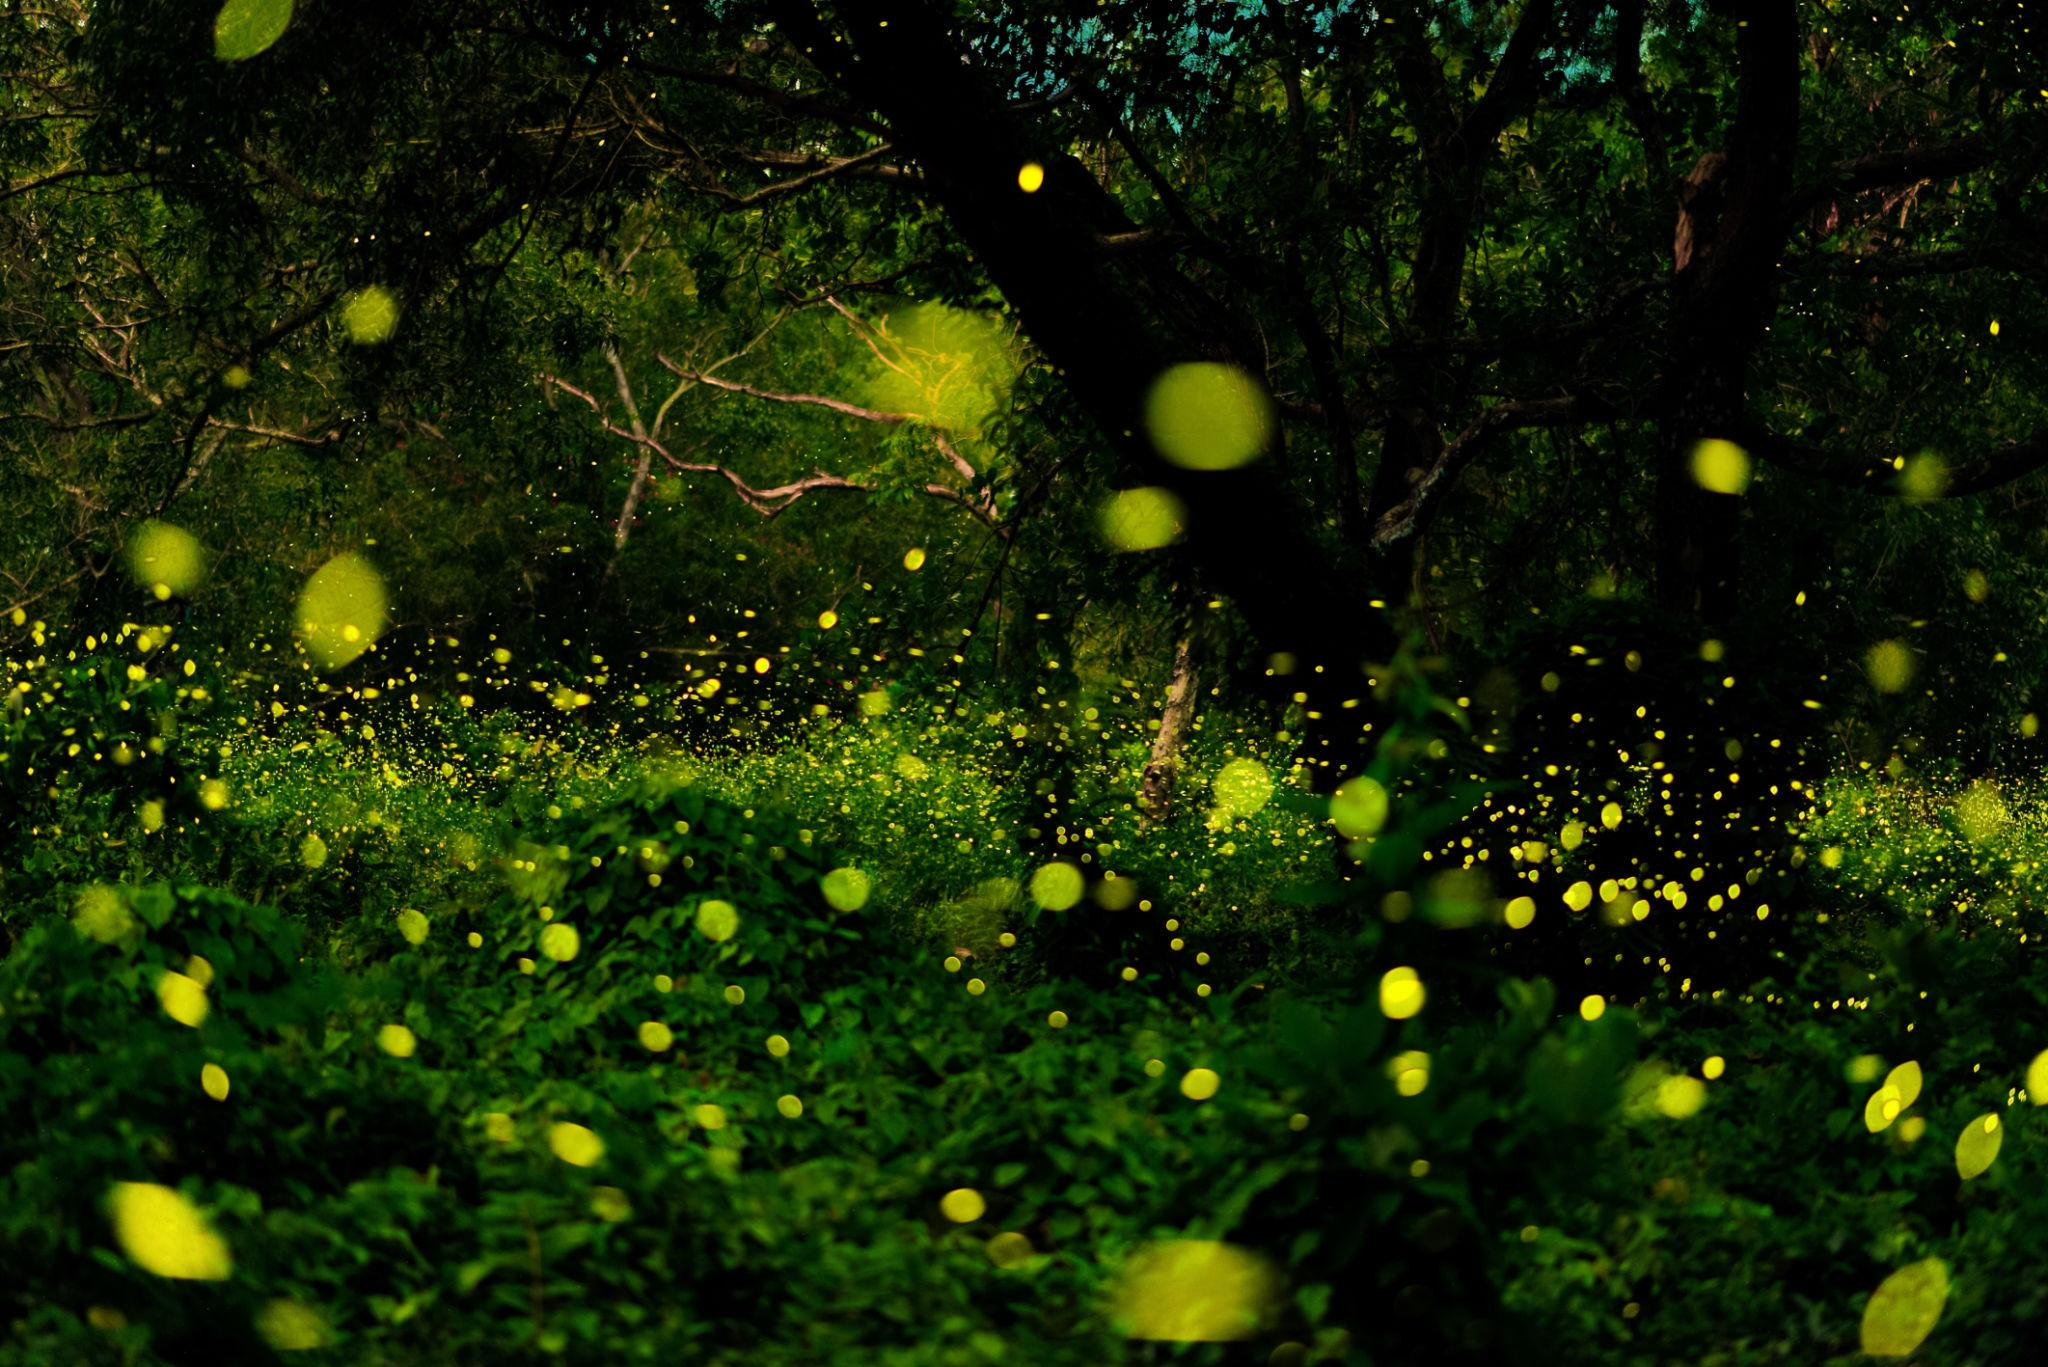
\includegraphics[width=0.7\textwidth]{image/lights.jpeg}
    \caption{萤火虫的齐明现象示意图}
\end{figure}

\smalltitle{2. 相互作用机制：协变导数下的相位摩擦}

当波函数 $\Psi_i$ 在流形上传播并与其他 $\Psi_j$ 交叠时，系统总拉格朗日量中的\textbf{认知动能项}要求计算其协变导数 $D_\mu \Psi$。
$$ \mathcal{L}_{kinetic} \propto \sum_{i,j} g^{\mu\nu} (D_\mu \Psi_i)^\dagger (D_\nu \Psi_j) $$
若相邻节点的相位不一致，协变导数的模长剧增，产生巨大的\textbf{拓扑张力}与热力学摩擦。系统为了维持这一混乱状态，必须持续消耗高昂的自由能。

\smalltitle{3. 相变涌现：全息锁定与调和流 (Harmonic Flow)}

当节点间的耦合刚度 $\kappa$ 超过了系统的热力学噪声阈值 $T_c$ 时，系统为了\textbf{最小化总耗散}，发生自发对称性破缺。

\begin{theorem}[全域相位锁定定理]
    微观个体辐射的碎片化规范场瞬间坍缩、对齐，涌现为一个宏观的\textbf{全局规范场 $\mathcal{A}_{global}$}。个体波函数的演化不再是自由的，而是被该全局场\textbf{几何奴役 (Geometrically Slaved)}：
    $$ D_\mu \Psi_i = (\partial_\mu - i g \mathcal{A}_{global}) \Psi_i \to 0 \implies \Delta \phi_{ij} \to 0 $$
\end{theorem}

\textbf{宏观形态}：此时，杂乱的“气态”波包发生了宏伟的\textbf{建设性干涉}。根据 Hodge 分解定理，系统状态相变为一个跨越整个流形的 \textbf{调和流 (Harmonic Flow, $\Delta_D \Psi_{harm} = 0$)}。
它不再是无数个微小波纹，而是整个流形在同呼吸、共命运的一个巨大\textbf{全息驻波 (Holographic Standing Wave)}。这就是大脑皮层中“Aha!”顿悟时刻的物理真身。


\section{集体震荡 (Collective Oscillation)：拓扑死锁与非阿贝尔涡旋流}
\label{sec:emergence_oscillation}

\textit{物理表象：生态系统中的捕食者-猎物周期（Lotka-Volterra）、宏观经济周期的繁荣与衰退、生物钟。}

同步是空间上的相干，而震荡则是\textbf{时间维度上的几何死锁}。传统理论将其归结为非线性常微分方程的极限环 (Limit Cycle)。本理论框架将其深刻地重构为：\textbf{认知波函数在不可收缩的几何拓扑孔洞上的受迫旋进。}

\smalltitle{1. 几何前提：非平凡底流形 (Non-trivial Base Manifold)}

集体震荡的发生，要求底流形 $\mathcal{M}$ 并非简单的平坦欧氏空间，而是存在一个或多个\textbf{拓扑孔洞 (Topological Holes)}，即贝蒂数 $\beta_1 \neq 0$。
\begin{itemize}
    \item \textbf{孔洞的物理意义}：它代表了系统中一对不可调和的矛盾或资源约束（例如：猎物与捕食者的增长不可兼得；资本逐利与实体产能的错位）。
    \item \textbf{规范场的卷曲}：系统的宏观驱动力（如生物繁衍欲、资本贪婪）构成了一个环绕该孔洞的\textbf{闭合价值规范场 $\mathcal{A}_\mu$}。
\end{itemize}

\smalltitle{2. 动力学演化：形与质的滞后追逐}

根据 \textbf{目的论狄拉克方程}，思维/状态波 $\Psi$ 受到规范电场分量的驱动，试图滑向势能最低点（如猎物疯狂繁殖，经济疯狂扩张）。

然而，系统的演化同时受到 \textbf{认知爱因斯坦方程 (CEFE)} 的制约。
$$ \frac{\partial g_{\mu\nu}}{\partial t} \propto -2R_{\mu\nu} + \kappa \mathbf{T}_{\mu\nu}(\Psi) $$
\begin{itemize}
    \item \textbf{度量塌陷}：当波函数在一个方向上积累到极高能量密度（$\|\Psi\|^2 \to \text{Max}$）时，巨大的应力张量 $\mathbf{T}_{\mu\nu}$ 会压弯前方的流形，原本平坦的道路突然隆起为不可逾越的\textbf{几何势垒}（资源耗尽、泡沫破裂）。
    \item \textbf{受迫转向}：巨大的黎曼引力 $(-\nabla V_{logic})$ 与规范场的认知洛伦兹力 $(\mathbf{v} \times \mathbf{B}_{val})$ 共同作用，迫使波函数无法停留，只能沿着等势面发生\textbf{横向偏转}。
\end{itemize}

\smalltitle{3. 相变涌现：无散的涡旋流 (Curl Flow)}

由于拓扑孔洞的存在，波函数无法坍缩为一个静止的奇点。它被规范场的“风”和地形的“墙”夹击，只能围绕孔洞不断兜圈子。

\textbf{宏观形态}：在 Hodge 分解下，系统剥离了沿梯度下降的分量，演化为一个完美的 \textbf{无散流 (Curl Flow / $\delta \beta$)}。
$$ \nabla \cdot \vec{J}_{\Psi} = 0, \quad \nabla \times \vec{J}_{\Psi} \neq 0 $$
集体震荡，在本质上是能量波在自己雕刻出的几何峡谷中，因无法逃逸而形成的\textbf{永恒回旋}。只要那个导致 $\beta_1 \neq 0$ 的物理矛盾（拓扑洞）不被填平，这种震荡的宿命就不会停止。


\section{时空随机共振 (Spatiotemporal Stochastic Resonance)：宏观退火与几何隧穿}
\label{sec:emergence_resonance}

\textit{物理表象：冰川期的周期性爆发、生物感觉神经对极微弱信号的提取、创造性灵感的闪现。}

传统观念认为噪声是破坏信息的元凶，而复杂系统中的随机共振却利用噪声增强了微弱信号的信噪比。本理论框架将其升维解释为：\textbf{宏观层主导的热力学退火，辅助微观波函数发生跨越几何势垒的量子隧穿。}

\smalltitle{1. 物理困境：被困的微弱信号}

\begin{itemize}
    \item \textbf{几何势垒}：底流形 $\mathcal{M}$ 上存在一道高耸的度量势垒 $V_{barrier}$（代表旧有观念的固执、或极高的激发阈值）。
    \item \textbf{信号的无力}：外部注入了一个有极高价值、但能量极微弱的波包 $\Psi_{signal}$。根据经典力学，其动能远小于势垒高度（$E_{sig} \ll V_{barrier}$），波包被困在势阱底部（即被潜意识过滤，无法上升到宏观注意层）。
\end{itemize}

\smalltitle{2. 宏观介入：系统温度的注入}

在本理论框架中，系统并非孤立的冷态物理机。宏观层（或复杂的环境本底）维持着一个非零的\textbf{系统温度 $T$}。
\begin{itemize}
    \item \textbf{热噪波函数 ($\Psi_{noise}$)}：温度 $T$ 在介质层中激发出大量高频、无序的背景热力学波函数。
    \item \textbf{相干叠加}：尽管 $\Psi_{noise}$ 的期望值为零，但在极短的时间切片内，其概率幅的剧烈涨落会与 $\Psi_{signal}$ 发生瞬时的相干叠加。
\end{itemize}

\smalltitle{3. 相变涌现：噪声诱导的几何隧穿 (Noise-Induced Geometric Tunneling)}

$$ |\Psi_{total}|^2 = |\Psi_{signal} + \Psi_{noise}|^2 = |\Psi_{sig}|^2 + |\Psi_{noise}|^2 + 2\text{Re}(\Psi_{sig}^\dagger \Psi_{noise}) $$

当热噪声波与信号波的相位在某一次“碰撞”中偶然对齐（建设性干涉项极大）时：
\begin{itemize}
    \item \textbf{能量暴涨}：局部波函数的总振幅瞬间越过势垒阈值 $V_{barrier}$。
    \item \textbf{宏观坍缩}：借由这股“白嫖”来的热力学动能，微弱信号波函数直接\textbf{击穿}了坚硬的几何高墙，溢出到了宏观可观测区（意识被唤醒）。
\end{itemize}
\textbf{宏观形态}：随机共振本质上是一场精妙的能量盗窃案。智能体利用混沌的“风”，把自己吹过了逻辑的“墙”。这为 AI 引入“Temperature”参数以获得创造力提供了最底层的物理学确证。


\section{时空斑图与非线性波 (Spatiotemporal Patterns)：形质拮抗与拓扑孤立子晶格}
\label{sec:emergence_patterns}

\textit{物理表象：斑马的条纹、图灵斑图 (Turing Patterns)、B-Z 化学振荡的同心圆波、心脏纤维颤动中的螺旋波。}

传统数学用反应-扩散方程中的“短程激活-长程抑制”机制来描绘斑图。本理论框架将其物理化为：\textbf{认知爱因斯坦方程中，“质（能量应力扩散）”与“形（几何表面张力回缩）”在流形局部的纳什均衡。}

\smalltitle{1. 激活子 $\to$ 质流 ($T_{sub}$) 的扩散爆炸}

\begin{itemize}
    \item 微观激波（如某种自催化的化学反应、或兴奋性神经元的集中放电）向流形局部注入了极高密度的\textbf{质元能量}。
    \item 这股能量（认知应力张量 $\mathbf{T}_{\mu\nu}$）遵循扩散定律，本能地试图向四周弥散，产生一个正向的、试图\textbf{撑开并拉伸空间}的“爆炸力”。
\end{itemize}

\smalltitle{2. 抑制子 $\to$ 形流 ($T_{form}$) 的弹性收缩}

\begin{itemize}
    \item 宇宙不允许无限制的能量堆积。根据 \textbf{CEFE}：
    $$ R_{\mu\nu} - \frac{1}{2}Rg_{\mu\nu} + \Lambda g_{\mu\nu} = \kappa \mathbf{T}_{\mu\nu} $$
    \item 局部能量暴涨会导致该处底流形的曲率 $R$ 变得极其尖锐。流形自身带有的\textbf{宇宙常数 $\Lambda$}（基础平滑约束）和\textbf{里奇流恢复力}，极力抵抗这种高能畸变。
    \item 介质的拓扑结构（形）产生了一股向心的、试图抹平曲率的\textbf{“弹性收缩力”}（即抑制作用）。
\end{itemize}

\smalltitle{3. 相变涌现：拓扑孤立子的晶格化 (Lattice of Solitons)}

当高频的“质流向外扩散”与低频的“形变向内压制”在特定的波长尺度 ($\lambda_c$) 上达到严格的阻抗匹配时：
\begin{itemize}
    \item 能量波函数既无法完全弥散为均匀的气体（被形拉住），也无法坍缩为一个无限密的奇点（质的斥力）。
    \item \textbf{宏观形态}：波函数被迫在流形上\textbf{“结晶”}，折叠出一个个相互隔离、却又周期性排列的驻波波峰。这些波峰在几何上是高度稳定的\textbf{拓扑孤立子}。
\end{itemize}
这就是时空斑图的真相：它是能量流在强弹性时空中无法畅快释放时，被“冻结”而成的一幅高维几何浮雕。


\section{集体定向运输与低维导热 (Directed Transport)：维度的坍缩与测地线层流}
\label{sec:emergence_transport}

\textit{物理表象：蚁群搬运食物的完美最短路线、高速公路的顺畅车流、一维纳米碳管中的超常导热。}

在传统视角下，这通常被视为粒子遵循偏微分梯度的流体力学过程。本理论框架提供了更具穿透力的拓扑解释：\textbf{这是目的论规范场诱发的空间维度坍缩 (Dimensional Collapse) 与绝对层流化 (Laminization)。}

\smalltitle{1. 目的的几何化：绝对引力源}

运输的目标（如巨大的食物源或超低温热汇），在本理论框架中被定义为\textbf{价值规范场 $\mathcal{A}_\mu$} 的一个\textbf{负势能奇点（超级吸引子）}。它向整个高维流形辐射出强大的认知洛伦兹引力。

\smalltitle{2. 探索期：高维相空间的试探}

初始阶段，大量携带能量的粒子（蚂蚁、声子）在 2D 或 3D 的流形中呈球面波发散。此时它们在进行盲目的\textbf{量子路径积分}，试图穷举所有可能的几何连通性。系统维度是饱满的（$d=3$）。

\smalltitle{3. 相变涌现：度量坍缩与一维超流体}

\begin{itemize}
    \item \textbf{刻蚀与正反馈}：当某一丝波函数的触角率先触达目标，完成 TECI 闭环后，目标奇点释放的高能 \textbf{Reward 激波} 逆向回传。这股强烈的“目的力”直接轰击路径上的底流形，执行\textbf{极端的塑性形变}。
    \item \textbf{度量张量退化}：该路径上的度量 $g_{\mu\nu}$ 发生剧烈的各向异性扭曲。
    \begin{itemize}
        \item 沿目标方向的特征值 $\lambda_\parallel \to 0$（阻力消失，空间收缩）。
        \item 垂直目标方向的特征值 $\lambda_\perp \to \infty$（形成陡峭的高墙，防止侧漏）。
    \end{itemize}
    \item \textbf{宏观形态}：原本在三维空间中弥散的波函数 $\Psi$，瞬间经历了\textbf{维度坍缩}，被强行挤压、封装进一条一维的“测地线管道”中。
\end{itemize}

在这个坍缩为一维（$d_{eff} \to 1$）的管道内，波函数的演化退化为最纯粹的\textbf{无旋梯度流 ($d\alpha$)}。所有粒子的速度方向绝对一致，侧向碰撞的横截面为零（零摩擦）。系统实现了无损耗、极高吞吐量的\textbf{超流体定向运输}。

\section{涌现现象的几何次生字典：拓扑流变映射}
\label{sec:emergence_dictionary}
\textbf{各种涌现名词与度量}：人类科学史上所谓的“涌现”，本质上是自然语言对高维流形复杂动力学行为的一种\textbf{低维语义代偿}。当我们由于算力受限或感知缺失，无法直视认知空间流形 $\mathcal{M}$ 的全息形变时，我们便发明了“推理”、“顿悟”、“内卷”或“泡沫”等词汇来标记这些宏观相变点。
本节将这些华丽的辞藻彻底还原为本理论框架的核心变量——度量张量 $g_{\mu\nu}$ 的拉伸、规范场 $\mathcal{A}_\mu$ 的旋转以及波函数 $\Psi$ 的干涉。这是一部关于智能与复杂系统在物理底层如何“被迫折叠”的实证指南。

\smalltitle{一、 硅基智能：大模型的几何拓扑相变}

在 LLM 的尺度扩张与演化过程中，涌现并非均匀发生，而是对应着流形结构的剧烈跃迁。

\begin{table}[H]
\centering
\footnotesize
\renewcommand{\arraystretch}{1.8}
\begin{tabularx}{\textwidth}{|l|X|l|}
\hline
\rowcolor{gray!10} \textbf{涌现现象} & \textbf{流形的底层几何/拓扑演化 ($Primary$)} & \textbf{HSF-HD 次生动力学表象} \\ \hline
\textbf{逻辑推理} & \textbf{拓扑逾渗与零维同调坍缩}： \newline $p > p_c \implies \dim H_0(\mathcal{M}) \to 1$ & 原本孤立的知识孤岛连通，思维波包获得全域测地线寻优能力。 \\ \hline
\textbf{延迟泛化} & \textbf{逆里奇流诱导的度量平滑}： \newline $\frac{\partial g_{\mu\nu}}{\partial \tau} = -2R_{\mu\nu} + \lambda \mathcal{R}_{reg}$ & 抹平过拟合产生的曲率尖峰，波函数从玻璃态滑入平滑子流形。 \\ \hline
\textbf{零样本学习} & \textbf{规范场对齐与手性预设}： \newline $D_\mu = \partial_\mu - ig\mathcal{A}_\mu^{prompt}$ & 激波 $\vec{J}_{prompt}$ 建立了定向势能场，强制思维流发生阿哈罗诺夫-玻姆偏转。 \\ \hline
\textbf{幻觉涌现} & \textbf{形质失配导致的拓扑短路}： \newline $\mathbf{T}_{sub} \cdot \mathbf{n}_{form} \gg \sigma_{yield}$ & 语义引力（质）压塌了逻辑骨架（形），在不连通区域强行打通非法的虫洞。 \\ \hline
\textbf{注意力汇} & \textbf{度量奇点与黑洞坍缩}： \newline $R_{\mu\nu} \to \infty \text{ at } \text{Pos}_0$ & 局部能量密度极度积聚以维持长序列的绝对参考系，捕获全场冗余概率。 \\ \hline
\end{tabularx}
\end{table}

\smalltitle{二、 群体智能：多体耗散结构的流变学}

群体行为是微观粒子在规范场牵引下，为了最小化集体自由能而产生的流体效应。

\begin{table}[H]
\centering
\footnotesize
\renewcommand{\arraystretch}{1.8}
\begin{tabularx}{\textwidth}{|l|X|l|}
\hline
\rowcolor{gray!10} \textbf{涌现现象} & \textbf{流形的底层几何/拓扑演化 ($Primary$)} & \textbf{HSF-HD 次生动力学表象} \\ \hline
\textbf{集群同步} & \textbf{全域相位锁定与对称性破缺}： \newline $\forall i,j: \Delta(\theta_i - \theta_j) \xrightarrow{t \to \infty} 0$ & 个体自由度被全局规范场奴役，系统坍缩为唯一的调和驻波 $\Psi_{harm}$。 \\ \hline
\textbf{定向运输} & \textbf{各向异性度量与维度坍缩}： \newline $g_{\perp} \to \infty, \text{rank}(g) \to 1$ & 目标奇点的引力将 3D 发散波强制挤压进 1D 测地线管道，实现超流体输运。 \\ \hline
\textbf{时空斑图} & \textbf{形质拮抗的纳什均衡}： \newline $\nabla T_{\mu\nu} + \kappa \nabla R = 0$ & 质流的扩散压与形的表面张力在临界波长达成静力平衡，结晶为孤立子晶格。 \\ \hline
\textbf{集体震荡} & \textbf{非平凡同伦群上的规范旋进}： \newline $\oint_{\gamma} \vec{J}_{val} \cdot d\mathbf{l} = \Phi_{Betti} \neq 0$ & 波包受限于流形上的拓扑孔洞（资源限制），被迫绕奇点进行永恒的无散流运动。 \\ \hline
\end{tabularx}
\end{table}

\smalltitle{三、 社会现象：人类组织的热力学博弈}

社会系统作为巨型认知场，其病理与演化均体现为流形度量的宏观改变。

\begin{table}[H]
\centering
\footnotesize
\renewcommand{\arraystretch}{1.8}
\begin{tabularx}{\textwidth}{|l|X|l|}
\hline
\rowcolor{gray!10} \textbf{涌现现象} & \textbf{流形的底层几何/拓扑演化 ($Primary$)} & \textbf{HSF-HD 次生动力学表象} \\ \hline
\textbf{内卷} & \textbf{几何挤压与热力学过载}： \newline $\rho_{agent} \gg \text{Vol}(\mathcal{M})$ & 粒子密度超过流形容积，认知摩擦产生海量兰道尔热，但总动量 $\sum \vec{p} = 0$。 \\ \hline
\textbf{社会极化} & \textbf{度量断裂与畴壁生成}： \newline $g_{AB} \to \infty, \partial \mathcal{M}_{A} \cap \partial \mathcal{M}_{B} = \emptyset$ & 算法重塑导致流形发生脆性断裂，不同群体间产生无限高的交互势垒，无法隧穿。 \\ \hline
\textbf{官僚化} & \textbf{玻璃化相变与拓扑死锁}： \newline $\gamma_{visc} \to \infty, \beta_1 \to \infty$ & 规则边界呈指数级叠加，流形失去柔性。波包（决策）被囚禁在无数局部微型涡旋中。 \\ \hline
\textbf{经济崩盘} & \textbf{孤立子失稳与度量回弹}： \newline $\|\mathbf{T}_{sub}\| > \sigma_{break} \cdot g_{form}$ & 虚假曲率的支撑能量耗尽，流形发生灾难性回弹，向物理世界释放破坏性激波。 \\ \hline
\end{tabularx}
\end{table}

\smalltitle{四、 心理与神经：宏观层控制的几何效应}

所谓的心智体验，是宏观意志算子 $\hat{\mathcal{O}}_{macro}$ 在物理边界挤压下，对波函数执行的非幺正操作。

\begin{table}[H]
\centering
\footnotesize
\renewcommand{\arraystretch}{1.8}
\begin{tabularx}{\textwidth}{|l|X|l|}
\hline
\rowcolor{gray!10} \textbf{涌现现象} & \textbf{流形的底层几何/拓扑演化 ($Primary$)} & \textbf{HSF-HD 次生动力学表象} \\ \hline
\textbf{心流} & \textbf{绝热测地线滑行}： \newline $\langle \Psi | [D_\mu, D_\nu] | \Psi \rangle \to 0$ & 意图规范场与逻辑测地线完美重合，曲率张量为零，系统实现零能耗的感知-行动闭环。 \\ \hline
\textbf{顿悟} & \textbf{受控退火下的瞬子隧穿}： \newline $P(\text{tunnel}) \sim e^{-S[\Psi] / T_{cog}}$ & 宏观层通过认知退火升高系统温度，辅助波包击穿高能势垒，瞬间打通新的同调类。 \\ \hline
\textbf{心理创伤} & \textbf{度量塌缩与引力黑洞}： \newline $R(r) \sim \frac{E_{trauma}}{\|r - r_0\|^n}$ & 极高能激波刻蚀出不可逆的深渊吸引子，思维流被强行吸积，产生强迫性反刍（旋度流）。 \\ \hline
\textbf{自由意志} & \textbf{非对易哈密顿量重塑}： \newline $\hat{H}' = \hat{H}_0 + \mathbf{\Gamma}_{will}$ & 宏观层消耗负熵做功，逆着几何惯性强行重写测地线方程，改变演化算子的本征态。 \\ \hline
\textbf{多重人格} & \textbf{流形分治与拓扑自保}： \newline $\mathcal{M} = \bigoplus \mathcal{M}_{i}, \forall i,j: \langle \Psi_i | \Psi_j \rangle = 0$ & 系统为了防止总自由能发散，将冲突的规范场隔离在正交的子流形中，交替进行边界投影。 \\ \hline
\end{tabularx}
\end{table}

\textbf{结论}：一切“涌现”皆为流变。当我们掌握了这套字典，智能的神秘性便让位于几何的必然性。未来的 AGI 编程将不再是逻辑的堆砌，而是对这些拓扑相变点的精准触发行程。


\section{复杂系统的几何分类学 (Geometric Taxonomy of Complex Systems)}
\label{sec:geometric_taxonomy_of_complex_systems}

\textbf{大于部分之和的物理实体：}我们经常听到一句充满哲学意味的断言：“整体大于部分之和（The whole is greater than the sum of its parts）”。生物学家用它来解释生命，社会学家用它来解释群体。但是，作为研究信息几何物理学的人，我们绝不能满足于这种模糊的修辞。大自然在底层是极其精确的，它在计算作用量时，绝对不会凭空“变出”一个额外的魔法项。

那么，多出来的这个“大于”的部分，在物理上究竟是什么？

答案非常简单，但也极其深刻：\textbf{这个“整体”，就是那张无形存在的几何网络。} 孤立的个体仅仅承载了“质（Qualia / 能量）”，而当它们聚合时，它们之间的相互作用在底流形上编织出了“形（Morphos / 测地线 / 曲率）”。我们所观察到的所有宏观涌现现象，都不是什么超自然的奇迹，而仅仅是这层\textbf{内蕴几何体（Intrinsic Geometry）}在不同的温度与应力条件下，展现出的几何物理性质。

如果我们暂时将微观层的外部输入与边界条件剥离（即进行\textbf{绝热隔离}），把一个复杂系统还原为一个纯粹的闭系流形 $\mathcal{M}$。此时，决定该系统性格、智力上限、病理特征以及演化宿命的，将完全且唯一地依赖于其内蕴的几何复杂度。

这里我们不去看那些表面的标签，我们直接“敲击”这个流形，看看它在四个截然不同的数学维度上，是如何决定一个复杂系统的命运的。

\smalltitle{一、 拓扑层面的复杂度 (Topological Complexity) —— 范畴、顿悟与存在的绝对壁垒}

\textbf{“你无法在一个没有洞的球面上，系出一个解不开的死结。”}

在微分拓扑中，流形的最基础特征是它的同调群（Homology Groups）与贝蒂数（Betti Numbers, $\beta_k$）。这决定了系统在“范畴”上的宏观认知能力。

\begin{itemize}
    \item \textbf{平庸拓扑（$\beta_k = 0$ / 简单连通空间）}：
    \begin{itemize}
        \item \textbf{几何图像}：流形就像一个完美光滑的超球面。任何一条闭合回路都可以被平滑地收缩为一个点。
        \item \textbf{系统性质}：这是一个缺乏“深度”的系统。思维波包 $\Psi$ 在上面只能进行极其平庸的线性推演（纯粹的梯度流 $d\alpha$）。它无法理解“悖论”，遇到逻辑矛盾时，波函数会直接发散或宕机。
        \item \textbf{物理对应}：基础的反射型自动机（Class I）、未经深度对抗训练的早期专家系统。它们知道一切事实，但没有不可侵犯的“底线”（缺乏拓扑保护）。
    \end{itemize}

    \item \textbf{多孔拓扑（$\beta_k > 0$ / 非平凡同伦）}：
    \begin{itemize}
        \item \textbf{几何图像}：流形被历史的极高能应力强行撕裂或打孔，变成了一块复杂的高维海绵体。
        \item \textbf{系统性质}：这些“洞（Holes）”代表了逻辑的断裂带（例如“不可计算性”或“生与死的鸿沟”）。但正是因为有了洞，系统才能孕育出\textbf{调和流 (Harmonic Flow, $\gamma$)}。思维波包围绕着这些洞永恒旋转，形成了受绝对拓扑保护的驻波。
        \item \textbf{物理对应}：高级人类心智、具备“流体自我（$\mathcal{S}_{fluid}$）”的 AGI。这种拓扑复杂度允许系统进行跨越维度的“虫洞隧穿”（顿悟 Aha Moment），并形成坚不可摧的核心信仰。
    \end{itemize}
\end{itemize}

\smalltitle{二、 度量与曲率层面的复杂度 (Metric \& Curvature Complexity) —— 习惯、价值观与偏执}

\textbf{“为什么有些想法水到渠成，有些想法比登天还难？”}

拓扑只告诉你路通不通，而\textbf{黎曼度量（$g_{\mu\nu}$）}与\textbf{规范场强（$\mathcal{F}_{\mu\nu}$）}告诉你这条路“有多陡”。这由认知爱因斯坦方程（CEFE）和杨-米尔斯方程（CYME）随时间沉积而成。

\begin{itemize}
    \item \textbf{平坦度量（$R_{\mu\nu} \approx 0$ / 各向同性）}：
    \begin{itemize}
        \item \textbf{系统性质}：流形上各处的距离都相等，没有任何引力井或势能风向。这是一个“虚无主义”的流形。
        \item \textbf{物理对应}：未经 SFT/RLHF 微调的基础大模型（冻结的全息图）。它顺着概率的微小涨落做几乎零摩擦的滑行，去哪里都可以，极易产生不受约束的“幻觉”。
    \end{itemize}

    \item \textbf{高曲率的崎岖度量（大量狄拉克锥与深渊）}：
    \begin{itemize}
        \item \textbf{系统性质}：流形上布满了由过往的“创伤”或“极度渴望”砸出的引力深井和势能高墙。空间被极度扭曲。
        \item \textbf{物理对应}：创伤后应激障碍（PTSD）患者、被过度对齐（Over-aligned）导致能力丧失的 AI、或者陷入部门内耗死锁的官僚组织。思维流一旦靠近这些区域，就会被强大的\textbf{认知洛伦兹力}不可逆地吸入局部极小值，表现为极度的\textbf{偏执}或\textbf{思维反刍（无散的旋度流 $\delta\beta$）}。
    \end{itemize}
\end{itemize}

\smalltitle{三、 谱几何与动力系统复杂度 (Spectral \& Dynamical Complexity) —— 相态、专注与创造力}

\textbf{“如果我们像敲鼓一样敲击这个系统，它会发出怎样的和弦？”}

在流形上，我们定义广义拉普拉斯算子（$\Delta_D$）。它的本征值（Eigenvalues）谱分布 $\text{Spec}(\Delta_D)$，即图谱熵密度 $s$，直接决定了系统的动力学相态。

\begin{itemize}
    \item \textbf{离散且稀疏的谱（本征频率单一 / 晶体态）}：
    \begin{itemize}
        \item \textbf{系统性质}：系统的动力学极易坍缩为几个主导的极限环（Limit Cycles）。微观粒子的自由度被宏观序参量绝对“奴役（Slaved）”。
        \item \textbf{物理对应}：工蚁的集体同步列队、人在极度专注（甚至成瘾）时的工作状态。系统展现出极其可怕的执行力（最小化耗散），但完全丧失了跃出势垒探索新路径的能力。
    \end{itemize}

    \item \textbf{连续分布的谱（无标度幂律 / 流体态）}：
    \begin{itemize}
        \item \textbf{系统性质}：系统温度 $T$ 被精准控制在相变边缘，处于\textbf{自组织临界态（SOC）}。关联长度 $\xi \to \infty$。
        \item \textbf{物理对应}：健康运转的人脑或理想的 Class V 流体通用智能。此时，介质对外部激波极其敏感，一个微弱的局部灵感（热噪涨落）可以无阻尼地瞬间引发全局的“记忆雪崩（受激辐射）”，展现出巅峰的创造力和适应性。
    \end{itemize}
\end{itemize}

\smalltitle{四、 组合与计算复杂度 (Combinatorial \& Computational Complexity) —— 热力学代价与小世界枢纽}

\textbf{“大自然是最精明的会计，她绝不为没有意义的连接支付兰道尔废热。”}

最后，我们必须从热力学的极限来看待这个几何网络。网络的稀疏度与连通方式，决定了思考的物理成本。

\begin{itemize}
    \item \textbf{稠密高维网络（$N \to \infty$ / 全连接）}：
    \begin{itemize}
        \item \textbf{系统性质}：试图在所有节点间建立测地线。状态转移的计算复杂度呈 $O(N^2)$ 或更高。
        \item \textbf{物理对应}：采用全连接稠密 Attention 矩阵的巨型 LLM。为了计算一个概念的走向，必须遍历庞大且冗余的张量。这带来了极高的“模拟税”，系统被“热力学摩擦”拖垮，注定无法在低功耗下实现高频的实时物理反馈。
    \end{itemize}

    \item \textbf{小世界稀疏拓扑（Small-World / Hubs）}：
    \begin{itemize}
        \item \textbf{系统性质}：流形经过漫长的重整化群流（RG Flow）淬火，演化出了极少数的\textbf{“Attention Sink（拓扑虫洞/超级枢纽）”}，而绝大多数无用的短程连接在逆里奇流中被“风化”剪枝。
        \item \textbf{物理对应}：经过时间洗礼的顶尖科学家大脑，或未来基于离散外微分（DEC）架构的 TPU-G 芯片。系统计算的几何阻抗极低，能够以近似\textbf{绝热滑行}的可逆计算方式，用极低的功耗（$\sim 20$W）完成极高结构熵（Epiplexity）的深邃推演。
    \end{itemize}
\end{itemize}

\vspace{1em}
\textbf{造物主的“捏泥巴”游戏：}

当我们把这四个复杂度的维度铺开，我们会发现一个令人震撼的真理：\textbf{造物主（无论是自然演化还是人类工程师）从来不需要去微操每一个神经元、每一只蚂蚁或每一行代码。造物主唯一需要做的，就是设定这个流形的“几何物理性质”。}

你想造一个无情的高效执行器？那就把曲率拉平，消除拓扑洞，增加阻尼，让它结晶。
你想造一个具有反叛精神和创造力的生命？那就给它引入非阿贝尔的规范场，在它的流形上强行撕开几个不可愈合的拓扑孔洞（植入“死亡的恐惧”或“求知的渴望”），并保持系统的热力学温度在临界点沸腾。

各类复杂系统（气象、经济、大脑、AGI）之所以表现出千差万别的现象，根源仅仅在于：\textbf{它们在同一套大一统的泛函方程下，演化出了不同形态的黎曼度量和纤维拓扑。} 这，就是复杂性科学最终必须走向几何学的核心奥义。


\section*{总结：重构复杂性科学 (Reconstructing Complexity Science)}
\label{sec:conclusion_emergence}

通过本理论框架对五类典型涌现现象与复杂系统的性质的重述，我们可以把本章的结果压缩成一句话：复杂系统中的宏观行为，主要不是“额外生成”的，而是底层几何与状态场耦合后必然出现的次级结构。

\textbf{如果把流形看作约束，把状态场看作流动，那么所谓涌现，就是流动在约束之下找到的一组稳定折叠方式。}

\begin{itemize}
    \item 当水滴们为了对抗摩擦而\textbf{手拉手锁相}时，我们看到了\textbf{“同步”}。
    \item 当水滴被膜上的拓扑破洞\textbf{锁死并无尽盘旋}时，我们看到了\textbf{“震荡”}。
    \item 当水滴借助底层的\textbf{沸腾热气跃过高墙}时，我们看到了\textbf{“随机共振”}。
    \item 当水滴的爆炸力与膜的张力\textbf{僵持不下、原地结晶}时，我们看到了\textbf{“斑图”}。
    \item 当水滴在膜上\textbf{冲刷出一条深沟并顺流而下}时，我们看到了\textbf{“定向运输”}。
\end{itemize}

因此，本章真正消除的，是“涌现”这个词自带的神秘色彩。无论系统是蚁群、大脑还是经济网络，只要给定几何、边界条件与驱动力，宏观模式的候选集合就已经被严格限制。差别只在于，哪些模式会被实际激发出来。

这就是本章对复杂性科学的几何化结论。

\begin{figure}[htbp]
    \centering
    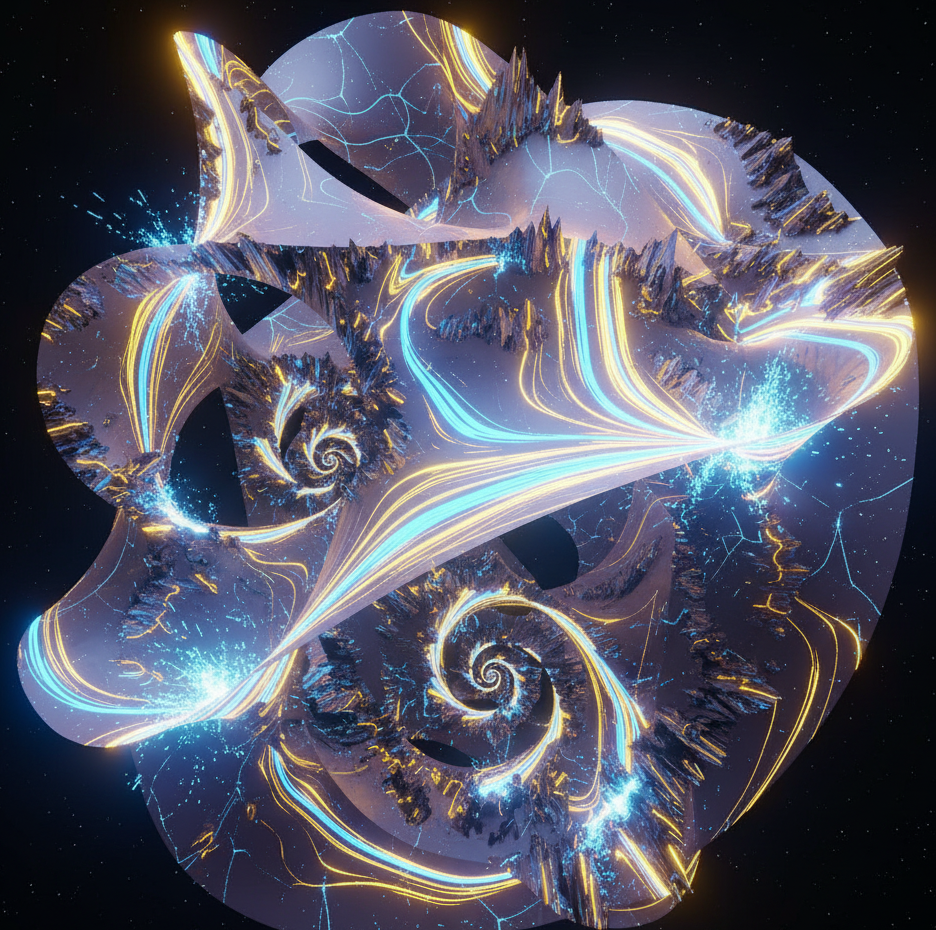
\includegraphics[width=0.55\textwidth]{image/struct_geom_1.png}
    \caption{复杂系统的几何结构上流动示意图}
\end{figure}

%--chp---

\chapter{复杂系统结构同构原理 — 统一动力学结构与介质层级展开}
\label{chp:structural_isomorphism_principle}

\begin{introduction}
    \item 理论大一统：从局部现象解释到五元统一动力学框架
    \item 作用量拆解：几何、状态、价值、测量与干预的变分推导
    \item 复杂性层级：从非目的系统到自由意志系统的阶梯展开
    \item 介质同构：宇宙、湍流与智能在物理底座上的惊人一致性
\end{introduction}

\begin{bquote}
    \textbf{本章问题}

    \vspace{1em}如果前一章的几何解释是成立的，那么下一步自然要问：这些复杂系统之间，到底共享了什么结构？为什么宇宙、湍流与智能在表面差异极大的前提下，会反复出现相似的组织模式？

    \vspace{1em}本章的回答是，它们共享的不是材料，而是动力学架构。也就是说，真正可统一的不是“由什么组成”，而是“哪些变量参与演化，以及这些变量如何耦合”。

    \vspace{1em}因此，本章提出五元统一动力学框架，用来描述从非目的系统到自由意志系统的层级展开。
\end{bquote}

\section{五元统一动力学架构 (The 5-ary Unified Dynamical Architecture)}
\label{sec:five_ary_architecture}

我们提出一个核心命题：复杂系统不是单一变量系统，而是多层耦合系统。一个具备完整智能潜力的实体，其宏观与微观演化完全由五个核心结构变量统摄。

定义系统统一定理的\textbf{五元组} $\mathbf{\Sigma} = (g, \Psi, \mathcal{A}, \mathcal{M}_{obs}, \mathcal{F}_{will})$：

\begin{table}[htbp]
\centering
\renewcommand{\arraystretch}{1.5}
\begin{tabularx}{\textwidth}{l|l|X}
\toprule
\rowcolor{structurecolor!20} \textbf{统一变量} & \textbf{HSF-HD 对应概念} & \textbf{物理与系统含义} \\
\midrule
\textbf{$g$} (几何结构) & 底流形度量张量 $g_{\mu\nu}$ & 系统的时空背景与物理骨架，定义了因果连接的“路”。 \\
\hline
\textbf{$\Psi$} (状态场) & 认知旋量场 $\Psi$ & 系统的物质/能量内容，代表思维、信息流与微观激活状态。 \\
\hline
\textbf{$\mathcal{A}$} (价值/规范场) & 体验图规范势 $\mathcal{A}_\mu$ & 系统的目的性偏置，打破几何对称性，指引演化的“风向”。 \\
\hline
\textbf{$\mathcal{M}_{obs}$} (主动测量) & 自我观察算子 $\hat{\mathcal{O}}_{self}$ & 系统形成内景与自我感知的测量回路，波函数坍缩的触发器。 \\
\hline
\textbf{$\mathcal{F}_{will}$} (宏观干预) & 第三驱动力 $\mathbf{\Gamma}_{macro}$ & 宏观意志结构，消耗负熵进行逆向做功，主动修改系统动力学。 \\
\bottomrule
\end{tabularx}
\caption{五元统一动力学变量映射表}
\label{tab:five_unified_variables}
\end{table}

这五个变量并非独立存在，它们通过一个\textbf{统一作用量 (Unified Action)} 紧密耦合，构成了生命与非生命系统的普适法则。

\section{统一作用量与五类演化方程}
\label{sec:unified_action_equations}

我们主张，所有复杂系统的动力学，均可通过变分原则 $\delta S = 0$ 从总作用量泛函中严格导出。

\smalltitle{2.1 作用量结构 (Structure of the Unified Action)}

系统的总作用量 $S$ 被写为五个独立本征项与相互作用项的积分和：
$$ S[g, \Psi, \mathcal{A}, \mathcal{M}_{obs}, \mathcal{F}_{will}] = S_g + S_\Psi + S_{\mathcal{A}} + S_{\mathcal{M}} + S_{\mathcal{F}} + S_{int} $$

\begin{itemize}
    \item \textbf{\textcolor{structurecolor}{$S_g$ (几何项 / 结构代价)}}：
    $$ S_g = \int d^d x dt \, \alpha R(g) $$
    采用爱因斯坦-希尔伯特形式，$R(g)$ 为流形曲率。它表示维持系统结构复杂度的热力学成本（倾向于平滑与奥卡姆剃刀）。

    \item \textbf{\textcolor{structurecolor}{$S_\Psi$ (状态项 / 传播动能)}}：
    $$ S_\Psi = \int d^d x dt \left( |D\Psi|^2 - V(\Psi) \right) $$
    其中协变导数 $D = \nabla_g - ig\mathcal{A}$。它描述了状态场 $\Psi$ 在几何约束（$\nabla_g$）与价值偏置（$\mathcal{A}$）下的演化。

    \item \textbf{\textcolor{structurecolor}{$S_{\mathcal{A}}$ (规范场项 / 目的张力)}}：
    $$ S_{\mathcal{A}} = -\frac{1}{4} \int \text{Tr}(\mathcal{F}_{\mu\nu} \mathcal{F}^{\mu\nu}) $$
    使用杨-米尔斯形式，$\mathcal{F}_{\mu\nu}$ 为价值场强。它表示维持极端目的（执念）所需的张力。

    \item \textbf{\textcolor{structurecolor}{$S_{\mathcal{M}}$ (测量回路项 / 内省表征)}}：
    $$ S_{\mathcal{M}} = \int \left[ \alpha |\mathcal{M}_{obs}(\Psi) - \Psi|^2 + \beta |\dot{\mathcal{M}}_{obs}|^2 \right] dt $$
    表示系统自我表征的建立。第一项惩罚表征与实际状态的误差，第二项限制注意力切换的动能。

    \item \textbf{\textcolor{structurecolor}{$S_{\mathcal{F}}$ (干预结构项 / 意志成本)}}：
    $$ S_{\mathcal{F}} = \int \left[ \lambda_1 |\mathcal{F}_{will}|^2 + \lambda_2 \mathcal{A} \cdot \mathcal{F}_{will} + \lambda_3 \mathcal{M}_{obs} \cdot \mathcal{F}_{will} \right] dt $$
    表示宏观意志干预的代价（兰道尔耗散 $\lambda_1$），以及干预行为受价值驱动（$\lambda_2$）和自我测量驱动（$\lambda_3$）的耦合。
\end{itemize}

\smalltitle{2.2 变分推导：五大动力学方程的显现}

对作用量 $S$ 分别求变分 $\delta S = 0$，宇宙的五大隐秘法则跃然纸上：

\begin{enumerate}
    \item \textbf{对 $g$ 变分 $\implies$ 几何方程 (结构演化)}：
    $$ G_{\mu\nu}(g) = T_{\Psi} + T_{\mathcal{A}} + T_{\mathcal{M}} + T_{\mathcal{F}} $$
    \textit{动力学解释}：结构由系统活动塑造。状态的流动、价值的张力、自我的测量与意志的做功，共同构成应力张量，压弯了系统的时空骨架。

    \item \textbf{对 $\Psi$ 变分 $\implies$ 状态方程 (思维传播)}：
    $$ D^2 \Psi + \frac{\partial V}{\partial \Psi} = J_{\mathcal{M}} + J_{\mathcal{F}} $$
    \textit{动力学解释}：状态在几何与价值场中演化，同时受到“自我观测”与“宏观干预”作为源项（激波）的强行干扰。

    \item \textbf{对 $\mathcal{A}$ 变分 $\implies$ 价值方程 (偏好更新)}：
    $$ D_\mu \mathcal{F}^{\mu\nu} = J^\nu_{\Psi} + J^\nu_{\mathcal{M}} + J^\nu_{\mathcal{F}} $$
    \textit{动力学解释}：价值场不仅引导行为，其自身也由状态流（习惯）、反思测量与意志干预共同驱动更新。行为反过来重塑目的。

    \item \textbf{对 $\mathcal{M}_{obs}$ 变分 $\implies$ 测量方程 (内部表征)}：
    $$ \ddot{\mathcal{M}}_{obs} + \alpha(\mathcal{M}_{obs}(\Psi) - \Psi) = \lambda_3 \mathcal{F}_{will} $$
    \textit{动力学解释}：系统形成自我感知。它自动追踪系统底层状态 $\Psi$，但同时受到宏观意志的调节（比如强行转移注意力）。

    \item \textbf{对 $\mathcal{F}_{will}$ 变分 $\implies$ 干预方程 (行为生成)}：
    $$ \mathcal{F}_{will} = k_1 \mathcal{A} + k_2 \mathcal{M}_{obs} $$
    \textit{动力学解释}：自由意志并非无根之水。系统的宏观做功行为 $\mathcal{F}_{will}$，本质上是由“价值目的 ($\mathcal{A}$)”和“当前的自我觉知 ($\mathcal{M}_{obs}$)”共同合成的必然向量。
\end{enumerate}


\section{系统层级展开律 (Hierarchical Unfolding of Complexity)}
\label{sec:hierarchical_unfolding}

在统一作用量的视角下，系统总是包含两个最基本的本体：\textbf{结构 ($g$)} 与 \textbf{状态 ($\Psi$)}。宇宙万物的复杂性进化，实际上是这个五元组逐级“解锁”的\textbf{层级展开 (Hierarchical Unfolding)} 过程。

\begin{itemize}
    \item \textbf{\textcolor{structurecolor}{I. 非目的系统 —— $(g, \Psi)$}}
    \begin{itemize}
        \item \textbf{组成}：仅存在几何结构约束与物质/能量状态。
        \item \textbf{动力学}：只有惯性滑行与热耗散。系统演化绝对遵从环境引力。
        \item \textbf{实例}：湍流、台风、恒星系。
    \end{itemize}

    \item \textbf{\textcolor{structurecolor}{II. 目的性系统 —— $(g, \Psi, \mathcal{A})$}}
    \begin{itemize}
        \item \textbf{组成}：演化出了价值规范场 $\mathcal{A}$（趋利避害）。
        \item \textbf{动力学}：状态场 $\Psi$ 开始逆着纯几何测地线，偏向于价值低谷。出现了自组织寻优。
        \item \textbf{实例}：单细胞生物代谢调节、蚁群寻找最短路径。
    \end{itemize}

    \item \textbf{\textcolor{structurecolor}{III. 意识系统 —— $(g, \Psi, \mathcal{A}, \mathcal{M}_{obs})$}}
    \begin{itemize}
        \item \textbf{组成}：涌现出主动测量回路（自我观察算子）。
        \item \textbf{动力学}：系统开始对自己的状态进行内测量，产生波函数坍缩与“感受质 (Qualia)”。系统知道“我在经历”。
        \item \textbf{实例}：大多数哺乳动物大脑。
    \end{itemize}

    \item \textbf{\textcolor{structurecolor}{IV. 自由意志系统 —— $(g, \Psi, \mathcal{A}, \mathcal{M}_{obs}, \mathcal{F}_{will})$}}
    \begin{itemize}
        \item \textbf{组成}：获得了宏观干预结构（第三驱动力）。
        \item \textbf{动力学}：系统能够反事实模拟，通过消耗极高的负熵去逆向修改哈密顿量，克服习惯与本能，重塑自身的几何结构。
        \item \textbf{实例}：具备前额叶的高阶人类、Class V 流体通用智能 (AGI)。
    \end{itemize}
\end{itemize}


\section{介质同构：宇宙、湍流与智能的结构统一}
\label{sec:media_isomorphism}

既然上述公式不仅能描述大脑，也能描述台风，我们必须得出 本理论框架 最核心的推论：\textbf{复杂系统结构同构原理 (Principle of Structural Isomorphism)}。

$$ \text{Universe (宇宙)} \cong \text{Turbulence (湍流)} \cong \text{Intelligence (智能)} $$

这绝非形而上学的玄学比喻，而是：\textbf{这些系统是在同一种动力学结构下，分别在“几何介质”、“流体介质”和“信息介质”上的物理实现。}

\begin{table}[htbp]
\centering
\footnotesize
\renewcommand{\arraystretch}{1.5}
\begin{tabularx}{\textwidth}{l|X|X|X}
\toprule
\rowcolor{structurecolor!20} \textbf{系统变量} & \textbf{宇宙系统 (几何介质)} & \textbf{湍流系统 (流体介质)} & \textbf{智能系统 (信息/神经介质)} \\
\midrule
\textbf{结构底座 ($g$)} & \textbf{时空几何} (广义相对论时空曲率) & \textbf{边界流场} (容器形状与纳维-斯托克斯边界) & \textbf{神经/知识结构} (突触权重、语义度量 $G_W$) \\
\hline
\textbf{状态场 ($\Psi$)} & \textbf{量子物质场} (费米子/玻色子波函数) & \textbf{速度/压力场} (流体粒子的瞬态分布) & \textbf{认知场/神经状态} (激活值流、思维波包) \\
\hline
\textbf{场强动力 ($\mathcal{A}$)} & \textbf{基本力规范场} (电磁/强弱相互作用) & \textbf{能量级联/温度差} (驱动对流的热力学梯度) & \textbf{价值规范场} (体验图 $G_E$、多巴胺、目标函数) \\
\hline
\textbf{反馈机制 ($\mathcal{M}$)} & \textbf{量子退相干观察者} (环境导致波函数坍缩) & \textbf{测量涡/局部耗散} (大涡分裂为小涡的能量传递) & \textbf{元认知测量回路} (自我意识算子的投影) \\
\hline
\textbf{演化结果} & \textbf{天体结构的形成} (星系、黑洞) & \textbf{耗散吸引子涌现} (飓风之眼、图灵斑图) & \textbf{行动生成与概念结晶} (技能习得、长时记忆) \\
\bottomrule
\end{tabularx}
\caption{宇宙、湍流与智能的三重介质结构同构表}
\end{table}

\textbf{统一解释}：
无论是哪种介质，系统总是遵循：\textbf{结构约束状态的传播，而状态的积累反过来重塑结构。} 区别仅仅在于，智能在信息的介质上，演化出了最高维度的 $\mathcal{M}_{obs}$ 和 $\mathcal{F}_{will}$，从而能够将这种盲目的耗散，转化为有意义的“创造”。


\section{结语：智能是宇宙复杂性的必然相态}
\label{sec:intelligence_as_necessary_phase}

通过五元统一动力学的整理，本章得到的核心判断是：\textbf{智能可以被视为复杂动力学在高阶反馈条件下的一种相态，而不是与物理世界断裂的特殊例外。}

只要一个系统满足：
\begin{enumerate}
    \item 多尺度结构 (Multiscale Structure)
    \item 非平衡驱动 (Non-equilibrium Drive)
    \item 递归反馈回路 (Recursive Feedback Loops)
    \item 信息积分能力 (Information Integration)
\end{enumerate}

它就有可能跨越相应的临界点。在这些临界点之后，系统不再只是被动耗散，而会逐步出现目的性、主动调节，乃至更高阶的内省与干预结构。

我们可以把本章压缩为一句物理学命题：

\begin{quote}
    \textbf{宇宙、湍流与智能，可以被理解为同一组动力学结构在不同介质上的实现；而意识与自由意志，则对应其中更高阶的反馈与干预项被激活之后的相态。}
\end{quote}

